%!TEX TS-program = xelatex
%!TEX encoding = UTF-8 Unicode
\documentclass[a4paper, 12pt, oneside]{book}

\usepackage{cite}
%\usepackage{chapterbib}
%The chapterbib package facilitates multiple bibliographies in a LATEX document \usepackage[hyphens]{url}
%Verbatim with URL-sensitive line breaks.
\usepackage[colorlinks=true,linkcolor=black,citecolor=black,filecolor=blue,urlcolor=blue,unicode]{hyperref}
%The hyperref package is used to handle cross-referencing commands in LaTeX to produce hypertext links in the document. The package provides backends for the \special set defined for HyperTeX DVI processors; for embedded pdfmark commands for processing by Acrobat Distiller (dvips and Y&Y’s dvipsone); for Y&Y’s dviwindo; for PDF control within pdfTeX and dvipdfm; for TeX4ht; and for VTeX’s pdf and HTML backends.
\usepackage{verbatim}
%The verbatim environment  simply reproduces every character you input, including all  s p a c e s!
\usepackage{color}
%you can set the color of the font of the text, and set the background color of the page.
\usepackage[dvipsnames]{xcolor}
%xecolor package is a simple package which defines about 140 different colors by XeTeX's font
\usepackage{graphicx}
%Standard LaTeX graphics.
\usepackage{array}
%The array environment is used to make a table of information, with column alignment (left, center, or right) and optional vertical lines separating the columns.
\usepackage{gensymb}
%Provides generic commands \degree, \celsius, \perthousand, \micro and \ohm which work both in text and maths mode.
\usepackage{indentfirst}
%Make the first line of all sections etc., be indented by the usual paragraph indentation. This should work with all the standard document classes. This minimalist package is part of the "tools" bundle in the LaTeX required distribution.
%\usepackage{algorithm}
%\usepackage{algpseudocode}
%A suite of tools for typesetting algorithms in pseudo-code. The algorithmicx package provides many possibilities to customize the layout of algorithms. You can use one of the predefined layouts (pseudocode, pascal and c and others), with or without modifications, or you can define a completely new layout for your specific needs.
\usepackage{enumitem}
%Control layout of itemize, enumerate, description. It supersedes both enumerate and mdwlist (providing well- structured replacements for all their funtionality), and in addition provides functions to compute the layout of labels, and to 'clone' the standard environments, to create new environments with counters of their own.
\usepackage{mfirstuc}
%\makefirstuc{〈stuff 〉} This makes the first object of 〈stuff 〉 uppercase unless 〈stuff 〉 starts with a con- trol sequence followed by a non-empty group, in which case the first object in the group is converted to uppercase.
\usepackage{fancyvrb}
%This package provides very sophisticated facilities for reading and writing ver- batim TEX code.
\usepackage{amsfonts}
%TeX fonts from the American Mathematical Society.
\usepackage{ifmtarg}
%If-then-else command for processing potentially empty arguments.
\usepackage{amsmath}
%The amsmath package is a LATEX package that provides miscellaneous enhance- ments for improving the information structure and printed output of documents that contain mathematical formulas.
\usepackage{amssymb}
% Math symbols
\usepackage[mathcal]{euscript}
%This file sets up some font shape definitions to use the Euler script symbols in math mode.
\usepackage[notbib]{tocbibind}
%Add (or disable) bibliography/index/contents to Table of Contents.
\usepackage{rotating}
%Rotation tools, including rotated full-page floats.
\usepackage{hhline}
%The command \hhline produces a line like \hline, or a double line like \hline\hline, except for its interaction with vertical lines. The command takes a preamble (rather like the preamble of a tabular environment), and this specifies whether there are to be one or two horizontal lines, and what happens when the horizontal line meets a vertical one. The package is part of the tools bundle in the LaTeX required distribution.
\usepackage{wallpaper}
%Easy addition of wallpapers (background images) to LaTeX documents, including tiling.
\usepackage{pdfpages}
%Include PDF documents in LaTeX.
\usepackage{appendix}
\usepackage{pst-fractal,pst-exa}
% The package will draw the Julia and Mandelbrot sets, the Sierpinski triangle, Koch flake, and Apollonius Circle as well as fractal trees (which need not be balanced) with a variety of different parameters (including varying numbers of iterations).

%Define \XeTeX \XeLaTeX command
\def\reflect#1{{\setbox0=\hbox{#1}\rlap{\kern0.5\wd0
 \special{x:gsave}\special{x:scale -1 1}}\box0 \special{x:grestore}}}
\def\XeLaTeX{\leavevmode
 \setbox0=\hbox{X\lower.5ex\hbox{\kern-.15em\reflect{E}}\kern-.08em\LaTeX}%
 \dp0=0pt\ht0=0pt\box0}
 \def\XeTeX{\leavevmode
 \setbox0=\hbox{X\lower.5ex\hbox{\kern-.15em\reflect{E}}\kern-.08em\TeX}%
 \dp0=0pt\ht0=0pt\box0}

% \usepackage[none]{hyphenat}  %hyphenation package

% Start Declare physics symbols
\newcommand{\gv}[1]{\ensuremath{\mbox{\boldmath$ #1 $}}} 
\newcommand{\grad}[1]{\gv{\nabla} #1} % for gradient
\let\divsymb=\div % rename builtin command \div to \divsymb
\renewcommand{\div}[1]{\gv{\nabla} \cdot #1} % for divergence
\newcommand{\curl}[1]{\gv{\nabla} \times #1} % for curl
\let\baraccent=\= % rename builtin command \= to \baraccent
\renewcommand{\=}[1]{\stackrel{#1}{=}} % for putting numbers above =
%end Declare

\usepackage{tabularx}
%tabularx, is defined, which takes the same arguments as tabular*, but modifies the widths of certain columns, rather than the inter column space, to set a table with the requested total width. The columns that may stretch are marked with the new token X in the preamble argument. This package requires the array package. The package is part of the tools bundle in the LaTeX required distribution.
\usepackage{lmodern}
%The Latin Modern family of fonts consists of 72 text fonts and 20 mathematics fonts, and is based on the Computer Modern fonts released into public domain by AMS (copyright © 1997 AMS).
\font\lmr="[lmroman10-regular]"

\usepackage{listings}
%Typeset source code listings using LaTeX.
\usepackage{textcomp}
%provide many text symbols (such as baht, bullet, copyright, musicalnote, onequarter, section, and yen)

\usepackage{amsthm}
%The package facilitates the kind of theorem setup typically needed in American Mathematical Society publications. The package offers the theorem setup of the AMS document classes (amsart, amsbook, etc.) encapsulated in LaTeX package form so that it can be used with other document classes. Amsthm is part of the (required) AMS-LaTeX distribution, so should be present in any LaTeX distribution.
\newtheorem{mydef-no-caption}{Definition}
\newenvironment{mydef}[1][]%
	{\begin{mydef-no-caption}{\ifnotmtarg{#1}{\textnormal{(\textbf{#1})}~}}}%
	{\end{mydef-no-caption}}

\usepackage{numprint}
%Print numbers with separators and exponent if necessary.
\npthousandsep{,}
\npthousandthpartsep{}
\npdecimalsign{.}

\usepackage{multirow}
%Create tabular cells spanning multiple rows.

\usepackage{ntu}
%NTU thesis style file
\hypersetup{
	pdfauthor={\authorEN{}},
	pdftitle={\titleEN{}},
	pdfsubject={NTU Thesis}
}

\usepackage{setspace}
%Set space between lines.

\usepackage[absolute]{textpos}
%Place boxes at arbitrary positions on the LaTeX page.
\lstdefinestyle{nonumbers}{numbers=none}
\textblockorigin{0mm}{0mm}

\setcounter{tocdepth}{2}

\pagestyle{plain}

\DeclareMathOperator*{\argmax}{arg\,max}
%turn " into left and right quote sign
\usepackage [autostyle, english = american]{csquotes}
\MakeOuterQuote{"}

%Change Table of Contents Title
\renewcommand*\contentsname{Table of Contents}

%make table's capiton on
%\usepackage{float}
%\floatstyle{plaintop}
%\restylefloat{table}
\usepackage[tableposition=top]{caption}

\begin{document}

%----------- hyphenation  -----------
%\righthyphenmin=10  % Best hyphenation parameter

%----------- watermark -----------
%\CenterWallPaper{0.174}{watermark.pdf}
%\setlength{\wpXoffset}{6.1725cm}
%\setlength{\wpYoffset}{10.5225cm}

%----------- cover page -----------
\maketitle

%----------- side page, used for printing on spline -----------
\makeside


\frontmatter
%----------- generate the certification page by LaTeX -----------
%\makecertification
%----------- includepdf by using package pdfpages -----------
\addcontentsline{toc}{chapter}{口試委員會審定書}
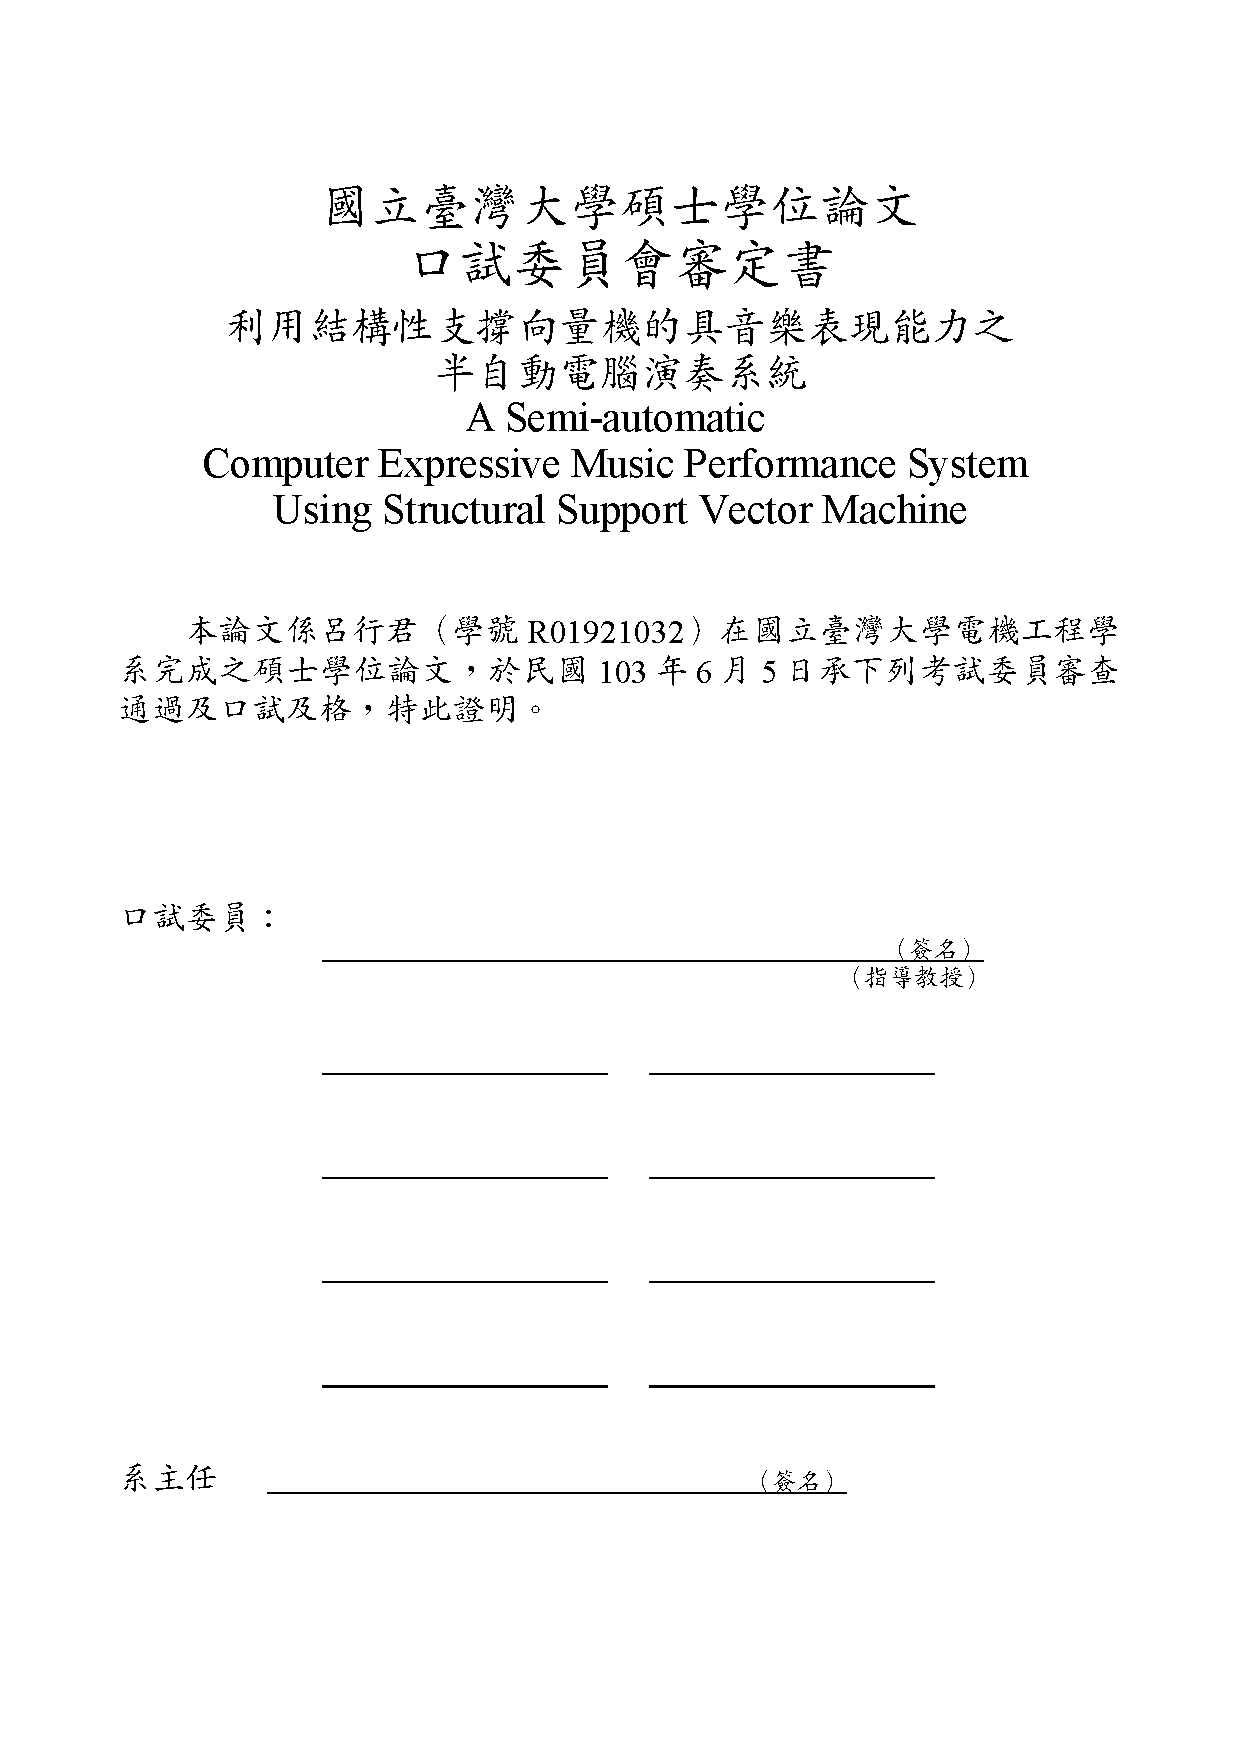
\includepdf[pages={1}]{cert.pdf}
%TODO: NTUEE Certification Document

\onehalfspacing
\begin{acknowledgementsCH}

首先要感謝鄭士康教授,早在大三選修教授的專題時(感謝大學部導師張時中教授推薦),教授就給我完全的自由,讓我能夠慢慢培養出找題目、設計實驗、上台報告以及撰寫論文的能力。每週六的meeting教授也都會給予我非常實際且切中要點的建議。

感謝各位口試委員寶貴的建議,讓這份論文能夠更加完善。謝謝王真儀教授逐字逐句的幫我訂正論文並且提供非常專業的意見。感謝王育雯教授的樂理課為我的實驗打下的基礎。也感謝陳宏銘教授的多媒體訊號處理課讓我對電腦音樂有更深的認識。

感謝JCMG的各位學長姐與同學,特別是志鴻、御仁、鴻心、彥彬、韋安、鼎棋、晟文、傳佑、如江、廉喬,每次的討論都給我許多的靈感。

感謝振宇、俞仲、鍾愛、宗緯、廉喬、智展撥出你們寶貴的時間來幫我錄製實驗用的演奏範例,你們精湛的演出讓這個實驗可以有高品質的數據可以使用。

謝謝 Intel 在這兩年多來給予我經濟上的支持還有給予我學習的機會。感謝Allen Ouyang, Robinson Do, Chuanny Shiau三位主管讓我有機會參與各種富有挑戰性的計畫,也讓我可以很自由的調配上班與上學的時間。

感謝愛樂社的各位,特別是順德、芝潔、品臻、小女王、迪西、顧門口、俊麟、子恩、乃嘉、維中、子瑩、彥彤,愛樂社燃起了我對音樂的愛,與各位共度的音樂會時光也是經常是我研究的靈感來源。

另外要特別感謝台大音樂所的教授與同學,王育雯教授的樂理課的同學們在實驗中給了我許多的幫助與建議。也特別謝謝金立群教授給予我的諸多協助:WOCMAT上的批評指教、介紹口試委員、以及幫我轉貼網路問卷。

And I would like to thank all the contributors of the open source software community, especially the contributors of Python, music21, R, Rosegarden, Musescore, and Linux Mint Debian Edition. Without your great work, this thesis can't become a reality.

感謝我的家人在這20幾年來的支持與照顧,讓我可以無憂無慮的學習與成長,在我大學與研究所最忙碌的時候,家始終是我能夠最放鬆自在的地方。

最後要感謝我的女朋友,永遠笑臉迎人,為我帶來許多的歡笑,在我為研究忙的不可開交的時候也從來不會抱怨,總是默默的支持與鼓勵我。

這份研究若沒有諸位的協助是不可能完成的,在此我獻上我要獻上最誠摯的感謝,願耶和華賜恩予你與你全家。
   \flushright 呂行 謹誌 2014.6.10







\end{acknowledgementsCH}

\begin{abstractCH}

  電腦合成的音樂一向被認為是僵硬、機械化而且沒有音樂表現能力。因此能夠產生具有表現能力的電腦自動演奏系統將會對音樂產業、個人化娛樂以及表驗藝術領域有重大的影響。在這篇論文中,我們藉由隱藏式馬可夫模型結構的結構性支撐向量機(SVM-HMM)來設計一個可以產生產生具有表現能力音樂的電腦自動演奏系統。我們邀請六位研究生錄製了克萊門蒂的小奏鳴曲集 Op. 36。我們手動將這些錄音分割成樂句,並且利用程式從中抽取出音樂特徵。這些音樂特徵藉由SVM-HMM訓練成數學模型後,可以利用這個數學模型來演奏訓練過程中沒有見過的樂譜(需要手動標注分句)。此系統目前只能支援單音旋律。問卷調查的結果顯示,對於業餘或專業的音樂家來說,本系統產生的音樂尚不能達到真人的演奏水準,但是沒有音樂背景的受試者已經無法分辨本系統產生的音樂已經與真人演奏。
  
  關鍵字:電腦自動演奏、結構性支撐向量機、支撐向量機

\end{abstractCH}

\doublespacing
\begin{abstractEN}

Computer generated music is known to be robotic and inexpressive. A computer system that can generate expressive performance potentially has significant impact on music production industry, personalized entertainment or even art. In this paper, we have designed and implemented a system that can generate expressive performance using structural support vector machine with hidden Markov model output (SVM-HMM). We recorded six sets of Muzio Clementi's Sonatina Op.36 performed by six graduate students. The recordings and scores are manually split into phrases and had their musical features automatically extracted. Using the SVM-HMM algorithm, a mathematical model of expressive performance knowledge is learned from these features. The trained model can generate expressive performances for previously unseen scores (with user-assigned phrasings). The system currently supports monophonic music only. Subjective test shows that the computer generated performances still can't achieve the same level of expressiveness of human perfromers, but quantitative similarity measures show that the computer generated performances are much similar to huamn performances than inexpressive MIDIs.

Keywords: Computer Expressive Performance, Performance Rendering, Structural SVMs, Support Vector Machines.
\end{abstractEN}

\tableofcontents

\doublespacing
\listoffigures

\listoftables

\mainmatter

\doublespacing

%----------- Include/Input your thesis here -----------
%normal cite == \input

%\chapter{Get started with \LaTeX\ }
\label{c:GetStarted}
Three common font styles in this text: 
\begin{itemize}
    \item \textbf{Item1}: \textit{Italic中文123}     
    \item \textbf{Item2}: \textbf{Bold中文123}
    \item \textbf{Item3}: \textsl{slant中文123}
\end{itemize}

About the advance latex grammer see the next section \ref{s:AdvancedFeatures}.


\section{\LaTeX\ Adavanced Features}
\label{s:AdvancedFeatures}
The following features would be introduced in the coming subsections:
\begin{itemize}
    \item SubSection \ref{ss:Fig.}: \hyperref[ss:Fig.]{\textbf{Fig.}}
    \item SubSection \ref{ss:VerbUsage}: \hyperref[ss:VerbUsage]{\textbf{Verb}}
    \item SubSection \ref{ss:VerbUsage}: \hyperref[ss:VerbUsage]{\textbf{Verb}}
    \item SubSection \ref{ss:Enumeration}: \hyperref[ss:Enumeration]{\textbf{Enumeration}}
    \item SubSection \ref{ss:Table}: \hyperref[ss:Table]{\textbf{Table}}
    \item SubSection \ref{ss:CodeDisplay}: \hyperref[ss:CodeDisplay]{\textbf{Code Display}}
    \item SubSection \ref{ss:Math}: \hyperref[ss:Math]{\textbf{Math}}
    \item SubSection \ref{ss:Algorithms}: \hyperref[ss:Algorithms]{\textbf{Algorithms}}
\end{itemize}

%==========================================================================================
\subsection{Fig.}
\label{ss:Fig.}
\begin{figure}[htpb!]
  \centering
    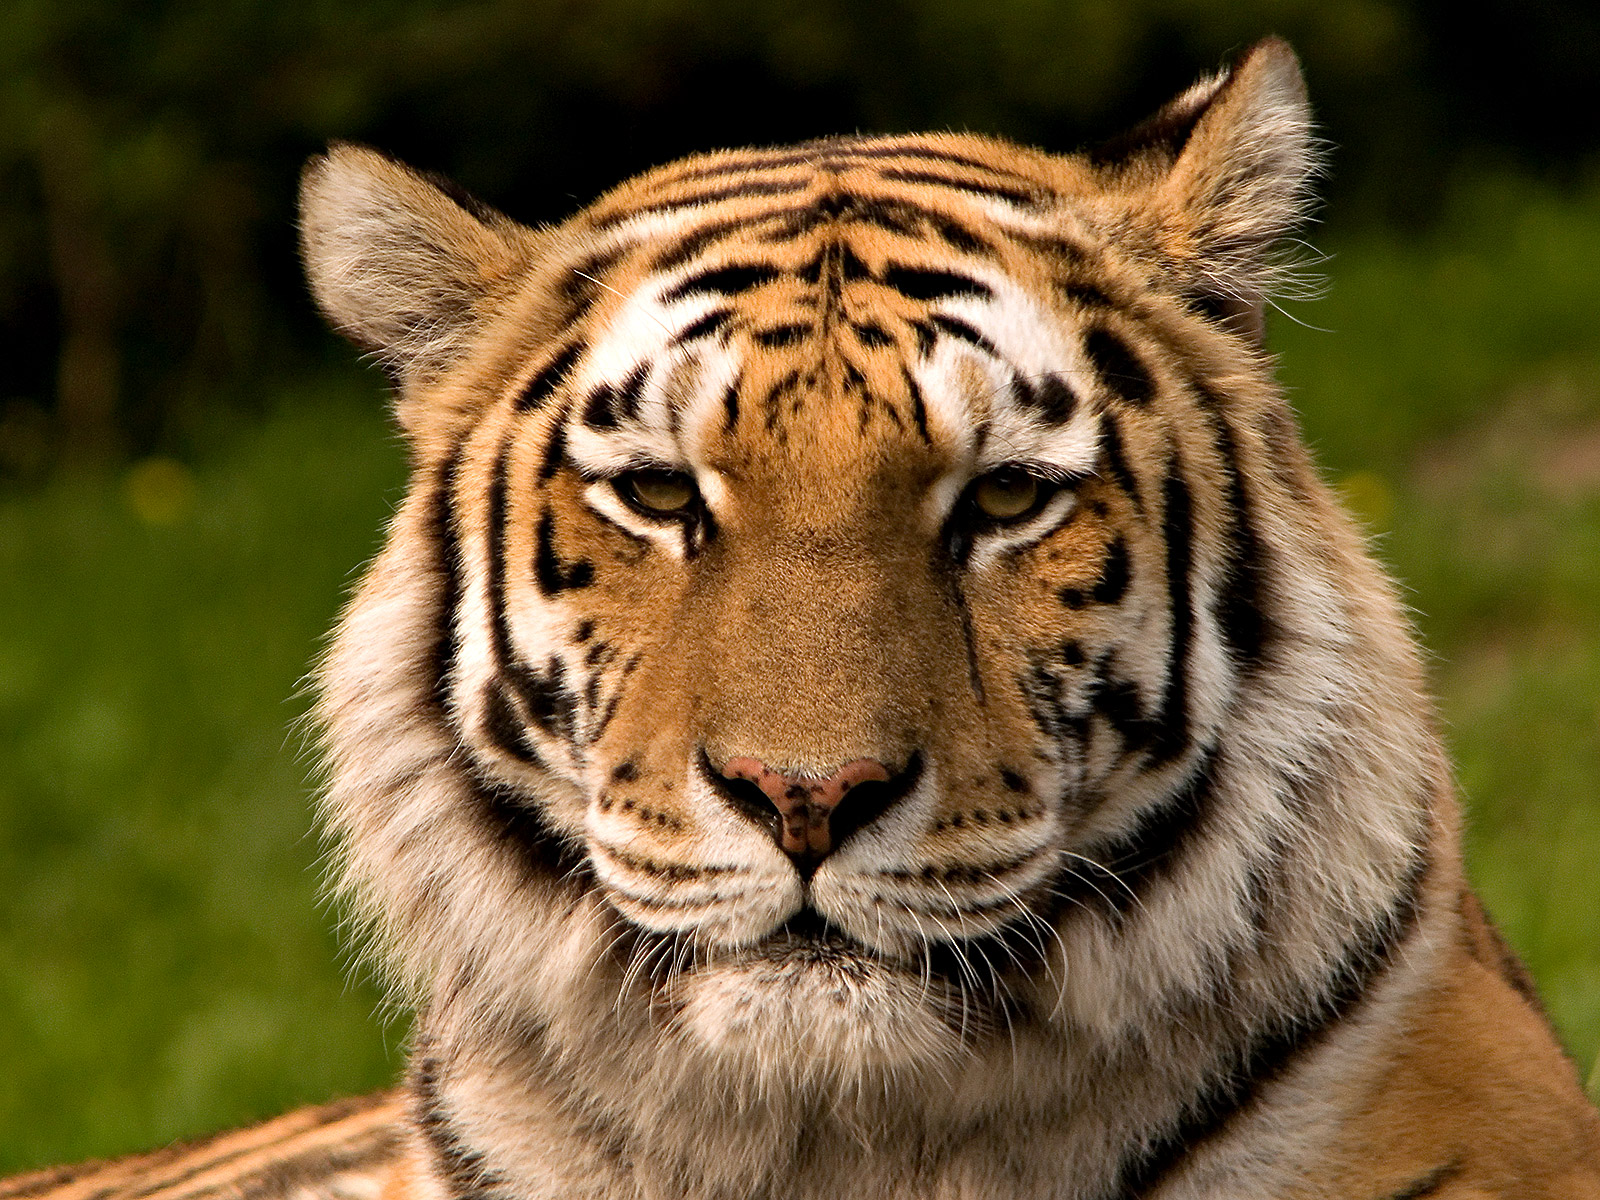
\includegraphics[width=0.5\textwidth]{fig/tiger.jpeg}
    \caption{\label{fig:tiger}A picture of a tiger.}
\end{figure}

Fig.~\ref{fig:tiger} is a picture of a tiger.


%==========================================================================================
\subsection{Table}
\label{ss:Table}

\href{http://en.wikibooks.org/wiki/LaTeX/Tables}{Table examples on WIKIBOOKS}.

\begin{table}[htpb]\begin{center}
\caption{Table Example 1}
\begin{tabularx}{8cm}{llX}
\hline
Start & End  & Character Block Name \\
\hline
3400  & 4DB5 & CJK Unified Ideographs Extension A \\
4E00  & 9FFF & CJK Unified Ideographs \\
\hline
\end{tabularx}
 \end{center}\end{table}

\begin{table}[htpb]\begin{center}
\caption{Table Example 2}
\begin{tabular}{llr}
\hline
\multicolumn{2}{c}{Item} \\
\cline{1-2}
Animal & Description & Price (\$) \\
\hline
Gnat  & per gram & 13.65 \\
      & each     &  0.01 \\
Gnu   & stuffed  & 92.50 \\
Emu   & stuffed  & 33.33 \\
Armadillo & frozen & 8.99 \\
\hline
\end{tabular}
 \end{center}\end{table}
 
 \begin{table}[htpb]\begin{center}
	\label{t:prefix-table}
	\caption{Table Example 3}
	\renewcommand{\arraystretch}{1.0}
	\begin{tabularx}{300pt}{|c|X| }
		\hline
		\multirow{1}{*}{\textbf{Allocation}} &
		Allocation, Element, Type, Script 
		\\ \hline\hline
		%------------------------------
		\multirow{6}{*}{\textbf{Data Types}} &
        Byte2, Byte3, and Byte4\\ &
        Float2, Float3, Float4\\ &
        Int2, Int3, Int4\\ &
        Long2, Long3, Long4\\ &
        Matrix2f, Matrix3f, Matrix4f\\ &
        Short2, Short3, Short4
        \\ \hline\hline
		%------------------------------
		\multirow{4}{*}{\textbf{Graphics}} &
		Mesh\\&
		ProgramFragment, ProgramRaster\\&
		ProgramStore, ProgramVertex\\&
		RSSurfaceView
		\\ \hline
		%------------------------------
	\end{tabularx}
\end{center}\end{table}

\begin{table}[htpb]\begin{center}
\caption{Table Example 4}
\begin{tabular}{|l|l|l|}
\hline
\multicolumn{3}{|c|}{Team sheet} \\
\hline
Goalkeeper & GK & Paul Robinson \\ \hline
\multirow{4}{*}{Defenders} & LB & Lucus Radebe \\
 & DC & Michael Duberry \\
 & DC & Dominic Matteo \\
 & RB & Didier Domi \\ \hline
\multirow{3}{*}{Midfielders} & MC & David Batty \\
 & MC & Eirik Bakke \\
 & MC & Jody Morris \\ \hline
Forward & FW & Jamie McMaster \\ \hline
\multirow{2}{*}{Strikers} & ST & Alan Smith \\
 & ST & Mark Viduka \\
\hline
\end{tabular}
 \end{center}\end{table}
 
 \begin{table}[htpb]\begin{center}
\caption{Table Example 5}
 \begin{tabular}{l*{6}{c}r}
Team              & P & W & D & L & F  & A & Pts \\
\hline
Manchester United & 6 & 4 & 0 & 2 & 10 & 5 & 12  \\
Celtic            & 6 & 3 & 0 & 3 &  8 & 9 &  9  \\
Benfica           & 6 & 2 & 1 & 3 &  7 & 8 &  7  \\
FC Copenhagen     & 6 & 2 & 1 & 2 &  5 & 8 &  7  \\
\end{tabular}
 \end{center}\end{table}

%==========================================================================================
\subsection{Verb}
\label{ss:VerbUsage}
Let's take a overview on how to type special characters:\\
\verb|<FRAMEWORKS_BASE>/graphics/java/android/renderscript|\\\footnote{Path of <APP\_intermediates>: <ANDROID\_ROOT>/out/target/common/obj/APPS/APPNAME\_intermediates/}
You could also go back to the beginning of the chapter by the \hyperref[c:GetStarted]{\textbf{hyperref}}.

%==========================================================================================
\subsection{Enumeration}
\label{ss:Enumeration}
\begin{enumerate}
\item Enumerated Item1
\item Enumerated Item2
\item Enumerated Item3
\end{enumerate}

%==========================================================================================
\subsection{Code Display}
\label{ss:CodeDisplay}

\lstset{
	language=C++,
	stringstyle=\rmfamily,
	commentstyle=\itshape\color[rgb]{0.133,0.545,0.133},
	showstringspaces=false,
	basicstyle=\ttfamily\scriptsize,
	numberstyle=\tiny,
	numbers=left,
	stepnumber=1,
	numbersep=10pt,
	tabsize=2,
	breaklines=true,
	prebreak = \raisebox{0ex}[0ex][0ex]{\ensuremath{\hookleftarrow}},
	breakatwhitespace=false,
  	columns=fixed,
  	upquote=true,
  	extendedchars=true,
	xleftmargin=2em,
	xrightmargin=.5em,
	escapeinside={(*@}{@*)},
    mathescape=false,
}
Here is a "Hello, DanDing." example:
\begin{lstlisting}[style=nonumbers] 
void main(int argc, char **argv)
{
    printf("   ˊ_> ˋ  ");
}
\end{lstlisting}


Another example with line numbers:
\begin{lstlisting}
void main(int argc, char **argv)
{
    printf("   ˊ_> ˋ  ");
}
\end{lstlisting}

Matlab example:

\definecolor{dkgreen}{rgb}{0,0.6,0}
\definecolor{gray}{rgb}{0.5,0.5,0.5}
\lstset{language=Matlab,
   keywords={break,case,catch,continue,else,elseif,end,for,function,
      global,if,otherwise,persistent,return,switch,try,while},
   basicstyle=\ttfamily,
   keywordstyle=\color{blue},
   commentstyle=\color{red},
   stringstyle=\color{dkgreen},
   numbers=left,
   numberstyle=\tiny\color{gray},
   stepnumber=1,
   numbersep=10pt,
   backgroundcolor=\color{white},
   tabsize=4,
   showspaces=false,
   showstringspaces=false}

\begin{lstlisting}
function y = demo(x) % This is a comment.
   str = 'hello there';
   y = x + 1;
end
\end{lstlisting}

%==========================================================================================
\subsection{Math}
\label{ss:Math}
\begin{itemize}
    \item Inline mode:\\
The solution to $\sqrt{x} = 5$ is $x=25$.
    \item Display mode:\\
The solution to \[\sqrt{x} = 5\] is \[x=25.\]
    \item Numbered mode:
\begin{equation}
2+2=4
\end{equation}
    \item Non-numbered:
\begin{equation*}
2+2=4
\end{equation*}
    \item Aligning:
\begin{align*}
2x^2 + 3(x-1)(x-2) & = 2x^2 + 3(x^2-3x+2)\\
&= 2x^2 + 3x^2 - 9x + 6\\
&= 5x^2 - 9x + 6
\end{align*}
     \item Fractions:
\[
 \frac{n!}{k!(n-k)!} = \binom{n}{k}
\]
    \item Matrix:
\[
 A_{m,n} =
 \begin{pmatrix}
  a_{1,1} & a_{1,2} & \cdots & a_{1,n} \\
  a_{2,1} & a_{2,2} & \cdots & a_{2,n} \\
  \vdots  & \vdots  & \ddots & \vdots  \\
  a_{m,1} & a_{m,2} & \cdots & a_{m,n}
 \end{pmatrix}
\]
\end{itemize}
\href{http://en.wikibooks.org/wiki/LaTeX/Mathematics}{More examples on WIKIBOOKS}.


%==========================================================================================
\subsection{Algorithms}
\label{ss:Algorithms}
%\begin{algorithm}[h]                      % enter the algorithm environment
%\caption{Calculate $y = x^n$}          % give the algorithm a caption
%\label{alg1}                           % and a label for \ref{} commands later in the document
%\begin{algorithmic}                    % enter the algorithmic environment
    %\Require $n \geq 0 \vee x \neq 0$
    %\Ensure $y = x^n$
    %\State $y \Leftarrow 1$
    %\If{$n < 0$}
        %\State $X \Leftarrow 1 / x$
        %\State $N \Leftarrow -n$
    %\Else
        %\State $X \Leftarrow x$
        %\State $N \Leftarrow n$
    %\EndIf
    %\While{$N \neq 0$}
        %\If{$N$ is even}
            %\State $X \Leftarrow X \times X$
            %\State $N \Leftarrow N / 2$
        %\Else[$N$ is odd]
            %\State $y \Leftarrow y \times X$
            %\State $N \Leftarrow N - 1$
        %\EndIf
    %\EndWhile
%\end{algorithmic}
%\end{algorithm}
\href{http://en.wikibooks.org/wiki/LaTeX/Algorithms_and_Pseudocode}{More examples on WIKIBOOKS}.



\chapter{Introduction}
\framebox{REVIEW1}
\section{Motivation}
%Robot => speech => MIDI (history)
From the machnical music performing antomata, to the Japanese virtual signer Hatune Miku, there had been many attempts to create autoated system that performs music. However, many of these system can only perform predefined expression, which is not very satisfying. State-of-the-art text-to-speech system can already generate fluid and natural speech, but computer performance still can't perform very expressivly.

Therefore, many researcher have devoted many effort to develop systems that can automatically or semi-automatically perform music expressively. There is even a biannual contest called Music Performance Rendering Contest (RenCon)\cite{RenCon} that puts all performance system to into competition. Their roadmap suggest that they wish to win the Chopin International Piano Contest by a computer perforer. We will review previous works, including many which won the RenCon prizes, in Chapter \ref{chap:prev}.
%Computer generated music, such as synthsized MIDI, are often considered robotic and unexpressive. But we have already witnessed the fluid and lively sound generated by state-of-the-art text-to-speech systems. This inspired us to develop a system that can read a music score and play it in an expressive, humanly way. Such system can be used for audiolizing score notation editing software, creating interactive media content, and generating royality-free music. 

%Established pianists always has his/her own distinctive style. Such sytle distinguised himself/herself from all the other pianists. If the expressive performance system can learn the style of a performer, it might be able to provide musicological insight of performance styles. Furthermore, we can even make a mastero who is no longer with us play music he/she never played in his/her lifetime.

There are many applications for a computer expressive performance system, many commercial music typesetting software like Finale and Sibelius already have expressive playback features built-in. On the commercial side, such system can provide personalized music listening experience. For the music production industry, it saved a lot of cost on hiring musicians or licensing. Such system can also opens up new opportunity in music making, such as human-machine co-performance, or interactive multimedia installation. In academia, researchers can use this technology to model the performing style of musicians, or restore historical music archive.

\framebox{TODO:Discuss Mazolla's theroy of expressive performance}

%\begin{figure}[tp]
%   \begin{center}
%      %TODO:Fig.: expressive performance concept
%      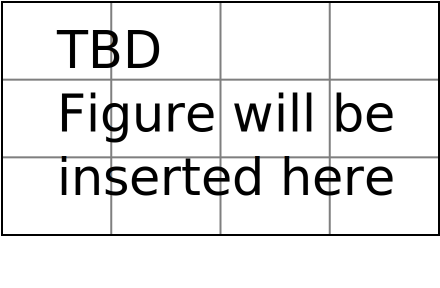
\includegraphics[width=\textwidth]{fig/TBDFigure}
%
%   \end{center}
%   \caption{From Composer to Performance}
%   \label{fig:concept}
%\end{figure}
%Application: musicology study, typesetting tool, play score archive, play computer-generated music, accompaniment



\section{Goal and Contribution}
\framebox{TODO:brief guide to previous works}
There are many different goals for computer expressive performance, which will be discussed in Chapter \ref{chap:prev}. In this research the ultimate goal is to be able to play any music in any expressive style specified. But due to the technical and time constrain, we need to set a more practical goal for our research. We wish to build a computer expressive performance system based on an offline supervised learning algorithm. The system will be able to learn any play monophonic musical phrases. The expressiveness will be at phrase level, structural or timbre related expression are not the primary concern. The performance style will be controlled by the learning material, which is traditional music notation, with human-annotated phrasing information. If only recordings from a single performer is given, it should learn the particular style of the performer.


The major contribution of this thesis is that we apply structural support vector machine on expressive performance problem. There exist no previous work that uses the discriminative learning power of support vector machine on computer expressive performance question. We also developed methods and tools to generate corpus for expressive performance system based on learning algorithms. 
%\bibliographystyle{unsrt}
%\bibliography{thesisbib}
\section{Chapter Organization}
In Chapter \ref{chap:prev}, we will give an overview of previous works and their varying goals, the works will be grouped by the way they learn performance knowledge, and finally we will discuss some additional specialities such as special instrument model or special user interaction pattern. In Chapter \ref{chap:proposed}, we will first give a brief introduction to the mathematical background of the learning algorithm, SVM-HMM. And then we will provide a top-down explanation to the proposed method. Then in Chapter \ref{chap:corpus}, we will explain how the corpus used for training is designed and implemented. Finally, In Chapter \ref{chap:exp}, we will show several experiment results and discussions. We have also included two appendixes, appendix \ref{chap:sw} presents some software tools used in this research, which may be helpful for other researchers in music and machine learning fields.

\chapter{Previous Works}
\label{chap:prev}
\section{Various Goals and Evaluation}
The general goal of a computer expressive performance system is to generate expressive music, as opposed to the robotic and dull expression of rendered MIDI. But the definition of "expressive" is very vague and ambiguous, so each research will need to define a more precise and measurable goal. The following are the most popular goals a computer expressive performance system wants to achieve:
\begin{enumerate}
   \item Perform music notations in a non-robotic way, regardless of the style.
   \item Reproduce a human performance or a musician's style.
   \item Accompany a human performer.
   \item Validate a musicological theory of expressive performance.
   \item Directly render computer composed music works.
\end{enumerate}

Some systems try to perform music notations in a non-robotic way in a general sense, without a certain style in mind. These systems has been employed in music typesetting softwares, like Sibelius \cite{sibelius}, to play the notation expressively. Most systems will implicitly achieve this goal.
%TODO:discuss the goals

Systems that are designed to reproduce certain human performance or style are usually designed or trained using a particular performer's recording as reference. One commercial example is the Zenph re-performance CD\cite{zenph}, which reproduced the performance style of Rachimaninov, it can perform pieces that Rachimaninov never played in his lifetime in his style. 
%
%
Accompaniment systems try to render expressive music that act as an accompaniment for a human performer. The challenge is that the system must be able to track the progress of a human performance and render the accompaniment in real-time. One commercial example is Cadenza\cite{cadenza}, using the technology created by Christopher Raphel\cite{chris}. It claims that it can help music student practice concertos with ease.
%
Another goal is to validate musicological theories. Musicologist may propose theories on expressive music performance, some of them may want to build a generative model to validate their assumptions. These systems may focus more on the specific phenomenon that the theory tries to explain instead of generating music that is pleasant to human. 
%
Finally, some systems combines computer composition with expressive performance. These systems have a great advantage because the intention of the composition can be shared with the performance module. Other systems that performs past compositions can only guess the composer's intention by analyzing the score notation. These systems usually has their own data structure to represent music, which can contain more information than traditional music notation, but the resulting performance system is not backward compatible with past compositions.


Because of the high diversity in the goals they want to achieve, the capability of these systems also differs a lot. The capability of a expressive performance system can be broadly categorized into the following three key indicators\cite{THEBOOK}:
\begin{enumerate}
   \item Expressive Expression Capability
   \item Polyphonic Capability
   \item Performance Creativity
\end{enumerate}

Expressive expression capability can range from very high level structural expression (e.g. tempo contrast between sections) to note level expression (e.g. onset, loudness, duration) or even sub-note expression (e.g. loudness envelop, timbre). Most systems can generate note-level expression, but higher or lower level expressions are much rare.

Polyphonic capability indicates if the system can perform polyphonic input. Polyphonic systems are more challenging than monophonic ones because they requires synchronization between voices. 

Performance creativity measures the ability of the system to create novel expression. The desired level of creativity varies from goal to goal. A system aiming to recreate human performance may want it to produce fixed expression based on the learning material, while a system that is combined with a composition system may want to create highly novel performance. 

%The goals discussed above imply different level of musical creativity. Huamn performance reproduction requires mimicry over creativity, on the other hand, system that plays its own composition can have a large range of creativity to explore. The methods employed also limits the ability of creativity, which will be discussed in the next section.
%Each system
\framebox{REVIEW1}
Each system will design different experiment and metrics to verify their goals. Thus, the self-reported results are can't be compared. The only public contest that evaluates expressive performance systems is called RenCon (Performance Rendering Contest)\cite{rencon}. RenCon is held biannually. Two scores (MIDI) will be given to participants one hour before the competition starts. The participants must generate the expressive MIDIs in the given time, and then the MIDIs will be played live on a Yamaha Disklavier piano. The audience and a jury cosists of professional musicians will give ratings for each performance. The performances are played in random order, so the audience and jury won't know the participant behind each performance, except semi-automatic ones. 

The RenCon is divided into fully automatic and semi-automatic categories. But the degree of human intervention in the semi-automatic category varies widely between systems. So it's not very fair to compare them.



\framebox{TODO: Discuss works that focus on timber only, e.g. Prof. Su's violin work}
%Each system
\section{Researches Classified by Methods Used}
%\begin{table}
%   \centering
%   \begin{tabular}{|c|c|}
%      TBD & TBD\\
%      TBD & TBD\\
%   \end{tabular}
%   \caption{List of Reviewed Systems}
%   \label{tab:prevworks}
%\end{table}
Despite the difference between goals of different expressive performance systems, all expressive performance systems must have some strategy to learn and apply performance knowledge. There are generally two approach: rule-based or machine learning-based.

Using rules to generate expressive music is probably the earliest approach. Director Musices \cite{17} is one of the early examples.   Pop-E \cite{28} is also a rule-based system which can generate polyphonic music, using its synchronization algorithm to synchronize voices. Computational Music Emotion Rule System \cite{31} tried to develop rules that express human emotions.  Other systems like Hierarchical Parabola System \cite{17}\cite{18}\cite{19}\cite{20}, Composer Pulse System\cite{21,22}, Bach Fugue System\cite{23}, Trumpet Synthesis System \cite{24, 25} and Rubato \cite{26, 27} are also some systems that use rules to generate expressive performance. Most of the systems focus on expressive attributes like note onset, note duration and loudness, but Hermode Tuning System \cite{29} put special emphasis on intonation. Rule-based systems are generally more computationally efficient because the mathematical model is much simple than those learned by machine learning algorithms. And rules are generally more understandable to human than complex model parameters. But some of the nuance, such as some subconscious deviation or grouping of notes, may be hard to describe by rules, so there is a emperical limit on how complex the rule-based system can be. Lack of creativity is also a problem for rule-based approach.

Another approach is to acquire performance knowledge by machine learning. Many machine learning methods have already been applied to this problem. For example, Music Interpretation System \cite{32,33,34} and CaRo \cite{35,36,37} both use linear regression to learn performance knowledge. But it is very unlikely that the expressive performance problem is a linear system, so Music Interpretation System try to solve it by using AND operations on linear regression results to handle non-linearity. But linear regression is still an oversimplification for such problem.

More complicated algorithms have also been applied: ANN Piano \cite{38} and Emotional flute \cite{39} uses artificial neural network. ESP Piano \cite{55} and Music Plus One \cite{52,53,54} uses Statistical Graphical Models such as Hidden Markov Model (HMM) and Bayesian Belief Network, but they did no use structural support vector machine to train the HMM.%, although the later one focus more on accompaniment task rather than rendering notation. 
KCCA Piano System \cite{57} uses kernel regression. Drumming System \cite{82} tried different mapping models that generates drum patterns.

Evolutionary computation such as genetic programming is used in Genetic Programming Jazz Sax \cite{88}. Other examples include the Sequential Covering Algorithm Genetic Algorithm\cite{59}, Generative Performance Genetic Algorithm \cite{89} and Multi-Agent System with Imitation \cite{60, 93}. Evolutionary computation takes long training time, and the results are unpredictable. But unpredictable also means there are more room for performance creativity, so these system can create unconventional but interesting performances.

\framebox{TODO: Discuss works that focus on timber only, e.g. Prof. Su's violin work}
Another approach is to use case-based reasoning. SaxEx\cite{40,41,42} use fuzzy rules based on emotions to generate Jazz saxophone performance. Kagurame \cite{43,44} focus on style (Baroque, Romantic, Classic etc.) instead of emotion. Ha-Hi-Hun \cite{45} has a more ambitions goal in mind: to accept natural language instructions like \enquote{Perform piece X in the style of Y.} Another series of researches done by Widmer at el., called PLCG \cite{46, 47, 48} uses data-mining to find rules for expressive performance. It's successor Phrase-decomposition/PLCG \cite{49} added hierarchical phrase structures support to the original PLCG system. And the latest research in the series called DISTALL \cite{50, 51} added hierarchical rules to the original one.

Most of the of the performance systems discussed above takes digitalized traditional musical notation (MusicXML etc.) or neutral audio as input. They have to figures out the expressive intention of the composer by musical analysis or assigned by the user. But another type of computer expressive performance has a great advantage over the previous ones, by combining computer composition and expressive performance, the performance module can share the performance intention directly with the composition module. Ossia \cite{61} and pMIMACS \cite{pmimacs} are two examples of this category.  This approach provides great possibility for creativity, but they can only play their own composition, which is rather limited.

%\framebox{TODO:Fig.:selected figures from previous works}
\section{Additional Specialties}

Most expressive performance systems implicitly or explicitly generates piano performance, because it's relatively easy to collect training samples for piano and piano sound is relatively easy to synthesize. Yet, some systems generates music in other instruments, such as saxophone\cite{40, 41, 42}, trumpet\cite{24, 25}, flute \cite{39} and drums \cite{56}. These systems requires extra effort in creating instrument models in training, generation and synthesizing. 

If not specified, most systems handles traditional western tonal music. However, most saxophone-based works\cite{40, 41, 42} generates Jazz music, because saxophone is an iconic instrument in Jazz performance. And the Drumming System\cite{56} generates Brazilian drumming music.%The Bach Fugue System \cite{23}, literally, focus on fugue works composed by bach. 

Performing polyphonic music is much more challenging than monophonic music, because it requires synchronization between voices, while allowing each voice to have their own expression at the same time. Pop-E\cite{28} use a synchronization mechanism to achieve polyphonic performance. Bach Fugue System \cite{23} is created using the polyphonic rules in music theory about fugue, so it's inherently able to play polyphonic fugue. KCCA Piano System \cite{57}can generate homophonic music -- an upper melody with an accompaniment -- which is common in piano music.   Music Plus One \cite{52,53,54} is a little bit different because it's a accompaniment system, it adapts non-expressive orchestral accompaniment track to user's performance. Other systems usually generates monophonic tracks only. 

\framebox{REVIEW1}

%%\chapter{Theoretical Background}
%\framebox{REVIEW1}
\section{A Brief Introduction to SVM-HMM}
\label{sec:svm-hmm}
In this thesis, we use structural support vector machine to learn performance knowledge from expressive performance samples. Unlike traditional SVM algorithm, which can only produce univariate prediction, structural SVM can produce structural predictions like tree, graph or sequence. Structural SVM with hidden Markov model output (SVM-HMM) has been successfully applied to part-of-speech tagging problem\cite{svm2009}. The part-of-speech tagging problem has some similarity with expressive performance problem. In part-of-speech tagging, one tries to identify the role by which the word plays in the sentence, while in expressive performance, one tries to determine how a note should be played, usually based on it's role in the musical phrase. %For example, an authentic cadence at the end of a phrase is usually played louder and stronger than a embellishment note in the middle of a phrase. 
Thus, we believe SVM-HMM will be a good candidate for expressive performance. The following introduction and formulas relies heavily on \cite{svm2009, svm2005, svm2003}.

%Ref: 20130420 slides

%TODO:discuss traditional SVM here?
Traditional SVM prediction problem can be described as finding a function 
$$h: \mathcal{X \rightarrow Y}$$ with lowest prediction error. $\mathcal{X}$ is the input features space, and $\mathcal{Y}$ is the prediction space. In traditional SVM, elements in $\mathcal{Y}$ are labels (classification) or real values (regression). But structural SVM extends the framework to generate structural output, such as tree, graph or sequence.
To extend SVM to support structured output, the problem is modified as finding a discriminant function $$F: \mathcal{X} \times \mathcal{Y} \rightarrow \mathcal{R}$$, in which the input/output pairs are mapped to a real number score. To predict an output $y$ for an input $x$, one try to maximize $F$ over all $y \in \mathcal{Y}$. 

$$f(x) = \argmax_{y\in\mathcal{Y}} F(w,x,y)$$

Let $F$ be a linear function of the form:

$$ F = \mathbf{w}^{T}\Psi(x,y)$$, 
where $\mathbf{w}$ is the parameter vector, and $\Psi(x,y)$ is the kernel function relating input $x$ to output $y$. $\Psi$ can be defined to accommodate various kind of structures. 

%emprical risk
For each structure we want to predict, a loss function that measures the accuracy of of a prediction is required. A loss function $\Delta:\mathcal{Y}\times\mathcal{Y}\rightarrow R$ need to satisfy the following property:

$$\Delta(y, y') \geq 0 \ for\ y \neq y'$$
$$\Delta(y, y) = 0 $$

The loss function is assumed to be bounded. Let's assume the input-output pair $(x,y)$ is drawn from a join distribution P(x,y), the prediction problem is to minimize the total loss:

%TODO: total loss formula 2005 sec 2.1
$$R_p^\Delta = \int_{\mathcal{X} \times \mathcal{Y}} \Delta (y, f(x))dP(x,y)$$

Since we can't directly find the distribution $P$, we need to replace this total loss with a empirical loss, which can be calculated from the observed training set of $(x_i, y_i)$ pairs.
%TODO: emprical loss
$$R_s^\Delta(f) = \frac{1}{n}\sum^n_{i=1}\Delta(y_i, f(x_i))$$

Now we are ready to extend SVM to structural output, starting with a linear separable case, and we will then extend it to soft-margin formulation. 

A linear separable case can be expressed by a set of linear constrains
%TODO: 2005 formula 4
$$\forall i \in \{1,\cdots,n\}, \forall \hat{y_i}\in\mathcal{Y}: \mathbf{w}^T [\Psi(x_i, y_i) - \Psi(x_i, \hat{y_i})]\geq 0$$

The constrains imply that the groundtruth $y_i$ for $x_i$ has the minimum $F$ value than any other $\hat{y}_i \neq {y_i}$.

The key concept of SVM is the large margin principle. We not only want to find a solution that statisfies the constrains, but also we want to maximize the margin between the groundtruth and the second best $\hat{y}_i$:
%TODO: 2005 formula 4+
$$
\begin{aligned}
& \max_{\gamma, \mathbf{w}:\|\mathbf{w}\| = 1} \gamma \\
& s.t \; \forall i \in \{1,\cdots,n\}, \forall \hat{y_i} \in\mathcal{Y}: \mathbf{w}^T [\Psi(x_i, y_i) - \Psi(x_i, \hat{y_i})] \geq \gamma\\
\end{aligned}
$$

, which is equivalent to the convex quadratic programming problem:
%TODO: 2005 formula 5,k 6
$$
\begin{aligned}
   & \min_{\mathbf{w}, \xi_i \geq 0} \frac{1}{2}\|\mathbf{w}\|^2 \\\
    &s.t.\; \forall i \in \{1,\cdots,n\},\hat{y_i} \in \mathcal{Y}: \mathbf{w}^T[\Psi(x_i,y_i) - \Psi(x_i,\hat{y_i})] \geq 1\\
\end{aligned}
$$

To extend the linear-separable case to non-separable case, slack variables $\xi_i$ can be introduced to penalize prediction errors, results in a soft-margin formalization:
%TODO: 2005 formula SVM1
$$
\begin{aligned}
   & \min_{\mathbf{w}, \xi_i \geq 0} \frac{1}{2}\|\mathbf{w}\|^2 + \frac{C}{n}\sum^n_{i=1}\xi_i\\
    &s.t.\; \forall i \in \{1,\cdots,n\},\hat{y_i} \in \mathcal{Y}: \mathbf{w}^T[\Psi(x_i,y_i) - \Psi(x_i,\hat{y_i})] \geq 1 - \xi_i \\
\end{aligned}
$$

$C$ is the weighting parameter controlling the trade-off between low training error and large margin. The optimal $C$ varies between different problems, so experiment should be conducted to find the optimal $C$ for our problem.

Intuitively, a constrain violation with larger loss should be penalize more than the one with smaller loss. So I. Tsochantaridis et al. \cite{svm2005} proposed two possible way to take the loss function into account. The first way is to re-scale the slack variable by the inverse of the loss, so a high loss leads to smaller re-scaled slack variable:
%slack rescaling

$$
\begin{aligned}
   & \min_{\mathbf{w}, \xi_i \geq 0} \frac{1}{2}\|\mathbf{w}\|^2 + \frac{C}{n} \sum^n_{i=1}\xi_i\\
    &s.t.\; \forall i \in \{1,\cdots,n\},\hat{y_i} \in \mathcal{Y}: \mathbf{w}^T[\Psi(x_i,y_i) - \Psi(x_i,\hat{y_i})] \geq 1 - \frac{\xi_i}{\Delta(y_i, \hat{y_i})} \\
\end{aligned}
$$

The second way is to re-scale the margin, which yields 
%margin-rescaling
$$
\begin{aligned}
   & \min_{\mathbf{w}, \xi_i \geq 0} \frac{1}{2}\|\mathbf{w}\|^2  + \frac{C}{n} \sum^n_{i=1}\xi_i\\
    &s.t.\; \forall i \in \{1,\cdots,n\},\hat{y_i} \in \mathcal{Y}: \mathbf{w}^T[\Psi(x_i,y_i) - \Psi(x_i,\hat{y_i})] \geq \Delta(y_i, \hat{y_i}) - \xi_i\\
%
\end{aligned}
$$
In the implementaion we use, we use margin re-scaling.

But the above quadratic programming problem has a very large number ($O(n|\mathcal{Y}|)$) of constrains, which will take considerable time to solve. I. Tsochantaridis et al. \cite{svm2005} proposed a greedy algorithm to speed up the process by selecting only part of the constrains that contributes the most to finding the solution. Initially, the solver starts with an empty working set containing no constrains. Than the solver iteratively scans the training set to find the most violated constrains under the current solution. If a constrain is violated more times than a desired threshold, the constrain is added to the working set of constrains. Then the solver re-calculate the solution under the new working set. The algorithm will terminate once no more constrain can be added under the desired precision.

In a later work by Joachims et al.\cite{svm2009}, they created a new formulation and algorithm to further speed up the algorithm. Instead of using one slack variables for each training sample, which results in a total of $n$ slack variables, they use a single slack variable for all $n$ training samples. The following formula is the 1-slack version of slack-rescaling structural SVM:
%1-slack
$$
\begin{aligned}
    & \min_{\mathbf{w}, \xi_i \geq 0} \frac{1}{2}\|\mathbf{w}\|^2  + C \xi\\
    &s.t.\; \forall i \in \{1,\cdots,n\},\hat{y_i} \in \mathcal{Y}: \mathbf{w}^T[\Psi(x_i,y_i) - \Psi(x_i,\hat{y_i})] \geq \frac{1}{n}\sum^n_{i=1}1 - \frac{\xi}{\Delta(y_i, \hat{y_i})} \\
\end{aligned}
$$

And margin-rescaling structural SVM:

$$
\begin{aligned}
    & \min_{\mathbf{w}, \xi_i \geq 0} \frac{1}{2}\|\mathbf{w}\|^2  + C \xi\\
    & s.t.\; \forall i \in \{1,\cdots,n\},\hat{y_i} \in \mathcal{Y}: \mathbf{w}^T[\Psi(x_i,y_i) - \Psi(x_i,\hat{y_i})] \geq \frac{1}{n}\sum^n_{i=1}\Delta(y_i, \hat{y_i}) - \xi \\
\end{aligned}
$$
%                $$\min_{\mathbf{w}, \xi_i \geq 0} \frac{1}{2}\mathbf{w}^T\mathbf{w} + \frac{C}{n} \sum_{i=1}^{n} \xi_i$$
%                s.t. for $i = 1\cdots n$
%                $$\forall \hat{y_i} \in \mathcal{Y}: \mathbf{w}^T[\Psi(x_i,y_i) - \Psi(x_i,\hat{y_i})] \geq \Delta(y_i, \hat{y_i}) - \xi_i $$
%
%                $$\forall \hat{y_i} \in \mathcal{Y}: \mathbf{w}^T[\Psi(x_i,y_i) - \Psi(x_i,\hat{y_i})] \geq 1 - \frac{\xi+i}{\Delta(y_i, \hat{y_i})}$$
Detailed proof on how the new formulation is equally general as the old one is given in the paper \cite{svm2009}.

With the framework described above, the only problem left is how to define the general loss function and $\Psi$ for our problem? Drawing the inter-state dependencies and time dependencies concept from hidden Markov model, Y. Altun et al.\cite{svm2003} proposed two types of features for a equal-length observation/label sequence pair $(x,y)$. The first is the interaction of a observed feature $x^s$ with a label $y^t$, the other is the interaction between neighboring labels $y^s$ and $y^t$. 

%   \begin{figure*}[tp]
%      \begin{center}
%         \includegrapsics[width=0.8\textwidth]{fig/TBDFigure}
%      \end{center}
%      \caption{Hidden Markov Model}
%      \label{fig:hmm}
%   \end{figure*}

To illustrate the method, we use a example from music: for some observed features $\Psi_r(x^s)$ of a note $x$ located in $s$-th position of the phrase, and assume $\left[ \left[ y^t = \tau \right] \right]$ denotes the $t$-th note is played at a velocity of $\tau$, the interaction of the observed feature and the label can be written as:
%TODO hmm 3 formula 4
$$\psi^{st}_{r\sigma}(\mathbf{x}, \mathbf{y}) = \left[\left[y^t = \tau \right] \right]\Psi_r(x^s),\; 1\leq\gamma\leq d,\; \tau \in \Sigma $$

And the interaction between labels can be written as:
%TODO hmm 3 formula 5
$$\hat{\psi}^{st}_{r\sigma}(\mathbf{x}, \mathbf{y}) = \left[\left[y^s = \sigma \wedge y^t = \tau \right] \right],\; \sigma, \tau \in \Sigma $$

By selecting a order of dependency for the HMM model, we can further restrict $s$'s and $t$'s. For example, for a first-order HMM, $s = t$ for the first feature, and $s = t-1$ for the second feature. The two features on the same time $t$ is then stacked into a vector $\Psi(x,y;t)$. The feature map for the whole sequence is simply the sum of all the feature vectors 

%TODO hmm 3 formula 6
$$\Psi(\mathbf{x}, \mathbf{y}) = \sum^T_{t=1}\Psi(\mathbf{x}, \mathbf{y};t)$$

The distance, i.e. the general loss function, between two feature maps depends on the number of common label segments and the inner product between the input features sequence with common labels.


$$\Delta(\Psi(\mathbf{x}, \mathbf{y}), \Psi(\mathbf{\hat{x}}, \mathbf{\hat{y}})) = \sum_{s,t}\left[\left[y^{s-1} = \hat{y}^{t-1}\wedge y^s = \hat{y}^t\right] \right] + \sum_{s,t}\left[\left[y^{s} = \hat{y}^{t}\right] \right]k(x^s, \hat{x}^t)$$

Finally, during the prediction process, a Viterbi-like decoding algorithm is used to effeciently find a $y$ that maximize $F$.


%TODO: how to define loss function for HMM?
%(2003) section 3
%ovserved output <--> tag
%previous tag <--> this tag (1-order markov)
% Psi = each note's above two property summed up
%similarity = same prev tag <--> this tag sequence + same tag <--> observed output distance

%Hard-margin one
%Soft-margin one => introduce slack variable 
%Example with large loss should be emphasized => slack rescaling
%Margin can also be scaled => margin rescaling
%There are too many constrains => greedy algo (2005), select a subset of constrains from the most violated constrains to solve
%To speed up, n-slack variables are reduced to 1-slack variable (2009)

%           \item Prediction error (risk):
%               $$R^\Delta_p(h) = \int_{\mathcal{X}\times\mathcal{Y}}\Delta(y, h(x)) dP(x,y)$$
%               \begin{tabular}{ll}
%                   where & $\Delta()$ is the loss function \footnote{Must satisfy $\Delta(x,x) = 0$, $\Delta(x,y) > 0$}\\
%                   & P(x,y) is the joint distribution of $\mathcal{X}$ and $\mathcal{Y}$
%               \end{tabular}

%    \begin{frame}{Emperical Risk}
%       \begin{itemize}
%           \item Emperical Risk from training sample $S$:\footnote{Emperical Risk Minimization Priciple (Vapnik V (1998) Statistical Learning Theory. Wiley, Chichester, GB)}

%               $$R^\Delta_S(h) = \frac{1}{n}\sum_{i=1}^{n}\Delta(y_i, h(x_i))$$
%                   where  $\Delta()$ is the loss function 

%           \item Classification SVM

%                   $$\displaystyle \min_{\mathbf{w}, \xi_i \geq 0} \frac{1}{2}\mathbf{w}^T\mathbf{w} + \frac{C}{n} \sum_{i=1}^{n} \xi_i$$
%                   s.t. $$\forall i\in {1,\cdots n}: y_i (\mathbf{w}^T x_i) \geq 1-\xi_i$$
                  

%           \item Learn a discriminant function $f:\mathcal{X} \times \mathcal{Y} \rightarrow \Re$ 
%           \item Given $x$, maximizing $f$ over all $y \in \mathcal{Y}$
%               $$h_\mathbf{w} (x) = \argmax_{y\in\mathcal{Y}} f_\mathbf{w} (x,y)$$
%           \item 
%               in which $$f_\mathbf{w} (x,y) = \mathbf{w}^T{\Psi}(x,y)$$
%               \begin{tabular}{ll}
%                   where & $\mathbf{w} \in \Re^N$ is a parameter vector\\
%                         & $\Psi(x,y)$ is a feature vector relating $x$ and $y$
%               \end{tabular}
              

 
% \section{Structural SVM}

% \section{Theoretical Details}
% %&=& &=& &=& &=& &=& &=& &=& &=& =
%    \begin{frame}{Lowest Risk}
%       \begin{itemize}
%           \item Prediction error (risk):
%               $$R^\Delta_p(h) = \int_{\mathcal{X}\times\mathcal{Y}}\Delta(y, h(x)) dP(x,y)$$
%               \begin{tabular}{ll}
%                   where & $\Delta()$ is the loss function \footnote{Must satisfy $\Delta(x,x) = 0$, $\Delta(x,y) > 0$}\\
%                   & P(x,y) is the joint distribution of $\mathcal{X}$ and $\mathcal{Y}$
%               \end{tabular}

%           %\item Training sample: $(x_1, y_1), (x_2, y_2), \cdots$ where $y_i$'s may have structural relationship
              
%       \end{itemize}
%    \end{frame}
%    \begin{frame}{Emperical Risk}
%       \begin{itemize}
%           \item Emperical Risk from training sample $S$:\footnote{Emperical Risk Minimization Priciple (Vapnik V (1998) Statistical Learning Theory. Wiley, Chichester, GB)}

%               $$R^\Delta_S(h) = \frac{1}{n}\sum_{i=1}^{n}\Delta(y_i, h(x_i))$$
%                   where  $\Delta()$ is the loss function 

%           %\item Training sample: $(x_1, y_1), (x_2, y_2), \cdots$ where $y_i$'s may have structural relationship
              
%       \end{itemize}
%    \end{frame}

%    \begin{frame}{Traditional SVM}
%       \begin{itemize}
%           \item Classification SVM

%                   $$\displaystyle \min_{\mathbf{w}, \xi_i \geq 0} \frac{1}{2}\mathbf{w}^T\mathbf{w} + \frac{C}{n} \sum_{i=1}^{n} \xi_i$$
%                   s.t. $$\forall i\in {1,\cdots n}: y_i (\mathbf{w}^T x_i) \geq 1-\xi_i$$
                  

              
%       \end{itemize}
%    \end{frame}

%    \begin{frame}{Structural SVM}
%       \begin{itemize}
%           \item Extend SVM for structural output
%           \item Learn a discriminant function $f:\mathcal{X} \times \mathcal{Y} \rightarrow \Re$ 
%           \item Given $x$, maximizing $f$ over all $y \in \mathcal{Y}$
%               $$h_\mathbf{w} (x) = \argmax_{y\in\mathcal{Y}} f_\mathbf{w} (x,y)$$
%           \item 
%               in which $$f_\mathbf{w} (x,y) = \mathbf{w}^T{\Psi}(x,y)$$
%               \begin{tabular}{ll}
%                   where & $\mathbf{w} \in \Re^N$ is a parameter vector\\
%                         & $\Psi(x,y)$ is a feature vector relating $x$ and $y$
%               \end{tabular}


                  

              
%       \end{itemize}
%    \end{frame}

%    \begin{frame}{N-slack Formulations}
%       \begin{itemize}
%           \item margin-rescaling: change hinge, fixing slope
%              $$\Delta_{MR}(y,h_\mathbf{w}) = \max_{\hat{y} \in \mathcal{Y}} \{ \Delta(y, \hat{y}) - \mathbf(x)^T {\Psi}(x,y) + \mathbf{w}^T{\Psi}(x,\hat{y}\} \geq \Delta(y,h_\mathbf{w}(x))$$
%           \item slack-rescaling: fixing hinge, changing slope
%              $$\Delta_{SR}(y,h_\mathbf{w}) = \max_{\hat{y} \in \mathcal{Y}} \{ \Delta(y, \hat{y}) (1 - \mathbf(x)^T {\Psi}(x,y) + \mathbf{w}^T{\Psi}(x,\hat{y} )\} \geq \Delta(y,h_\mathbf{w}(x))$$
              
%       \end{itemize}
%    \end{frame}

%    \begin{frame}{Optimization Problems}
%       \begin{itemize}
%           \item
%                $$\displaystyle \min_{\mathbf{w}, \xi_i \geq 0} \frac{1}{2}\mathbf{w}^T\mathbf{w} + \frac{C}{n} \sum_{i=1}^{n} \xi_i$$
%                s.t. for $i = 1\cdots n$
%           \item n-slack structural SVM w/ margin-rescaling
%                $$\forall \hat{y_i} \in \mathcal{Y}: \mathbf{w}^T[\Psi(x_i,y_i) - \Psi(x_i,\hat{y_i})] \geq \Delta(y_i, \hat{y_i}) - \xi_i $$

%           \item n-slack structural SVM w/ slack-rescaling
%                $$\forall \hat{y_i} \in \mathcal{Y}: \mathbf{w}^T[\Psi(x_i,y_i) - \Psi(x_i,\hat{y_i})] \geq 1 - \frac{\xi+i}{\Delta(y_i, \hat{y_i})}$$
%       \end{itemize}
%    \end{frame}

%    \begin{frame}{1-Slack Formulation}
%       \begin{itemize}
%           \item
%       \end{itemize}
%    \end{frame}


%TODO: theoratical background


%\section{Brent's Method}
%\section{diff}
 %theoratical background is merged to propsed method, becasuse it has only one section
\chapter{Proposed Method}
%TODO: START COPY-PASTE
\section{Overview}
   %input output only melodic constrins
   %flow chart
      \begin{figure*}[tp]
         \begin{center}
            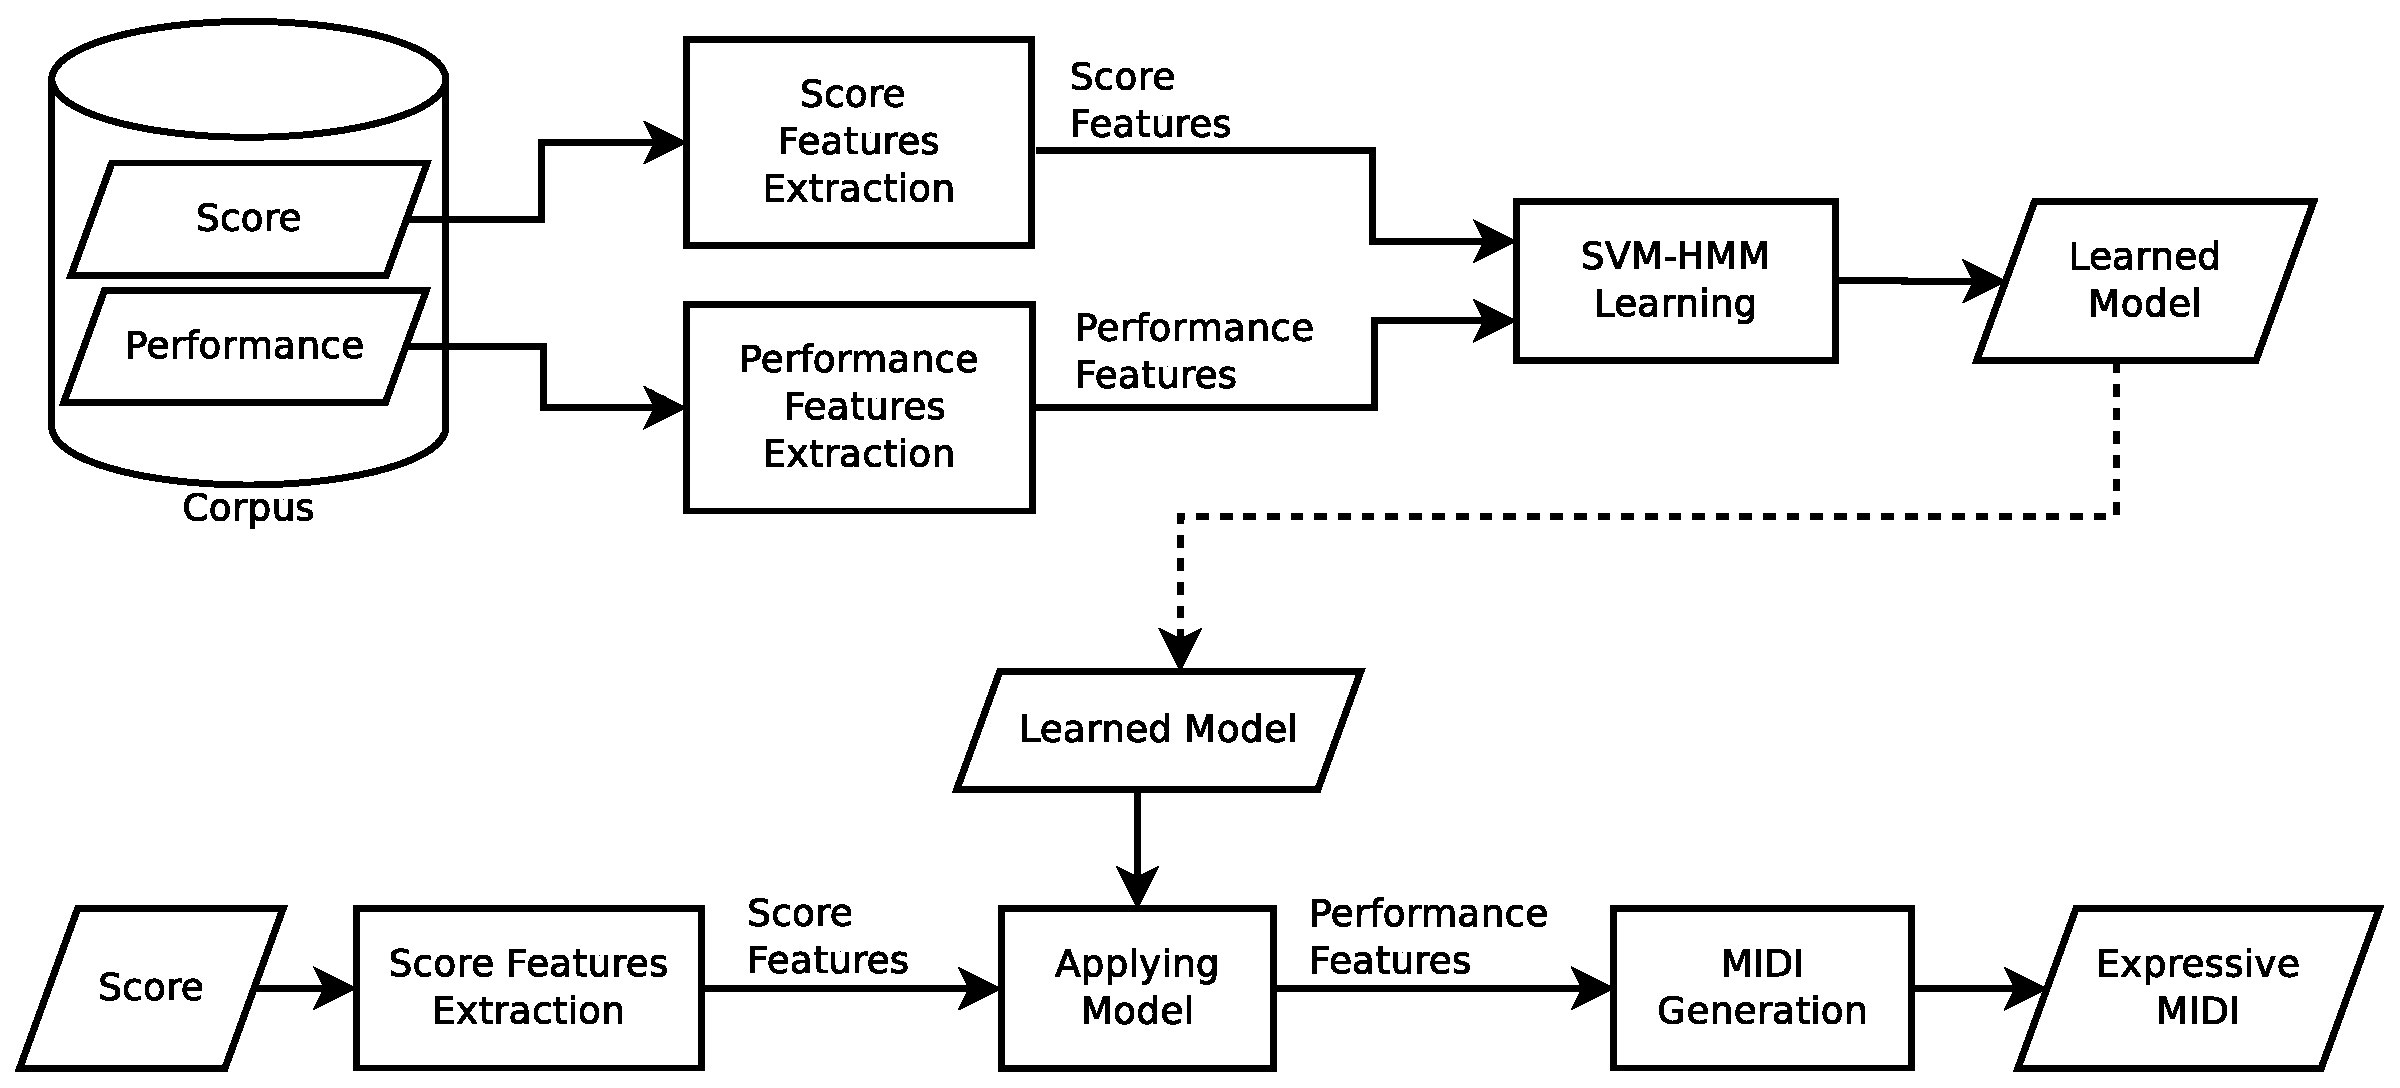
\includegraphics[width=\textwidth]{fig/sys_arch}
         \end{center}
         \caption{System Architecture} 
         \label{fig:flow}
      \end{figure*}
The high-level archtecture of the purposed system is shown in figure \ref{fig:flow}. The system is has two phases, the upper half of the figure is the learning phase, while the lower half is the generating phase.  In the training phase, score and expressive performance recording pairs are feed in, their features will be extracted and used as the input for the learning algorithm.  The learning algorithm will produce a learned model, which can be used to generate expressive performance hereafter. In the generating phase, a score is taken as input, and it's score features are extracted. The generation module ("Applying Model" box) then use the extracted features and the learned model to produce the preformance features for the score. The performance features can be viewed as the instruction for expression. With these features, an expressive MIDI performance for the input score can easily be generated.  
%TODO: refer to feature exction and corpus chapter

The system is not intend to add fixed expression to all pieces. Rather it is intended to perform music according to the style which the user wants. This kind of user interactivity can be achieved in two ways: first, the user can choose the training dataset. The dataset is organized by tags, example of tags are like performer, mood, emotion, genre, style, etc. So the user can select a subset of training sample by selecting tags. Second, the phrasing is given by the user. Since phrasing controls the overall structural interpretation of a music piece, and form a breathing feeling in music, user is given direct control over the performance.

There are still some constrains for the system now. The scores must be monophonic and contains only one musical phrase. One has to manully label the phrasing for any scores used. The learning algorith, namely structural suppor vector machine, can only perform offline learning, so the learning phase can only work in a non-realtime scenario. The generating phase can work much faster though, it can procude expressive music almost instantely after loading the score. All the scores are loaded in batch, the systme currently don't accept streaming input.

   \section{Features}
   The system is trying to mimic the process of human performance: the musican reads the explict and implict cues from the score and transform them into musical expressions. So the features can be categorized into two category: score features and performance features.  Score features are information contained in the score. Performance features corresponds to the musical expression. The basic time unit for both features are a note. 
      \subsection{Score Features}
      Score features includes:
      \begin{description}
         \item [Relative position in a phrase:]
            The relative position of a note in the phrase. From 0\% to 100\%. This feature can catch the musical hint of the opening and closing of a phrase.  
         \item [Relative pitch:]
            The pitch (in semitone) of a note relative to the pitch range of the phrase. For a phrase of $n$ notes with pitch $P_1, P_2, \dots, P_n$, $$RP = \frac{P_i -min(P_1, P_2, \dots, P_n) }{max(P_1, P_2, \dots, P_n)-min(P_1, P_2, \dots, P_n) }$$  Where $P_i$ is the pitch of note at position $t$

         \item [Interval from the previous note:] The direction of melody movement. Measured in semitone. $$IP = P_{i} - P_{i-1} $$ See figure \ref{fig:interval} for example.
         \item [Interval to the next note:] The direction of melody movement. $$IN = P_{i+1} - P_i$$ See figure \ref{fig:interval} for example.
         
      \begin{figure}[tp]
         \begin{center}
            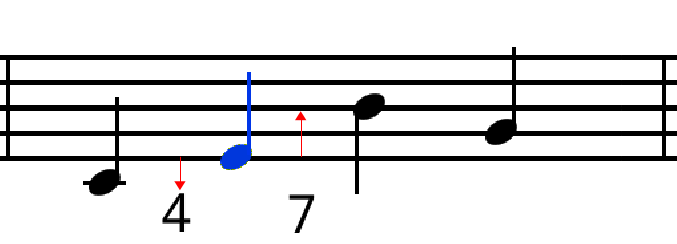
\includegraphics[width=0.4\textwidth]{fig/interval_arrow}
         \end{center}
         \caption{Interval from/to neighbor notes}
         \label{fig:interval}
      \end{figure}

         
         \item [Note duration:] The duration of a note in beats.
         \item [Relative Duration with the previous note:] The duration of a note divided by the duration of its previous note. For a phrase of $n$ notes with duration $D_1, D_2, \dots, D_n$, $$RDP = \frac{D_i}{D_{i-1}} $$ See figure \ref{fig:duration} for example.
         \item [Relative duration with the next note:] The duration of a note divided by duration of its next note. $$RDN = \frac{D_i}{D_{i+1}} $$ See figure \ref{fig:duration} for example.

      \begin{figure}[tp]
         \begin{center}
            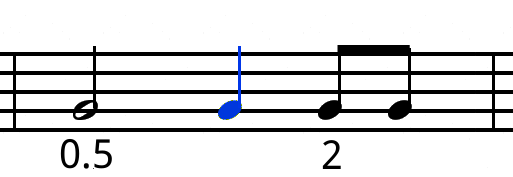
\includegraphics[width=0.4\textwidth]{fig/duration}
         \end{center}
         \caption{Duration from/to neighbor notes}
         \label{fig:duration}
      \end{figure}
   \item [Metric position:] The position of a note in a measure, measured by the beat unit defined by the time signature. For example, a $^4_4$ time signature will have a beat unit of a quarter note. So if the measure consists of four quarter notes, each of them will have metric position of 1, 2, 3 and 4. See figure \ref{fig:metrical}.

   \begin{figure}[tp]
      \begin{center}
         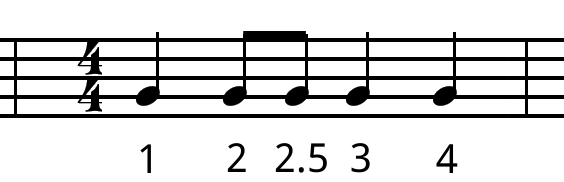
\includegraphics[width=0.4\textwidth]{fig/metrical}
      \end{center}
      \caption{Metric position}
      \label{fig:metrical}
   \end{figure}
      \end{description}

      \subsection{Performance Features}
      Performance features includes:
      \begin{description}
         \item [Relative onset time bias:] 
            The onset time of a recording will not be exactly as the ones indicated on the score. Given a fixed tempo (beats/second), the score timing of each note can be calculated as tempo $\times$ (beats from the start of phrase)  . The relative onset time bias is the difference of onset timing between the performance and the score, divided by the total length of the phrase. Namely,
            $$ ROB = \frac{O_i^{perf} - O_i^{score}  }{length(phrase)}$$ Where $O_i^{perf}$ is the onset time of note $i$ in the performance, $O_i^{score}$ is the onset time of note $i$ in the score. 
         \item [Relative loudness:] The loudness of a note divided by the maximum loudness in the phrase. Measured by MIDI velocity level.
            $$ RL = \frac{L_i}{max(L_1, L_2, \dots, L_n)}$$

         \item [Relative duration:]
            The actual duration of note divided by the total length of the phrase.
            $$ RD = \frac{ D_i^{perf}}{length(phrase)}$$
      \end{description}
   \section{Melodic Similarity and Sample Selection}
   Once a score is given to the system for playing, all the samples in the database will be ranked by the melodic similarity with the given score. Here we use the melodic distance function provided by the MIDI Toolbox\cite{Eerola2004}, which is defined as follows: 
   \begin{enumerate}
      \item Melodic contour is calculated by connecting each note's pitch, forming a piece-wise linear contour.
      \item Subtract the contour by it's mean to preserve only the relative part.
      \item If the two phrases has different length, re-sample both phrases with fixed intervals so both of the phrase will have contour vector of the same length.
      \item The L1 norm (a.k.a Taxicab distance) of these two contour vector is the similarity measure. 
   \end{enumerate}
   The reason I choose melodic contour is because it yields best results in finding melodic similarity, which is shown in \cite{Hoffmann-engl2005}.

   \subsection{Normalizing Onset Timing}
      %TODO: 4 onset diffs
   \section{Learning Phase}
   In the learning phase, the features extracted in the previous stage is feed into a machine learning algorithm to produce a phrase model. The learing module has a input/output interface that is independent of the underlying algorithm, so different algorithm can be implemented without changing the overall structure of the system.

   %TODO: orthogonal extraction, caching
   The input of the learing module is a json file containing a list of training samples. Each sample contains the extracted score and performance features. The learning algorithm can then do any pre-processing on the features, such as aggregation or quantization. The output of this module is the algorithm specific model description. For example, a linear regression algorithm will output the regression parameters. The algorithm is requried to produce a model file containing the model description, but the systme doesn't care about the internal format of the model description file, it will simply feed this model file to the generation module in the generation stage. So the developer of the learing module has to implemnt methods to write and read the model file themselves.

   In the early stage of this research, linear regression is used. The results of linear regression is shown in \cite{TODO:wocmat}. In this thesis, Structural Support Vector Machine\cite{TODO:svm-hmm} is the algorithm of choice. The detail of Structural SVM will be in the next Chapter.
   %TODO: SVM-HMM
   \section{Generating Phase}
      After the model for a input phrase is generated, we can than use the score features and model coefficients to calculated the performance parameters. These performance parameters will then be applied to the input score.
      
      Some post-processing will be made for each performance parameters: The first time bias will be reduced if it is too negative and create a negative onset time for the first note. Loudness will be shift and shrink to a predefined range. The default is 80~127 MIDI loudness level. This will ensure the loudness in the output will be in acceptable range. 
 So after we input an input score, its score features will be extracted. These score features combined with regression model will be used to calculate performance features. The result will be an expressive MIDI output. Ready to be played by hardware or software synthesizer.  
   
%TODO:END COPY-PASTE

%\chapter{Structural Support Vector Machine}

\section{Background}
In this thesis, we use structural support vector machine(structural SVM) as the learning algorithm. Unlike traditional SVM algorithm, which can only produce univariate prediction, structural SVM can produce strctural predictions like tree, sequence and hidden Markov model. Structural SVM with hidden Markov model output (SVM-HMM) is applied to part-of-speech problem with success. This fining lead us to the idea to use SVM-HMM for the expressive performance problem. The part-of-speech tagging problem shares the same concept with expressive performance problem. In part-of-speech tagging, one tries to identify the role by which the word plays in the sentence; while in expressive performance,  one tries to determine how a note should be played, accroding to it's role in the musical phrase. To illustrate this, consider a note which is the end of the phrase, which is noramlly forms a cadence, and a note which is only a embalishment. The first note will probably be played louder and sustain longer than the second note. With this similarity in mind, we believe SVM-HMM will be a good candidate for expressive performance.

\section{Theoratical Background}
%Ref: 20130420 slides

%TODO:discuss traditional SVM here?
The prediction problem in SVM can be described  as finding a function 
$$h: \mathcal{X \rightarrow Y}$$ with lowest prediction error. $\mathcal{X}$ is the input features space, and $\mathcal{Y}$ is the prediction space. In traditional SVM, elements in $\mathcal{Y}$ are labels (classfication) or real values (regression). But structural SVM extends the framework to generate structural output, such as tree, sequence, or hidden markov model, in this case.
To extend SVM to support structured output, the problem is modified to find a discriminant function $f: \mathcal{X} \times \mathcal{Y} \rightarrow \mathcal{R}$, in which the input/output paris are mapped to a real number score. To predict an output $y$ for an input $x$, one try to maximize $f$ over all $y \in \mathcal{Y}$. 

$h_{\mathbf{w}}(x) = \argmax_{y\in\mathcal{Y}} f_{\mathbf{w}}(x,y)$

Let $f_{\mathbf{w}}$ be a linear function of the form:

$$ f_{\mathbf{w}} = \mathbf{w}^{T}\Psi(x,y)$$
where $\mathbf{w}$ is the parameter vector, and $\Psi(x,y)$ is the kernel function relating input $x$ to output $y$. $\Psi$ can be defined to accomidate various kind of structures. 

%emprical risk
In order to apply SVM, we need a way to measure the accuracy of of a prediction, in other words, we have to define a loss function $\Delta:\mathcal{Y}\times\mathcal{Y}\rightarrow R$. A loss function has the following property:

$$\Delta(y, y') \geq for y \neq y'$$
$$\Delta(y, y) = 0 $$

Also, the loss function is assumed to be bounded. Let's assume the input-output pair $(x,y)$ is drawn from a join distrution P(x,y), the prediction problem is to minimize the total loss:

%TODO: total loss formula 2005 sec 2.1
$$R_p^\Delta = \int_{\mathcal{X} \times \mathcal{Y}} \Delta (y, f(x))dP(x,y)$$

Since we can't directly find the distribution $P$, we need to replace this total loss with a empirical loss, calculted from the observed training set of $(x_i, y_i)$ pairs.
%TODO: emprical loss
$$R_s^\Delta(f) = \frac{1}{n}\sum^n_{i=1}\Delta(y_i, f(x_i))$$

With the definition of the loss function ready, we will demonstrate how to extend SVM to structural output, starting with a linear separable, and then extend it to soft-margin formulation. 

A linear separable case can be expressed by a set of linear constrains
%TODO: 2005 formula 4
$$\forall i \in \{1,\cdots,n\}, \forall \hat{y_i}\in\mathcal{Y}: \mathbf{w}^T [\Psi(x_i, y_i) - \Psi(x_i, \hat{y_i})]\leq 0$$

However, in the SVM context, we not only want a solution, but we want the solution to have the largest margin possible. So the above linear constrains will become this optimization problem
%TODO: 2005 formula 4+
$$
\begin{aligned}
& \max_{\gamma, \mathbf{w}:\|\mathbf{w}\| = 1} \gamma \\
& s.t \; \forall i \in \{1,\cdots,n\}, \forall \hat{y_i} \in\mathcal{Y}: \mathbf{w}^T [\Psi(x_i, y_i) - \Psi(x_i, \hat{y_i})] \leq \gamma\\
\end{aligned}
$$

, which is equivalent to the convex quadratic programming problem
%TODO: 2005 formula 5,k 6
$$
\begin{aligned}
   & \min_{\mathbf{w}, \xi_i \geq 0} \frac{1}{2}\mathbf{w}^T\mathbf{w} \\\
    &s.t.\; \forall i \in \{1,\cdots,n\},\hat{y_i} \in \mathcal{Y}: \mathbf{w}^T[\Psi(x_i,y_i) - \Psi(x_i,\hat{y_i})] \geq 1\\
\end{aligned}
$$

To address possible non-separable problems, slack variables can be introduced to penalize errors, and result in a soft-margin formalization.
%TODO: 2005 formula SVM1
$$
\begin{aligned}
   & \min_{\mathbf{w}, \xi_i \geq 0} \frac{1}{2}\mathbf{w}^T\mathbf{w} + \frac{C}{n}\sum^n_{i=1}\xi_i\\
    &s.t.\; \forall i \in \{1,\cdots,n\},\hat{y_i} \in \mathcal{Y}: \mathbf{w}^T[\Psi(x_i,y_i) - \Psi(x_i,\hat{y_i})] \geq 1 - \xi_i \\
\end{aligned}
$$

$C$ is the parameter for trade-off between low training error and large margin. The optimal $C$ varies between different problems, so experiment should be conducted to find the optimal $C$ for our problem.

Intuitively, a constrain violation with larger loss should be penalize more than the one with smaller loss. So \cite{svm2005} proposed two possible way to take the loss function into account. The first way is to re-scale the slack variable by the inverse of the loss, so a high loss leads to smaller re-scaled slack variable. 
%slack rescaling

$$
\begin{aligned}
   & \min_{\mathbf{w}, \xi_i \geq 0} \frac{1}{2}\mathbf{w}^T\mathbf{w} + \frac{C}{n} \sum^n_{i=1}\xi_i\\
    &s.t.\; \forall i \in \{1,\cdots,n\},\hat{y_i} \in \mathcal{Y}: \mathbf{w}^T[\Psi(x_i,y_i) - \Psi(x_i,\hat{y_i})] \geq 1 - \frac{\xi_i}{\Delta(y_i, \hat{y_i})} \\
\end{aligned}
$$

The second way is to re-scale the margin, which yields 
%margin-rescaling
$$
\begin{aligned}
   & \min_{\mathbf{w}, \xi_i \geq 0} \frac{1}{2}\mathbf{w}^T\mathbf{w} + \frac{C}{n} \sum^n_{i=1}\xi_i\\
    &s.t.\; \forall i \in \{1,\cdots,n\},\hat{y_i} \in \mathcal{Y}: \mathbf{w}^T[\Psi(x_i,y_i) - \Psi(x_i,\hat{y_i})] \geq \Delta(y_i, \hat{y_i}) - \xi_i\\
%
\end{aligned}
$$

But the above quadratic programming problem has a extreme large number ($O(n|\mathcal{Y}|)$) of constrains , which will take considerable time to solve. So \cite{svm2005} proposed a greedy algorithm to reduce the number of constrains. Initially, the solver starts with an empty working set with no constrains. Than the solver iteratively scans the training set to find the most violated constrains under the current solution. If a constrain violates by more than the desired precision, the constrain is added to the working set. And the solver re-calculate the solution under the new working set. The algorithm will terminate once no more constrain can be added under the desired precision.

In a later work by Joachims et al.\cite{svm2009}, they created a new formulation and algorithm to further speed up the algorithm. Instead of using one slack variables each training sample, which results in a total of $n$ slack variables, they use a single slack variable for the $n$ training samples. The follwing formula is the 1-slack version of slack-rescaling structural SVM:
%1-slack
$$
\begin{aligned}
    & \min_{\mathbf{w}, \xi_i \geq 0} \frac{1}{2}\mathbf{w}^T\mathbf{w} + C \xi\\
    &s.t.\; \forall i \in \{1,\cdots,n\},\hat{y_i} \in \mathcal{Y}: \mathbf{w}^T[\Psi(x_i,y_i) - \Psi(x_i,\hat{y_i})] \geq \frac{1}{n}\sum^n_{i=1}1 - \frac{\xi}{\Delta(y_i, \hat{y_i})} \\
\end{aligned}
$$

And margin-rescaling structural SVM:

$$
\begin{aligned}
    & \min_{\mathbf{w}, \xi_i \geq 0} \frac{1}{2}\mathbf{w}^T\mathbf{w} + C \xi\\
    & s.t.\; \forall i \in \{1,\cdots,n\},\hat{y_i} \in \mathcal{Y}: \mathbf{w}^T[\Psi(x_i,y_i) - \Psi(x_i,\hat{y_i})] \geq \frac{1}{n}\sum^n_{i=1}\Delta(y_i, \hat{y_i}) - \xi \\
\end{aligned}
$$
%                $$\min_{\mathbf{w}, \xi_i \geq 0} \frac{1}{2}\mathbf{w}^T\mathbf{w} + \frac{C}{n} \sum_{i=1}^{n} \xi_i$$
%                s.t. for $i = 1\cdots n$
%                $$\forall \hat{y_i} \in \mathcal{Y}: \mathbf{w}^T[\Psi(x_i,y_i) - \Psi(x_i,\hat{y_i})] \geq \Delta(y_i, \hat{y_i}) - \xi_i $$
%
%                $$\forall \hat{y_i} \in \mathcal{Y}: \mathbf{w}^T[\Psi(x_i,y_i) - \Psi(x_i,\hat{y_i})] \geq 1 - \frac{\xi+i}{\Delta(y_i, \hat{y_i})}$$
Detailed proof on how the new formulation is equivalently general as the old one is given in the paper.

With the framework described above, the only problem left is how to define the general loss function for Hidden Markov Model (HMM)? In \cite{svm2003}, the authors proposed two types of features for a equal-length observation/label sequence pair $(x,y)$. The first is the interaction of a observation with a label, the other is the interaction between neighboring labels. 

   \begin{figure*}[tp]
      \begin{center}
         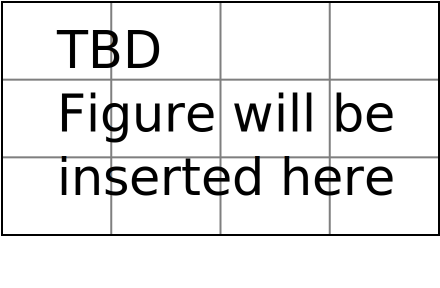
\includegraphics[width=0.8\textwidth]{fig/TBDFigure}
      \end{center}
      \caption{Hidden Markov Model}
      \label{fig:hmm}
   \end{figure*}

Formally, for some observed features $\Phi_r(x^s)$ of a note $x$ located in $s$th position of the phrase, and assume $\left[ \left[ y^t = \tau \right] \right]$ denotes the $t$th note is played at a velocity of $\tau$, the interaction of the two predicate can be written as 
%TODO hmm 3 formula 4
$$\phi^{st}_{r\sigma}(\mathbf{x}, \mathbf{y}) = \left[\left[y^t = \tau \right] \right]\Psi_r(x^s),\; 1\leq\gamma\leq d,\; \tau \in \Sigma $$

And for interaction between labels, the feature can be written as
%TODO hmm 3 formula 5
$$\hat{\phi}^{st}_{r\sigma}(\mathbf{x}, \mathbf{y}) = \left[\left[y^s = \sigma \wedge y^t = \tau \right] \right],\; \sigma, \tau \in \Sigma $$

By selecting a dependency order for the HMM model, we can restrict $s$'s and $t$'s. For example, for a first-order HMM, $s = t$ for the first feature, and $s = t-1$ for the second feature. The two features on the same time $t$ is then stacked into a vector $\Psi(x,y;t)$. The feature map for the whole sequence is simply the sum of all the feature vectors 

%TODO hmm 3 formula 6
$$\Phi(\mathbf{x}, \mathbf{y}) = \sum^T_{t=1}\Phi(\mathbf{x}, \mathbf{y};t)$$

Finally, the distance between two feature maps depends on the number of common label segments and the inner product between the input features sequence with common labels.


$$\langle\Phi(\mathbf{x}, \mathbf{y}), \Phi(\mathbf{\hat{x}}, \mathbf{\hat{y}})\rangle = \sum_{s,t}\left[\left[y^{s-1} = \hat{y}^{t-1}\wedge y^s = \hat{y}^t\right] \right] + \sum_{s,t}\left[\left[y^{s} = \hat{y}^{t}\right] \right]k(x^s, \hat{x}^t)$$


To speed up the computation of $F$ for HMM, a Viterbi-like decoding algorithm is used.


%TODO: how to define loss function for HMM?
%(2003) section 3
%ovserved output <--> tag
%previous tag <--> this tag (1-order markov)
% Psi = each note's above two property summed up
%similarity = same prev tag <--> this tag sequence + same tag <--> observed output distance

%Hard-margin one
%Soft-margin one => introduce slack variable 
%Example with large loss should be emphasized => slack rescaling
%Margin can also be scaled => margin rescaling
%There are too many constrains => greedy algo (2005), select a subset of constrains from the most violated constrains to solve
%To speed up, n-slack variables are reduced to 1-slack variable (2009)

%           \item Prediction error (risk):
%               $$R^\Delta_p(h) = \int_{\mathcal{X}\times\mathcal{Y}}\Delta(y, h(x)) dP(x,y)$$
%               \begin{tabular}{ll}
%                   where & $\Delta()$ is the loss function \footnote{Must satisfy $\Delta(x,x) = 0$, $\Delta(x,y) > 0$}\\
%                   & P(x,y) is the joint distribution of $\mathcal{X}$ and $\mathcal{Y}$
%               \end{tabular}

%    \begin{frame}{Emperical Risk}
%       \begin{itemize}
%           \item Emperical Risk from training sample $S$:\footnote{Emperical Risk Minimization Priciple (Vapnik V (1998) Statistical Learning Theory. Wiley, Chichester, GB)}

%               $$R^\Delta_S(h) = \frac{1}{n}\sum_{i=1}^{n}\Delta(y_i, h(x_i))$$
%                   where  $\Delta()$ is the loss function 

%           \item Classification SVM

%                   $$\displaystyle \min_{\mathbf{w}, \xi_i \geq 0} \frac{1}{2}\mathbf{w}^T\mathbf{w} + \frac{C}{n} \sum_{i=1}^{n} \xi_i$$
%                   s.t. $$\forall i\in {1,\cdots n}: y_i (\mathbf{w}^T x_i) \geq 1-\xi_i$$
                  

%           \item Learn a discriminant function $f:\mathcal{X} \times \mathcal{Y} \rightarrow \Re$ 
%           \item Given $x$, maximizing $f$ over all $y \in \mathcal{Y}$
%               $$h_\mathbf{w} (x) = \argmax_{y\in\mathcal{Y}} f_\mathbf{w} (x,y)$$
%           \item 
%               in which $$f_\mathbf{w} (x,y) = \mathbf{w}^T{\Psi}(x,y)$$
%               \begin{tabular}{ll}
%                   where & $\mathbf{w} \in \Re^N$ is a parameter vector\\
%                         & $\Psi(x,y)$ is a feature vector relating $x$ and $y$
%               \end{tabular}
              

 
% \section{Structural SVM}

% \section{Theoretical Details}
% %&=& &=& &=& &=& &=& &=& &=& &=& =
%    \begin{frame}{Lowest Risk}
%       \begin{itemize}
%           \item Prediction error (risk):
%               $$R^\Delta_p(h) = \int_{\mathcal{X}\times\mathcal{Y}}\Delta(y, h(x)) dP(x,y)$$
%               \begin{tabular}{ll}
%                   where & $\Delta()$ is the loss function \footnote{Must satisfy $\Delta(x,x) = 0$, $\Delta(x,y) > 0$}\\
%                   & P(x,y) is the joint distribution of $\mathcal{X}$ and $\mathcal{Y}$
%               \end{tabular}

%           %\item Training sample: $(x_1, y_1), (x_2, y_2), \cdots$ where $y_i$'s may have structural relationship
              
%       \end{itemize}
%    \end{frame}
%    \begin{frame}{Emperical Risk}
%       \begin{itemize}
%           \item Emperical Risk from training sample $S$:\footnote{Emperical Risk Minimization Priciple (Vapnik V (1998) Statistical Learning Theory. Wiley, Chichester, GB)}

%               $$R^\Delta_S(h) = \frac{1}{n}\sum_{i=1}^{n}\Delta(y_i, h(x_i))$$
%                   where  $\Delta()$ is the loss function 

%           %\item Training sample: $(x_1, y_1), (x_2, y_2), \cdots$ where $y_i$'s may have structural relationship
              
%       \end{itemize}
%    \end{frame}

%    \begin{frame}{Traditional SVM}
%       \begin{itemize}
%           \item Classification SVM

%                   $$\displaystyle \min_{\mathbf{w}, \xi_i \geq 0} \frac{1}{2}\mathbf{w}^T\mathbf{w} + \frac{C}{n} \sum_{i=1}^{n} \xi_i$$
%                   s.t. $$\forall i\in {1,\cdots n}: y_i (\mathbf{w}^T x_i) \geq 1-\xi_i$$
                  

              
%       \end{itemize}
%    \end{frame}

%    \begin{frame}{Structural SVM}
%       \begin{itemize}
%           \item Extend SVM for structural output
%           \item Learn a discriminant function $f:\mathcal{X} \times \mathcal{Y} \rightarrow \Re$ 
%           \item Given $x$, maximizing $f$ over all $y \in \mathcal{Y}$
%               $$h_\mathbf{w} (x) = \argmax_{y\in\mathcal{Y}} f_\mathbf{w} (x,y)$$
%           \item 
%               in which $$f_\mathbf{w} (x,y) = \mathbf{w}^T{\Psi}(x,y)$$
%               \begin{tabular}{ll}
%                   where & $\mathbf{w} \in \Re^N$ is a parameter vector\\
%                         & $\Psi(x,y)$ is a feature vector relating $x$ and $y$
%               \end{tabular}


                  

              
%       \end{itemize}
%    \end{frame}

%    \begin{frame}{N-slack Formulations}
%       \begin{itemize}
%           \item margin-rescaling: change hinge, fixing slope
%              $$\Delta_{MR}(y,h_\mathbf{w}) = \max_{\hat{y} \in \mathcal{Y}} \{ \Delta(y, \hat{y}) - \mathbf(x)^T {\Psi}(x,y) + \mathbf{w}^T{\Psi}(x,\hat{y}\} \geq \Delta(y,h_\mathbf{w}(x))$$
%           \item slack-rescaling: fixing hinge, changing slope
%              $$\Delta_{SR}(y,h_\mathbf{w}) = \max_{\hat{y} \in \mathcal{Y}} \{ \Delta(y, \hat{y}) (1 - \mathbf(x)^T {\Psi}(x,y) + \mathbf{w}^T{\Psi}(x,\hat{y} )\} \geq \Delta(y,h_\mathbf{w}(x))$$
              
%       \end{itemize}
%    \end{frame}

%    \begin{frame}{Optimization Problems}
%       \begin{itemize}
%           \item
%                $$\displaystyle \min_{\mathbf{w}, \xi_i \geq 0} \frac{1}{2}\mathbf{w}^T\mathbf{w} + \frac{C}{n} \sum_{i=1}^{n} \xi_i$$
%                s.t. for $i = 1\cdots n$
%           \item n-slack structural SVM w/ margin-rescaling
%                $$\forall \hat{y_i} \in \mathcal{Y}: \mathbf{w}^T[\Psi(x_i,y_i) - \Psi(x_i,\hat{y_i})] \geq \Delta(y_i, \hat{y_i}) - \xi_i $$

%           \item n-slack structural SVM w/ slack-rescaling
%                $$\forall \hat{y_i} \in \mathcal{Y}: \mathbf{w}^T[\Psi(x_i,y_i) - \Psi(x_i,\hat{y_i})] \geq 1 - \frac{\xi+i}{\Delta(y_i, \hat{y_i})}$$
%       \end{itemize}
%    \end{frame}

%    \begin{frame}{1-Slack Formulation}
%       \begin{itemize}
%           \item
%       \end{itemize}
%    \end{frame}


%TODO: theoratical background

\section{Implementation}
Thorsten Joachims from Cornell University created a good toolbox for SVM-HMM learning called $SVM^{hmm}$ \cite{Joachims2008}. According to the program's download page, the $SVM^{hmm}$ is an implementation of structural SVMs for sequence tagging \cite{TODO:altun2003} using the training algorithm described in \cite{TODO:tsoch2004, 2005} and \cite{TODO:Joachims et al. 2009}.The toolbox is contains two main program called \texttt{svm\_hmm\_learn} and \texttt{svm\_hmm\_classify}. The \texttt{svm\_hmm\_learn} takes a training file containing all the training sample. Each line in the training file is the featrues of a note, in the following format:
\begin{lstlisting}
	PERF qid:EXNUM FEAT1:FEAT1_VAL FEAT2:FEAT2_VAL ... #comment
\end{lstlisting}
\texttt{PERF} is the performance feature. The \texttt{EXNUM} after \texttt{qid:} identifies the phrases, all notes in a phrase will have the same \texttt{qid:EXNUM} identifier. Follwing the identifier are \texttt{feature name : feature value} pairs, separated by space. And anything after the \texttt{\#} is considered as comments.

      \begin{figure*}[tp]
         \begin{center}
            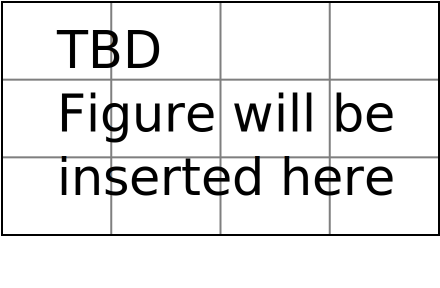
\includegraphics[width=\textwidth]{fig/TBDFigure}
         \end{center}
         \caption{Example input file} 
         \label{fig:expinput}
      \end{figure*}

For architectural simplicity, one model is trained for each performance feature. The input for a model is all the score features, and the model will predict a single performance feature. 


Because three performance features are used, three model file will be generated after running \texttt{svm\_hmm\_learn} on the 
\framebox{TODO: finish this section}


\subsection{Quantization}
One problem exist for using SVM-HMM on expressive performance: some of the features are continuous, but SVM-HMM can only generate discrete output label. Therefore quantization is required. 
%TODO: quantization
\framebox{TODO: finish quantization section}

\chapter{Corpus Preparation}
\label{chap:corpus}
  An expressive performance corpus is a set of performance samples. Since this research is based on a supervised learning algorithm, a high-quality corpus is essential to our success. Each sample consists of a score and its corresponding human recording. Some metadata such as phrasing, structure analysis, or harmonic analysis may also be included. In this chapter, we will review some of the existing corpora, specifications and formats of our corpus, and how we actually construct it.

\section{Existing Corpora} 
Unlike other research fields like speech processing or natural language processing, there exists virtually no publicly accessible corpus for computer expressive performance research. CrestMusePEDB \cite{crestmuse} (PEDB stands for "Performance Expression Database") is a corpus created by Japan Science and Technology Agency's CREST program. However, until the time of this writing, we cannot establish any contact with the database administrators to gain access to it. They claim to have a GUI tool for annotating the expressive performance parameters from audio recordings. Their repertoire covers many piano works from well-known classical composers like Bach, Mozart, and Chopin, and is recorded by world famous pianists. On their website \cite{crestmuse} they claim to contain the following data: PEDB-SCR - score text information, PEDB-DEV - performance deviation data and PEDB-IDX - audio performance credit. But the quality of the data is unknown.

Another example is the Magaloff Project \cite{magaloff}, which is created by some universities in Austria. They invited the Russian pianist Nikita Magaloff to record all solo works for piano by Frederic Chopin on a Bösendorfer SE computer-controlled grand piano. This corpus became the material for many subsequent researches \cite{Goebl2009, Grachten2011, Flossmann2009, Grachten2012, Flossmann2013, Flossman2011, Flossmann2010a}. Flossmann et al., one of the leading researchers of the project, also won the 2008 RenCon contest with a system based on this corpus called YQX \cite{yqx}. However, the corpus is not open up to the public. 

Since both corpora are not available, we need to implement our own. We will start by defining the specification.

\section{Corpus Specification}

The corpus we need must fulfill the following criteria:
\begin{enumerate}
   \item All the samples are monophonic, containing only a single melody without chords.
   \item No human errors, such as insertion, deletion, or wrong pitch exist in the recording; the score and recording are matched note-to-note.
   \item The phrasings are annotated by human. 
   \item The scores, recordings and phrasing data are in a machine-readable format.

   %\item The tempo label in MIDI recordings are the tempo by which the musician played. 
\end{enumerate}

Certain potentially useful information is not included because it is less relevant to our goal. Examples are:

\begin{enumerate}
   \item Advanced structural analysis, such as GTTM (Generative Theory of Tonal Music)\cite{GTTM}
   \item Harmonic analysis
   \item Piano pedal usage
   \item Piano fingerings
   \item Techniques of other musical instruments, such as violin pizzicato, tapping, or bow techniques.
   %\item Other instrument specific instructions, such as piano fingering, violin bow techniques etc.
\end{enumerate}

We choose Clementi's Sonatina Op.36 for our corpus. It is a must-learn repertoire for the piano students, so it is easy to find performers with a wide range of skill level to record the corpus. These sonatinas are in the Classical style, so the learned model can potentially be extended to other works from composers of the Classical era like Mozart and Haydn. There are six sonatinas included in Op.36. The first five have three movements each, and the last one has two movements. The movement titles and time signatures of all the pieces are listed in Table \ref{tab:cleminfo}


\begin{table}
   \centering
   \caption{Clementi's Sonatinas Op.36 }
   \label{tab:cleminfo}
   \begin{tabular}{lll}
      \hline
      \textbf{Title} & \textbf{Movement} & \textbf{Time Signature}\\
      \hline
      No.1 Sonatina in C major&    I. Allegro &4/4\\
      &    II. Andante &3/4\\
      &    III. Vivace &3/8\\
      No.2 Sonatina in G major&    I. Allegretto &2/4\\
      &    II. Allegretto &3/4\\
      &    III. Allegro &3/8\\
      No.3 Sonatina in C major&    I. Spiritoso &4/4\\
      &    II. Un poco adagio &2/2\\
      &    III. Allegro &2/4\\
      No.4 Sonatina in F major&    I. Con spirito &3/4\\
      &    II. Andante con espressione &2/4\\
      &    III. Rondó: Allegro vivace &2/4\\
      No.5 Sonatina in G major&    I. Presto &2/2\\
      &    II. Allegretto moderato &3/8\\
      &    III. Rondó: Allegro molto &2/4\\
      No.6 Sonatina in D major&    I. Allegro con spirito &4/4\\
      &   II. Allegretto   &6/8\\
      \hline
   \end{tabular}
\end{table}


 %we choose  for score to choose from, such as MusicXM \cite{Good2001}, LilyPon \cite{LilyPond}, Finale, Sibelius, ABC, MuseData, and Humdrum. The book \cite{Selfridge-Field1997} has a comprehensive review on this issue. %For research purpose, proprietary format like Finale and Sibelius is abandoned because of their limited support from open source tools. 
%To represent Clemetni's work in digital format, we choose MusicXML.
MusicXML is used to represent Clementi's work in digital format.
MusicXML is a digital score notation using XML (eXtensible Markup Language); it can express most traditional music notations and metadata. Most music notation softwares and software tools support the musicXML format. %An example snippet of a musicXML score is shown in Fig. \ref{fig:expxml}%LilyPond is a \LaTeX-like language for music typesetting. %ABC, MuseData and Humdrum are based on ASCII codes and each defines their unique representation for music score. 
%\begin{figure*}[tp]
%   \begin{center}
%      %TODO:Fig.:Example JSON code
%      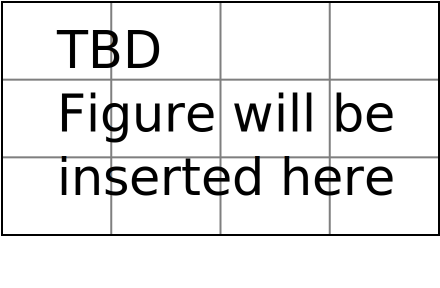
\includegraphics[width=\textwidth]{fig/TBDFigure}
%
%   \end{center}
%   \caption{Example MusicXML score}
%   \label{fig:expxml}
%\end{figure*}
%TODO: guitar pro?
Although MIDI is also a possible candidate for representing score, it is designed to hold instrument control signal rather than notation. Some music symbols may not be available in MIDI. Furthermore, MIDI represents music as a series of note-on and note-off events, which requires additional effort to transform them into the traditional notation.

But for representing the performance, MIDI is the most suitable format. Using a key-pressure-sensitive digital piano, the pianist can record in a natural way. The recordings will have a high precision in time, pitch and loudness (key pressure), and polyphonic tracks can easily be recorded separately. Although a WAV (Waveform Audio Format) audio recording has a higher fidelity than MIDI, it is harder to parse by computers. Without robust onset detection, pitch detection, and source separation technology, it is extremely difficult to extract the information. It takes unrealistic effor to manually annotate each WAV recordings, and the accuracy across different annotators may not be consistent. 

There is a way to keep both the score and the recording in one single MIDI file. Instead of recording the actual note-on and note-off timing, we keep the nominal note-on and note-off the same as in the score. Then, MIDI tempo-change events are inserted before each note to shift the performed timing of the recorded notes. Thus, the nominal time of each note represents the score, and the rendered time represents the performance. But since MIDI is so limited as a score format and it requires complex calculations to recover the performance, this method is not used in the research.
%A human musician can't play every note exactly on the beat, even if playing along with a metronome. There are two ways to record this behavior: first, record the exact note-on and note-off time, while keeping the tempo fixed; second, keep the notes on the beat, so the MIDI looks the same as the score. Then insert tempo-change event between each notes, so notes of the same length can be rendered differently because they have different tempo marker. The second method may look smart, because the score and performance can be stored in one MIDI file instead of two, but it would involve complex calculation when linearly scaling the tempo. Since tempos from different samples need to be normalized during feature extraction, the first method is superior  than the second.
%Other formats such as image files (scanned or typesetted by computer) or PDF files are an alternative, but they are not an option for direct computer analysis. 

%In this research, we use MusicXML as the main vehicle for music score, because of the following reasons: first, it covers most music notations and metadata need for this research. Second, it is supported in most music notation software, including the one used in this research -- MuseScore. Finally, the music21 toolbox can convert many other formats into MusicXML without problem.

Finally, we store the phrasing, which is the only metadata we used, in a plaintext file; each line in the phrasing file is the starting point of each phrase. The starting point is defined as the onset timing (in quarter notes) counted from the beginning of the piece\footnote{For a phrase that starts at a point which is a circulating decimal, for example $2\frac{1}{3}=2.333\cdots$, the starting point can be alternatively defined as any finite decimal between the end of the last phrase and the start of the current phrase. For example, if the last phrase stops at beat 1 and the second phrase start at $2\frac{1}{3}=2.333\cdots$ beat, the start point of the second phrase can be written as 2.3 or 2.0, etc.}. The phrasing is decided by the following principles: 
\begin{enumerate}
   \item Phrases may be separated by a salient pause.
   \item A phrase may end with a cadence.
   \item Phrases may be separated by dramatic change in tempo, key or loudness.
   \item Repeated structures may be repeated phrases.
\end{enumerate}
%The above criteria are just general principles, not strict rules, the phrasing is still decided subjectively.

%An automatic phrasing algorithm may be achieved in the future, either by fuzzy rules or by machine learning. With the automatic phrasing capability, the system can become fully automatic. But phrasing controls the structural expression of a piece, we left the phrasing decision to the user. Because we intend to leave some degree of freedom for users to expressive themselves. But note-level expression is too trivial to be assigned by hand, but deciding phrase-level expression is less demanding for an ordinary user. 
Since the phrasing controls the structural interpretation of a piece, we would like to leave this freedom for expression to the user. However, if there exists any good automatic phrasing algorithm, it can be easily integrated into the current system to make it full-automatic.

 
%\section{File Format}
\section{Implementation}

\subsection{Score Preparation}

The digital scores are downloaded from KernScore website \cite{KernScores}. The  scores are transformed into MusicXML from the original Hundrum file format (.krn) using the  music21 toolkit \cite{music21}. Because this research focuses on monophonic melodies only, the accompaniments are removed and the chords are reduced to their highest-pitched note, which is usually the most salient melody. The reduced scores are doubled-checked against a printed version publish by Durand \& Cie., Paris \cite{Clementi1915} to eliminate all errors. %We use MuseScore notation editor to view and edit MusicXML; some metadata errors are corrected by editing the MusicXML with text editors .

\subsection{MIDI Recording}
We have implemented two methods for recording: first, using a Yamaha digital piano to record MIDI; second, by tapping on a touch-sensitive device to express tempo, duration and loudness. Due to the accuracy consideration, only the recordings from the Yamaha digital piano are used in the expreiments.


We used a Yamaha P80 88-key graded hammer effect\footnote{Graded Hammer Effect feature provides a realistic key pressure response similar to a traditional acoustic piano.}digital piano for recording. Through a MIDI-to-USB converter, the keyboard was connected to Rosegarden Digital Audio Workstation (DAW) software on a Linux computer. The Rosegarden DAW also generated the metronome sound to help the performer maintain a steady speed. The metronome is mandatory because if the tempo is not assigned during the recording, the tempo information written in the MIDI file will be invalid, which makes subsequent parsing and linear scaling very difficult. So the performers were asked to follow the speed of the metronome, but they can adjust the metronome speed as they like, and apply any level of rubato as long as the overall tempo is steady. 

The second method, which is not used in the experiments, is to utilize touch-enabled input devices like a smartphone touchscreen or laptop touchpad. We have implemented an prototype using a Synaptics Touchpad on a Lenovo ThinkPad X200i laptop. When the user taps the touchpad once, one note from the score will be played, the duration and loudness will be controlled by the duration and pressure of the tapping action. The user can \enquote{play} the touchpad like a musical instrument. This idea has already been used in musical games and toys. This method is more user-friendly to general public because it requires minimal instrument skills and utilizes widely available hardwares. But most touchpad estimates pressure by finger contact area, so the accuracy in pressure is not very satisfying. But it is indeed a low-cost alternative to the MIDI digital piano.

\subsection{MIDI Cleaning and Phrase Splitting}
  After MIDIs are recorded, we use Python scripts to check if each recording is matched note-to-note with its corresponding score. If not, the mistakes are manually corrected. %For example, if the pitch was played wrongly, we will correct the pitch but keep the onset, duration  and intensity as is. 
  If there are small segments that are totally messed up, they will be reconstructed using repeated or similar segments from the same piece. The matched score and MIDI pairs are then split into phrases according to the corresponding phrasing file. The split phrases are checked once again for note-to-note match before they are put into experiments.

\section{Results}
Six graduate students (not majored in music) were invited to record the samples. The number of mistakes they made are listed in Table \ref{tab:mistakes}.\footnote{The performers are allowed to re-record as many time as they want, so the actual number of mistakes may be higher.} These mistakes are identified using the unix \texttt{diff}\cite{diff} tool. Five of them (A to E) finished Clementi's entire Op.36, while performer F only recorded part of the work. The total number of recordings and the corresponding phrase/note counts are shown in Table \ref{tab:corpuscount}. 

\begin{sidewaystable}[bp]
   \centering
   \caption{Number of mistakes in the corpus, blank cell means the performer did not record the piece}
   \label{tab:mistakes}
   \begin{tabular}{c|rrrrrrrrrrrrrrrrr|r}
      \hline
      Performer&1-1&1-2&1-3&2-1&2-2&2-3&3-1&3-2&3-3&4-1&4-2&4-3&5-1&5-2&5-3&6-1&6-2&Subtotal\\
      \hline
      A&0&5&2&4&3&0&4&2&2&4&5&9&9&2&3&4&1&59\\
      B&2&1&1&2&2&1&6&0&3&2&3&6&12&3&3&10&7&64\\
      C&1&1&0&1&0&1&2&0&0&3&2&3&10&1&35&6&1&67\\
      D&0&1&1&2&3&1&4&1&1&10&6&3&10&2&7&13&2&67\\
      E&2&3&4&4&0&3&4&0&0&21&6&22&23&3&9&18&13&135\\
      F&1&3&2&11&6&8&7&2&6&&15&&&&20&&&81\\
      \hline
      Subtotal&6&14&10&24&14&14&27&5&12&40&37&43&64&11&77&51&24&473\\
   \end{tabular}
\end{sidewaystable}
\begin{table}[bp]
   \centering
   \caption{Total recorded phrases and notes count}
   \label{tab:corpuscount}
   \begin{tabular}{l|rrr}
      \hline
      \bf Title&\bf Recordings&\bf Total Phrases&\bf Total Notes\\
      &\bf Count&&\\
      \hline
      No.1 Mov. I&6&72&1332\\
      No.1 Mov. II&6&60&882\\
      No.1 Mov. III&6&102&1566\\
      No.2 Mov. I&6&108&1920\\
      No.2 Mov. II&6&36&750\\
      No.2 Mov. III&6&168&2484\\
      No.3 Mov. I&6&156&3156\\
      No.3 Mov. II&6&42&444\\
      No.3 Mov. III&6&120&2628\\
      No.4 Mov. I&5&80&2325\\
      No.4 Mov. II&6&78&1332\\
      No.4 Mov. III&5&85&1920\\
      No.5 Mov. I&5&85&3360\\
      No.5 Mov. II&5&70&1580\\
      No.5 Mov. III&6&144&3384\\
      No.6 Mov. I&5&145&4180\\
      No.6 Mov. II&6&78&2754\\
      \hline
      Total&97&1629&35997\\
      \hline
   \end{tabular}
\end{table}

The number of phrases (according to our phrasing annotation) and notes are shown in Table \ref{tab:clemcount}. Fig. \ref{fig:notes} shows the length distribution of each movement; most movements have around a few hundred notes, except the long No.6 and some short second movements. Fig. \ref{fig:phrases} shows the length distribution in numbers of phrases; most movements are of around 20 phrases. The length distribution of the phrases in all six pieces are shown in Fig. \ref{fig:phrlength}: most phrases are shorter than 30 notes. Some very long phrases are usually virtuoso segments of very fast note passages, so it is hard to further split them.

\begin{table}[bp]
   \centering
   \caption{Phrases and notes count for Clementi's Sonatina Op.36}
   \label{tab:clemcount}
   \begin{tabular}{l|rr}
      \hline
      \textbf{Title}&\textbf{Phrases Count}&\textbf{Notes Count}\\
      \hline
      No.1 Mov. I&12&222\\
      No.1 Mov. II&10&147\\
      No.1 Mov. III&16&261\\
      No.2 Mov. I&18&320\\
      No.2 Mov. II&6&125\\
      No.2 Mov. III&28&414\\
      No.3 Mov. I&25&526\\
      No.3 Mov. II&6&74\\
      No.3 Mov. III&19&438\\
      No.4 Mov. I&25&465\\
      No.4 Mov. II&12&222\\
      No.4 Mov. III&16&384\\
      No.5 Mov. I&17&672\\
      No.5 Mov. II&13&316\\
      No.5 Mov. III&24&564\\
      No.6 Mov. I&28&836\\
      No.6 Mov. II&11&459\\
      \hline
      \textbf{Total} &286&6445\\
      \hline
   \end{tabular}
\end{table}


\begin{figure*}[tp]
   \begin{center}
      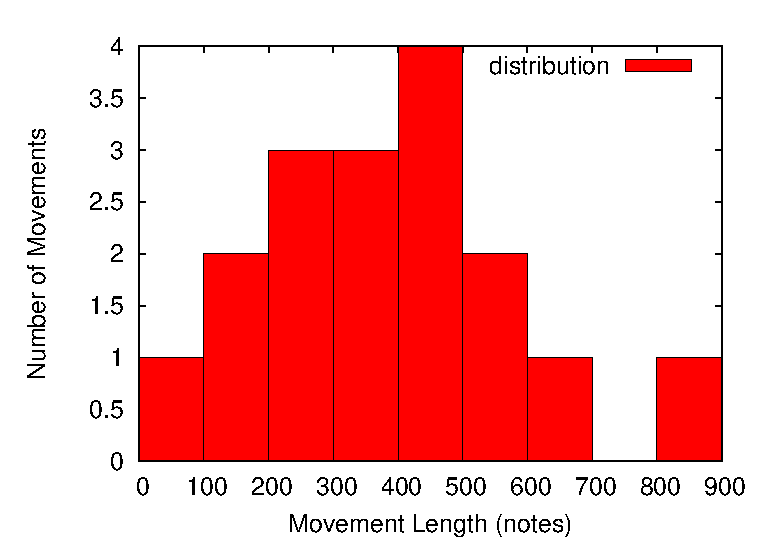
\includegraphics[width=\textwidth]{fig/notes}

   \end{center}
   \caption{Movement length (notes) distribution}
   \label{fig:notes}
\end{figure*}

\begin{figure*}[tp]
   \begin{center}
      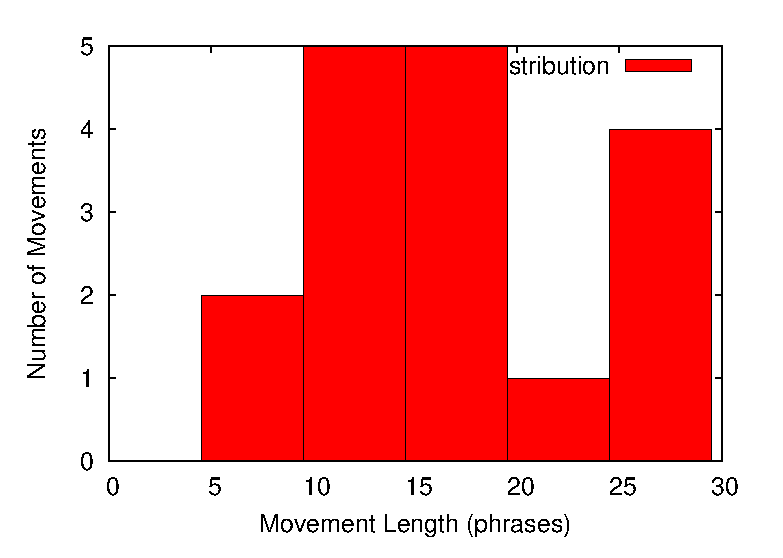
\includegraphics[width=\textwidth]{fig/phrases}

   \end{center}
   \caption{Movement length (phrases) distribution}
   \label{fig:phrases}
\end{figure*}

\begin{figure*}[tp]
   \begin{center}
      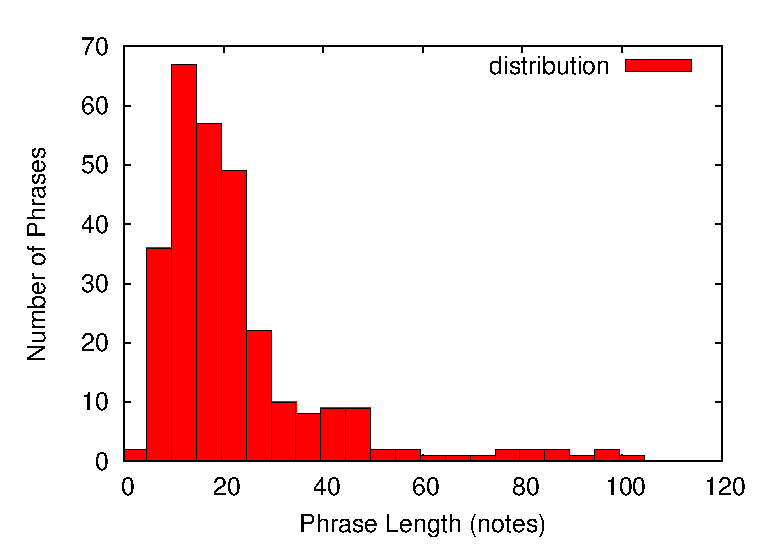
\includegraphics[width=\textwidth]{fig/phrlength}

   \end{center}
   \caption{Phrase length (notes) distribution}
   \label{fig:phrlength}
\end{figure*}






 %TODO:recording example pic
%\framebox{TODO:mention Fig. \ref{fig:exprecording}}
%\begin{figure*}[tp]
%   \begin{center}
%      %TODO:Fig.:Example JSON code
%      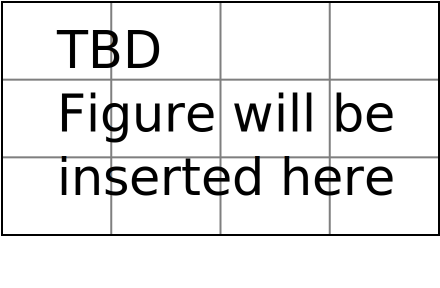
\includegraphics[width=\textwidth]{fig/TBDFigure}
%
%   \end{center}
%   \caption{Example Recording Compared to Score (Pianoroll)}
%   \label{fig:exprecording}
%\end{figure*}
%\framebox{TODO:error count}

%\framebox{REVIEW1}

\chapter{Experiments and Results}
\section{Onset Timing Normalization Selection}
\subsection{Experiment Design}
In section \ref{TODO:feature section}, four nomalization method is proposed. To see which one is most robust, we validated them with emprical data. A robust normalization method should produce a mean-reverse sequence, not a monotonic increase or decrease sequence. Four types of nomalization method is applied to every samples in the corpus, the result is shown in Figure \ref{fig:normalize_result} A regression analysis was applied to the result to see if there are clear trend in the normalized value.
\subsection{Results}

\section{Parameter Selection}
\subsection{Experiment Design}
Structural Support Vector Machine has some parameters that needed to be adjusted. We will leave the others to the defaults and change the SVM C trad-off parameter in this experiment. Since three models are learned for three performance features, we have three parameters to adjust. 
%TODO default parameters

[TODO: phrases count] phrases from [TODO:song counts] songs are used for training. Every first, fifth, and tenth phrases from each song is not included in the training sample, but used as testing samples. A three-by-three grid is layed out for three C parameters, each C takes the value of the powers of tenfrom [TODO: Cs] $10^{-5}$ to $10^4$, so [TODO: num of experiment] paramenters are tested. Then the result is validated
\begin{enumerate}
	\item Are all the output samples successfuly generated? (Generation may fail if the performance features are unreasonable, for example, negative onset timeing.)
	\item Is the order of the notes preserved? Sometimes the first note is delayed too long and the second note is played too early, so the order is swaped.
	\item Are there any extreme parameters that makes the expressive performance unnatural?
\end{enumerate}

The first two criterias are checked by python scripts, the last one is done by manual inspection.


\subsection{Results}
\section{Turing Test}
\subsection{Experiment Design}

\subsection{Results}

\chapter{Conclusions}
We have created a system that can perform monophonic score expressively. The expressive performance knowledge is learned from hum an recording using structural support vector machine with hidden Markov model output (SVM-HMM). We have also created a corpus consisting of scores and MIDI recordings.  From subjective test, we find that the computer generated performance still can't achieve the same level of expressiveness of human performers. However, from our similarity measure, the computer generated expressive performance are much similar to the human performance than inexpressive MIDI. %we show that although the amateur and professional musician can still differentiate the generated performance from human recordings, test subjects with no music background are giving equal ratings to the generated performance and human recordings, which means our system has the same expressive power as human.

There are many room for improvement. Structural expressions such as phrasing, contrast between sections, or even contrast between movements can be added, which requires automatic structural analysis. Other information like text notations, harmonic analysis and other musicological analysis can be added to the learning process. More subtle musical expressions like rhythm and pulse can potentially be automatically analyzed. Supporting homophonic or polyphonic music is also important for the system to be useful. Sub-note expressions like physical model synthesizer or envelope shaping can also be applied to generate performances for specific musical instruments. It's also crucial to test the system on more samples of different genre or music style. We also believe that combining rule-based model and machine-learning model may be a possible direction for computer expressive music performance research. With rules serving as a high level guideline for structural expression, the machine-learning model can focus on note or sub-note level expression. User can gain more control by tweaking the rules.
%\framebox{TODO:error model}


%TODO: structure
%TODO Expert system
%TODO Model selection
%TODO Jazz style
%TODO


%\chapter{Theory of surface plasmon polaritons in metallic nano-structures}
\label{c:thm}
\section{Definition of plasmon}

Plasmon is collective oscillation of conduction electron gas, a quasi-particle resulting from the quantization of plasma oscillations just like phonons are quantizations of mechanical vibrations. The simplest case is the volume plasmon as shown in Figure~\ref{fig:bulk}.
\begin{figure}[htb]
\centering
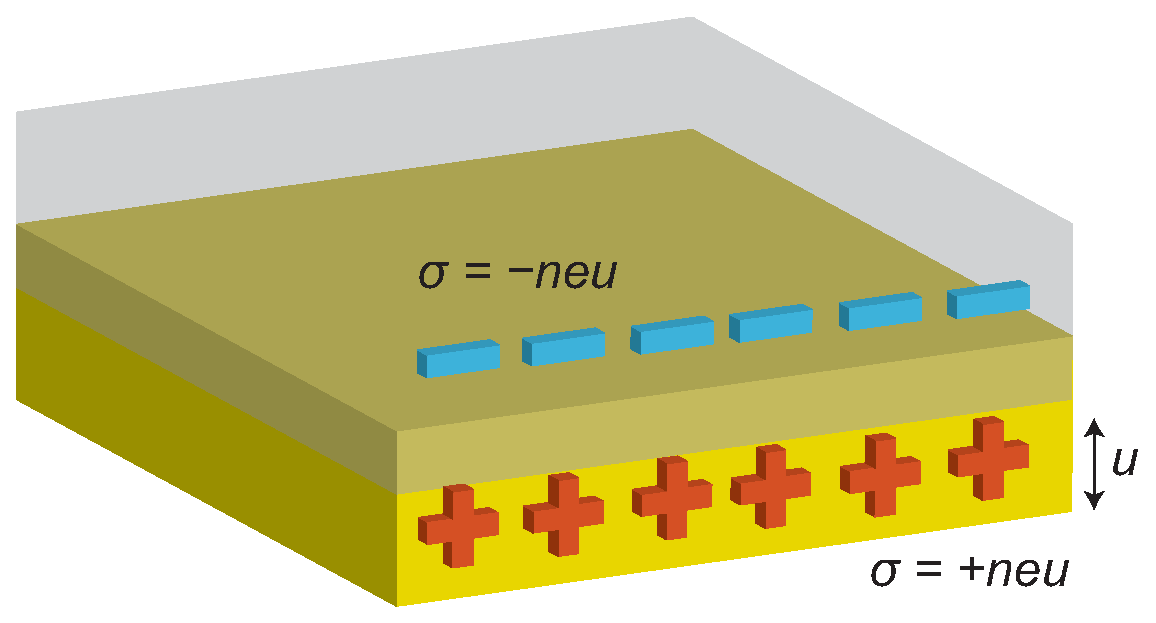
\includegraphics[scale=0.5]{THM/bulk.eps}
\caption{\label{fig:bulk}Longitudinal collective oscillations of the conduction electrons of a metal (Volume plasmons)}
\end{figure}
 We can derive plasma frequency $\omega_p$ from the simple harmonics oscillation model, a collective displacement of the electron cloud by a distance $u$ leads to a surface charge density $\sigma = \pm neu$ at the slab boundaries. This establishes a homogeneous electric field $\mathbf{E} = \frac{neu}{\varepsilon_0}$ inside the slab. Thus, the displaced electrons experience a restoring force, and their movement can be described by the equation of motion $nm\ddot{u} = -ne\mathbf{E}$. Inserting the expression for the electric field, this leads to
 \begin{subequations}
 \begin{align}
 nm\ddot{u} = -\frac{n^2e^2u}{\varepsilon_0} \\
 \ddot{u} + {\omega_p}^{2}u = 0\text{.}
 \end{align}
 \end{subequations}
  The plasma frequency $\omega_p = \sqrt{\frac{ne^2}{\varepsilon_0m}}$ can thus be recognized as the natural frequency of a free oscillation of the electron sea. The quanta of these charge oscillations are called plasmons. Due to the longitudinal nature of the excitation, volume plasmons do not couple to transverse electromagnetic waves, and can only be excited by particle impact. We can derive the dispersion relation of the generalization of volume plasmons, traveling plasma waves, from curl electric field equations (Equations~\ref{eq:curlE})
 \begin{subequations}
 \begin{align}
 \curl{\curl \mathbf{E}} &= -\mu_0 \frac{\partial^2\mathbf{D}}{\partial t^2}\label{eq:curlE}\\
\mathbf{K}( \mathbf{K}\cdot \mathbf{E}-K^{ 2 }\mathbf{E} ) &=-\varepsilon ( \mathbf{K},\omega  ) \frac { { \omega  }^{ 2 } }{ { c }^{ 2 } } \mathbf{E}
 \end{align}
 \end{subequations}  
and plasma model, and a simple equation of motion for an electron of the plasma subjected to an external electric field $\mathbf{E}$
 \begin{equation}
m\ddot{\mathbf{x}} + m\gamma\dot{\mathbf{x}} = -e\mathbf{E}\text{.}
\end{equation}
Assuming a harmonic time dependence $\mathbf{E}( t )=\mathbf{E}_0\mathrm{e}^{-i\omega t}$ of the driving field, a particular solution of this equation describing the oscillation of the electron is $\mathbf{x} ( t ) = \mathbf{x}_0 \mathrm{e}^{-i\omega t} $. The complex amplitude $\mathbf{x}_0$ incorporates any phase shifts between driving field and response via
\begin{equation}
\mathbf{x} ( t ) = \frac{e}{m( \omega^2 + i\gamma\omega )}\mathbf{E}( t )\text{.}
\end{equation}
The displaced electrons contribute to the macroscopic polarization
\begin{equation}
\mathbf{P}=-\frac{ne^2}{m( \omega^2 + i\gamma\omega )}\mathbf{E}( t )\text{.}
\end{equation}
Inserting $\mathbf{P}$ into dielectric displacement field equation $\mathbf{D} = \varepsilon_0\mathbf{E} + \mathbf{P}$ yields
\begin{equation}
\mathbf{D} = \varepsilon_0(1-\frac{\omega_p^2}{\omega^2 + i\gamma\omega})\mathbf{E}\text{,}
\end{equation}
where $\omega_p^2 = \frac{ne^2}{\varepsilon_0m}$. Therefore, the dielectric function of the free electron gas
\begin{equation}
\varepsilon(\omega) = 1- \frac{\omega_p^2}{\omega^2 + i\gamma\omega}\text{.}\label{eq:dielefu}
\end{equation}
We arrive at the desired result by using equation~\ref{eq:dielefu} and the generic dispersion relation $K^2=\varepsilon(\mathbf{K},\omega)\frac{\omega^2}{c^2}$, the dispersion relation of traveling waves becomes
\begin{equation}
\omega^2 = \omega_p^2 + \mathbf{K}^2c^2\text{.}
\end{equation}
From this relation, we can figure out the oscillation properties in any frequency of external field. Note that this branch can not confine the electromagnetic waves, it would radiate out the energy, so this mode is also called radiative surface plasmon.

\section{Surface plasmon polaritons at interface between dielectric and metal}

Surface plasmon polaritons (SPPs) are eigenmodes of transverse magnetic (TM) waves, which coupling the electromagnetic fields to oscillations of the conductor's electron plasma, propagate at a interface between dielectric and metal, and are confined in perpendicular direction. Providing a flat interface between dielectric and metal half-spaces with dielectric constants $\varepsilon_d$ and $\varepsilon_m$ , respectively, and assuming the interface normal to z direction and the SPPs propagate along the $x$ direction, the SPP wave vector $\beta$ is related to the frequency $\omega$ through the dispersion relation
\begin{equation}
\beta = k_0\sqrt{\frac{\varepsilon_d\varepsilon_m}{\varepsilon_d + \varepsilon_m}}\text{,}\label{eq:sppsdisp}
\end{equation}
where $k_0 = \omega/c$ is the free-space wave vector. We take $\omega$ to be real and allow $\beta$ to be complex.

The optical response of metals is often described by the Drude model for a free-electron gas~\cite{kittel1976introduction},
\begin{equation}
\varepsilon_{Drude}(\omega)=1-\frac{\omega_p^2}{\omega^2+i\Gamma\omega}\text{,}
\end{equation}
in which $\Gamma$ is a damping rate due to electron-electron and electron-phonon scattering.
Figure~\ref{fig:SPPdisp} shows the dispersion curve~\ref{eq:sppsdisp} with Drude metal  in the absence of losses ($\Gamma=0$) for air ($\varepsilon_d = 1$) and fused silica ($\varepsilon_d = 2.25$) interface.
\begin{figure}[htb]
\centering
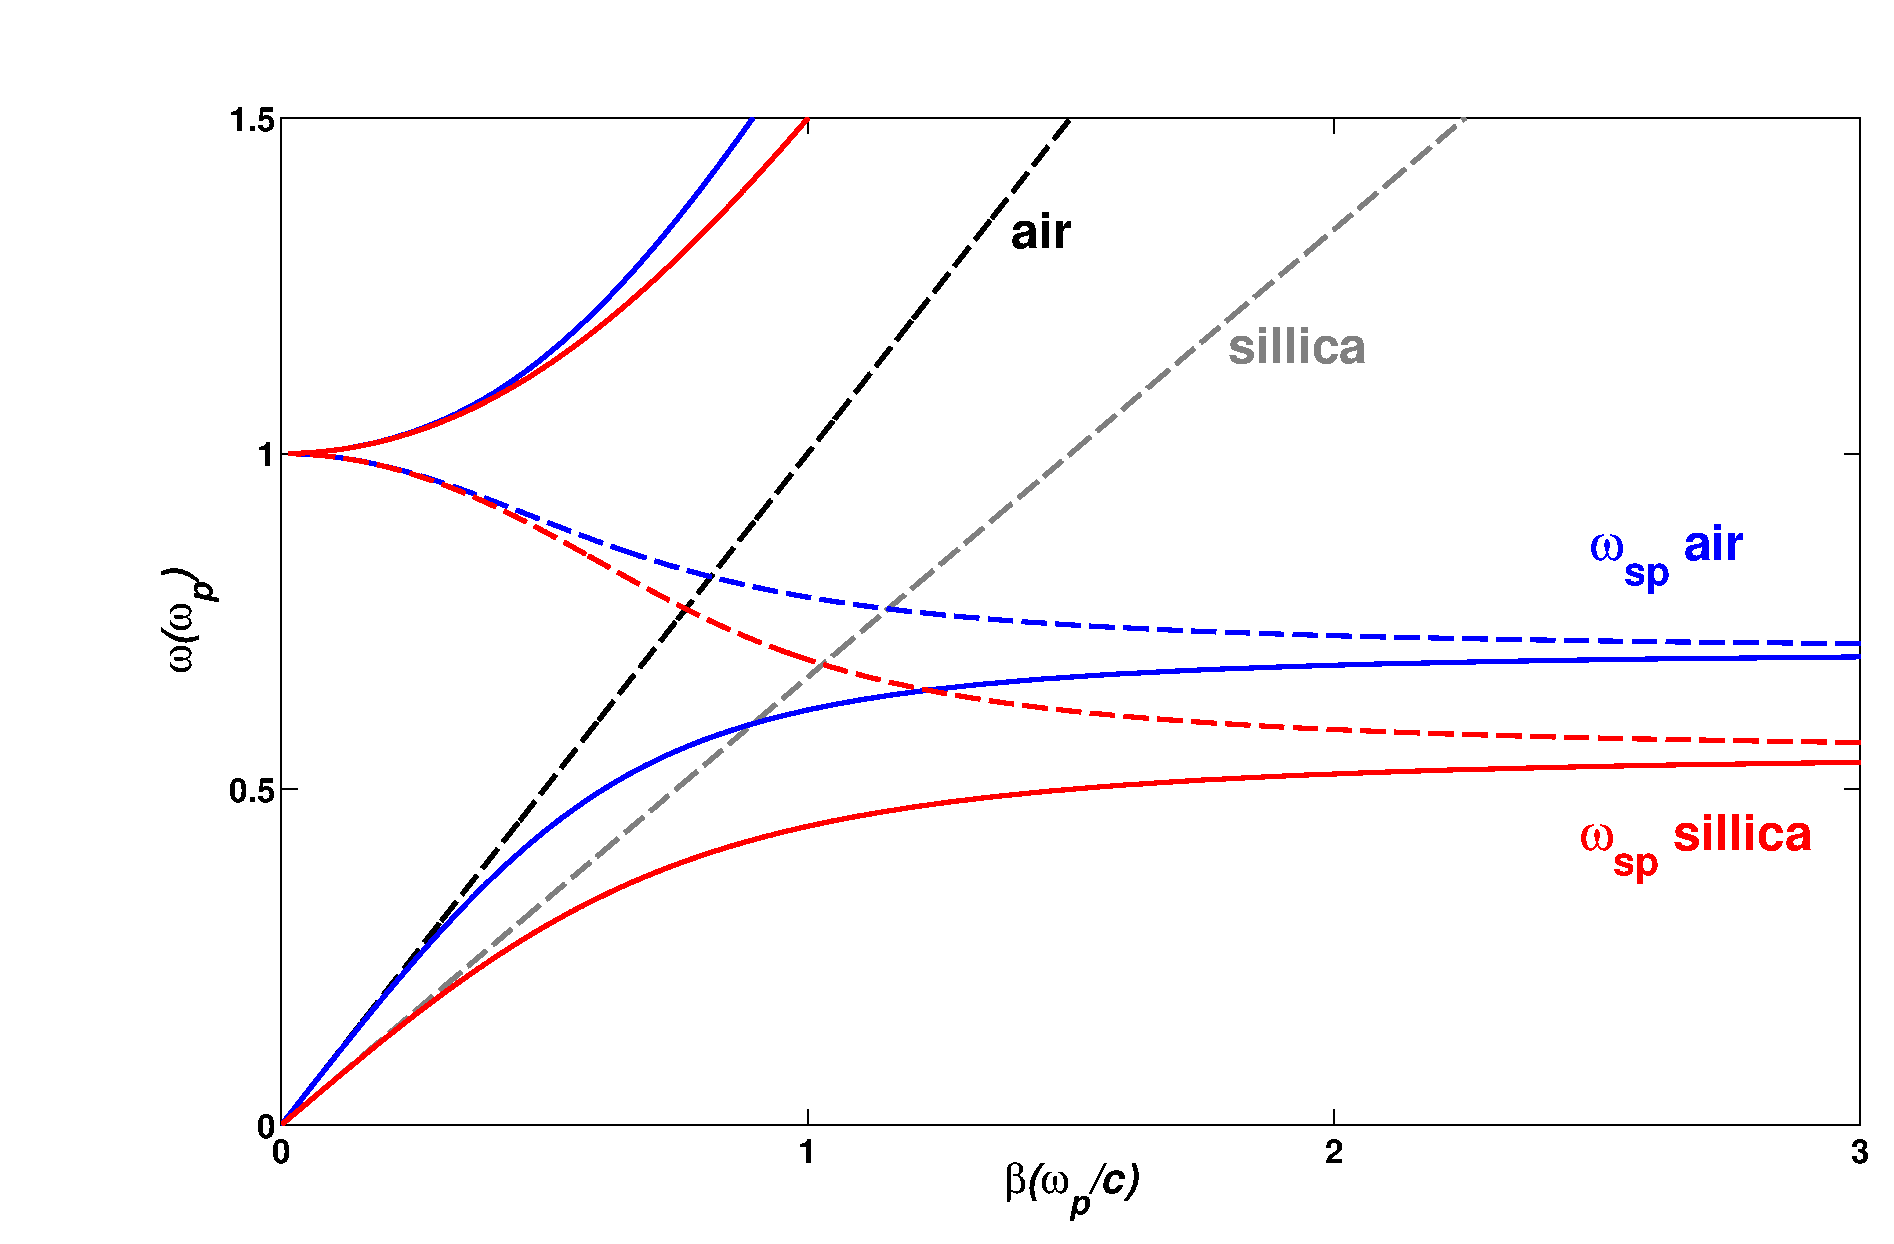
\includegraphics[scale=0.4]{THM/SPPdisp.eps}
\caption{\label{fig:SPPdisp}Dispersion relation of SPPs at the interface between a Drude metal with negligible collision frequency and air (blue curves) and silica (red curves).}
\end{figure}
For small wave vectors SPPs propagation constant $\beta$ is close to $k_0$ at the light line, in the opposite regime of the frequency close to surface plasmon frequency $\omega_p$. It also shows that the SPPs line lying to the right of the respective light lines of air and silica, so that SPPs are directed by light due to phase mismatching. The wave vector mismatch between SPPs and radiation modes needs to be overcome in order to excite or detect SPPs. This can be achieved by multiple methods~\cite{raether1988surface}. In the Otto configuration, light in a prism that is brought in close vicinity to a metal surface can excite SPPs through coupling to the evanescent field. Because light in the prism has a larger wave vector than that in air, it can be phase-matched to the SPPs. In the related Kretschmann-Raether geometry, coupling to SPPs occurs through a metal film that is deposited on a prism. In the grating coupling configuration, metal surface with a shallow grating of grooves or holes with lattice constant $a$. For the simple 1D grating of grooves depicted in Figure~\ref{fig:grating},
\begin{figure}[htb]
\centering
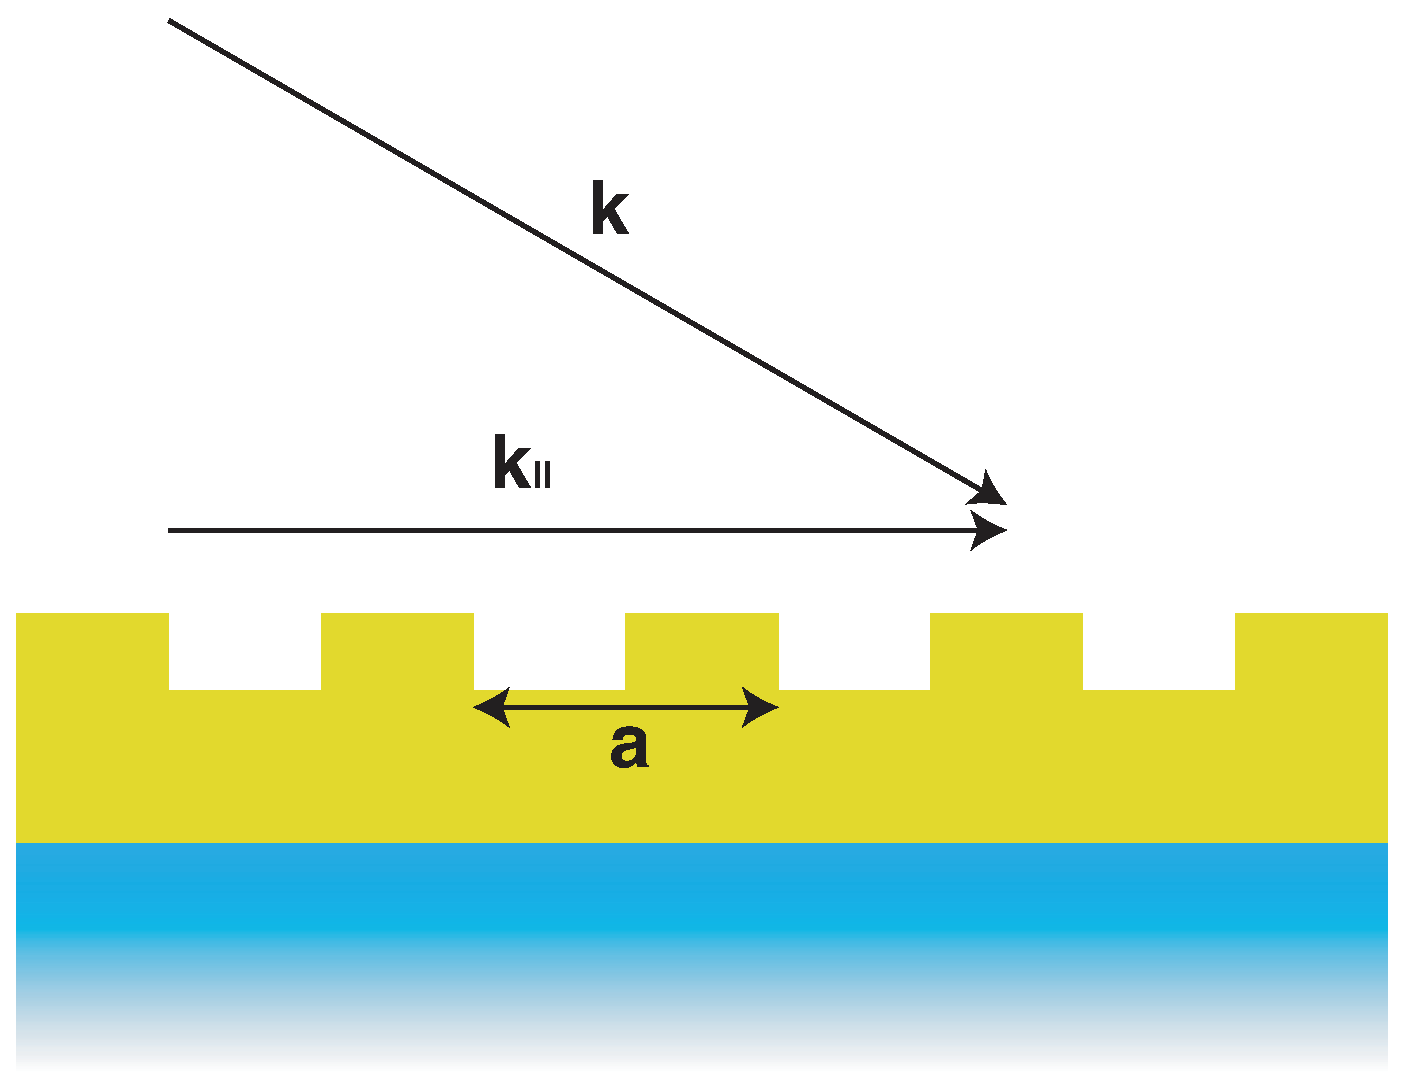
\includegraphics[scale=0.5]{THM/grating.eps}
\caption{\label{fig:grating}Phase-matching of light to SPPs the grating coupling configuration.}
\end{figure}
phase-matching takes place when the condition is fulfilled
\begin{equation}
\beta = k_0 \sin{\theta} \pm \nu g\text{,}
\end{equation}
where $g=\frac{2\pi}{a}$ is the reciprocal vector of the grating, and $\nu=(1,2,3\dots)$.
As with prism coupling, excitation of SPPs is detected as a minimum in the reflected light. The reverse process can also take place, SPPs propagating along a surface modulated with a grating can couple to light and thus radiate. 

%\bibliographystyle{unsrt}
%\bibliography{thesisbib}
%\chapter{Experiment}
\label{c:exp}

\section{Atomic force microscopy}

\begin{figure}[htb]
\centering
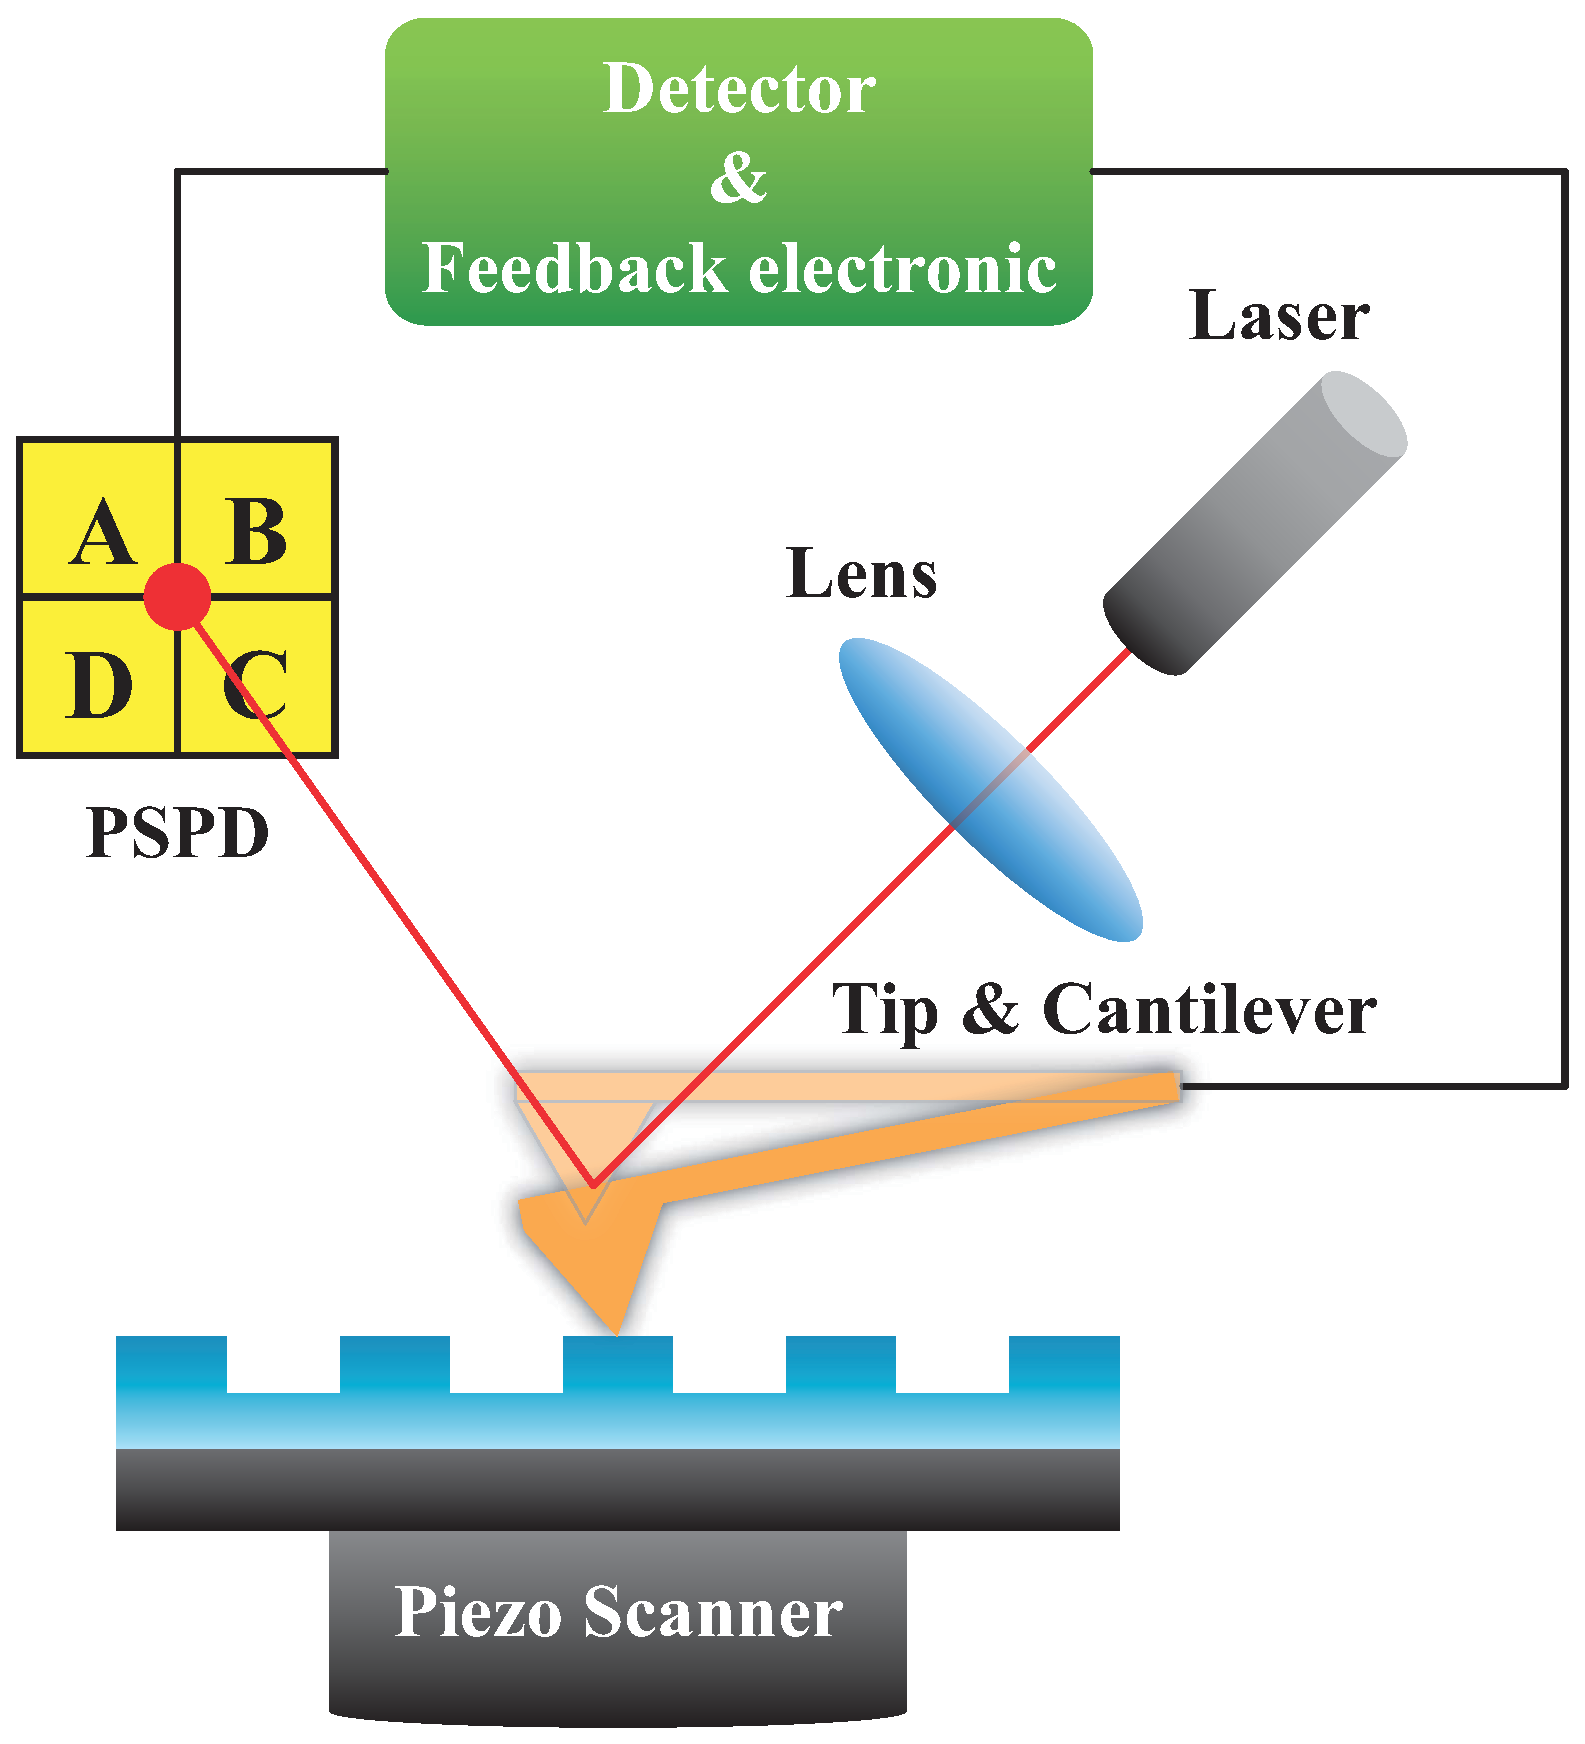
\includegraphics[scale=0.35]{EXP/afm1.eps}
\caption{\label{fig:afm1}Schematic of atomic force microscopy.}
\end{figure}
Atomic force microscope (AFM) is a type of scanning probe microscopes (SPM)~\cite{bennig1988atomic}.  The schematic of AFM is shown in Figure~\ref{fig:afm1}. AFM operates by measuring force between a probe and the specimen surfaces. In general,  the probe is a sharp tip at a cantilever's end. The cantilever can be deflected by atomic forces to sufficiently large amount, then AFM can measure the vertical and lateral deflections of the cantilever by using the optical system. A laser beam is transmitted to cantilever, and the reflected laser beam is detected with a position-sensitive photo detector (PSPD). PSPD is four-sectional that allows measuring not only vertical but lateral bending too(Figure~\ref{fig:afm2}). The output of the PSPD is provided to a computer for processing of the data for providing a topographical image of the surface with atomic resolution, and controlling the height between probe and specimen surfaces by applying voltage on piezoelectric scanner.
\begin{figure}[htb]
\centering
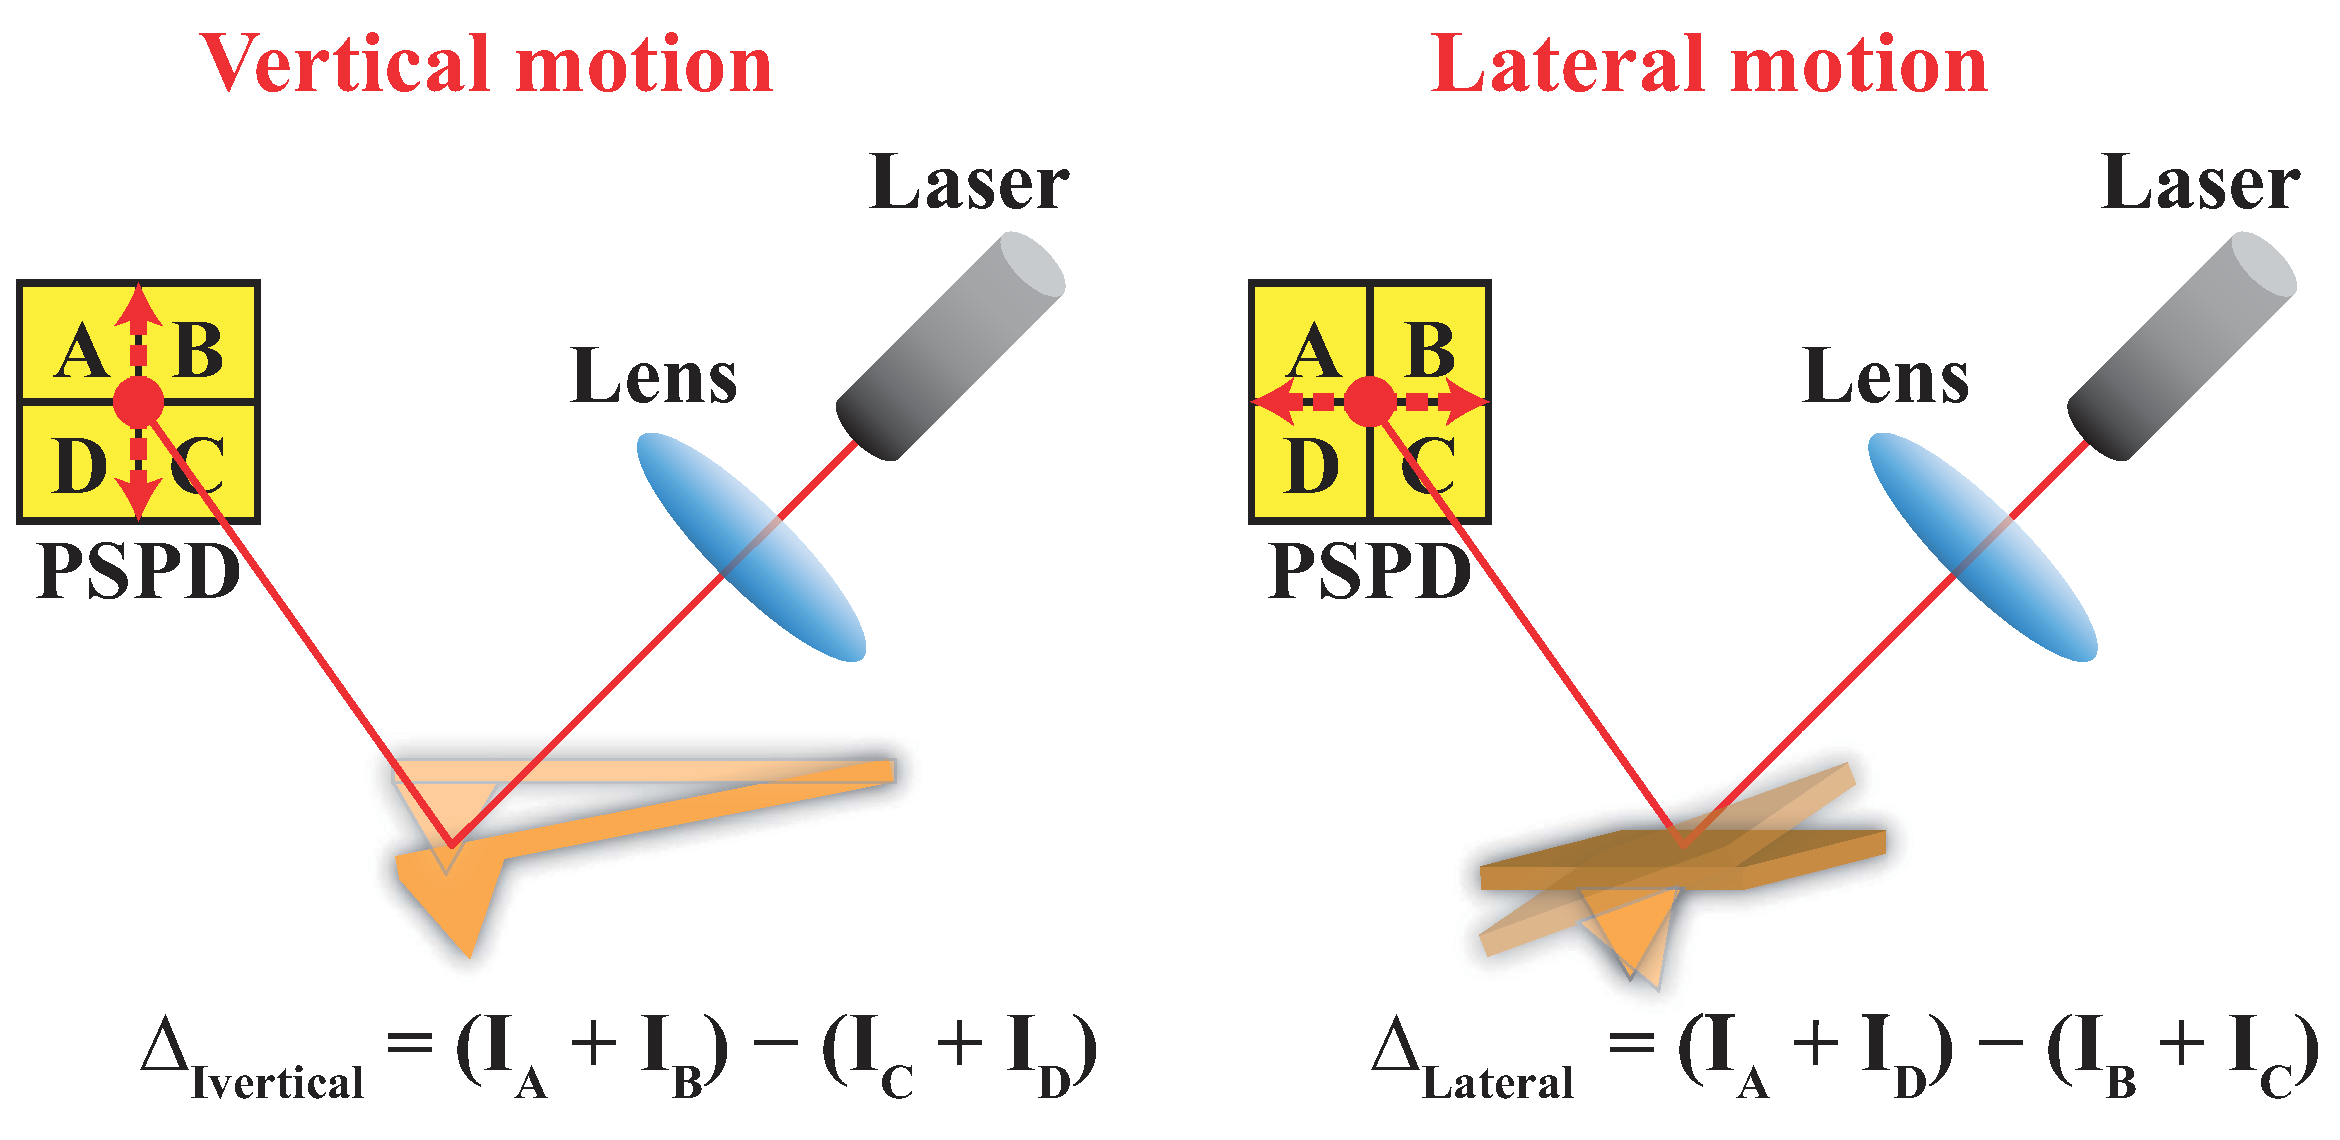
\includegraphics[scale=0.4]{EXP/afm2.eps}
\caption{\label{fig:afm2}Schematic of optical system for cantilever deflections detection.}
\end{figure}

The physical principle of the AFM operation is based on interaction between the probe tip and the specimen surface(Figure~\ref{fig:afm3}). When the cantilever approaches the specimen surface, Van der Waals forces start acting upon it . They are sufficiently far-ranging and are felt at the distance of a few tens of angstroms. Then at the distance of several angstroms repulsive force starts acting. In humid air a water layer is present on the specimen surface. The capillary force arises that holds the tip in contact with the surface and increases the minimum achievable interaction force. Electrostatic interaction between the probe and the sample may appear rather often. This can be both attraction and repulsion. Van der Waals attraction forces, capillary, electrostatic and repulsion forces at the point where the tip touches the sample and forces acting upon the tip from the deformed cantilever compensate each other in equilibrium. Based on the type and degree of this interaction the AFM modes can be broken down into contact and semi-contact(Figure~\ref{fig:afm3} ), which is a transition mode between the contact and non-contact modes.
\begin{figure}[htb]
\centering
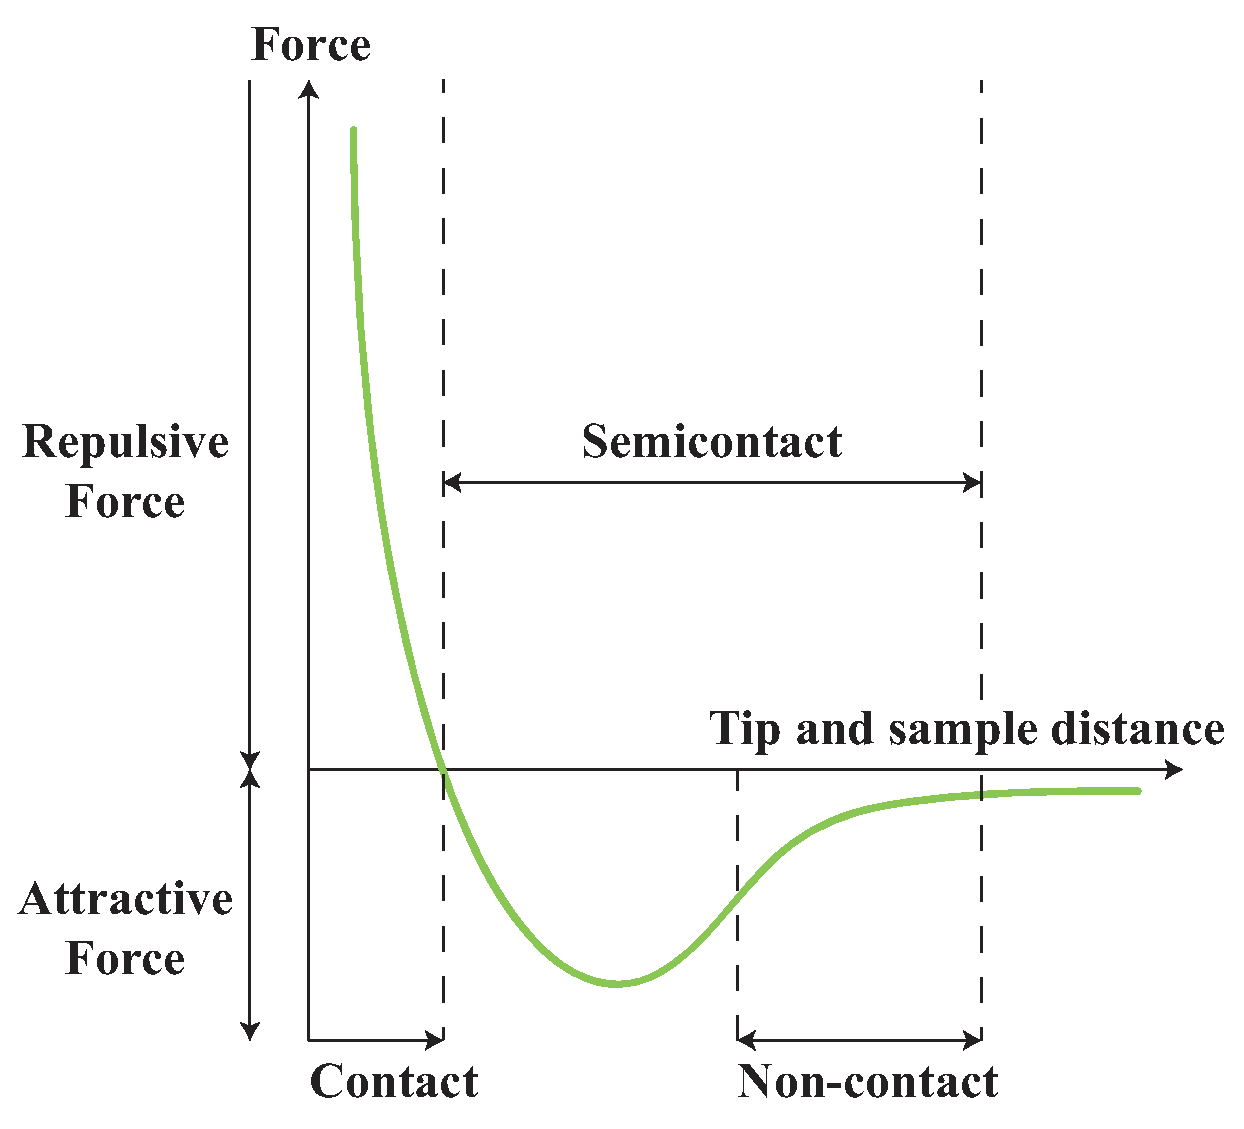
\includegraphics[scale=0.6]{EXP/afm3.eps}
\caption{\label{fig:afm3}Sketch of tip-sample forces.}
\end{figure}

\paragraph{Contact mode}

In contact mode of operation the cantilever deflection under scanning reflects repulsive force acting upon the tip. Repulsion force $\mathbf{F}$ acting upon the tip is related to the cantilever deflection value $\mathbf{x}$ under Hooke's law: $\mathbf{F}=-K \cdot  \mathbf{x}$, where $K$ is cantilever spring constant. The spring constant values for different cantilevers usually vary from 0.01 to several $\mathbf{N/m}$.

In our units the vertical cantilever deflection value is measured by means of the optical registration system and converted into electrical signal DFL (difference signal between the upper and lower halves of the PSPD) . In contact mode the DFL signal is used as a parameter characterizing the interaction force between the tip and the surface. There is a linear relationship between the DFL value and the force. In constant force mode of operation the deflection of the cantilever is maintained by the feedback circuitry on the preset value. So vertical displacement of the scanner under scanning reflects topography of sample under investigation.

Contact force microscopy is surface topography measurement in the contact mode.The microscope operation in the mode of maintaining constant interaction force between the tip and the surface sample, and is the base for measuring surface topography as well as for measuring local rigidity, local viscosity and local friction force. Constant force mode has some advantages and disadvantages. Main advantage of constant force mode is possible to measure with high resolution simultaneously with topography and some other characteristics, such as friction forces, spreading resistance etc. Constant force mode has also some disadvantages. Speed of scanning is restricted by the response time of feedback system. When exploring soft samples they can be destroyed by the scratching because the probe scanning tip is in direct contact with the surface. Therefore, under scanning soft unhomogeneous samples the local flexure of sample surface varies. As a result acquired topography of the sample can be proved distorted. Possible existence of substantial capillary forces imposed by a liquid adsorption layer can decrease the resolution.

\paragraph{Semi-contact mode}

The semi-contac mode can be characterized by some advantages in comparison with contact mode. First of all, in this mode the force of pressure of the cantilever onto the surface is less, that allows to work with softer materials such as polymers and bio-organics. The semi contact mode is also more sensitive to the interaction with the surface that gives a possibility to investigate some characteristics of the surface distribution of magnetic and electric domains, elasticity and viscosity of the surface. 

Widely used semi-contact mode has some disadvantage concerned with the usage of the feedback circuit. The scanning speed in semi-contact mode is restricted by the feedback circuit reaction time. This disadvantage can be overcome by the fact that under scanning new value of cantilever oscillation amplitude (and error signal) usually is achieved faster than preset value of the cantilever oscillation amplitude can be reached by the feedback system. Time of the reaching new value of the oscillation amplitude is determined by the oscillation period and Q-quality of the cantilever.
The feedback error signal, emerging when scanning in the semi-contact mode, contains some additional information about the topography. It can be utilized for achieving a more precise recovery of the relief. 

Additionally, similarly to the contact error mode, which can be considered as intermediate between the constant force mode and constant height mode, the feedback gain factor (i.e. the feedback processing speed) can be adjusted for the system to be able to trace subtle changes of the relief and to be too slow to trace the steep changes. Then, when the probe travels over minor irregularities, scanning will be carried out with an almost constant piezo scanner length. As a result, the slow changes of the relief will hardly show up on the images, and the steep changes will appear in high contrast. This may be helpful in finding minor irregularities on large areas against major sloping relief features. It must be noted that height of the minor irregularities must be less than amplitude of cantilever oscillation.

\section{Scanning electron microscopy}

The scanning electron microscope (SEM) is used for the observation of specimen surfaces~\cite{von1938elektronen}. When the specimen is irradiated with a fine electron beam, secondary electrons are emitted from the specimen surface. Topography of the surface can be observed by two-dimensional scanning of the electron probe over the surface and acquisition of an image from the detected secondary electrons. The concept schematic of commercial SEM (JEOL, JSM-6500F) is shown in Figure~\ref{fig:sem1}. The basic unit is composed of an electron optical system, a specimen stage, a secondary-electron detector, an image display unit, and an operation system. The electron optical system consists of an electron gun, a condenser lens and an objective lens to produce an electron probe, a scanning coil to scan the electron probe, and other components. The system inside of the microscope column are kept at vacuum.
\begin{figure}[htb]
\centering
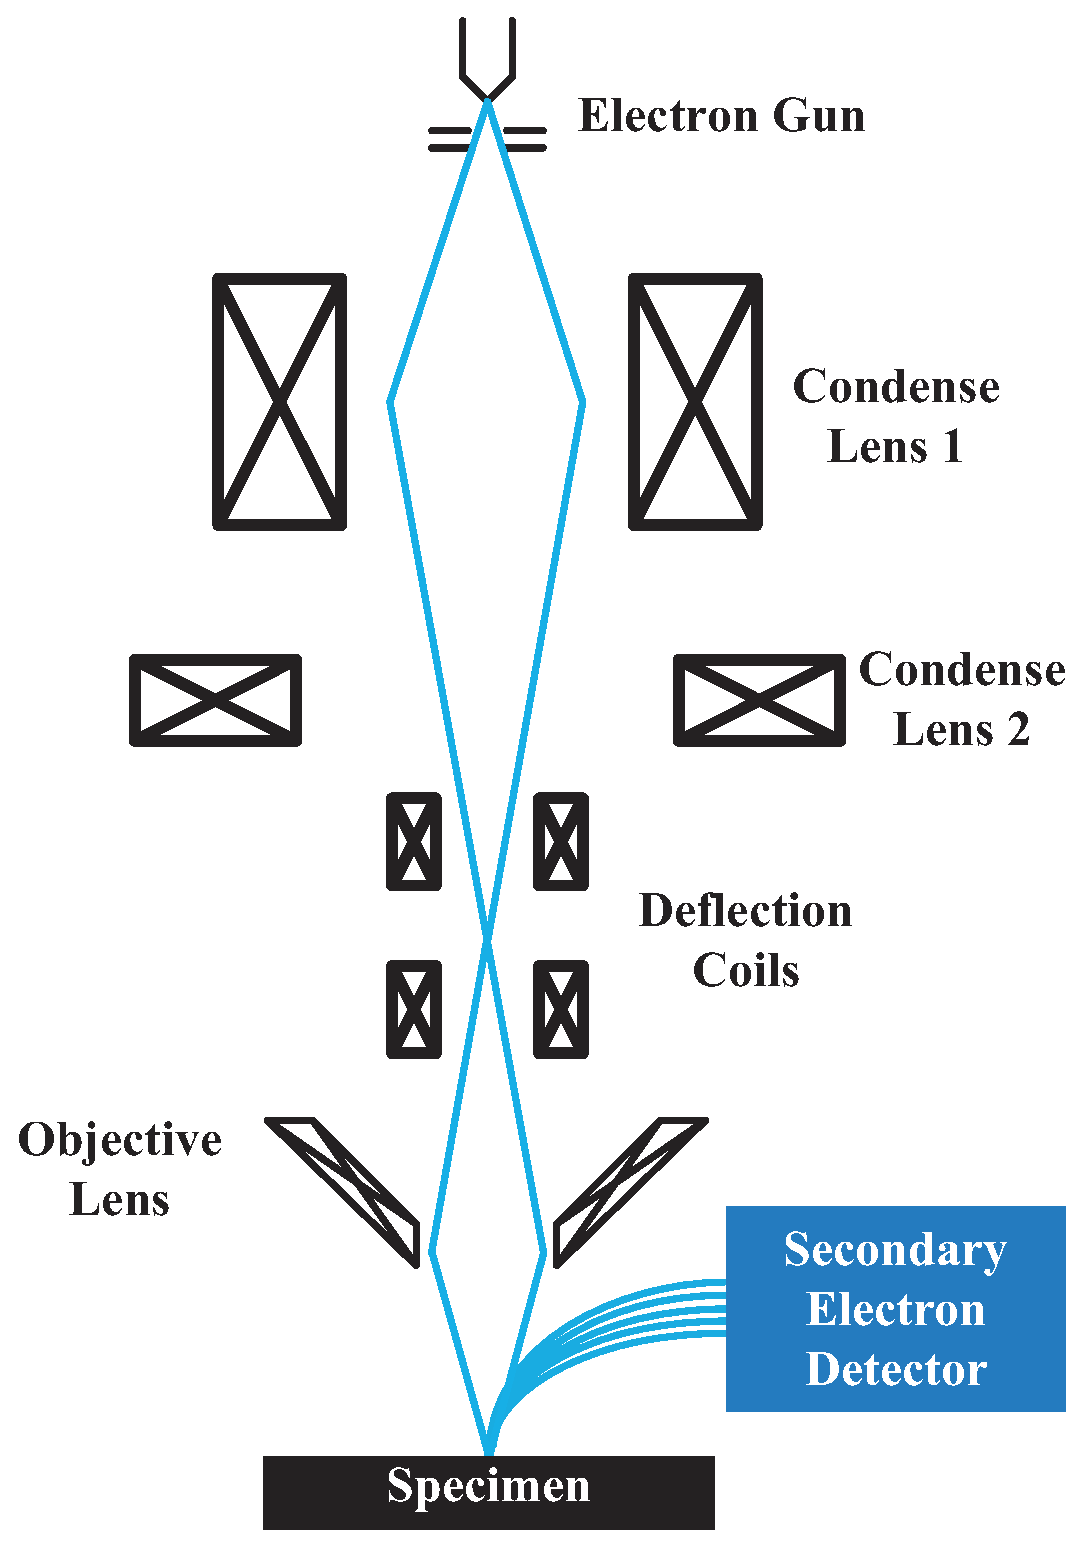
\includegraphics[scale=0.5]{EXP/SEM.eps}
\caption{\label{fig:sem1}Basic construction of a scanning electron microscopy.}
\end{figure}


The JSM-6500F utilizes a Schottky type field-emission (T-FE) gun for the electron source. The T-FE gun can constantly supply the surface of the cathode with zirconium oxide by heating the surface of cathode to 1800 K. For this reason, it can easily obtain stable and high probe current (range from several pA to 100 nA) compared with the traditional thermal emission electron gun and cold field-emission gun.

The magnetic condenser and objective lens system act to control the diameter of the beam as well as to focus the beam on the specimen due to a rotationally-symmetric magnetic field is formed when we pass a direct electric current through a coilwound electric wire in the magnetic lens. A pair of deflector coils, which between the condenser and objective lens, controlled by the scan generator, which are responsible for rastering that focused beam across the specimen surface. The size of the rastering pattern is under magnification control. The beam is rastered from left to right and top to bottom. There is a one-to-one correspondence between the rastering pattern on the specimen and the rastering pattern used to produce the image on the monitor. The resolution we choose to image at will obviously affect the number of pixels per row as well as the number of rows that constitute the scanned area.

The signal is generated from the specimen, and collected by the detector and subsequently processed to generate the image. That processing takes the intensity of the signal coming from a pixel on the specimen and converts it to a grayscale value of the corresponding monitor pixel. The monitor image is a two dimensional rastered pattern of grayscale values.

With the beam focused on the specimen surface, all we need to do to change magnification is to change the size of the rastered area on the specimen. The size of the monitor raster pattern is constant. Magnification will increase if we reduce the size of the area scanned on the specimen.

%\bibliographystyle{unsrt}
%\bibliography{thesisbib}
%\input{main}
%\input{conclusions}

%chapter cite  == \include

%\chapter{Get started with \LaTeX\ }
\label{c:GetStarted}
Three common font styles in this text: 
\begin{itemize}
    \item \textbf{Item1}: \textit{Italic中文123}     
    \item \textbf{Item2}: \textbf{Bold中文123}
    \item \textbf{Item3}: \textsl{slant中文123}
\end{itemize}

About the advance latex grammer see the next section \ref{s:AdvancedFeatures}.


\section{\LaTeX\ Adavanced Features}
\label{s:AdvancedFeatures}
The following features would be introduced in the coming subsections:
\begin{itemize}
    \item SubSection \ref{ss:Fig.}: \hyperref[ss:Fig.]{\textbf{Fig.}}
    \item SubSection \ref{ss:VerbUsage}: \hyperref[ss:VerbUsage]{\textbf{Verb}}
    \item SubSection \ref{ss:VerbUsage}: \hyperref[ss:VerbUsage]{\textbf{Verb}}
    \item SubSection \ref{ss:Enumeration}: \hyperref[ss:Enumeration]{\textbf{Enumeration}}
    \item SubSection \ref{ss:Table}: \hyperref[ss:Table]{\textbf{Table}}
    \item SubSection \ref{ss:CodeDisplay}: \hyperref[ss:CodeDisplay]{\textbf{Code Display}}
    \item SubSection \ref{ss:Math}: \hyperref[ss:Math]{\textbf{Math}}
    \item SubSection \ref{ss:Algorithms}: \hyperref[ss:Algorithms]{\textbf{Algorithms}}
\end{itemize}

%==========================================================================================
\subsection{Fig.}
\label{ss:Fig.}
\begin{figure}[htpb!]
  \centering
    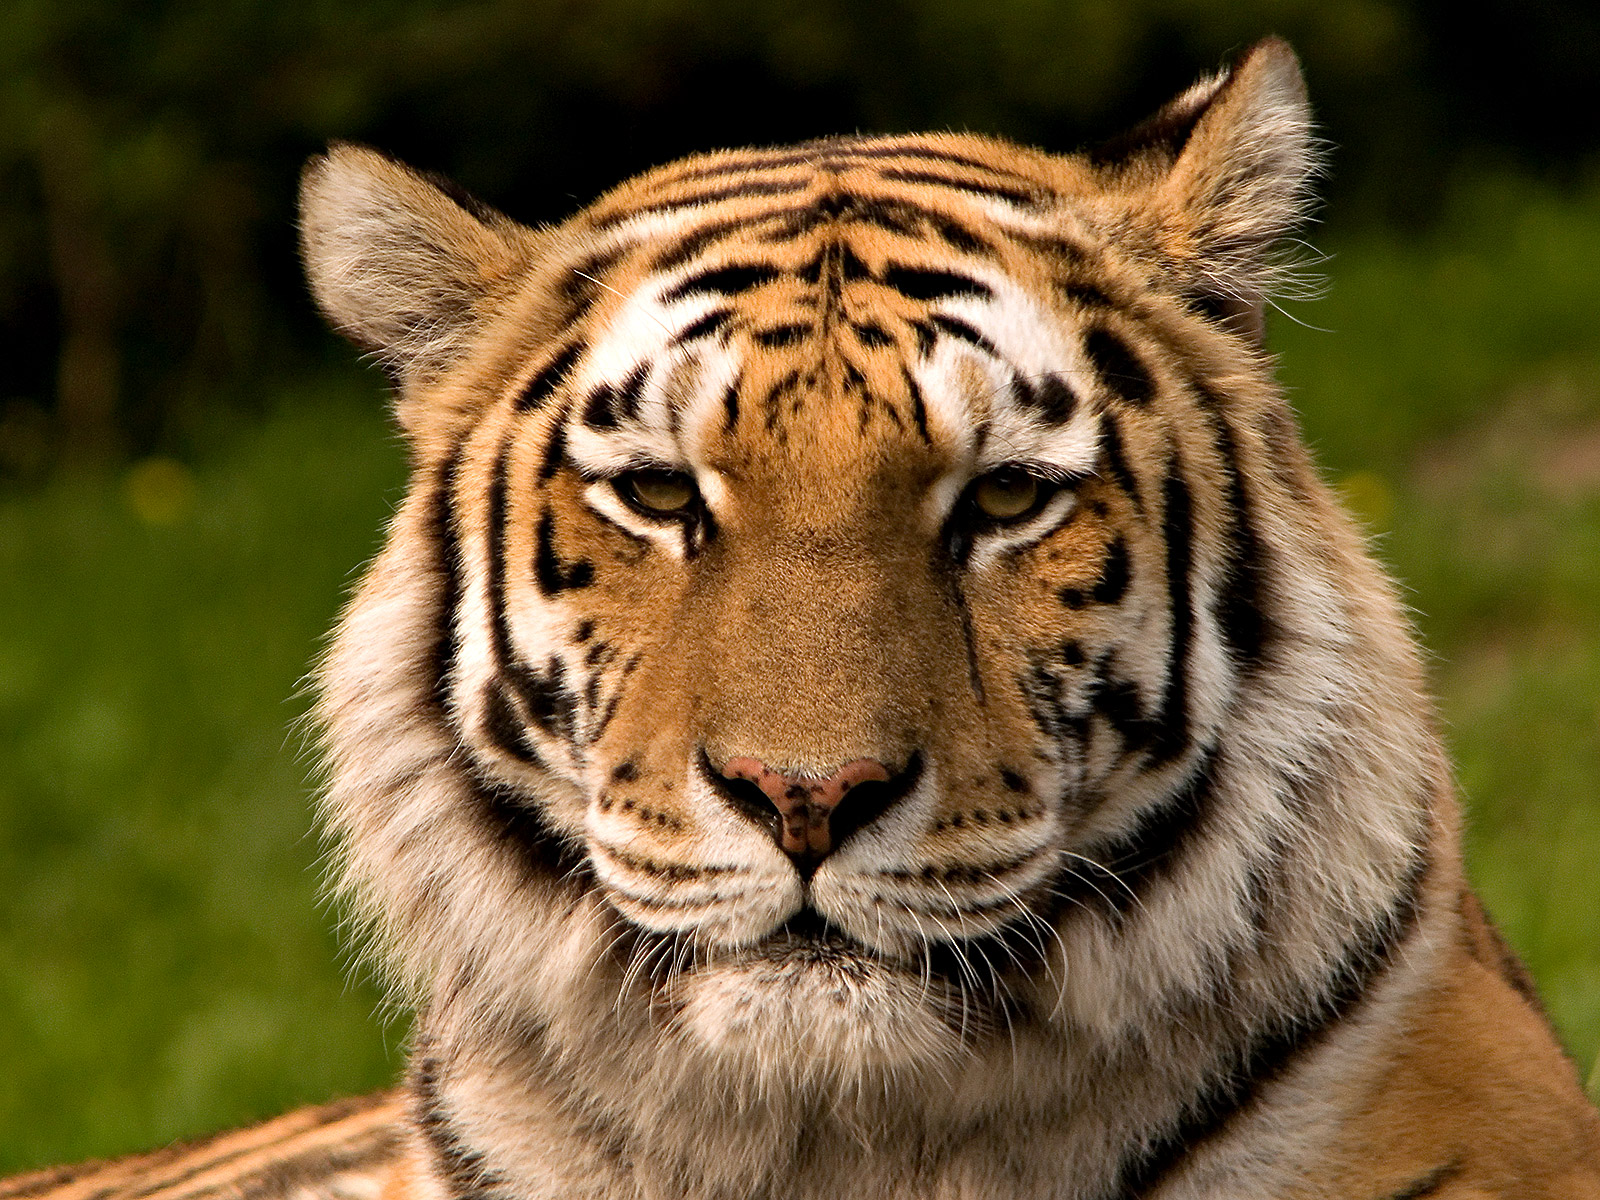
\includegraphics[width=0.5\textwidth]{fig/tiger.jpeg}
    \caption{\label{fig:tiger}A picture of a tiger.}
\end{figure}

Fig.~\ref{fig:tiger} is a picture of a tiger.


%==========================================================================================
\subsection{Table}
\label{ss:Table}

\href{http://en.wikibooks.org/wiki/LaTeX/Tables}{Table examples on WIKIBOOKS}.

\begin{table}[htpb]\begin{center}
\caption{Table Example 1}
\begin{tabularx}{8cm}{llX}
\hline
Start & End  & Character Block Name \\
\hline
3400  & 4DB5 & CJK Unified Ideographs Extension A \\
4E00  & 9FFF & CJK Unified Ideographs \\
\hline
\end{tabularx}
 \end{center}\end{table}

\begin{table}[htpb]\begin{center}
\caption{Table Example 2}
\begin{tabular}{llr}
\hline
\multicolumn{2}{c}{Item} \\
\cline{1-2}
Animal & Description & Price (\$) \\
\hline
Gnat  & per gram & 13.65 \\
      & each     &  0.01 \\
Gnu   & stuffed  & 92.50 \\
Emu   & stuffed  & 33.33 \\
Armadillo & frozen & 8.99 \\
\hline
\end{tabular}
 \end{center}\end{table}
 
 \begin{table}[htpb]\begin{center}
	\label{t:prefix-table}
	\caption{Table Example 3}
	\renewcommand{\arraystretch}{1.0}
	\begin{tabularx}{300pt}{|c|X| }
		\hline
		\multirow{1}{*}{\textbf{Allocation}} &
		Allocation, Element, Type, Script 
		\\ \hline\hline
		%------------------------------
		\multirow{6}{*}{\textbf{Data Types}} &
        Byte2, Byte3, and Byte4\\ &
        Float2, Float3, Float4\\ &
        Int2, Int3, Int4\\ &
        Long2, Long3, Long4\\ &
        Matrix2f, Matrix3f, Matrix4f\\ &
        Short2, Short3, Short4
        \\ \hline\hline
		%------------------------------
		\multirow{4}{*}{\textbf{Graphics}} &
		Mesh\\&
		ProgramFragment, ProgramRaster\\&
		ProgramStore, ProgramVertex\\&
		RSSurfaceView
		\\ \hline
		%------------------------------
	\end{tabularx}
\end{center}\end{table}

\begin{table}[htpb]\begin{center}
\caption{Table Example 4}
\begin{tabular}{|l|l|l|}
\hline
\multicolumn{3}{|c|}{Team sheet} \\
\hline
Goalkeeper & GK & Paul Robinson \\ \hline
\multirow{4}{*}{Defenders} & LB & Lucus Radebe \\
 & DC & Michael Duberry \\
 & DC & Dominic Matteo \\
 & RB & Didier Domi \\ \hline
\multirow{3}{*}{Midfielders} & MC & David Batty \\
 & MC & Eirik Bakke \\
 & MC & Jody Morris \\ \hline
Forward & FW & Jamie McMaster \\ \hline
\multirow{2}{*}{Strikers} & ST & Alan Smith \\
 & ST & Mark Viduka \\
\hline
\end{tabular}
 \end{center}\end{table}
 
 \begin{table}[htpb]\begin{center}
\caption{Table Example 5}
 \begin{tabular}{l*{6}{c}r}
Team              & P & W & D & L & F  & A & Pts \\
\hline
Manchester United & 6 & 4 & 0 & 2 & 10 & 5 & 12  \\
Celtic            & 6 & 3 & 0 & 3 &  8 & 9 &  9  \\
Benfica           & 6 & 2 & 1 & 3 &  7 & 8 &  7  \\
FC Copenhagen     & 6 & 2 & 1 & 2 &  5 & 8 &  7  \\
\end{tabular}
 \end{center}\end{table}

%==========================================================================================
\subsection{Verb}
\label{ss:VerbUsage}
Let's take a overview on how to type special characters:\\
\verb|<FRAMEWORKS_BASE>/graphics/java/android/renderscript|\\\footnote{Path of <APP\_intermediates>: <ANDROID\_ROOT>/out/target/common/obj/APPS/APPNAME\_intermediates/}
You could also go back to the beginning of the chapter by the \hyperref[c:GetStarted]{\textbf{hyperref}}.

%==========================================================================================
\subsection{Enumeration}
\label{ss:Enumeration}
\begin{enumerate}
\item Enumerated Item1
\item Enumerated Item2
\item Enumerated Item3
\end{enumerate}

%==========================================================================================
\subsection{Code Display}
\label{ss:CodeDisplay}

\lstset{
	language=C++,
	stringstyle=\rmfamily,
	commentstyle=\itshape\color[rgb]{0.133,0.545,0.133},
	showstringspaces=false,
	basicstyle=\ttfamily\scriptsize,
	numberstyle=\tiny,
	numbers=left,
	stepnumber=1,
	numbersep=10pt,
	tabsize=2,
	breaklines=true,
	prebreak = \raisebox{0ex}[0ex][0ex]{\ensuremath{\hookleftarrow}},
	breakatwhitespace=false,
  	columns=fixed,
  	upquote=true,
  	extendedchars=true,
	xleftmargin=2em,
	xrightmargin=.5em,
	escapeinside={(*@}{@*)},
    mathescape=false,
}
Here is a "Hello, DanDing." example:
\begin{lstlisting}[style=nonumbers] 
void main(int argc, char **argv)
{
    printf("   ˊ_> ˋ  ");
}
\end{lstlisting}


Another example with line numbers:
\begin{lstlisting}
void main(int argc, char **argv)
{
    printf("   ˊ_> ˋ  ");
}
\end{lstlisting}

Matlab example:

\definecolor{dkgreen}{rgb}{0,0.6,0}
\definecolor{gray}{rgb}{0.5,0.5,0.5}
\lstset{language=Matlab,
   keywords={break,case,catch,continue,else,elseif,end,for,function,
      global,if,otherwise,persistent,return,switch,try,while},
   basicstyle=\ttfamily,
   keywordstyle=\color{blue},
   commentstyle=\color{red},
   stringstyle=\color{dkgreen},
   numbers=left,
   numberstyle=\tiny\color{gray},
   stepnumber=1,
   numbersep=10pt,
   backgroundcolor=\color{white},
   tabsize=4,
   showspaces=false,
   showstringspaces=false}

\begin{lstlisting}
function y = demo(x) % This is a comment.
   str = 'hello there';
   y = x + 1;
end
\end{lstlisting}

%==========================================================================================
\subsection{Math}
\label{ss:Math}
\begin{itemize}
    \item Inline mode:\\
The solution to $\sqrt{x} = 5$ is $x=25$.
    \item Display mode:\\
The solution to \[\sqrt{x} = 5\] is \[x=25.\]
    \item Numbered mode:
\begin{equation}
2+2=4
\end{equation}
    \item Non-numbered:
\begin{equation*}
2+2=4
\end{equation*}
    \item Aligning:
\begin{align*}
2x^2 + 3(x-1)(x-2) & = 2x^2 + 3(x^2-3x+2)\\
&= 2x^2 + 3x^2 - 9x + 6\\
&= 5x^2 - 9x + 6
\end{align*}
     \item Fractions:
\[
 \frac{n!}{k!(n-k)!} = \binom{n}{k}
\]
    \item Matrix:
\[
 A_{m,n} =
 \begin{pmatrix}
  a_{1,1} & a_{1,2} & \cdots & a_{1,n} \\
  a_{2,1} & a_{2,2} & \cdots & a_{2,n} \\
  \vdots  & \vdots  & \ddots & \vdots  \\
  a_{m,1} & a_{m,2} & \cdots & a_{m,n}
 \end{pmatrix}
\]
\end{itemize}
\href{http://en.wikibooks.org/wiki/LaTeX/Mathematics}{More examples on WIKIBOOKS}.


%==========================================================================================
\subsection{Algorithms}
\label{ss:Algorithms}
%\begin{algorithm}[h]                      % enter the algorithm environment
%\caption{Calculate $y = x^n$}          % give the algorithm a caption
%\label{alg1}                           % and a label for \ref{} commands later in the document
%\begin{algorithmic}                    % enter the algorithmic environment
    %\Require $n \geq 0 \vee x \neq 0$
    %\Ensure $y = x^n$
    %\State $y \Leftarrow 1$
    %\If{$n < 0$}
        %\State $X \Leftarrow 1 / x$
        %\State $N \Leftarrow -n$
    %\Else
        %\State $X \Leftarrow x$
        %\State $N \Leftarrow n$
    %\EndIf
    %\While{$N \neq 0$}
        %\If{$N$ is even}
            %\State $X \Leftarrow X \times X$
            %\State $N \Leftarrow N / 2$
        %\Else[$N$ is odd]
            %\State $y \Leftarrow y \times X$
            %\State $N \Leftarrow N - 1$
        %\EndIf
    %\EndWhile
%\end{algorithmic}
%\end{algorithm}
\href{http://en.wikibooks.org/wiki/LaTeX/Algorithms_and_Pseudocode}{More examples on WIKIBOOKS}.


%\chapter{Introduction}
\framebox{REVIEW1}
\section{Motivation}
%Robot => speech => MIDI (history)
From the machnical music performing antomata, to the Japanese virtual signer Hatune Miku, there had been many attempts to create autoated system that performs music. However, many of these system can only perform predefined expression, which is not very satisfying. State-of-the-art text-to-speech system can already generate fluid and natural speech, but computer performance still can't perform very expressivly.

Therefore, many researcher have devoted many effort to develop systems that can automatically or semi-automatically perform music expressively. There is even a biannual contest called Music Performance Rendering Contest (RenCon)\cite{RenCon} that puts all performance system to into competition. Their roadmap suggest that they wish to win the Chopin International Piano Contest by a computer perforer. We will review previous works, including many which won the RenCon prizes, in Chapter \ref{chap:prev}.
%Computer generated music, such as synthsized MIDI, are often considered robotic and unexpressive. But we have already witnessed the fluid and lively sound generated by state-of-the-art text-to-speech systems. This inspired us to develop a system that can read a music score and play it in an expressive, humanly way. Such system can be used for audiolizing score notation editing software, creating interactive media content, and generating royality-free music. 

%Established pianists always has his/her own distinctive style. Such sytle distinguised himself/herself from all the other pianists. If the expressive performance system can learn the style of a performer, it might be able to provide musicological insight of performance styles. Furthermore, we can even make a mastero who is no longer with us play music he/she never played in his/her lifetime.

There are many applications for a computer expressive performance system, many commercial music typesetting software like Finale and Sibelius already have expressive playback features built-in. On the commercial side, such system can provide personalized music listening experience. For the music production industry, it saved a lot of cost on hiring musicians or licensing. Such system can also opens up new opportunity in music making, such as human-machine co-performance, or interactive multimedia installation. In academia, researchers can use this technology to model the performing style of musicians, or restore historical music archive.

\framebox{TODO:Discuss Mazolla's theroy of expressive performance}

%\begin{figure}[tp]
%   \begin{center}
%      %TODO:Fig.: expressive performance concept
%      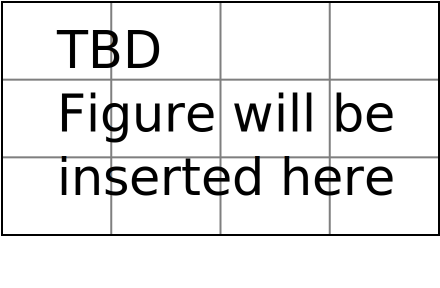
\includegraphics[width=\textwidth]{fig/TBDFigure}
%
%   \end{center}
%   \caption{From Composer to Performance}
%   \label{fig:concept}
%\end{figure}
%Application: musicology study, typesetting tool, play score archive, play computer-generated music, accompaniment



\section{Goal and Contribution}
\framebox{TODO:brief guide to previous works}
There are many different goals for computer expressive performance, which will be discussed in Chapter \ref{chap:prev}. In this research the ultimate goal is to be able to play any music in any expressive style specified. But due to the technical and time constrain, we need to set a more practical goal for our research. We wish to build a computer expressive performance system based on an offline supervised learning algorithm. The system will be able to learn any play monophonic musical phrases. The expressiveness will be at phrase level, structural or timbre related expression are not the primary concern. The performance style will be controlled by the learning material, which is traditional music notation, with human-annotated phrasing information. If only recordings from a single performer is given, it should learn the particular style of the performer.


The major contribution of this thesis is that we apply structural support vector machine on expressive performance problem. There exist no previous work that uses the discriminative learning power of support vector machine on computer expressive performance question. We also developed methods and tools to generate corpus for expressive performance system based on learning algorithms. 
%\bibliographystyle{unsrt}
%\bibliography{thesisbib}
\section{Chapter Organization}
In Chapter \ref{chap:prev}, we will give an overview of previous works and their varying goals, the works will be grouped by the way they learn performance knowledge, and finally we will discuss some additional specialities such as special instrument model or special user interaction pattern. In Chapter \ref{chap:proposed}, we will first give a brief introduction to the mathematical background of the learning algorithm, SVM-HMM. And then we will provide a top-down explanation to the proposed method. Then in Chapter \ref{chap:corpus}, we will explain how the corpus used for training is designed and implemented. Finally, In Chapter \ref{chap:exp}, we will show several experiment results and discussions. We have also included two appendixes, appendix \ref{chap:sw} presents some software tools used in this research, which may be helpful for other researchers in music and machine learning fields.

%\chapter{Theory of surface plasmon polaritons in metallic nano-structures}
\label{c:thm}
\section{Definition of plasmon}

Plasmon is collective oscillation of conduction electron gas, a quasi-particle resulting from the quantization of plasma oscillations just like phonons are quantizations of mechanical vibrations. The simplest case is the volume plasmon as shown in Figure~\ref{fig:bulk}.
\begin{figure}[htb]
\centering
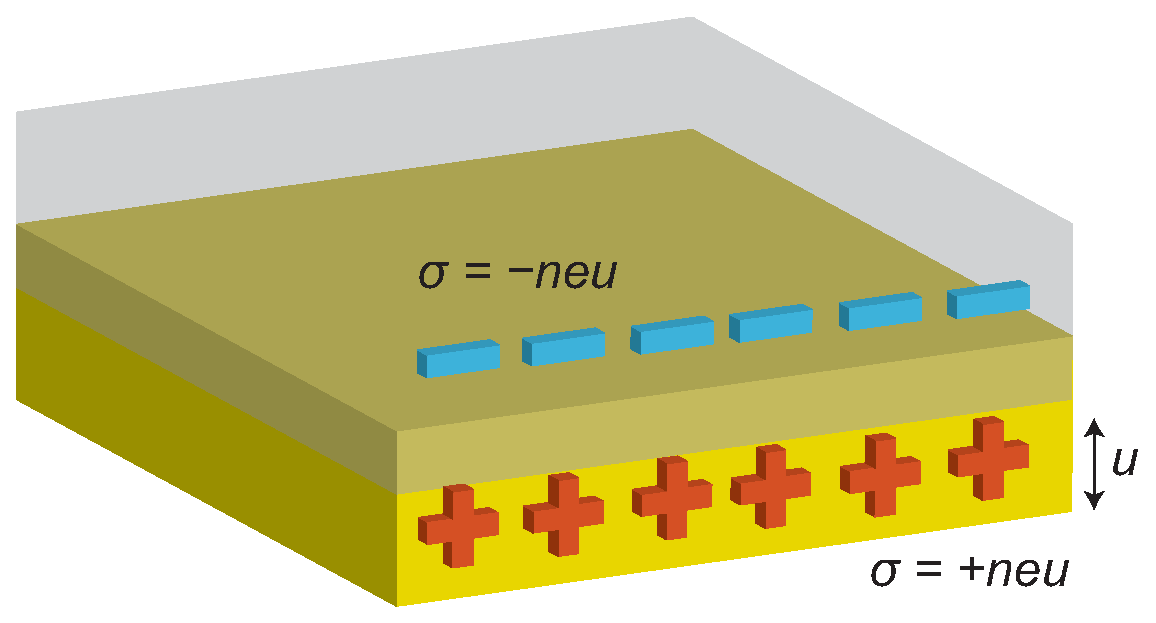
\includegraphics[scale=0.5]{THM/bulk.eps}
\caption{\label{fig:bulk}Longitudinal collective oscillations of the conduction electrons of a metal (Volume plasmons)}
\end{figure}
 We can derive plasma frequency $\omega_p$ from the simple harmonics oscillation model, a collective displacement of the electron cloud by a distance $u$ leads to a surface charge density $\sigma = \pm neu$ at the slab boundaries. This establishes a homogeneous electric field $\mathbf{E} = \frac{neu}{\varepsilon_0}$ inside the slab. Thus, the displaced electrons experience a restoring force, and their movement can be described by the equation of motion $nm\ddot{u} = -ne\mathbf{E}$. Inserting the expression for the electric field, this leads to
 \begin{subequations}
 \begin{align}
 nm\ddot{u} = -\frac{n^2e^2u}{\varepsilon_0} \\
 \ddot{u} + {\omega_p}^{2}u = 0\text{.}
 \end{align}
 \end{subequations}
  The plasma frequency $\omega_p = \sqrt{\frac{ne^2}{\varepsilon_0m}}$ can thus be recognized as the natural frequency of a free oscillation of the electron sea. The quanta of these charge oscillations are called plasmons. Due to the longitudinal nature of the excitation, volume plasmons do not couple to transverse electromagnetic waves, and can only be excited by particle impact. We can derive the dispersion relation of the generalization of volume plasmons, traveling plasma waves, from curl electric field equations (Equations~\ref{eq:curlE})
 \begin{subequations}
 \begin{align}
 \curl{\curl \mathbf{E}} &= -\mu_0 \frac{\partial^2\mathbf{D}}{\partial t^2}\label{eq:curlE}\\
\mathbf{K}( \mathbf{K}\cdot \mathbf{E}-K^{ 2 }\mathbf{E} ) &=-\varepsilon ( \mathbf{K},\omega  ) \frac { { \omega  }^{ 2 } }{ { c }^{ 2 } } \mathbf{E}
 \end{align}
 \end{subequations}  
and plasma model, and a simple equation of motion for an electron of the plasma subjected to an external electric field $\mathbf{E}$
 \begin{equation}
m\ddot{\mathbf{x}} + m\gamma\dot{\mathbf{x}} = -e\mathbf{E}\text{.}
\end{equation}
Assuming a harmonic time dependence $\mathbf{E}( t )=\mathbf{E}_0\mathrm{e}^{-i\omega t}$ of the driving field, a particular solution of this equation describing the oscillation of the electron is $\mathbf{x} ( t ) = \mathbf{x}_0 \mathrm{e}^{-i\omega t} $. The complex amplitude $\mathbf{x}_0$ incorporates any phase shifts between driving field and response via
\begin{equation}
\mathbf{x} ( t ) = \frac{e}{m( \omega^2 + i\gamma\omega )}\mathbf{E}( t )\text{.}
\end{equation}
The displaced electrons contribute to the macroscopic polarization
\begin{equation}
\mathbf{P}=-\frac{ne^2}{m( \omega^2 + i\gamma\omega )}\mathbf{E}( t )\text{.}
\end{equation}
Inserting $\mathbf{P}$ into dielectric displacement field equation $\mathbf{D} = \varepsilon_0\mathbf{E} + \mathbf{P}$ yields
\begin{equation}
\mathbf{D} = \varepsilon_0(1-\frac{\omega_p^2}{\omega^2 + i\gamma\omega})\mathbf{E}\text{,}
\end{equation}
where $\omega_p^2 = \frac{ne^2}{\varepsilon_0m}$. Therefore, the dielectric function of the free electron gas
\begin{equation}
\varepsilon(\omega) = 1- \frac{\omega_p^2}{\omega^2 + i\gamma\omega}\text{.}\label{eq:dielefu}
\end{equation}
We arrive at the desired result by using equation~\ref{eq:dielefu} and the generic dispersion relation $K^2=\varepsilon(\mathbf{K},\omega)\frac{\omega^2}{c^2}$, the dispersion relation of traveling waves becomes
\begin{equation}
\omega^2 = \omega_p^2 + \mathbf{K}^2c^2\text{.}
\end{equation}
From this relation, we can figure out the oscillation properties in any frequency of external field. Note that this branch can not confine the electromagnetic waves, it would radiate out the energy, so this mode is also called radiative surface plasmon.

\section{Surface plasmon polaritons at interface between dielectric and metal}

Surface plasmon polaritons (SPPs) are eigenmodes of transverse magnetic (TM) waves, which coupling the electromagnetic fields to oscillations of the conductor's electron plasma, propagate at a interface between dielectric and metal, and are confined in perpendicular direction. Providing a flat interface between dielectric and metal half-spaces with dielectric constants $\varepsilon_d$ and $\varepsilon_m$ , respectively, and assuming the interface normal to z direction and the SPPs propagate along the $x$ direction, the SPP wave vector $\beta$ is related to the frequency $\omega$ through the dispersion relation
\begin{equation}
\beta = k_0\sqrt{\frac{\varepsilon_d\varepsilon_m}{\varepsilon_d + \varepsilon_m}}\text{,}\label{eq:sppsdisp}
\end{equation}
where $k_0 = \omega/c$ is the free-space wave vector. We take $\omega$ to be real and allow $\beta$ to be complex.

The optical response of metals is often described by the Drude model for a free-electron gas~\cite{kittel1976introduction},
\begin{equation}
\varepsilon_{Drude}(\omega)=1-\frac{\omega_p^2}{\omega^2+i\Gamma\omega}\text{,}
\end{equation}
in which $\Gamma$ is a damping rate due to electron-electron and electron-phonon scattering.
Figure~\ref{fig:SPPdisp} shows the dispersion curve~\ref{eq:sppsdisp} with Drude metal  in the absence of losses ($\Gamma=0$) for air ($\varepsilon_d = 1$) and fused silica ($\varepsilon_d = 2.25$) interface.
\begin{figure}[htb]
\centering
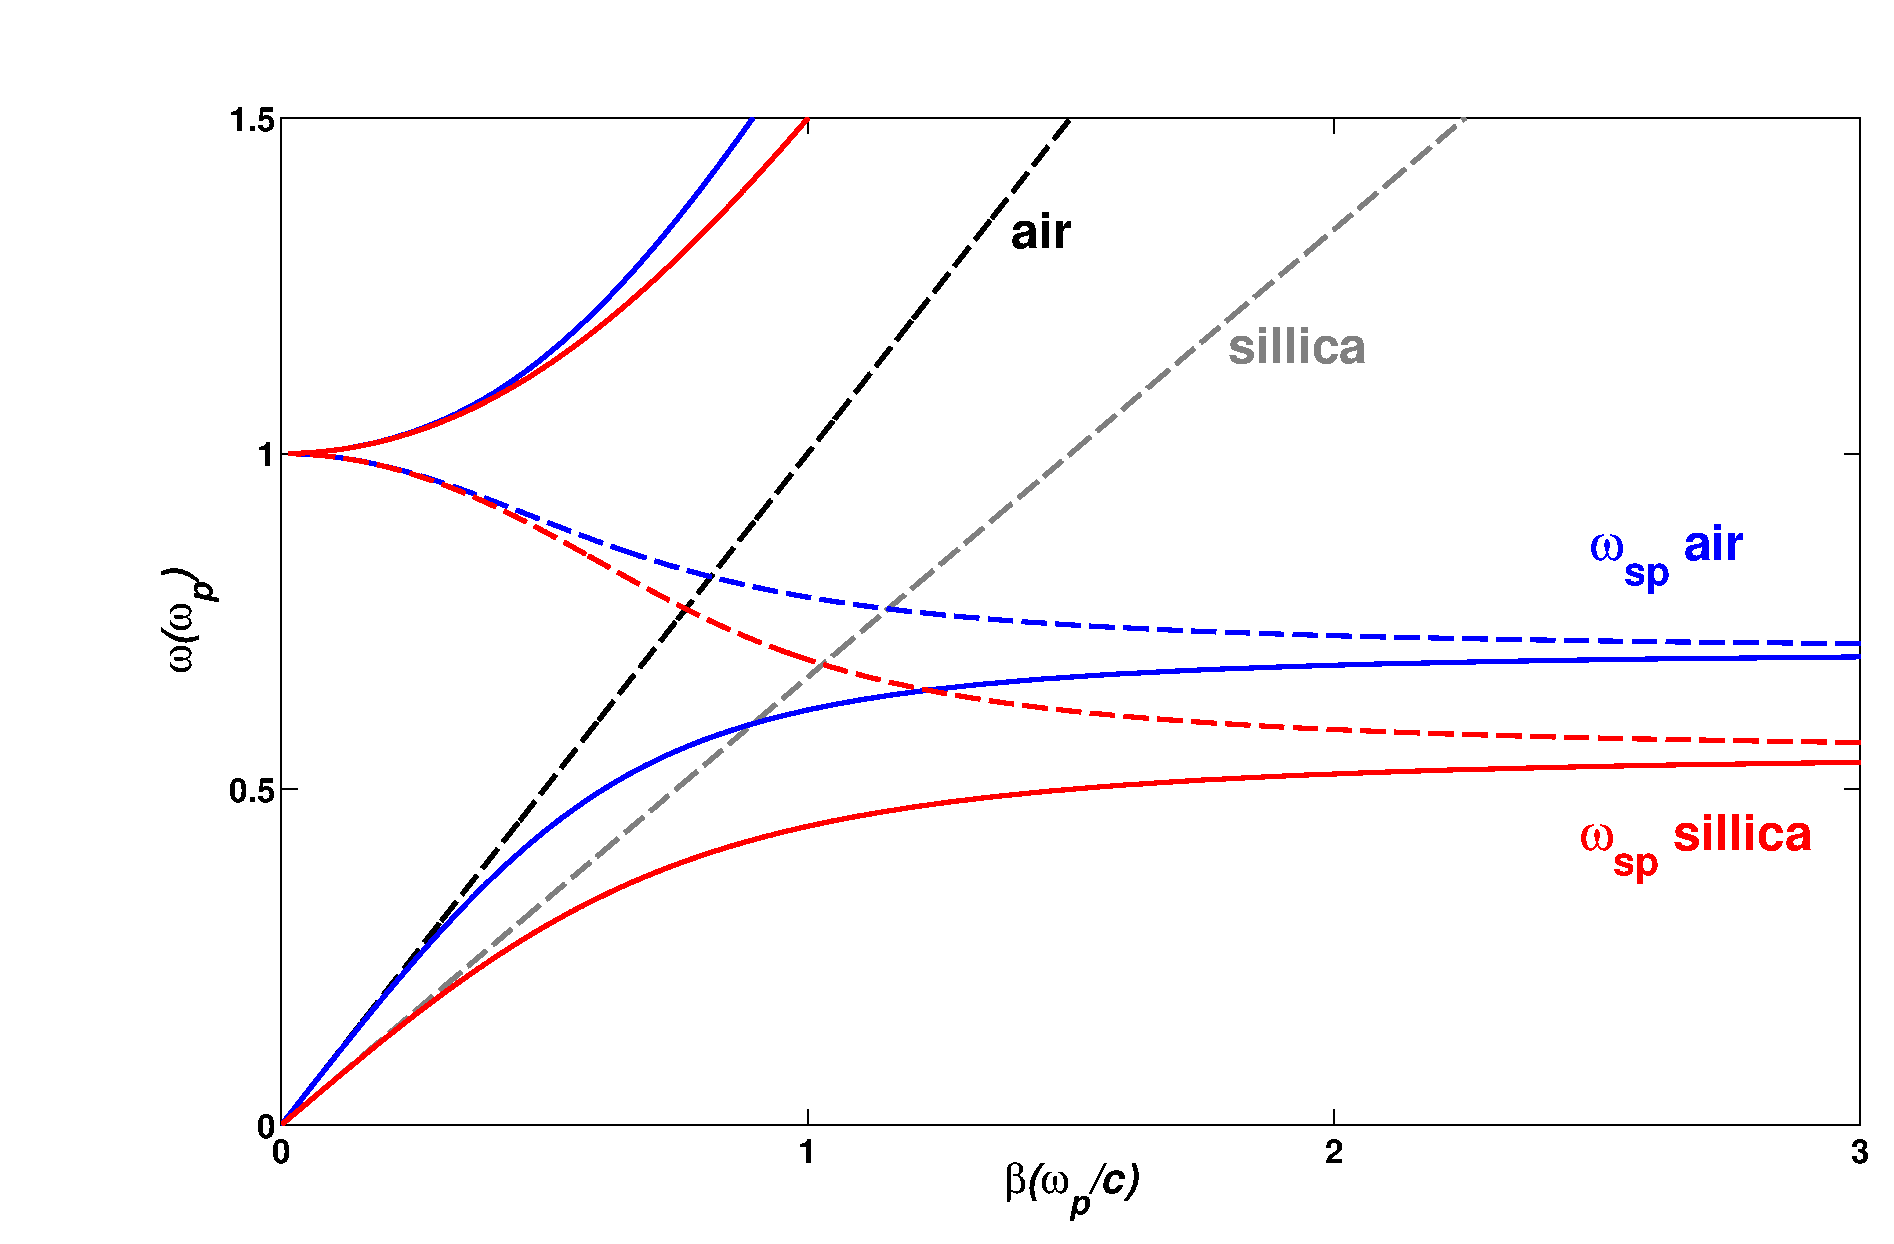
\includegraphics[scale=0.4]{THM/SPPdisp.eps}
\caption{\label{fig:SPPdisp}Dispersion relation of SPPs at the interface between a Drude metal with negligible collision frequency and air (blue curves) and silica (red curves).}
\end{figure}
For small wave vectors SPPs propagation constant $\beta$ is close to $k_0$ at the light line, in the opposite regime of the frequency close to surface plasmon frequency $\omega_p$. It also shows that the SPPs line lying to the right of the respective light lines of air and silica, so that SPPs are directed by light due to phase mismatching. The wave vector mismatch between SPPs and radiation modes needs to be overcome in order to excite or detect SPPs. This can be achieved by multiple methods~\cite{raether1988surface}. In the Otto configuration, light in a prism that is brought in close vicinity to a metal surface can excite SPPs through coupling to the evanescent field. Because light in the prism has a larger wave vector than that in air, it can be phase-matched to the SPPs. In the related Kretschmann-Raether geometry, coupling to SPPs occurs through a metal film that is deposited on a prism. In the grating coupling configuration, metal surface with a shallow grating of grooves or holes with lattice constant $a$. For the simple 1D grating of grooves depicted in Figure~\ref{fig:grating},
\begin{figure}[htb]
\centering
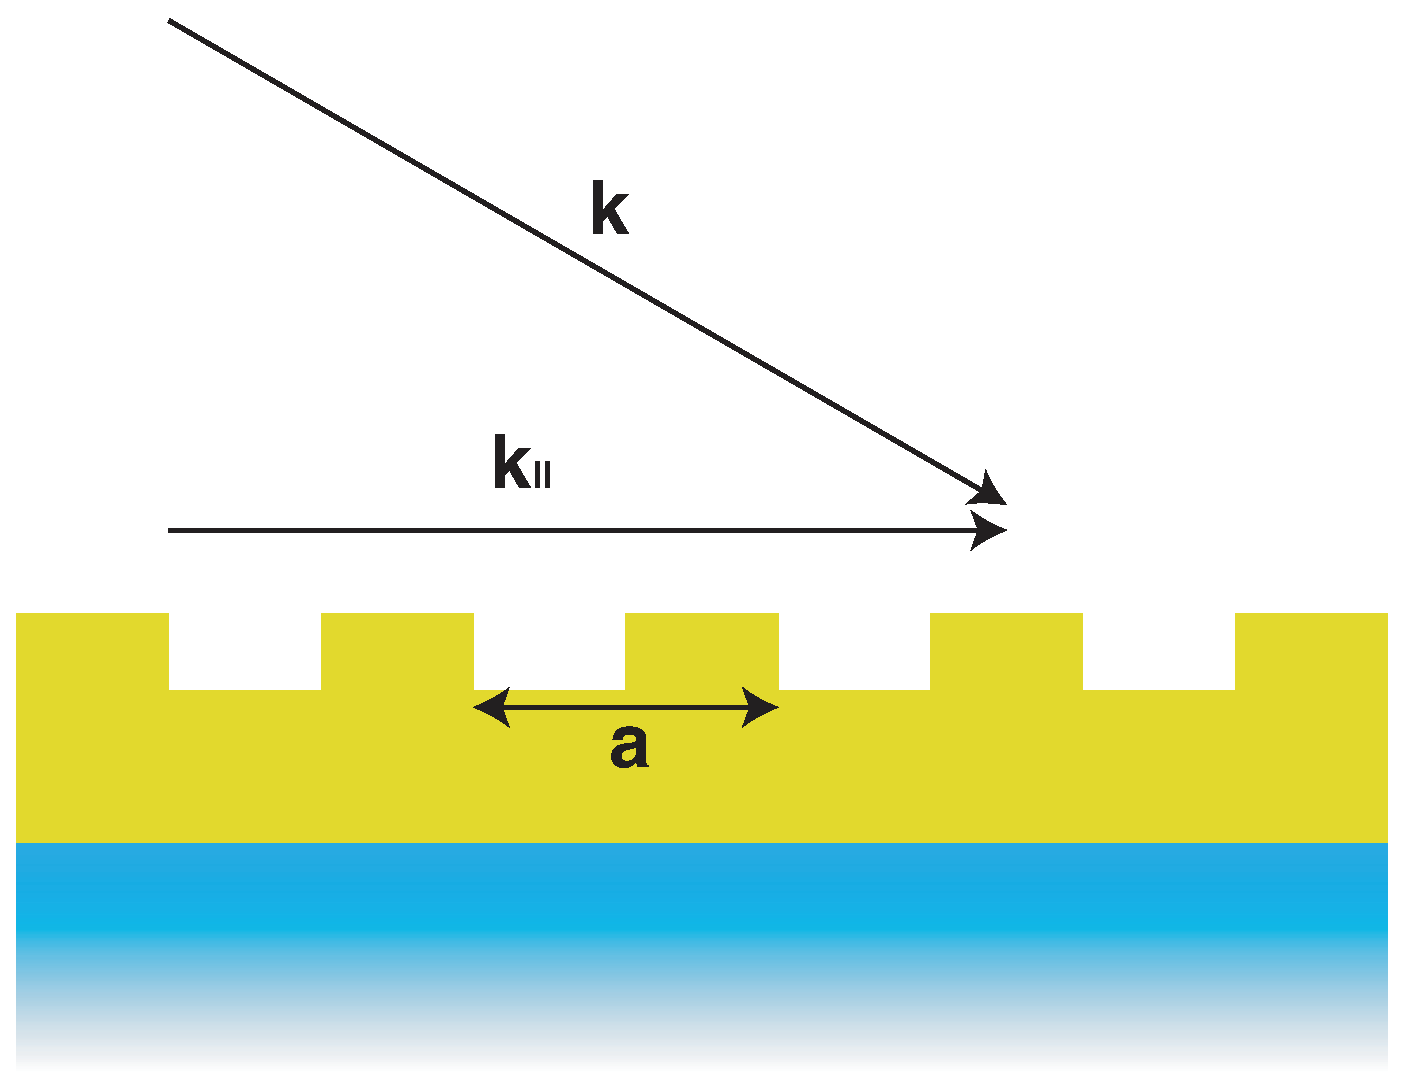
\includegraphics[scale=0.5]{THM/grating.eps}
\caption{\label{fig:grating}Phase-matching of light to SPPs the grating coupling configuration.}
\end{figure}
phase-matching takes place when the condition is fulfilled
\begin{equation}
\beta = k_0 \sin{\theta} \pm \nu g\text{,}
\end{equation}
where $g=\frac{2\pi}{a}$ is the reciprocal vector of the grating, and $\nu=(1,2,3\dots)$.
As with prism coupling, excitation of SPPs is detected as a minimum in the reflected light. The reverse process can also take place, SPPs propagating along a surface modulated with a grating can couple to light and thus radiate. 

%\bibliographystyle{unsrt}
%\bibliography{thesisbib}
%\chapter{Experiment}
\label{c:exp}

\section{Atomic force microscopy}

\begin{figure}[htb]
\centering
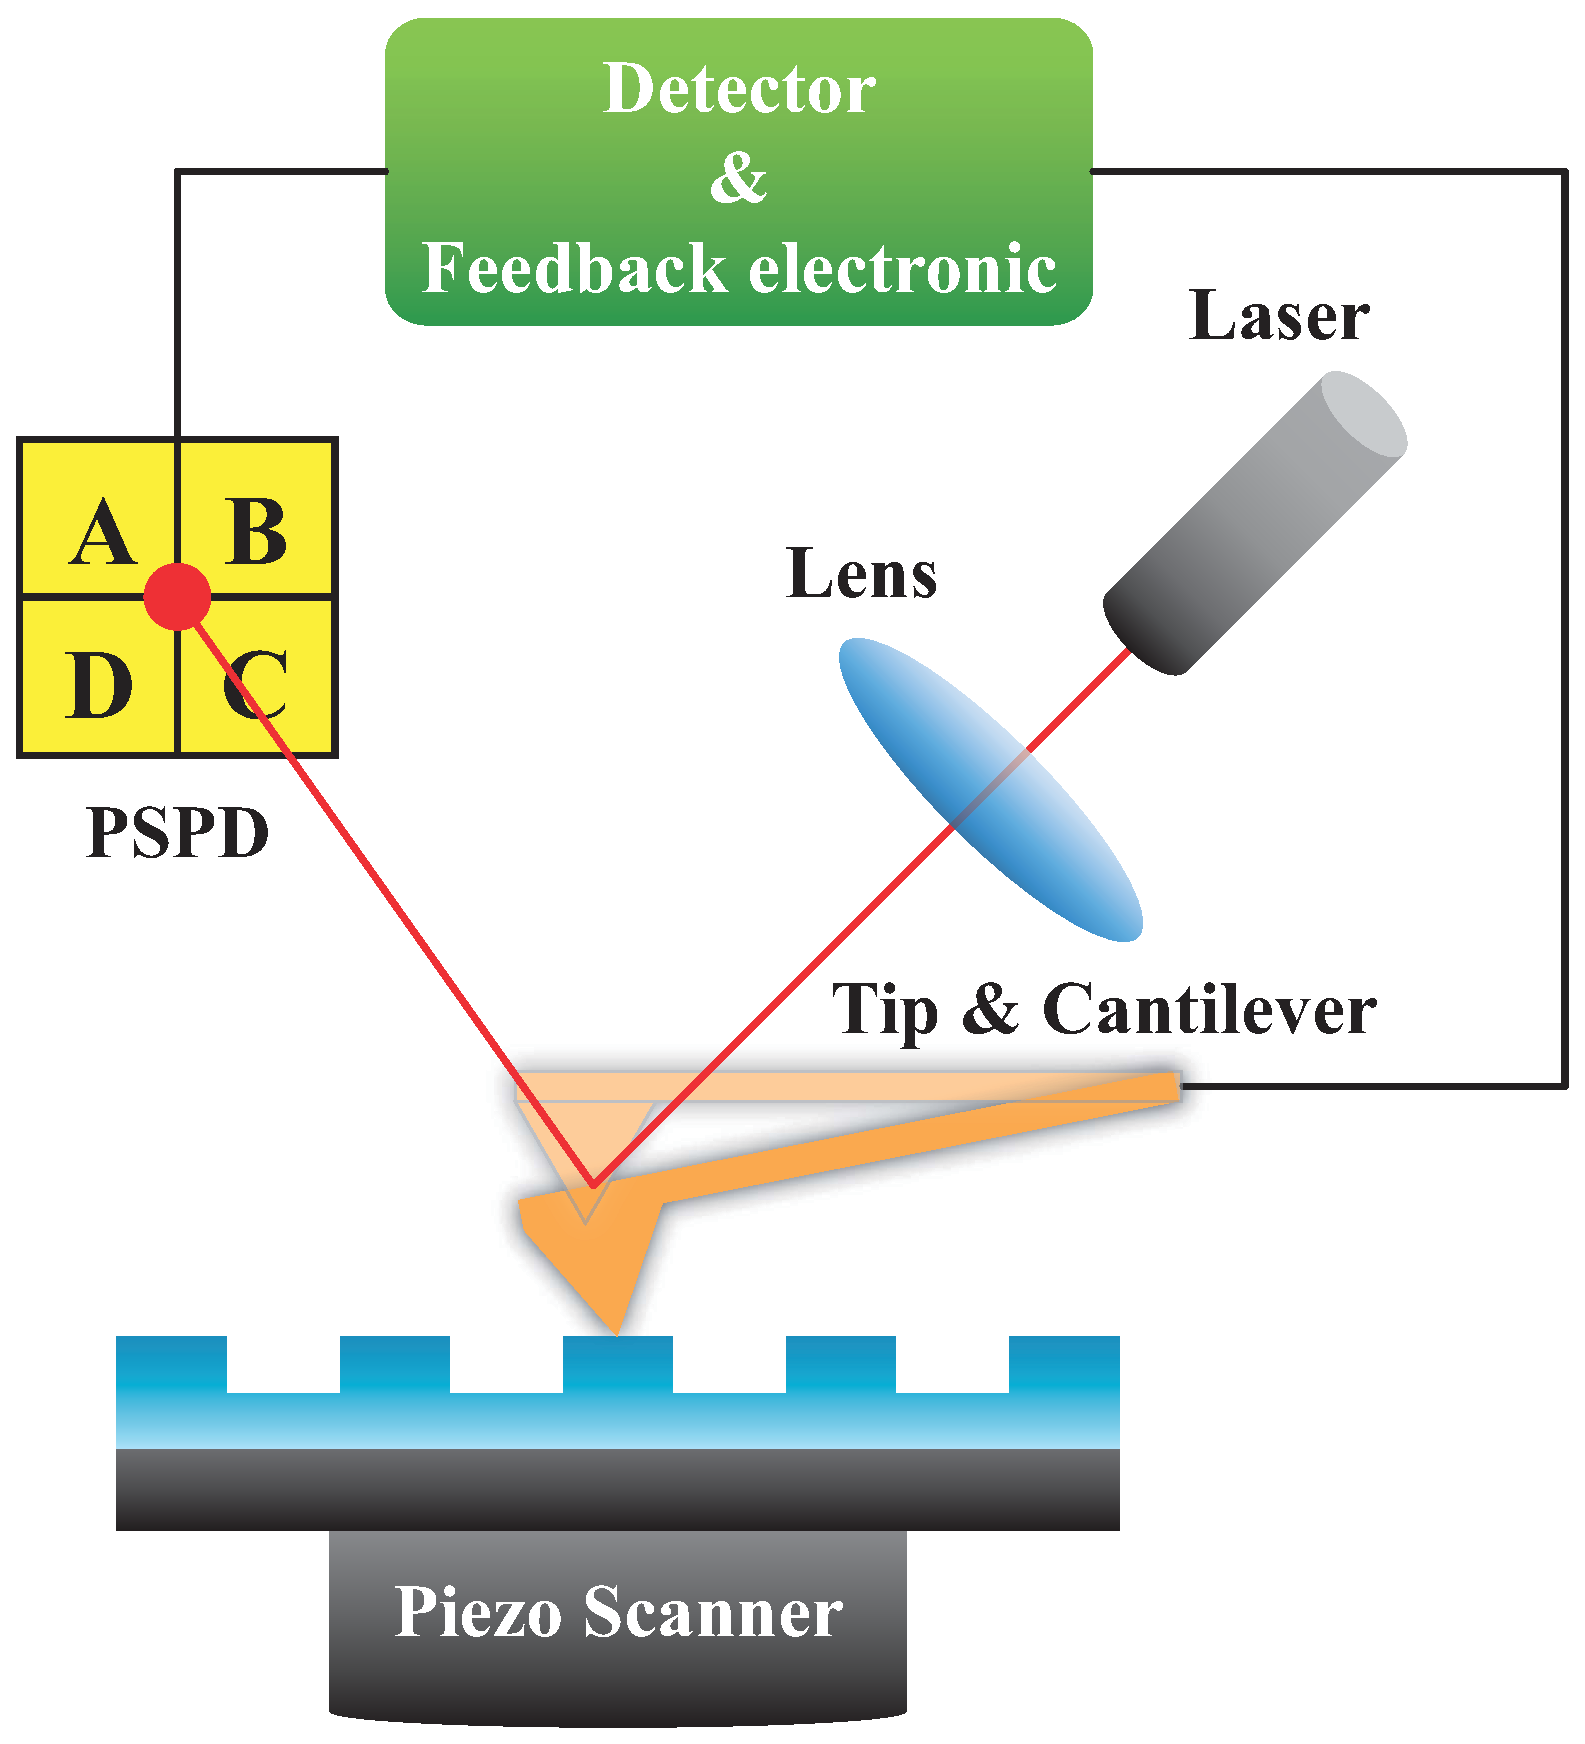
\includegraphics[scale=0.35]{EXP/afm1.eps}
\caption{\label{fig:afm1}Schematic of atomic force microscopy.}
\end{figure}
Atomic force microscope (AFM) is a type of scanning probe microscopes (SPM)~\cite{bennig1988atomic}.  The schematic of AFM is shown in Figure~\ref{fig:afm1}. AFM operates by measuring force between a probe and the specimen surfaces. In general,  the probe is a sharp tip at a cantilever's end. The cantilever can be deflected by atomic forces to sufficiently large amount, then AFM can measure the vertical and lateral deflections of the cantilever by using the optical system. A laser beam is transmitted to cantilever, and the reflected laser beam is detected with a position-sensitive photo detector (PSPD). PSPD is four-sectional that allows measuring not only vertical but lateral bending too(Figure~\ref{fig:afm2}). The output of the PSPD is provided to a computer for processing of the data for providing a topographical image of the surface with atomic resolution, and controlling the height between probe and specimen surfaces by applying voltage on piezoelectric scanner.
\begin{figure}[htb]
\centering
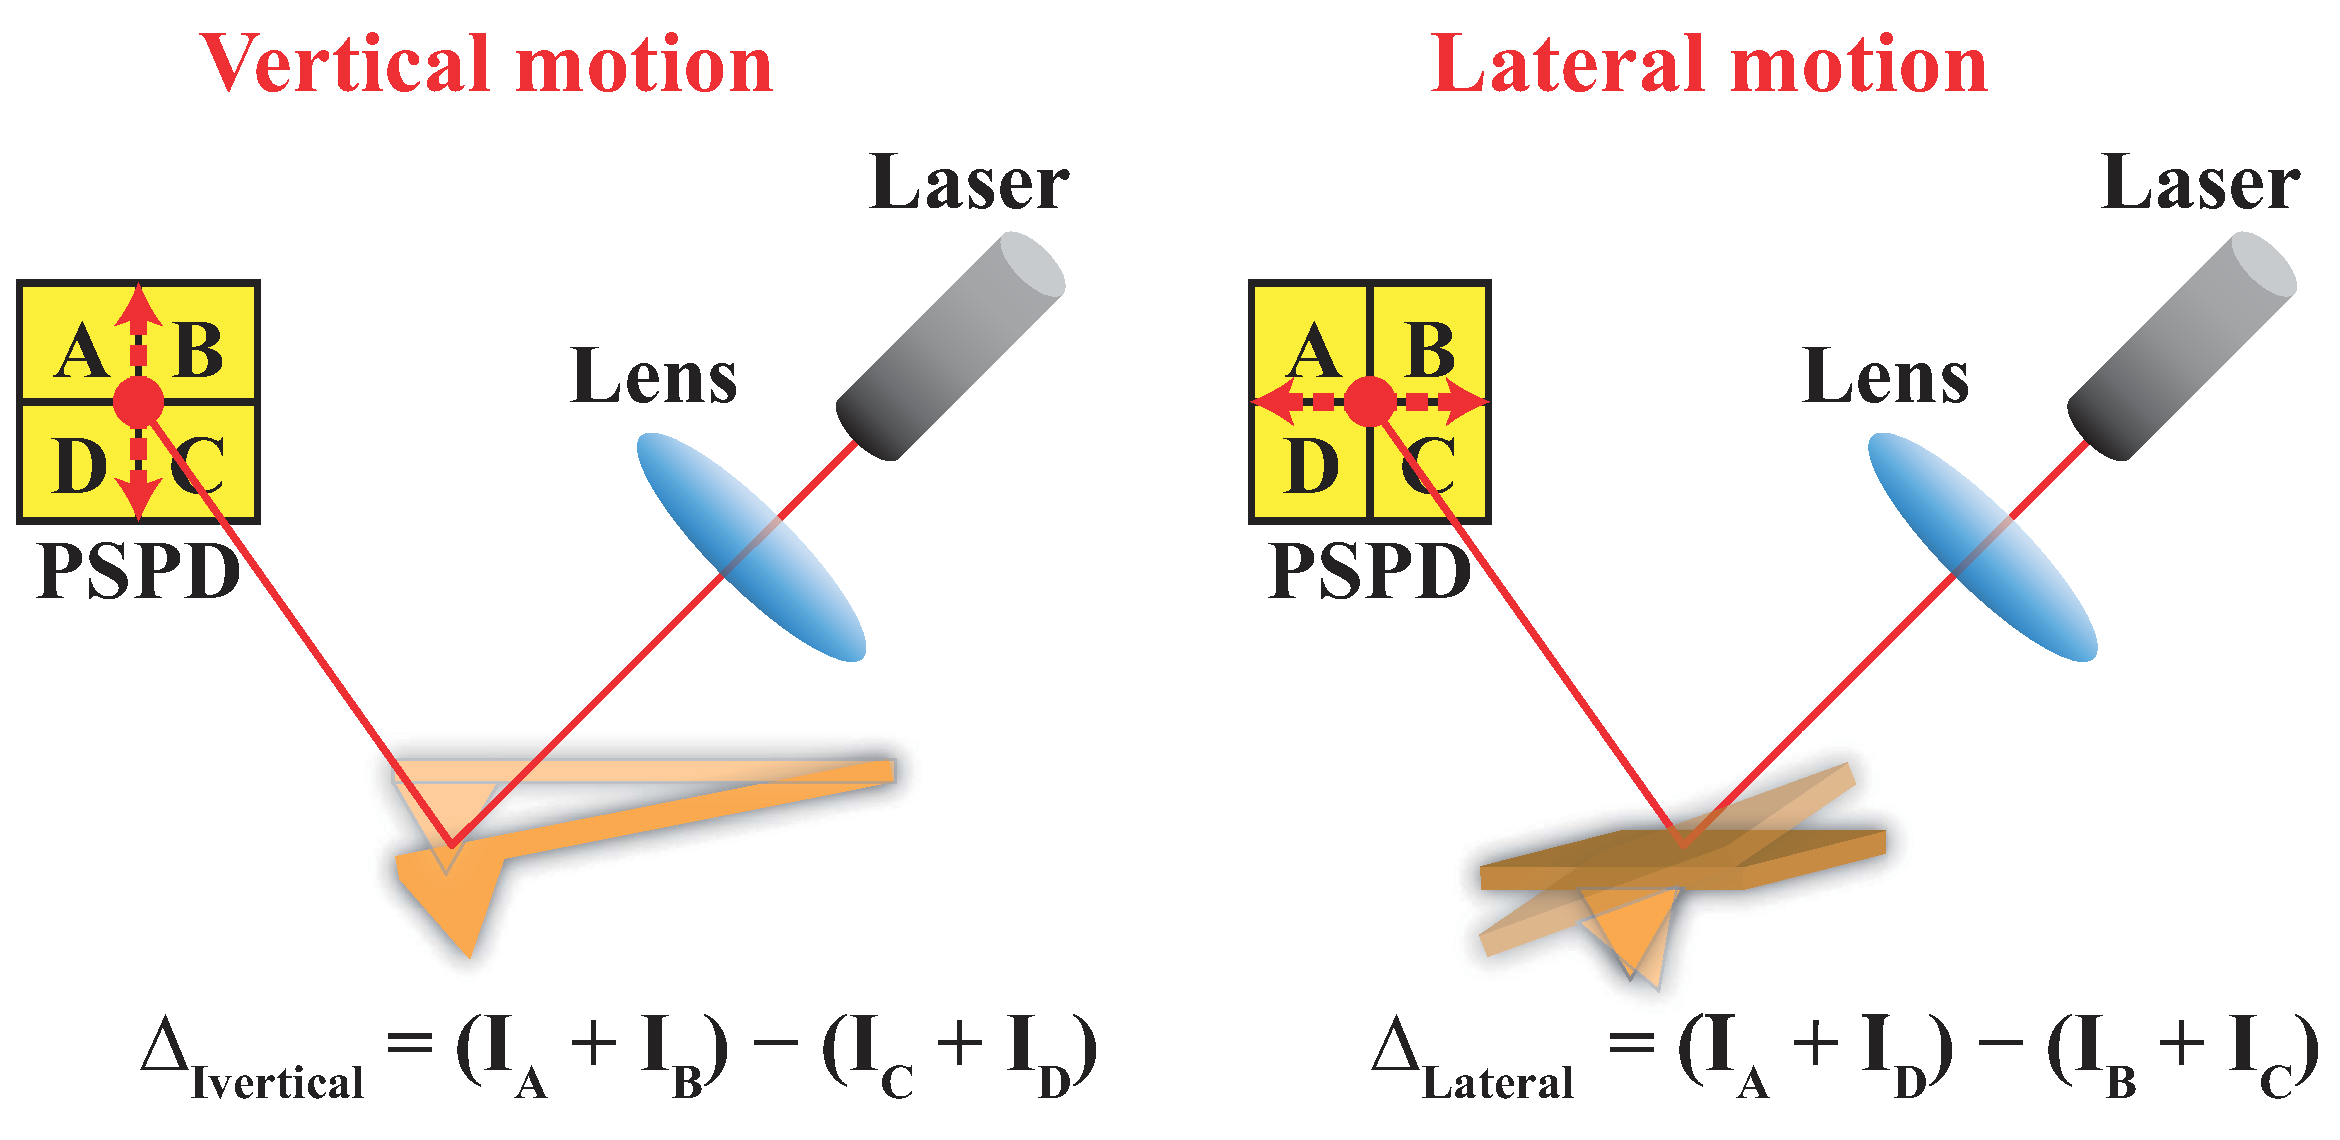
\includegraphics[scale=0.4]{EXP/afm2.eps}
\caption{\label{fig:afm2}Schematic of optical system for cantilever deflections detection.}
\end{figure}

The physical principle of the AFM operation is based on interaction between the probe tip and the specimen surface(Figure~\ref{fig:afm3}). When the cantilever approaches the specimen surface, Van der Waals forces start acting upon it . They are sufficiently far-ranging and are felt at the distance of a few tens of angstroms. Then at the distance of several angstroms repulsive force starts acting. In humid air a water layer is present on the specimen surface. The capillary force arises that holds the tip in contact with the surface and increases the minimum achievable interaction force. Electrostatic interaction between the probe and the sample may appear rather often. This can be both attraction and repulsion. Van der Waals attraction forces, capillary, electrostatic and repulsion forces at the point where the tip touches the sample and forces acting upon the tip from the deformed cantilever compensate each other in equilibrium. Based on the type and degree of this interaction the AFM modes can be broken down into contact and semi-contact(Figure~\ref{fig:afm3} ), which is a transition mode between the contact and non-contact modes.
\begin{figure}[htb]
\centering
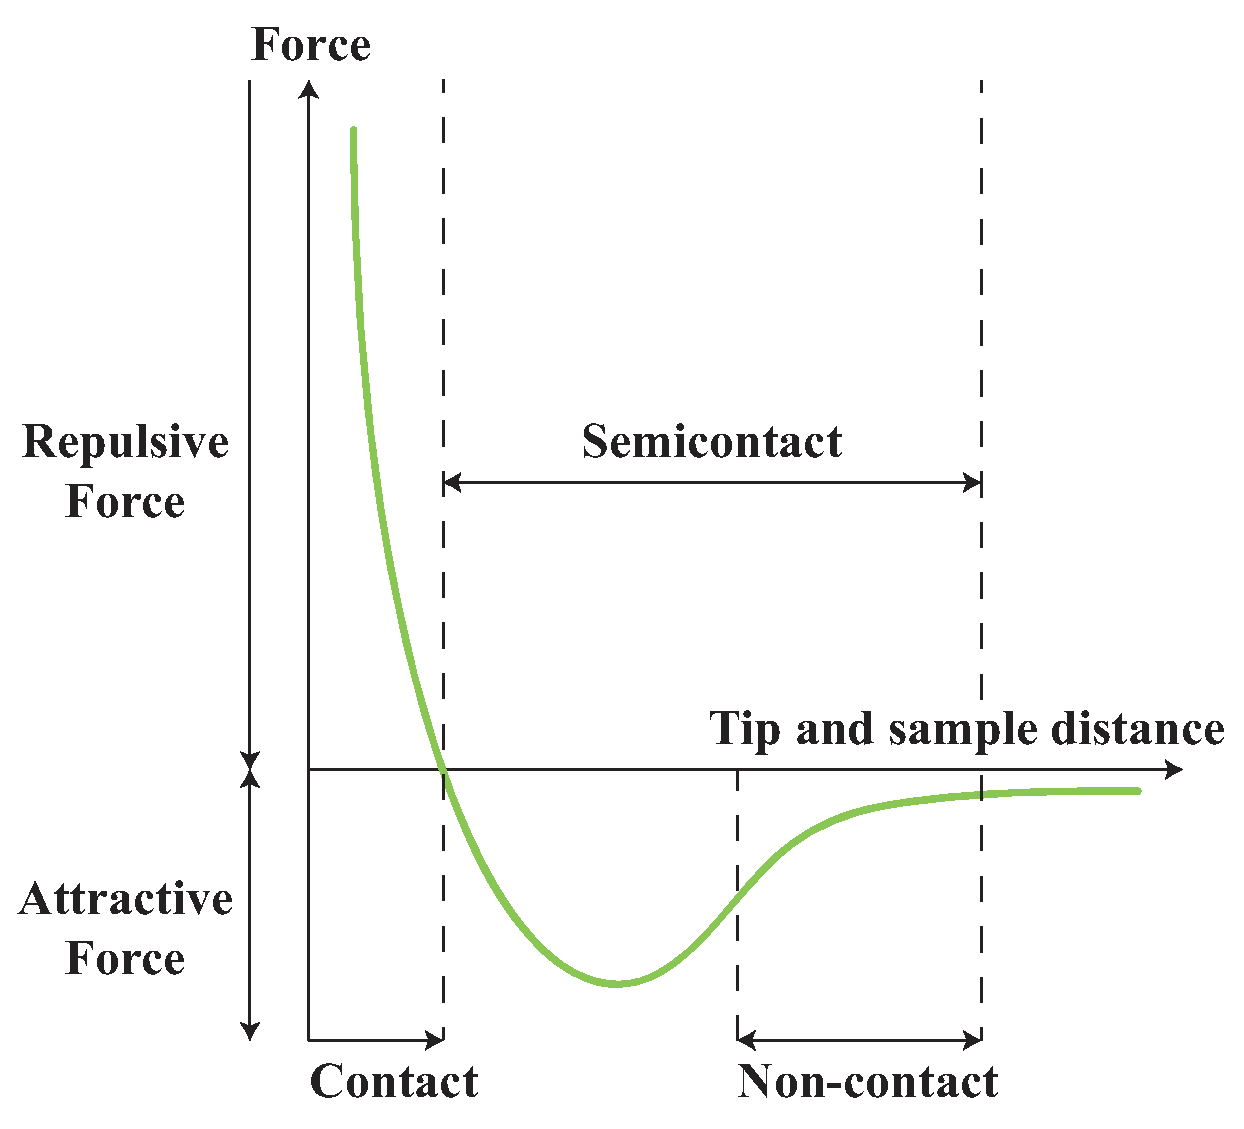
\includegraphics[scale=0.6]{EXP/afm3.eps}
\caption{\label{fig:afm3}Sketch of tip-sample forces.}
\end{figure}

\paragraph{Contact mode}

In contact mode of operation the cantilever deflection under scanning reflects repulsive force acting upon the tip. Repulsion force $\mathbf{F}$ acting upon the tip is related to the cantilever deflection value $\mathbf{x}$ under Hooke's law: $\mathbf{F}=-K \cdot  \mathbf{x}$, where $K$ is cantilever spring constant. The spring constant values for different cantilevers usually vary from 0.01 to several $\mathbf{N/m}$.

In our units the vertical cantilever deflection value is measured by means of the optical registration system and converted into electrical signal DFL (difference signal between the upper and lower halves of the PSPD) . In contact mode the DFL signal is used as a parameter characterizing the interaction force between the tip and the surface. There is a linear relationship between the DFL value and the force. In constant force mode of operation the deflection of the cantilever is maintained by the feedback circuitry on the preset value. So vertical displacement of the scanner under scanning reflects topography of sample under investigation.

Contact force microscopy is surface topography measurement in the contact mode.The microscope operation in the mode of maintaining constant interaction force between the tip and the surface sample, and is the base for measuring surface topography as well as for measuring local rigidity, local viscosity and local friction force. Constant force mode has some advantages and disadvantages. Main advantage of constant force mode is possible to measure with high resolution simultaneously with topography and some other characteristics, such as friction forces, spreading resistance etc. Constant force mode has also some disadvantages. Speed of scanning is restricted by the response time of feedback system. When exploring soft samples they can be destroyed by the scratching because the probe scanning tip is in direct contact with the surface. Therefore, under scanning soft unhomogeneous samples the local flexure of sample surface varies. As a result acquired topography of the sample can be proved distorted. Possible existence of substantial capillary forces imposed by a liquid adsorption layer can decrease the resolution.

\paragraph{Semi-contact mode}

The semi-contac mode can be characterized by some advantages in comparison with contact mode. First of all, in this mode the force of pressure of the cantilever onto the surface is less, that allows to work with softer materials such as polymers and bio-organics. The semi contact mode is also more sensitive to the interaction with the surface that gives a possibility to investigate some characteristics of the surface distribution of magnetic and electric domains, elasticity and viscosity of the surface. 

Widely used semi-contact mode has some disadvantage concerned with the usage of the feedback circuit. The scanning speed in semi-contact mode is restricted by the feedback circuit reaction time. This disadvantage can be overcome by the fact that under scanning new value of cantilever oscillation amplitude (and error signal) usually is achieved faster than preset value of the cantilever oscillation amplitude can be reached by the feedback system. Time of the reaching new value of the oscillation amplitude is determined by the oscillation period and Q-quality of the cantilever.
The feedback error signal, emerging when scanning in the semi-contact mode, contains some additional information about the topography. It can be utilized for achieving a more precise recovery of the relief. 

Additionally, similarly to the contact error mode, which can be considered as intermediate between the constant force mode and constant height mode, the feedback gain factor (i.e. the feedback processing speed) can be adjusted for the system to be able to trace subtle changes of the relief and to be too slow to trace the steep changes. Then, when the probe travels over minor irregularities, scanning will be carried out with an almost constant piezo scanner length. As a result, the slow changes of the relief will hardly show up on the images, and the steep changes will appear in high contrast. This may be helpful in finding minor irregularities on large areas against major sloping relief features. It must be noted that height of the minor irregularities must be less than amplitude of cantilever oscillation.

\section{Scanning electron microscopy}

The scanning electron microscope (SEM) is used for the observation of specimen surfaces~\cite{von1938elektronen}. When the specimen is irradiated with a fine electron beam, secondary electrons are emitted from the specimen surface. Topography of the surface can be observed by two-dimensional scanning of the electron probe over the surface and acquisition of an image from the detected secondary electrons. The concept schematic of commercial SEM (JEOL, JSM-6500F) is shown in Figure~\ref{fig:sem1}. The basic unit is composed of an electron optical system, a specimen stage, a secondary-electron detector, an image display unit, and an operation system. The electron optical system consists of an electron gun, a condenser lens and an objective lens to produce an electron probe, a scanning coil to scan the electron probe, and other components. The system inside of the microscope column are kept at vacuum.
\begin{figure}[htb]
\centering
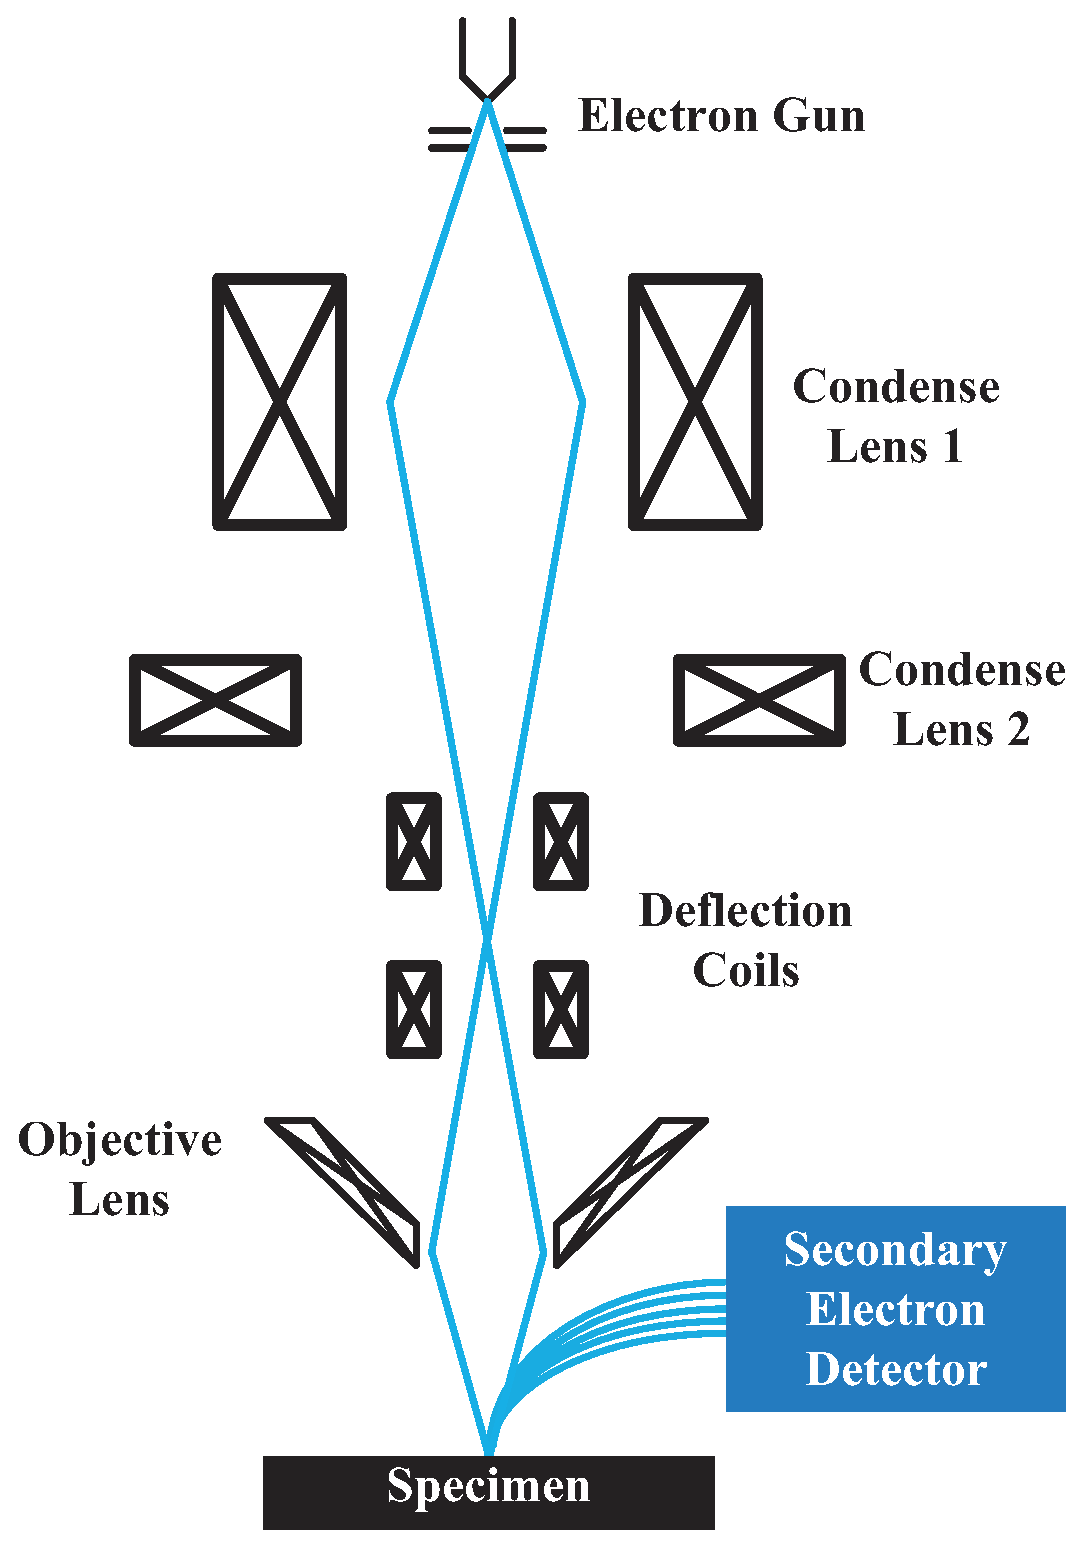
\includegraphics[scale=0.5]{EXP/SEM.eps}
\caption{\label{fig:sem1}Basic construction of a scanning electron microscopy.}
\end{figure}


The JSM-6500F utilizes a Schottky type field-emission (T-FE) gun for the electron source. The T-FE gun can constantly supply the surface of the cathode with zirconium oxide by heating the surface of cathode to 1800 K. For this reason, it can easily obtain stable and high probe current (range from several pA to 100 nA) compared with the traditional thermal emission electron gun and cold field-emission gun.

The magnetic condenser and objective lens system act to control the diameter of the beam as well as to focus the beam on the specimen due to a rotationally-symmetric magnetic field is formed when we pass a direct electric current through a coilwound electric wire in the magnetic lens. A pair of deflector coils, which between the condenser and objective lens, controlled by the scan generator, which are responsible for rastering that focused beam across the specimen surface. The size of the rastering pattern is under magnification control. The beam is rastered from left to right and top to bottom. There is a one-to-one correspondence between the rastering pattern on the specimen and the rastering pattern used to produce the image on the monitor. The resolution we choose to image at will obviously affect the number of pixels per row as well as the number of rows that constitute the scanned area.

The signal is generated from the specimen, and collected by the detector and subsequently processed to generate the image. That processing takes the intensity of the signal coming from a pixel on the specimen and converts it to a grayscale value of the corresponding monitor pixel. The monitor image is a two dimensional rastered pattern of grayscale values.

With the beam focused on the specimen surface, all we need to do to change magnification is to change the size of the rastered area on the specimen. The size of the monitor raster pattern is constant. Magnification will increase if we reduce the size of the area scanned on the specimen.

%\bibliographystyle{unsrt}
%\bibliography{thesisbib}
%\include{main}
%\include{conclusions}

%---------- Input your reference here ---------
\bibliographystyle{myieeetr}
\addcontentsline{toc}{chapter}{\bibname}
\nocite{*}
\bibliography{thesisbib}

%----------- Input your appendix here  -----------
\appendix
%\chapter{First appendix title}

Open and edit \href{run:./AppendixA.tex}{AppendixA.tex} 
%or %chapter cite  == \include
%\chapter{First appendix title}

Open and edit \href{run:./AppendixA.tex}{AppendixA.tex}
\begin{appendices}
\chapter{Software Tools Used in This Research} \label{chap:sw} 
%%\framebox{REVIEW1}
This research won't come into reality without many free and open-source software tools and free resources, we will walk you through a brief introduction to the softwares we used in this research. 
\section*{Linux Operating System}
Most of the tools introduced below runs on modern Linux distributions. The distribution we are using is \textbf{Linux Mint Debian Edition (LMDE)}\footnote{\url{http://www.linuxmint.com/download_lmde.php}} (Linux kernel 3.10), which is a user-friendly Linux distribution based on Debian Testing. User who want to try music-related softwares without installing Linux on their harddrive can try \textbf{64 Studio}\footnote{\url{http://www.64studio.com/}} Linux, which is a live CD distribution with many music-related software pre-installed. It also has many kernel optimizations for real-time music manipulation. \textbf{Ubuntu Studio}\footnote{\url{http://ubuntustudio.org/}} is also an option, which has many pre-installed music softwares and is based on the popular Ubuntu Linux.

Many Linux distributions use PulseAudio audio server to manage audio device. But a badly configured PulseAudio server will introduce severe latency, which is not acceptable while doing MIDI recording. One workaround is to remove PulseAudio and use raw ALSA (Advanced Linux Sound Architecture) driver instead. But be careful, hardware volume keys may not work without PulseAudio. 

\section*{Programming Languages}
   \section*{Python}
   Many researcher will choose Matlab or Octave for scientific projects because they have many useful toolboxes included. However, we believe that research project \enquote{doesn't exist in vacuum}. Drawing insight from the famous 80-20 rule, only 20\% of the code are actually doing the core algorithm, the rest 80\% are doing file manipulation, configuration, user interaction, and visualization. Therefore, choosing a powerful and easy to write general-purpose programming language is extremely crucial. \textbf{Python}\footnote{\url{https://www.python.org/}} construct most of the infrastructure code for this project. Python is super easy to code, and has almost every tool you need to construct a fully functional experiment environment. We will highlight some useful module:
   \subsection*{\texttt{Music21}\footnote{\url{http://web.mit.edu/music21/}}}
   We would like to give special thanks to the \texttt{music21} developemnt team. \texttt{Music21} is a python toolbox for music notation manipulation and analysis, developed by MIT. \texttt{Music21} can parse many score notations like MusicXML, MIDI\footnote{By default, \texttt{music21} will quantize MIDI input, so if you want to import MIDI recorded from human performance, you need to bypass the default parser and manually disable the quantizer.} and more into a very convenient \texttt{music21} object data structure. Researcher can easily filter, split, search, and transform music notations. There are also many music analysis routines and feature extractors included. If you want to do computer music research, \texttt{music21} is a god-sent resource. 
   \subsection*{SciPy, NumPy and Matplotlib\footnote{\url{http://www.scipy.org/}}}
   SciPy is a project that contains many useful toolboxes for scientific computation in Python. The SciPy core library and NumPy provides numerical and vector calculation for Python, with similar capability to Matlab. Matplotlib provides plotting tools also similar to Matlab. It's useful for small scale calculation, but heavy duty mathematical calculation, we suggest \texttt{R} programming language, which will be discussed in later section.

   \subsection*{\texttt{Simplejson}}
   JSON (JavaScript Object Notation) is a plaintext data-interchange format, similar to XML but much light-weight. JSON is useful in experiment code for two purpose: first, JSON can serve as configuration file, it easy to parse and easy to edit. Second, JSON can serve as intermediate data file between each experiment module. For example, we use JSON to send extracted features from feature extractors to the machine learning module. Although plaintext takes more storage than binary file, but it's much easier to debug because it's human readable. And you can simply parse the intermediate values and plot it using other plotting program. Python provides build-in support for JSON format via \texttt{json} and \texttt{simplejson} packages.

   \subsection*{\texttt{Argparse}}
   \texttt{Argparse} provides command line argument parser for python scripts, using commandline arguments with configuration file in JSON, you can create very flexible, extendible scripts that are easy to automate.

   \subsection*{\texttt{Logging}}
   The built in \texttt{logging} module can print logging information with predefined format, and it supports log level. By using log level, you can print debug information during development, and hide all debug message during production simply by changing the log level flag.

   \section*{\texttt{R}\footnote{\url{http://www.r-project.org/}}}
   \texttt{R} is a programming language for statistical calculation, but it can also do general purpose math and plotting very well. \texttt{R} follows a functional programming design, so it may take some time to learn for people who only have experience in C/C++, Java or other imperative and/or Object-oriented programming language. But it is a great tool for statistical computation, data analysis and visualization. We use R for experiment data analysis and for linear regression in early version of this research. \texttt{R} and Python can work seamlessly through the \texttt{rpy} package.

\section*{Score Manipulation and Corpora}
\subsection*{MusicXML and MuseScore}
\textbf{MusicXML}\footnote{\url{http://www.musicxml.com/}} is a digital score notation format based on XML. It is well supported in most commercial music typesetting software. %For other music typesetting format you may want to look at LilyPound. 
To view and edit musicXML score, we use the open-source software \textbf{MuseScore}\footnote{\url{http://musescore.org/}}, it provides basic editing capability, and can export score as PDF. However, MuseScore often crash while loading bad-formatted musicXML file, so sometimes you need to look into it log file and fix the ill-formated XML via a text editor.
\subsection*{Corpora}
\texttt{Music21} contains a corpus\footnote{\url{http://web.mit.edu/music21/doc/systemReference/referenceCorpus.html}}, which will be automatically installed if you accept the licence term during \texttt{music21} installation. It covers a wide range of composers from early music, classical music to folk songs, with various genre and musical style. Another public available corpus is called \textbf{KernScore}\footnote{\url{http://kern.ccarh.org/}}, which provides a better search engine. You can find works by composer, genre, form or other criteria. There are even a special section containing monophonic works. Scores from both corpus can be loaded and transformed in to desired format via \texttt{music21}.

\section*{MIDI Recording}
\textbf{Rosegarden}\footnote{\url{http://www.rosegardenmusic.com/}} is a digital audio workstation (DAW) software designed specifically for MIDI. It can record, edit, mix and export MIDI tracks. To actually hear the music, you need a MIDI synthesizer to work with Rosegarden. \textbf{Timidity++}\footnote{\url{http://timidity.sourceforge.net/}} is built-in in many Linux distribution, and it provides a commandline interface to synthesize MIDI directly into a WAV file. However, the default sound quality from Timidity++ is not very satisfying, so we suggest qSynth, which is a QT front end for \textbf{FluidSynth}\footnote{\url{http://sourceforge.net/projects/fluidsynth/}}. The default soundfont that comes with FludiSynth has very good sound quality.

With all these music software, it will soon be very hard to control the interconnection between programs. This is when \textbf{JACK}\footnote{\url{http://jackaudio.org/}} comes to help. JACK is like a virtual \enquote{plug-board} for software that implements the JACK interface. It provides a central place in which you can control how the music data flows between programs and hardware.

\section*{Audio Manipulation}

When MIDI files are synthesized into WAV format, there are many tools that can help editing them. The most easy to use software with GUI is \textbf{Audacity}\footnote{\url{http://audacity.sourceforge.net/}}, it can edit and mix audio tracks. For commandline tools (in case you need automation), \textbf{oggenc}\footnote{\url{http://www.vorbis.com/}}(ogg vorbis encoder), \textbf{lame}\footnote{\url{http://lame.sourceforge.net/}}(MP3\footnote{Please consider open format like ogg first, MP3 is a closed format and may have patent issues.} encoder) and \textbf{FFmpeg}\footnote{\url{http://www.ffmpeg.org/}} are very helpful for file format transformation. To cut and combine audio tracks from commandline, use \textbf{SoX}\footnote{\url{http://sox.sourceforge.net/}}.

\section*{Data Visualization}
As mentioned before, \texttt{R} and \texttt{Matplotlib} are good candidate for visualizing experiment data. But if you don't want to learn the syntax of R or Python, you can try \textbf{gnuplot}\footnote{\url{http://www.gnuplot.info/}}. Gnuplot is a interactive (and scriptting) environment for generating various types of plot like line plots or bar charts. It works particularly well if you use \texttt{grep} to extract data for many files, say, extracting execution time information from logs.

\section*{SVM\textsuperscript{hmm}}
SVM\textsuperscript{hmm}\footnote{\url{http://www.cs.cornell.edu/people/tj/svm_light/svm_hmm.html}} is an implementation for structural support vector machine with hidden Markov model output. It's developed by Thorsten Joachims from Cornell University. It is based on SVM\textsuperscript{struct}, a more general framework for structural support vector machine. There are many other SVM\textsuperscript{struct} extensions such as Python or Matlab API.
   

\section*{Other}
Sometimes the machine learning algorithm will run for a very long time. Then it's better if you can find a server that runs 24-7 in your home or laboratory. You can install a \textbf{ssh} server on that machine, and controls the experiment execution remotely. However, the experiment program will be terminated once you log out the \texttt{ssh} session. You can run your experiment program in \textbf{tmux}\footnote{\url{http://tmux.sourceforge.net/}}, a terminal multiplexer, instead. It will keep your program running even if you log out of your SSH session.

Modern machines often have multi-core CPUs. But if your program only runs in one core, you waste the CPU resources and also your time. \textbf{Gnu-parallel}\footnote{\url{http://www.gnu.org/software/parallel/}} can dispatch multiple instances of your script or program to each core. It will automatically find new job to run when the previous one is finished, so the CPU will always run on its full capacity. 

Finally, We use \textbf{git}\footnote{\url{http://git-scm.com/}} for version control (including code and document). And \LaTeX\footnote{\url{http://latex-project.org/}} is used to typeset this document.

\section*{Summary}
We have reviewed many software tools used to construct this research. We want to emphasize that it is totally possible to use \textit{only} free and open-source software to do all these heavy lifiting. We encourge the reader to try these tools out, spread the words and even contribute to these projects. By doing so we can create a more friendly scientific computing community and make the world a better place.

%\chapter{Using the Expressive Performance Corpus}

%
\chapter{Guide}
 這裡將簡單介紹如何利用\LaTeX\ 來編輯你的畢業論文,若不知道\LaTeX\ 是什麼或是沒有概念的話,建議你可以簡單看過放在此資料夾裡的\href{run:./latex123.pdf}{李果正-大家來學\LaTeX}前四章內容,在下載適合的\LaTeX\ 整合發行套件之後(請看第~\ref{it:download}項),可以嘗試用剛安裝好的\LaTeX\ 編輯器來編譯\href{run:./thesis.tex}{thesis.tex}這份文件,編譯的方法可以看下面第~\ref{it:comp}項的介紹,若編譯成功,所編譯出來的thesis.pdf文件的應該會跟此demo.pdf文件一模一樣,而且沒有任何問號符號,走到這一步的話,就差不多可以開始邊學習\LaTeX\ 邊編輯你的畢業論文了!基本上會使用到的指令都包含在論文的的各章節裡,怎麼在論文裡寫公式或是放圖之類的就自行看tex檔學吧。如果有任何問題或建議可以來信與我討論,我的信箱是\href{mailto:dran31545@gmail.com}{dran31545@gmail.com},或是到此範本\href{http://code.google.com/p/ntu-thesis-latex-template/}{Google Project}裡面的\href{http://code.google.com/p/ntu-thesis-latex-template/issues/list}{Issues}貼上你的問題與建議,我會盡我所能更新此範本,也歡迎大家自行重製、改良此範本並散布給他人,祝大家順利畢業!\\\\
 要編輯致謝請打開\href{run:./acknowledgementsCH.tex}{acknowledgementsCH.tex}\\
 \begin{enumerate}[leftmargin=0pt, topsep=0pt, itemsep=0pt, label=\Roman{*}.]
\item 此範本參考並修改自下列網站的資料:
\begin{enumerate}[topsep=0pt, itemsep=0pt, label=$\bullet$]
    \item \href{http://www.csie.ntu.edu.tw/~tzhuan/www/resources/ntu/}{如何用 LaTeX 排版臺灣大學碩士論文}\\
    \textemdash 台灣大學論文\LaTeX\ 樣版原創者\href{http://www.csie.ntu.edu.tw/~tzhuan/www/}{黃子桓}的教學網頁
    \item \href{http://www.hitripod.com/blog/2012/05/latex-thesis-template-quick-reference/}{LaTeX 常用語法及論文範本}\\
    \textemdash \href{http://www.hitripod.com/blog/}{Hitripod}所修改的範本,這裡參考了許多他所寫的格式和內容
    \item \href{http://www.cc.ntu.edu.tw/chinese/epaper/0014/20100920_1404.htm}{使用LaTeX做出精美的論文}
    \item \href{http://www.hitripod.com/blog/2011/04/xetex-chinese-font-cjk-latex/}{XeTeX:解決 LaTeX 惱人的中文字型問題}
    \item \href{http://code.google.com/p/ntuthesis/}{台灣大學碩士、博士論文的Latex模板}\\
\end{enumerate}
\item 幾個有用的參考資料及網路資源:
\begin{enumerate}[topsep=0pt, itemsep=0pt, label=$\bullet$]
    \item \href{run:./latex123.pdf}{李果正-大家來學\LaTeX}\textemdash 建議先看完前四章
    \item \href{http://en.wikibooks.org/wiki/LaTeX}{WIKIBOOKS-\LaTeX}\textemdash 好用的線上工具書
    \item \href{run:./Working_with_a_bib_file_using_Jabref.pdf}{Working with a .bib file using JabRef}
    \item \href{run:./Fi087_S.pdf}{Using BibDesk - A short tutorial}
    \item \href{http://www.dfcd.net/articles/latex/latex.html}{LaTeX for Physicists}\\
\end{enumerate}
\item 下載\LaTeX\ 整合發行套件,可參考\href{http://www.tug.org/texcollection/}{TeX Collection}:\label{it:download}
 \begin{enumerate}[topsep=0pt, itemsep=0pt, label=\arabic{*}.]
     \item \href{http://www.tug.org/mactex/}{MacTeX}: For \textcolor{Green}{\textbf{MacOSX}},下載\href{http://mirror.ctan.org/systems/mac/mactex/MacTeX.pkg}{MacTeX.pkg}
     \item \href{http://www.tug.org/protext/}{ProTeXt}: For \textcolor{Green}{\textbf{Windows}},下載\href{ftp://ftp.fernuni-hagen.de/pub/windows/win32/ProTeXt/}{ISO file}
     \item \href{http://www.tug.org/texlive/}{TeX Live}: For \textcolor{Green}{\textbf{GNU/Linux}} and \textcolor{Green}{\textbf{MacOSX}}, and \textcolor{Green}{\textbf{Windows}},下載\href{http://www.tug.org/texlive/acquire-iso.html}{ISO file}
     \item \href{http://ctan.org/}{CTAN}: The Comprehensive TeX Archive Network.\\
 \end{enumerate}

\item 好用的程式:
 \begin{enumerate}[topsep=0pt, itemsep=0pt, label=$\bullet$]
    \item 文獻管理系統:
        \begin{enumerate}[topsep=0pt, itemsep=0pt, label=\arabic{*}.]
         \item \href{http://jabref.sourceforge.net/}{JabRef}\\
                     可參考\href{run:./Working_with_a_bib_file_using_Jabref.pdf}{Working with a .bib file using JabRef}或是\href{https://www.google.com/search?q=jabref}{Google}及\href{http://www.youtube.com/results?search_query=jabref}{YouTube}
         \item \href{http://bibdesk.sourceforge.net/}{BibDesk} (For Mac)\\
                     可參考\href{run:./Fi087_S.pdf}{Using BibDesk - A short tutorial}或是\href{https://www.google.com/search?q=bibdesk}{Google}及\href{http://www.youtube.com/results?search_query=bibdesk}{YouTube}
         \end{enumerate}
         \item 方程式編輯器:\href{https://chrome.google.com/webstore/detail/dinfmiceliiomokeofbocegmacmagjhe?hl=zh-TW}{Daum Equation Editor} (Chrome App,必須使用Google瀏覽器)\\
 \end{enumerate} 
\item 編譯流程:\label{it:comp}
\begin{enumerate}[topsep=0pt, itemsep=0pt, label=\arabic{*}.]
    \item \texttt{xelatex thesis}\\ 對thesis.tex進行第一次XeLaTeX編譯,產生thesis.pdf以其他檔案
    \item \texttt{bibtex thesis}\\ 對thesis.tex進行BibTeX編譯,產生bbl檔以及blg檔
    \item \texttt{xelatex thesis}\\ 對thesis.tex進行第二次XeLaTeX編譯,產生目錄、圖表連結及參考文獻
    \item \texttt{xelatex thesis}\\ 對thesis.tex進行第三次XeLaTeX編譯,產生參考文獻連結,完成編譯
\end{enumerate} 
    \textcolor{Red}{注意!}此範本使用cite套件,可依據你利用文獻管理系統所整理好的\href{run:./thesisbib.bib}{thesisbib.bib}檔在論文最後產生參考文獻頁面,若你的系所規定要在每個章節的後面產生參考文獻,則可以用chapterbib套件,來對每個有附參考文獻的章節tex檔進行一次BibTeX編譯產生bbl檔,如範例的\href{run:./introduction.tex}{introduction.tex}、\href{run:./THM.tex}{THM.tex}和\href{run:./EXP.tex}{EXP.tex},如果有這需要請把\href{run:./thesis.tex}{thesis.tex}檔裡使用cite套件的指令利用註解符號\texttt{\%}來取消使用cite套件,並刪去出現在使用chapterbib套件指令前面的註解符號\texttt{\%}來啟動使用chapterbib套件
    \begin{verbatim}
\usepackage{cite}
%\usepackage{chapterbib}
改成
%\usepackage{cite}
\usepackage{chapterbib}
    \end{verbatim}
    再來利用註解符號\texttt{\%}取消會把參考文獻放在論文最後的指令
    \begin{verbatim}
\bibliographystyle{unsrt}
\addcontentsline{toc}{chapter}{\bibname}
\bibliography{thesisbib}
改成
%\bibliographystyle{unsrt}
%\addcontentsline{toc}{chapter}{\bibname}
%\bibliography{thesisbib}
    \end{verbatim}
    再把用來輸入章節檔案的\texttt{\textbackslash input}指令改成\texttt{\textbackslash include}指令
     \begin{verbatim}
\chapter{Introduction}
\framebox{REVIEW1}
\section{Motivation}
%Robot => speech => MIDI (history)
From the machnical music performing antomata, to the Japanese virtual signer Hatune Miku, there had been many attempts to create autoated system that performs music. However, many of these system can only perform predefined expression, which is not very satisfying. State-of-the-art text-to-speech system can already generate fluid and natural speech, but computer performance still can't perform very expressivly.

Therefore, many researcher have devoted many effort to develop systems that can automatically or semi-automatically perform music expressively. There is even a biannual contest called Music Performance Rendering Contest (RenCon)\cite{RenCon} that puts all performance system to into competition. Their roadmap suggest that they wish to win the Chopin International Piano Contest by a computer perforer. We will review previous works, including many which won the RenCon prizes, in Chapter \ref{chap:prev}.
%Computer generated music, such as synthsized MIDI, are often considered robotic and unexpressive. But we have already witnessed the fluid and lively sound generated by state-of-the-art text-to-speech systems. This inspired us to develop a system that can read a music score and play it in an expressive, humanly way. Such system can be used for audiolizing score notation editing software, creating interactive media content, and generating royality-free music. 

%Established pianists always has his/her own distinctive style. Such sytle distinguised himself/herself from all the other pianists. If the expressive performance system can learn the style of a performer, it might be able to provide musicological insight of performance styles. Furthermore, we can even make a mastero who is no longer with us play music he/she never played in his/her lifetime.

There are many applications for a computer expressive performance system, many commercial music typesetting software like Finale and Sibelius already have expressive playback features built-in. On the commercial side, such system can provide personalized music listening experience. For the music production industry, it saved a lot of cost on hiring musicians or licensing. Such system can also opens up new opportunity in music making, such as human-machine co-performance, or interactive multimedia installation. In academia, researchers can use this technology to model the performing style of musicians, or restore historical music archive.

\framebox{TODO:Discuss Mazolla's theroy of expressive performance}

%\begin{figure}[tp]
%   \begin{center}
%      %TODO:Fig.: expressive performance concept
%      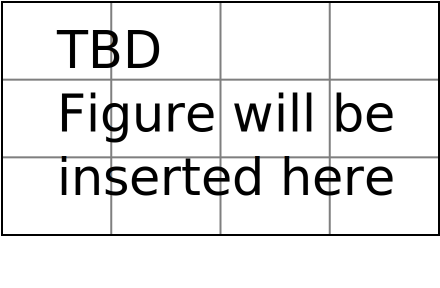
\includegraphics[width=\textwidth]{fig/TBDFigure}
%
%   \end{center}
%   \caption{From Composer to Performance}
%   \label{fig:concept}
%\end{figure}
%Application: musicology study, typesetting tool, play score archive, play computer-generated music, accompaniment



\section{Goal and Contribution}
\framebox{TODO:brief guide to previous works}
There are many different goals for computer expressive performance, which will be discussed in Chapter \ref{chap:prev}. In this research the ultimate goal is to be able to play any music in any expressive style specified. But due to the technical and time constrain, we need to set a more practical goal for our research. We wish to build a computer expressive performance system based on an offline supervised learning algorithm. The system will be able to learn any play monophonic musical phrases. The expressiveness will be at phrase level, structural or timbre related expression are not the primary concern. The performance style will be controlled by the learning material, which is traditional music notation, with human-annotated phrasing information. If only recordings from a single performer is given, it should learn the particular style of the performer.


The major contribution of this thesis is that we apply structural support vector machine on expressive performance problem. There exist no previous work that uses the discriminative learning power of support vector machine on computer expressive performance question. We also developed methods and tools to generate corpus for expressive performance system based on learning algorithms. 
%\bibliographystyle{unsrt}
%\bibliography{thesisbib}
\section{Chapter Organization}
In Chapter \ref{chap:prev}, we will give an overview of previous works and their varying goals, the works will be grouped by the way they learn performance knowledge, and finally we will discuss some additional specialities such as special instrument model or special user interaction pattern. In Chapter \ref{chap:proposed}, we will first give a brief introduction to the mathematical background of the learning algorithm, SVM-HMM. And then we will provide a top-down explanation to the proposed method. Then in Chapter \ref{chap:corpus}, we will explain how the corpus used for training is designed and implemented. Finally, In Chapter \ref{chap:exp}, we will show several experiment results and discussions. We have also included two appendixes, appendix \ref{chap:sw} presents some software tools used in this research, which may be helpful for other researchers in music and machine learning fields.
  =>  \chapter{Introduction}
\framebox{REVIEW1}
\section{Motivation}
%Robot => speech => MIDI (history)
From the machnical music performing antomata, to the Japanese virtual signer Hatune Miku, there had been many attempts to create autoated system that performs music. However, many of these system can only perform predefined expression, which is not very satisfying. State-of-the-art text-to-speech system can already generate fluid and natural speech, but computer performance still can't perform very expressivly.

Therefore, many researcher have devoted many effort to develop systems that can automatically or semi-automatically perform music expressively. There is even a biannual contest called Music Performance Rendering Contest (RenCon)\cite{RenCon} that puts all performance system to into competition. Their roadmap suggest that they wish to win the Chopin International Piano Contest by a computer perforer. We will review previous works, including many which won the RenCon prizes, in Chapter \ref{chap:prev}.
%Computer generated music, such as synthsized MIDI, are often considered robotic and unexpressive. But we have already witnessed the fluid and lively sound generated by state-of-the-art text-to-speech systems. This inspired us to develop a system that can read a music score and play it in an expressive, humanly way. Such system can be used for audiolizing score notation editing software, creating interactive media content, and generating royality-free music. 

%Established pianists always has his/her own distinctive style. Such sytle distinguised himself/herself from all the other pianists. If the expressive performance system can learn the style of a performer, it might be able to provide musicological insight of performance styles. Furthermore, we can even make a mastero who is no longer with us play music he/she never played in his/her lifetime.

There are many applications for a computer expressive performance system, many commercial music typesetting software like Finale and Sibelius already have expressive playback features built-in. On the commercial side, such system can provide personalized music listening experience. For the music production industry, it saved a lot of cost on hiring musicians or licensing. Such system can also opens up new opportunity in music making, such as human-machine co-performance, or interactive multimedia installation. In academia, researchers can use this technology to model the performing style of musicians, or restore historical music archive.

\framebox{TODO:Discuss Mazolla's theroy of expressive performance}

%\begin{figure}[tp]
%   \begin{center}
%      %TODO:Fig.: expressive performance concept
%      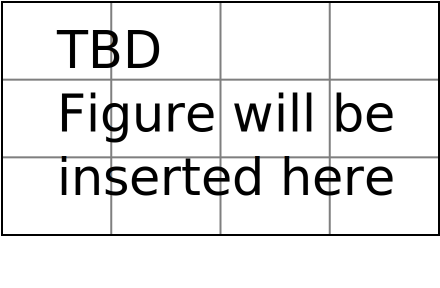
\includegraphics[width=\textwidth]{fig/TBDFigure}
%
%   \end{center}
%   \caption{From Composer to Performance}
%   \label{fig:concept}
%\end{figure}
%Application: musicology study, typesetting tool, play score archive, play computer-generated music, accompaniment



\section{Goal and Contribution}
\framebox{TODO:brief guide to previous works}
There are many different goals for computer expressive performance, which will be discussed in Chapter \ref{chap:prev}. In this research the ultimate goal is to be able to play any music in any expressive style specified. But due to the technical and time constrain, we need to set a more practical goal for our research. We wish to build a computer expressive performance system based on an offline supervised learning algorithm. The system will be able to learn any play monophonic musical phrases. The expressiveness will be at phrase level, structural or timbre related expression are not the primary concern. The performance style will be controlled by the learning material, which is traditional music notation, with human-annotated phrasing information. If only recordings from a single performer is given, it should learn the particular style of the performer.


The major contribution of this thesis is that we apply structural support vector machine on expressive performance problem. There exist no previous work that uses the discriminative learning power of support vector machine on computer expressive performance question. We also developed methods and tools to generate corpus for expressive performance system based on learning algorithms. 
%\bibliographystyle{unsrt}
%\bibliography{thesisbib}
\section{Chapter Organization}
In Chapter \ref{chap:prev}, we will give an overview of previous works and their varying goals, the works will be grouped by the way they learn performance knowledge, and finally we will discuss some additional specialities such as special instrument model or special user interaction pattern. In Chapter \ref{chap:proposed}, we will first give a brief introduction to the mathematical background of the learning algorithm, SVM-HMM. And then we will provide a top-down explanation to the proposed method. Then in Chapter \ref{chap:corpus}, we will explain how the corpus used for training is designed and implemented. Finally, In Chapter \ref{chap:exp}, we will show several experiment results and discussions. We have also included two appendixes, appendix \ref{chap:sw} presents some software tools used in this research, which may be helpful for other researchers in music and machine learning fields.

\chapter{Theory of surface plasmon polaritons in metallic nano-structures}
\label{c:thm}
\section{Definition of plasmon}

Plasmon is collective oscillation of conduction electron gas, a quasi-particle resulting from the quantization of plasma oscillations just like phonons are quantizations of mechanical vibrations. The simplest case is the volume plasmon as shown in Figure~\ref{fig:bulk}.
\begin{figure}[htb]
\centering
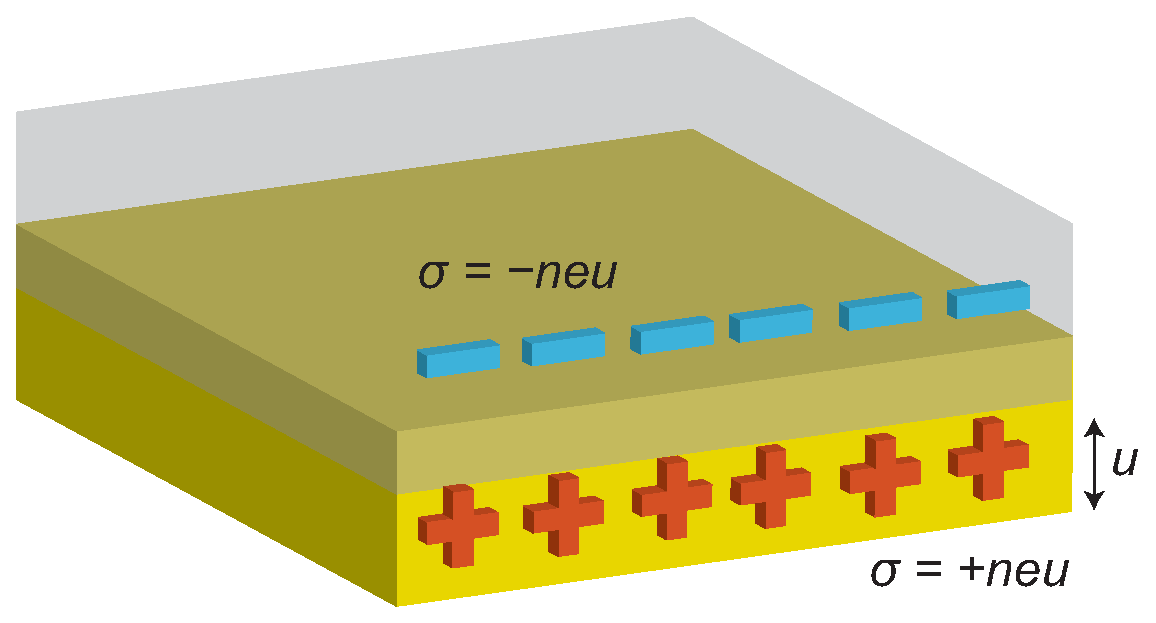
\includegraphics[scale=0.5]{THM/bulk.eps}
\caption{\label{fig:bulk}Longitudinal collective oscillations of the conduction electrons of a metal (Volume plasmons)}
\end{figure}
 We can derive plasma frequency $\omega_p$ from the simple harmonics oscillation model, a collective displacement of the electron cloud by a distance $u$ leads to a surface charge density $\sigma = \pm neu$ at the slab boundaries. This establishes a homogeneous electric field $\mathbf{E} = \frac{neu}{\varepsilon_0}$ inside the slab. Thus, the displaced electrons experience a restoring force, and their movement can be described by the equation of motion $nm\ddot{u} = -ne\mathbf{E}$. Inserting the expression for the electric field, this leads to
 \begin{subequations}
 \begin{align}
 nm\ddot{u} = -\frac{n^2e^2u}{\varepsilon_0} \\
 \ddot{u} + {\omega_p}^{2}u = 0\text{.}
 \end{align}
 \end{subequations}
  The plasma frequency $\omega_p = \sqrt{\frac{ne^2}{\varepsilon_0m}}$ can thus be recognized as the natural frequency of a free oscillation of the electron sea. The quanta of these charge oscillations are called plasmons. Due to the longitudinal nature of the excitation, volume plasmons do not couple to transverse electromagnetic waves, and can only be excited by particle impact. We can derive the dispersion relation of the generalization of volume plasmons, traveling plasma waves, from curl electric field equations (Equations~\ref{eq:curlE})
 \begin{subequations}
 \begin{align}
 \curl{\curl \mathbf{E}} &= -\mu_0 \frac{\partial^2\mathbf{D}}{\partial t^2}\label{eq:curlE}\\
\mathbf{K}( \mathbf{K}\cdot \mathbf{E}-K^{ 2 }\mathbf{E} ) &=-\varepsilon ( \mathbf{K},\omega  ) \frac { { \omega  }^{ 2 } }{ { c }^{ 2 } } \mathbf{E}
 \end{align}
 \end{subequations}  
and plasma model, and a simple equation of motion for an electron of the plasma subjected to an external electric field $\mathbf{E}$
 \begin{equation}
m\ddot{\mathbf{x}} + m\gamma\dot{\mathbf{x}} = -e\mathbf{E}\text{.}
\end{equation}
Assuming a harmonic time dependence $\mathbf{E}( t )=\mathbf{E}_0\mathrm{e}^{-i\omega t}$ of the driving field, a particular solution of this equation describing the oscillation of the electron is $\mathbf{x} ( t ) = \mathbf{x}_0 \mathrm{e}^{-i\omega t} $. The complex amplitude $\mathbf{x}_0$ incorporates any phase shifts between driving field and response via
\begin{equation}
\mathbf{x} ( t ) = \frac{e}{m( \omega^2 + i\gamma\omega )}\mathbf{E}( t )\text{.}
\end{equation}
The displaced electrons contribute to the macroscopic polarization
\begin{equation}
\mathbf{P}=-\frac{ne^2}{m( \omega^2 + i\gamma\omega )}\mathbf{E}( t )\text{.}
\end{equation}
Inserting $\mathbf{P}$ into dielectric displacement field equation $\mathbf{D} = \varepsilon_0\mathbf{E} + \mathbf{P}$ yields
\begin{equation}
\mathbf{D} = \varepsilon_0(1-\frac{\omega_p^2}{\omega^2 + i\gamma\omega})\mathbf{E}\text{,}
\end{equation}
where $\omega_p^2 = \frac{ne^2}{\varepsilon_0m}$. Therefore, the dielectric function of the free electron gas
\begin{equation}
\varepsilon(\omega) = 1- \frac{\omega_p^2}{\omega^2 + i\gamma\omega}\text{.}\label{eq:dielefu}
\end{equation}
We arrive at the desired result by using equation~\ref{eq:dielefu} and the generic dispersion relation $K^2=\varepsilon(\mathbf{K},\omega)\frac{\omega^2}{c^2}$, the dispersion relation of traveling waves becomes
\begin{equation}
\omega^2 = \omega_p^2 + \mathbf{K}^2c^2\text{.}
\end{equation}
From this relation, we can figure out the oscillation properties in any frequency of external field. Note that this branch can not confine the electromagnetic waves, it would radiate out the energy, so this mode is also called radiative surface plasmon.

\section{Surface plasmon polaritons at interface between dielectric and metal}

Surface plasmon polaritons (SPPs) are eigenmodes of transverse magnetic (TM) waves, which coupling the electromagnetic fields to oscillations of the conductor's electron plasma, propagate at a interface between dielectric and metal, and are confined in perpendicular direction. Providing a flat interface between dielectric and metal half-spaces with dielectric constants $\varepsilon_d$ and $\varepsilon_m$ , respectively, and assuming the interface normal to z direction and the SPPs propagate along the $x$ direction, the SPP wave vector $\beta$ is related to the frequency $\omega$ through the dispersion relation
\begin{equation}
\beta = k_0\sqrt{\frac{\varepsilon_d\varepsilon_m}{\varepsilon_d + \varepsilon_m}}\text{,}\label{eq:sppsdisp}
\end{equation}
where $k_0 = \omega/c$ is the free-space wave vector. We take $\omega$ to be real and allow $\beta$ to be complex.

The optical response of metals is often described by the Drude model for a free-electron gas~\cite{kittel1976introduction},
\begin{equation}
\varepsilon_{Drude}(\omega)=1-\frac{\omega_p^2}{\omega^2+i\Gamma\omega}\text{,}
\end{equation}
in which $\Gamma$ is a damping rate due to electron-electron and electron-phonon scattering.
Figure~\ref{fig:SPPdisp} shows the dispersion curve~\ref{eq:sppsdisp} with Drude metal  in the absence of losses ($\Gamma=0$) for air ($\varepsilon_d = 1$) and fused silica ($\varepsilon_d = 2.25$) interface.
\begin{figure}[htb]
\centering
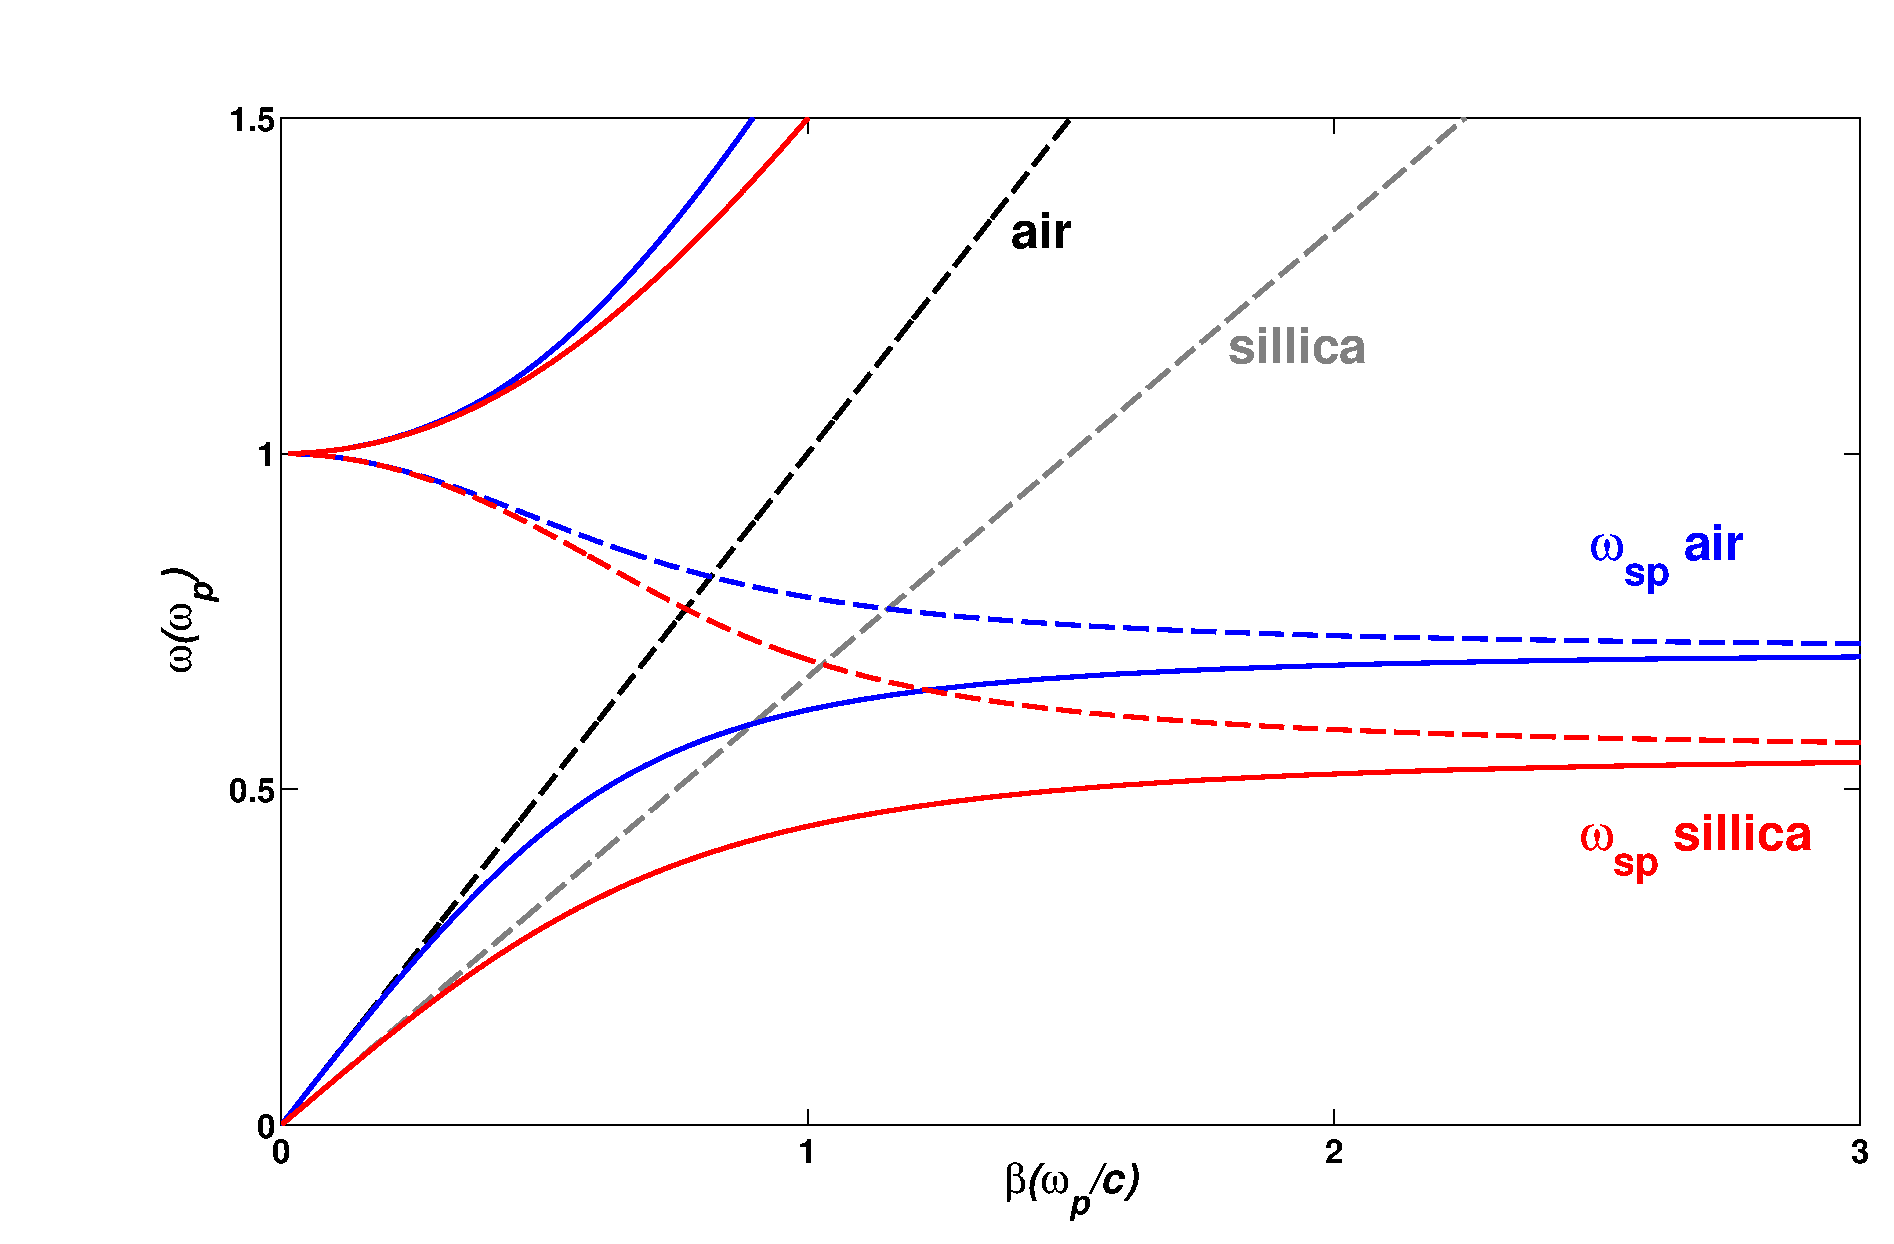
\includegraphics[scale=0.4]{THM/SPPdisp.eps}
\caption{\label{fig:SPPdisp}Dispersion relation of SPPs at the interface between a Drude metal with negligible collision frequency and air (blue curves) and silica (red curves).}
\end{figure}
For small wave vectors SPPs propagation constant $\beta$ is close to $k_0$ at the light line, in the opposite regime of the frequency close to surface plasmon frequency $\omega_p$. It also shows that the SPPs line lying to the right of the respective light lines of air and silica, so that SPPs are directed by light due to phase mismatching. The wave vector mismatch between SPPs and radiation modes needs to be overcome in order to excite or detect SPPs. This can be achieved by multiple methods~\cite{raether1988surface}. In the Otto configuration, light in a prism that is brought in close vicinity to a metal surface can excite SPPs through coupling to the evanescent field. Because light in the prism has a larger wave vector than that in air, it can be phase-matched to the SPPs. In the related Kretschmann-Raether geometry, coupling to SPPs occurs through a metal film that is deposited on a prism. In the grating coupling configuration, metal surface with a shallow grating of grooves or holes with lattice constant $a$. For the simple 1D grating of grooves depicted in Figure~\ref{fig:grating},
\begin{figure}[htb]
\centering
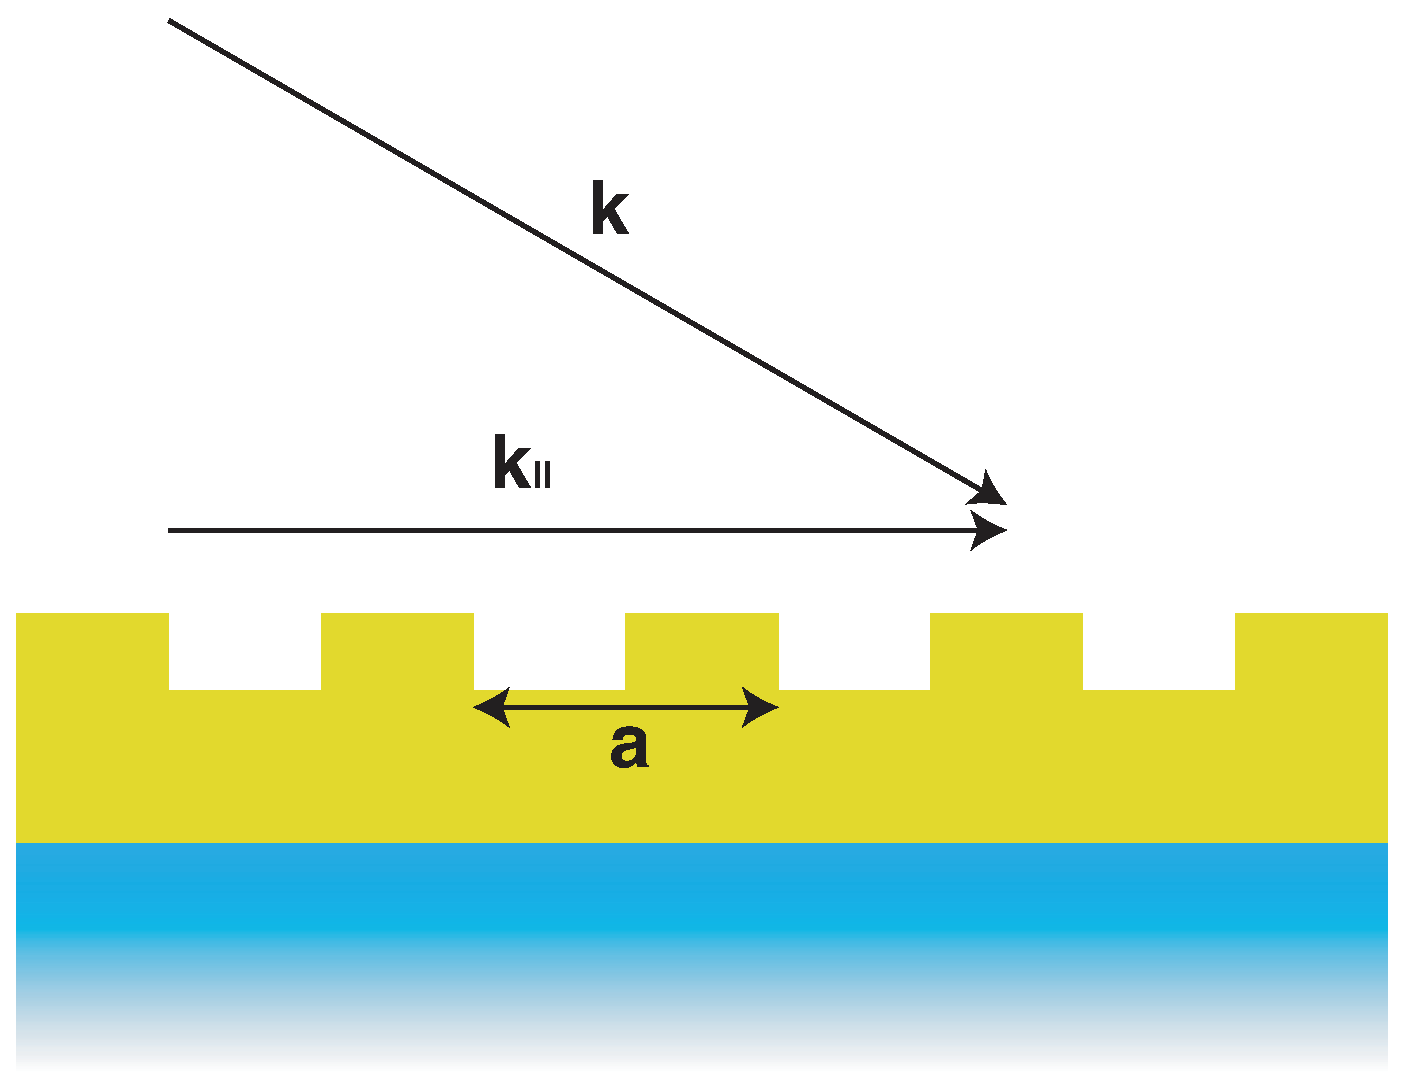
\includegraphics[scale=0.5]{THM/grating.eps}
\caption{\label{fig:grating}Phase-matching of light to SPPs the grating coupling configuration.}
\end{figure}
phase-matching takes place when the condition is fulfilled
\begin{equation}
\beta = k_0 \sin{\theta} \pm \nu g\text{,}
\end{equation}
where $g=\frac{2\pi}{a}$ is the reciprocal vector of the grating, and $\nu=(1,2,3\dots)$.
As with prism coupling, excitation of SPPs is detected as a minimum in the reflected light. The reverse process can also take place, SPPs propagating along a surface modulated with a grating can couple to light and thus radiate. 

%\bibliographystyle{unsrt}
%\bibliography{thesisbib}           =>  \chapter{Theory of surface plasmon polaritons in metallic nano-structures}
\label{c:thm}
\section{Definition of plasmon}

Plasmon is collective oscillation of conduction electron gas, a quasi-particle resulting from the quantization of plasma oscillations just like phonons are quantizations of mechanical vibrations. The simplest case is the volume plasmon as shown in Figure~\ref{fig:bulk}.
\begin{figure}[htb]
\centering
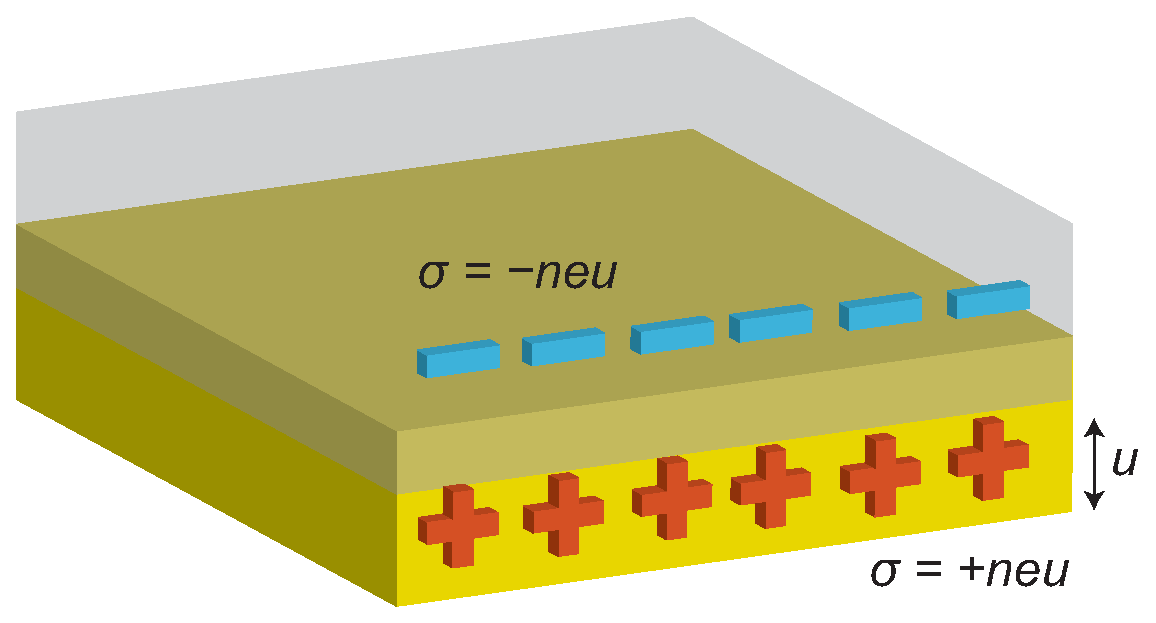
\includegraphics[scale=0.5]{THM/bulk.eps}
\caption{\label{fig:bulk}Longitudinal collective oscillations of the conduction electrons of a metal (Volume plasmons)}
\end{figure}
 We can derive plasma frequency $\omega_p$ from the simple harmonics oscillation model, a collective displacement of the electron cloud by a distance $u$ leads to a surface charge density $\sigma = \pm neu$ at the slab boundaries. This establishes a homogeneous electric field $\mathbf{E} = \frac{neu}{\varepsilon_0}$ inside the slab. Thus, the displaced electrons experience a restoring force, and their movement can be described by the equation of motion $nm\ddot{u} = -ne\mathbf{E}$. Inserting the expression for the electric field, this leads to
 \begin{subequations}
 \begin{align}
 nm\ddot{u} = -\frac{n^2e^2u}{\varepsilon_0} \\
 \ddot{u} + {\omega_p}^{2}u = 0\text{.}
 \end{align}
 \end{subequations}
  The plasma frequency $\omega_p = \sqrt{\frac{ne^2}{\varepsilon_0m}}$ can thus be recognized as the natural frequency of a free oscillation of the electron sea. The quanta of these charge oscillations are called plasmons. Due to the longitudinal nature of the excitation, volume plasmons do not couple to transverse electromagnetic waves, and can only be excited by particle impact. We can derive the dispersion relation of the generalization of volume plasmons, traveling plasma waves, from curl electric field equations (Equations~\ref{eq:curlE})
 \begin{subequations}
 \begin{align}
 \curl{\curl \mathbf{E}} &= -\mu_0 \frac{\partial^2\mathbf{D}}{\partial t^2}\label{eq:curlE}\\
\mathbf{K}( \mathbf{K}\cdot \mathbf{E}-K^{ 2 }\mathbf{E} ) &=-\varepsilon ( \mathbf{K},\omega  ) \frac { { \omega  }^{ 2 } }{ { c }^{ 2 } } \mathbf{E}
 \end{align}
 \end{subequations}  
and plasma model, and a simple equation of motion for an electron of the plasma subjected to an external electric field $\mathbf{E}$
 \begin{equation}
m\ddot{\mathbf{x}} + m\gamma\dot{\mathbf{x}} = -e\mathbf{E}\text{.}
\end{equation}
Assuming a harmonic time dependence $\mathbf{E}( t )=\mathbf{E}_0\mathrm{e}^{-i\omega t}$ of the driving field, a particular solution of this equation describing the oscillation of the electron is $\mathbf{x} ( t ) = \mathbf{x}_0 \mathrm{e}^{-i\omega t} $. The complex amplitude $\mathbf{x}_0$ incorporates any phase shifts between driving field and response via
\begin{equation}
\mathbf{x} ( t ) = \frac{e}{m( \omega^2 + i\gamma\omega )}\mathbf{E}( t )\text{.}
\end{equation}
The displaced electrons contribute to the macroscopic polarization
\begin{equation}
\mathbf{P}=-\frac{ne^2}{m( \omega^2 + i\gamma\omega )}\mathbf{E}( t )\text{.}
\end{equation}
Inserting $\mathbf{P}$ into dielectric displacement field equation $\mathbf{D} = \varepsilon_0\mathbf{E} + \mathbf{P}$ yields
\begin{equation}
\mathbf{D} = \varepsilon_0(1-\frac{\omega_p^2}{\omega^2 + i\gamma\omega})\mathbf{E}\text{,}
\end{equation}
where $\omega_p^2 = \frac{ne^2}{\varepsilon_0m}$. Therefore, the dielectric function of the free electron gas
\begin{equation}
\varepsilon(\omega) = 1- \frac{\omega_p^2}{\omega^2 + i\gamma\omega}\text{.}\label{eq:dielefu}
\end{equation}
We arrive at the desired result by using equation~\ref{eq:dielefu} and the generic dispersion relation $K^2=\varepsilon(\mathbf{K},\omega)\frac{\omega^2}{c^2}$, the dispersion relation of traveling waves becomes
\begin{equation}
\omega^2 = \omega_p^2 + \mathbf{K}^2c^2\text{.}
\end{equation}
From this relation, we can figure out the oscillation properties in any frequency of external field. Note that this branch can not confine the electromagnetic waves, it would radiate out the energy, so this mode is also called radiative surface plasmon.

\section{Surface plasmon polaritons at interface between dielectric and metal}

Surface plasmon polaritons (SPPs) are eigenmodes of transverse magnetic (TM) waves, which coupling the electromagnetic fields to oscillations of the conductor's electron plasma, propagate at a interface between dielectric and metal, and are confined in perpendicular direction. Providing a flat interface between dielectric and metal half-spaces with dielectric constants $\varepsilon_d$ and $\varepsilon_m$ , respectively, and assuming the interface normal to z direction and the SPPs propagate along the $x$ direction, the SPP wave vector $\beta$ is related to the frequency $\omega$ through the dispersion relation
\begin{equation}
\beta = k_0\sqrt{\frac{\varepsilon_d\varepsilon_m}{\varepsilon_d + \varepsilon_m}}\text{,}\label{eq:sppsdisp}
\end{equation}
where $k_0 = \omega/c$ is the free-space wave vector. We take $\omega$ to be real and allow $\beta$ to be complex.

The optical response of metals is often described by the Drude model for a free-electron gas~\cite{kittel1976introduction},
\begin{equation}
\varepsilon_{Drude}(\omega)=1-\frac{\omega_p^2}{\omega^2+i\Gamma\omega}\text{,}
\end{equation}
in which $\Gamma$ is a damping rate due to electron-electron and electron-phonon scattering.
Figure~\ref{fig:SPPdisp} shows the dispersion curve~\ref{eq:sppsdisp} with Drude metal  in the absence of losses ($\Gamma=0$) for air ($\varepsilon_d = 1$) and fused silica ($\varepsilon_d = 2.25$) interface.
\begin{figure}[htb]
\centering
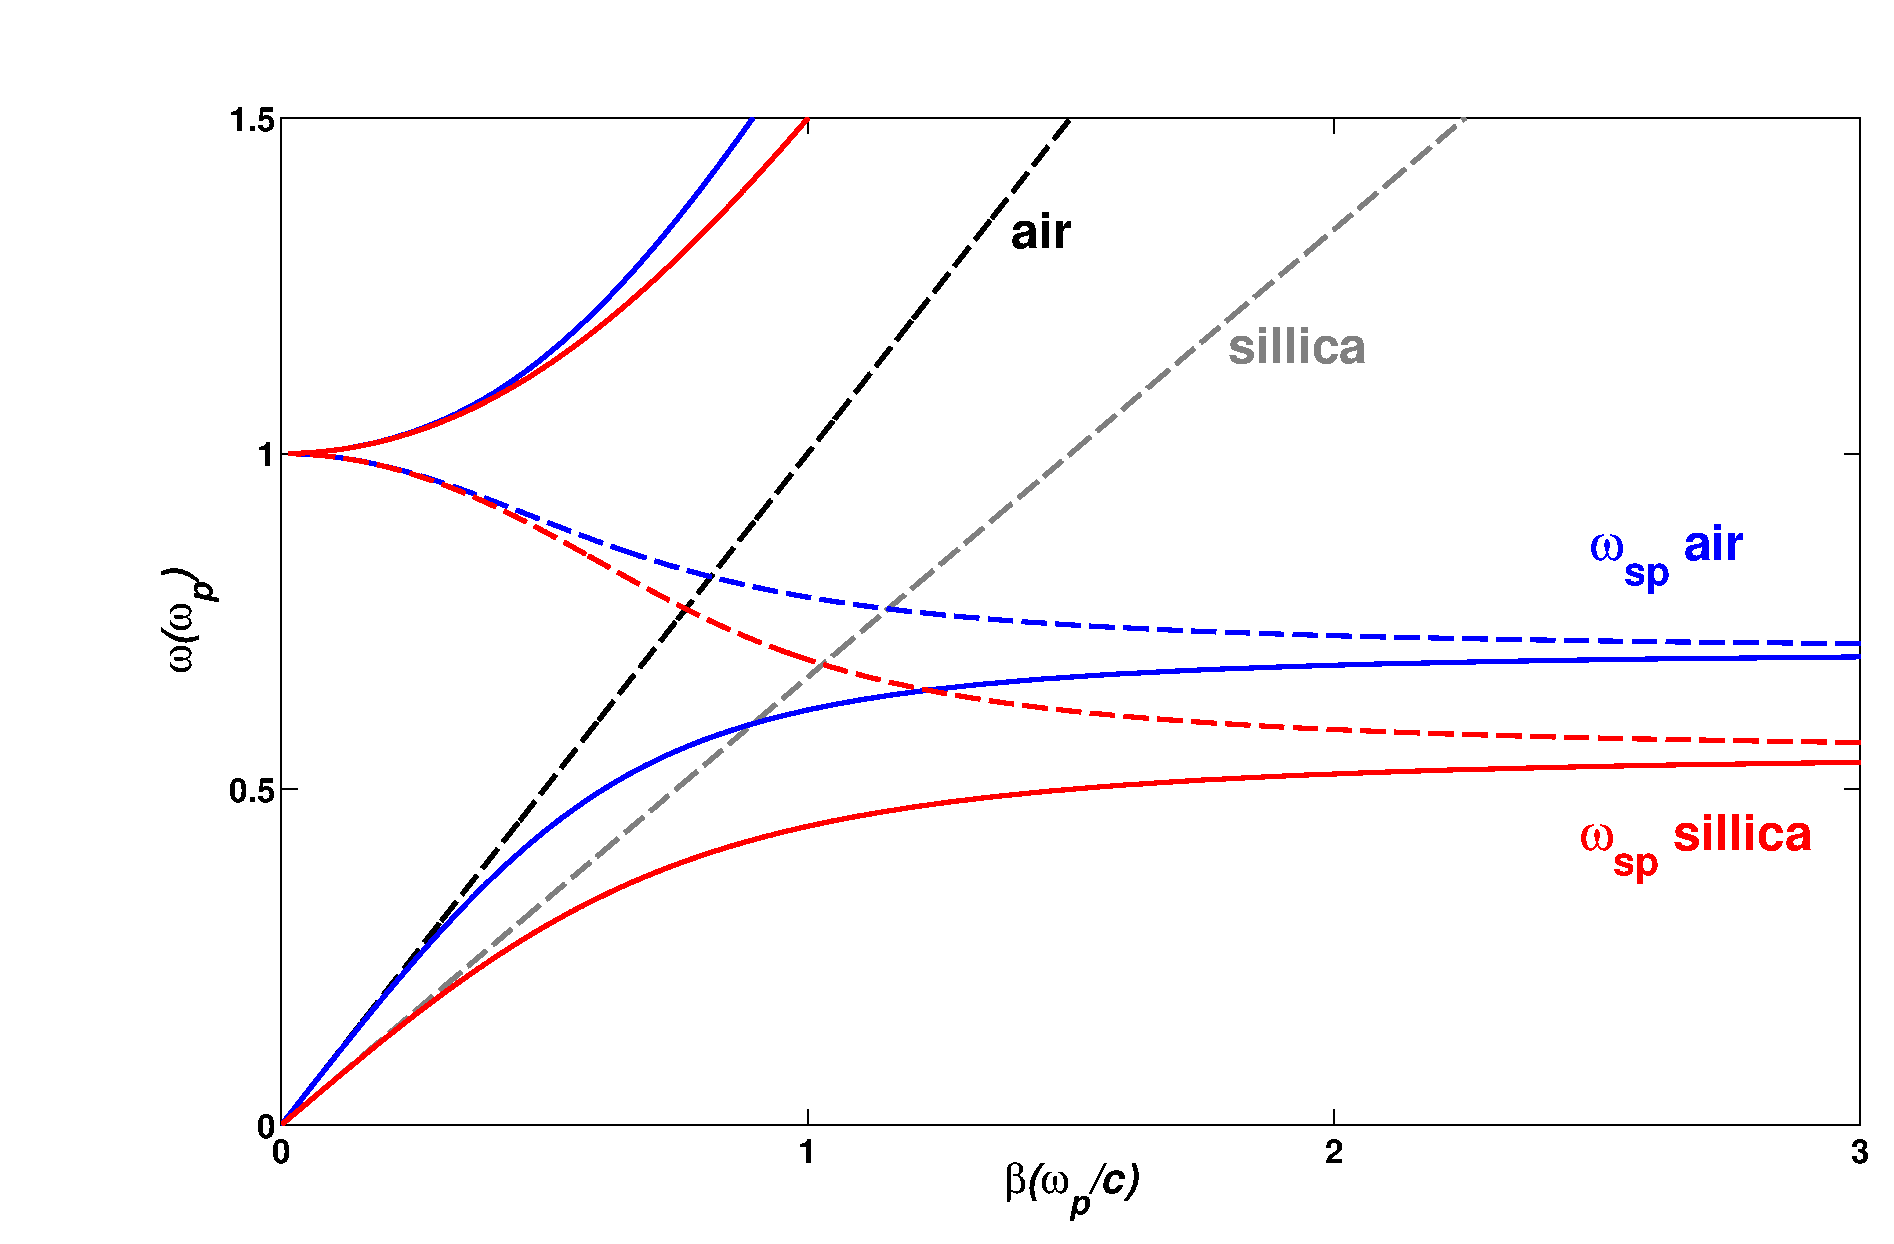
\includegraphics[scale=0.4]{THM/SPPdisp.eps}
\caption{\label{fig:SPPdisp}Dispersion relation of SPPs at the interface between a Drude metal with negligible collision frequency and air (blue curves) and silica (red curves).}
\end{figure}
For small wave vectors SPPs propagation constant $\beta$ is close to $k_0$ at the light line, in the opposite regime of the frequency close to surface plasmon frequency $\omega_p$. It also shows that the SPPs line lying to the right of the respective light lines of air and silica, so that SPPs are directed by light due to phase mismatching. The wave vector mismatch between SPPs and radiation modes needs to be overcome in order to excite or detect SPPs. This can be achieved by multiple methods~\cite{raether1988surface}. In the Otto configuration, light in a prism that is brought in close vicinity to a metal surface can excite SPPs through coupling to the evanescent field. Because light in the prism has a larger wave vector than that in air, it can be phase-matched to the SPPs. In the related Kretschmann-Raether geometry, coupling to SPPs occurs through a metal film that is deposited on a prism. In the grating coupling configuration, metal surface with a shallow grating of grooves or holes with lattice constant $a$. For the simple 1D grating of grooves depicted in Figure~\ref{fig:grating},
\begin{figure}[htb]
\centering
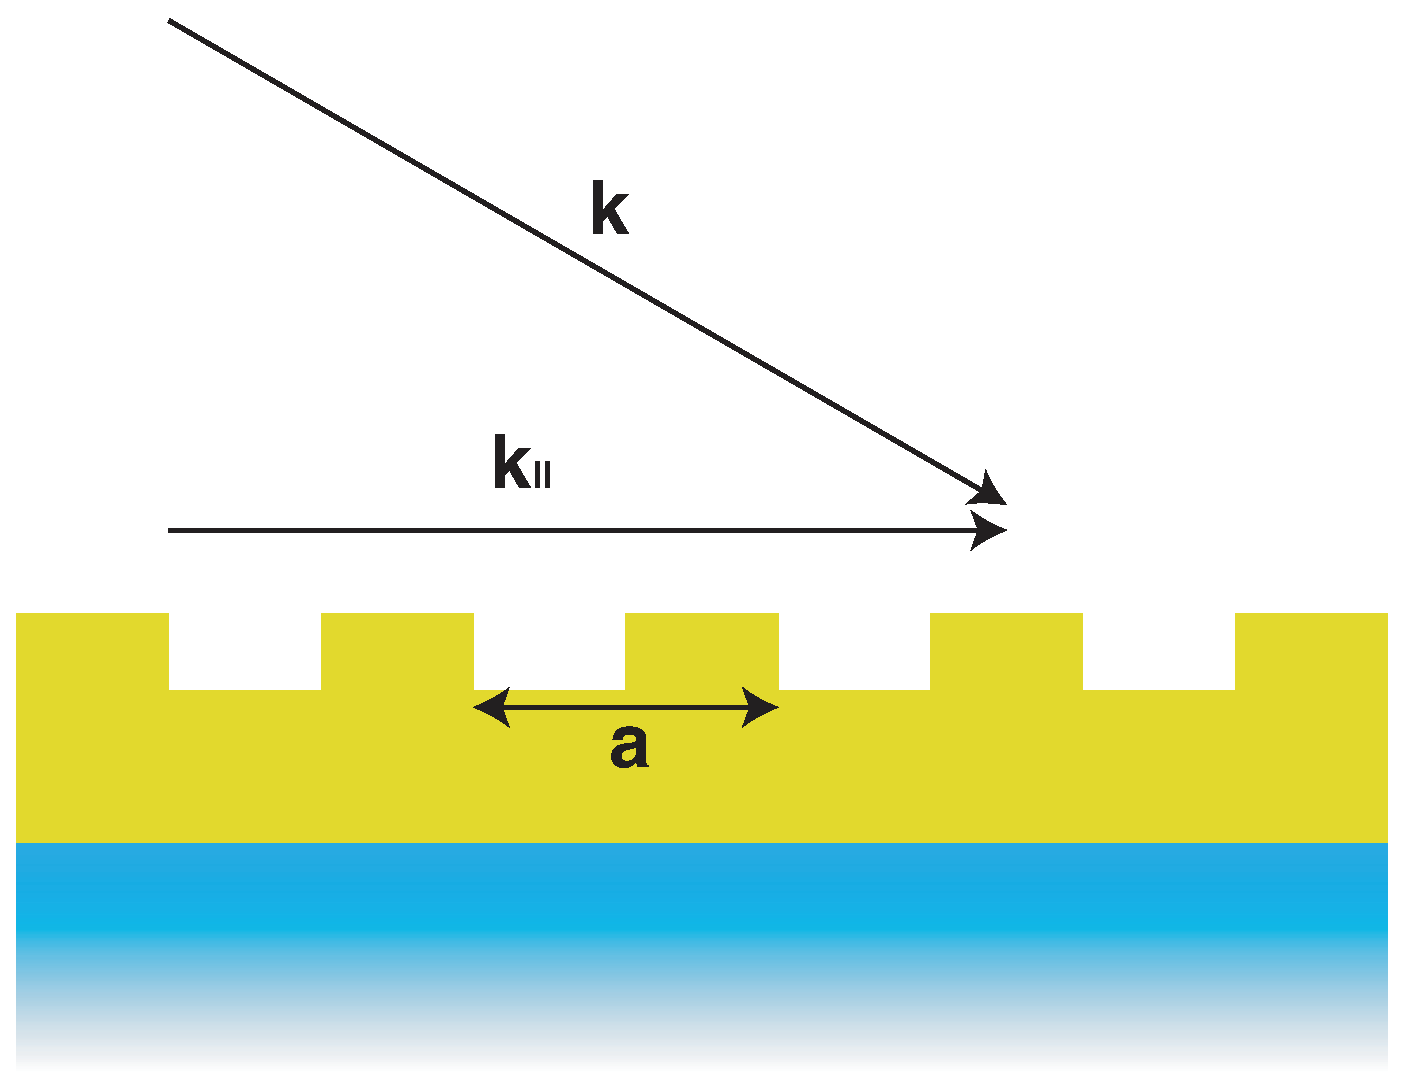
\includegraphics[scale=0.5]{THM/grating.eps}
\caption{\label{fig:grating}Phase-matching of light to SPPs the grating coupling configuration.}
\end{figure}
phase-matching takes place when the condition is fulfilled
\begin{equation}
\beta = k_0 \sin{\theta} \pm \nu g\text{,}
\end{equation}
where $g=\frac{2\pi}{a}$ is the reciprocal vector of the grating, and $\nu=(1,2,3\dots)$.
As with prism coupling, excitation of SPPs is detected as a minimum in the reflected light. The reverse process can also take place, SPPs propagating along a surface modulated with a grating can couple to light and thus radiate. 

%\bibliographystyle{unsrt}
%\bibliography{thesisbib}
\chapter{Experiment}
\label{c:exp}

\section{Atomic force microscopy}

\begin{figure}[htb]
\centering
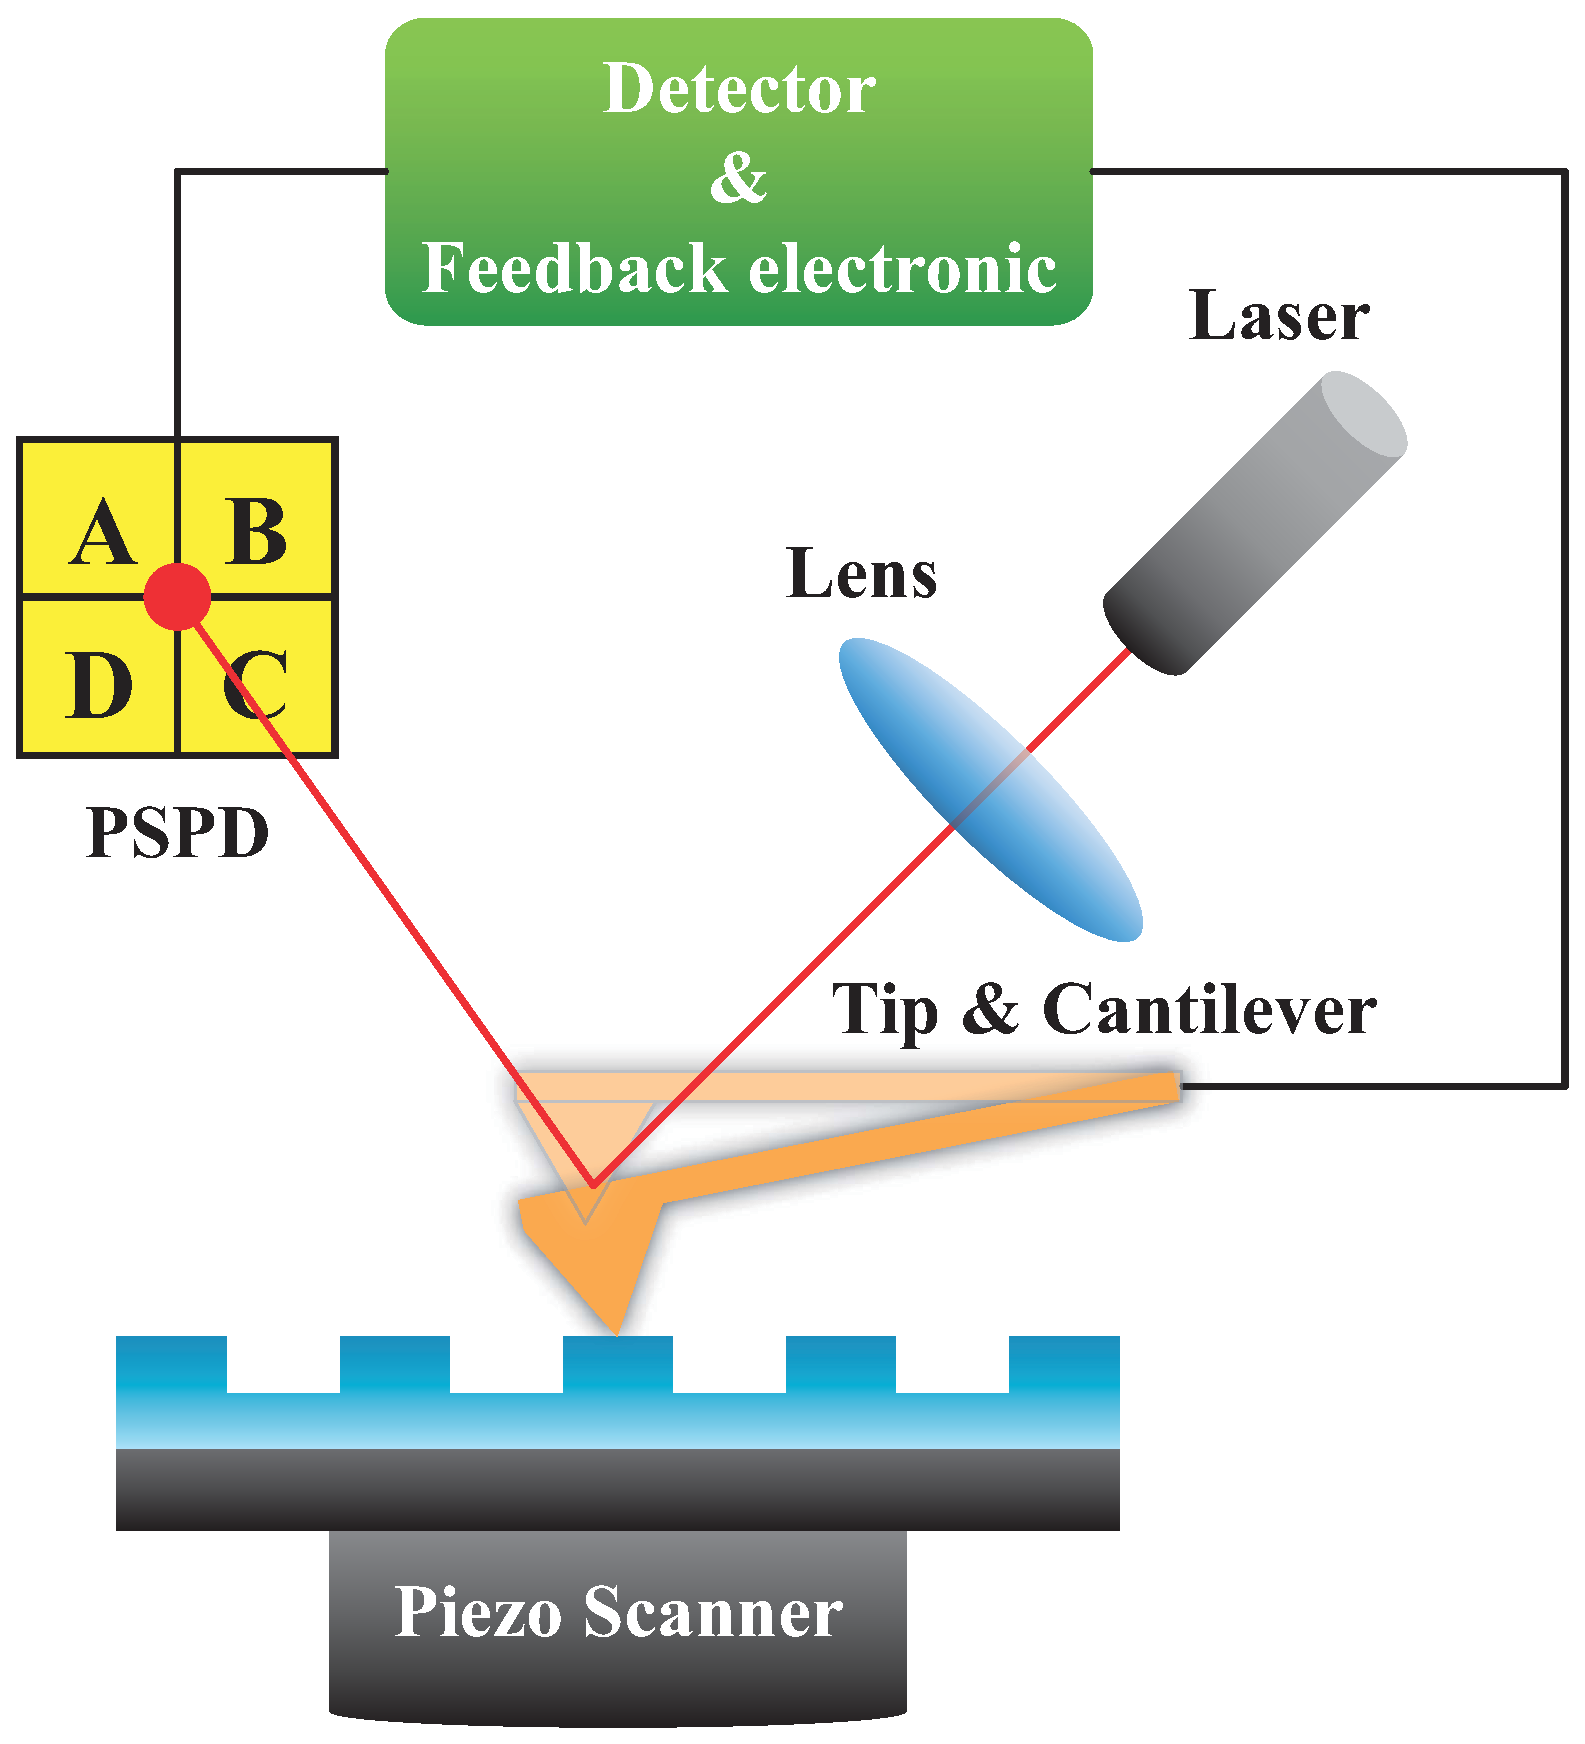
\includegraphics[scale=0.35]{EXP/afm1.eps}
\caption{\label{fig:afm1}Schematic of atomic force microscopy.}
\end{figure}
Atomic force microscope (AFM) is a type of scanning probe microscopes (SPM)~\cite{bennig1988atomic}.  The schematic of AFM is shown in Figure~\ref{fig:afm1}. AFM operates by measuring force between a probe and the specimen surfaces. In general,  the probe is a sharp tip at a cantilever's end. The cantilever can be deflected by atomic forces to sufficiently large amount, then AFM can measure the vertical and lateral deflections of the cantilever by using the optical system. A laser beam is transmitted to cantilever, and the reflected laser beam is detected with a position-sensitive photo detector (PSPD). PSPD is four-sectional that allows measuring not only vertical but lateral bending too(Figure~\ref{fig:afm2}). The output of the PSPD is provided to a computer for processing of the data for providing a topographical image of the surface with atomic resolution, and controlling the height between probe and specimen surfaces by applying voltage on piezoelectric scanner.
\begin{figure}[htb]
\centering
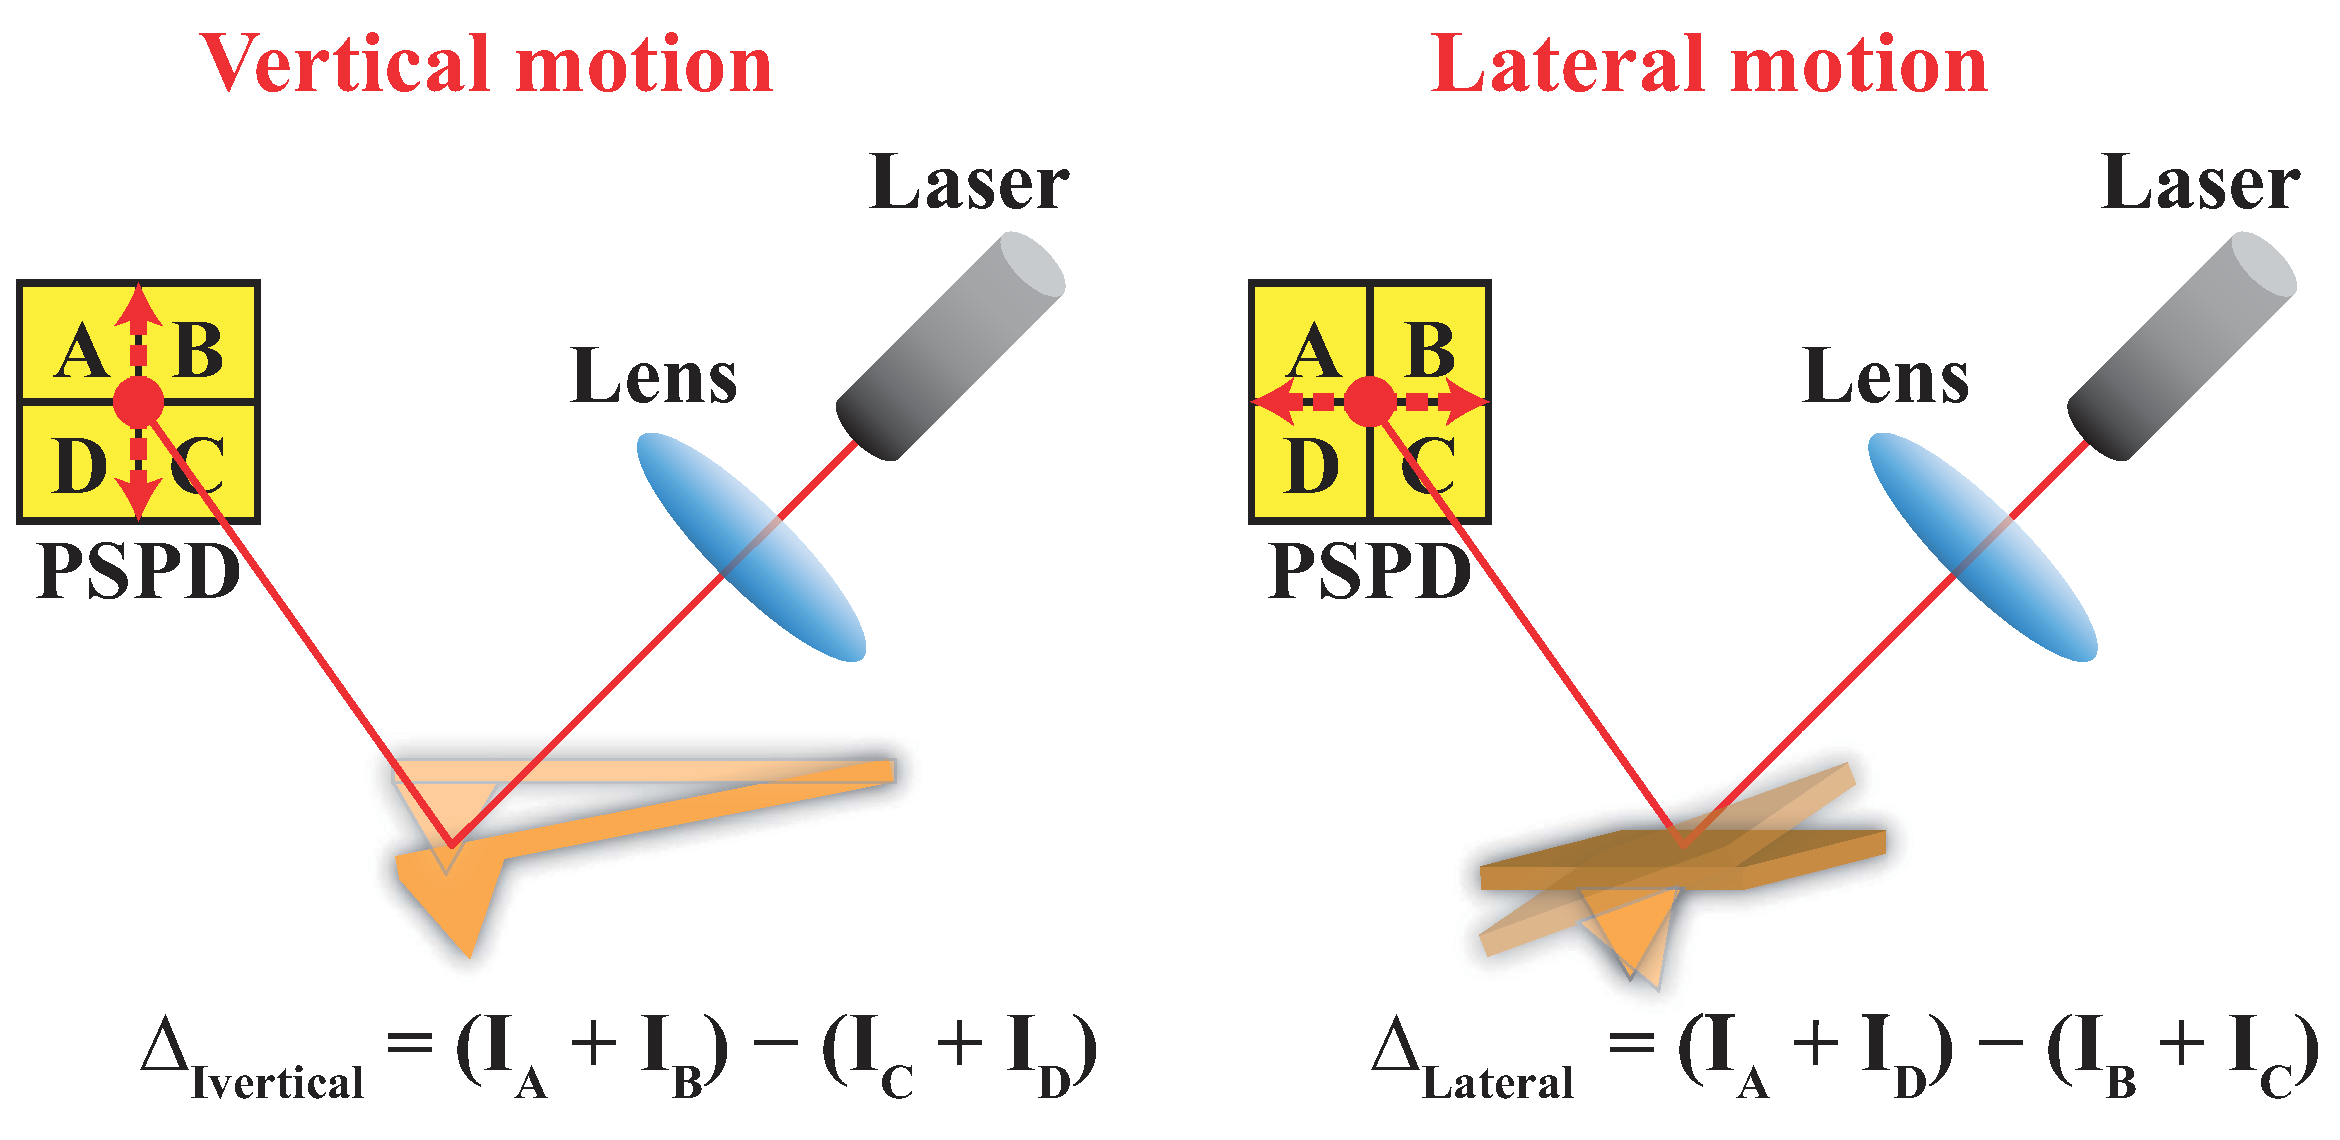
\includegraphics[scale=0.4]{EXP/afm2.eps}
\caption{\label{fig:afm2}Schematic of optical system for cantilever deflections detection.}
\end{figure}

The physical principle of the AFM operation is based on interaction between the probe tip and the specimen surface(Figure~\ref{fig:afm3}). When the cantilever approaches the specimen surface, Van der Waals forces start acting upon it . They are sufficiently far-ranging and are felt at the distance of a few tens of angstroms. Then at the distance of several angstroms repulsive force starts acting. In humid air a water layer is present on the specimen surface. The capillary force arises that holds the tip in contact with the surface and increases the minimum achievable interaction force. Electrostatic interaction between the probe and the sample may appear rather often. This can be both attraction and repulsion. Van der Waals attraction forces, capillary, electrostatic and repulsion forces at the point where the tip touches the sample and forces acting upon the tip from the deformed cantilever compensate each other in equilibrium. Based on the type and degree of this interaction the AFM modes can be broken down into contact and semi-contact(Figure~\ref{fig:afm3} ), which is a transition mode between the contact and non-contact modes.
\begin{figure}[htb]
\centering
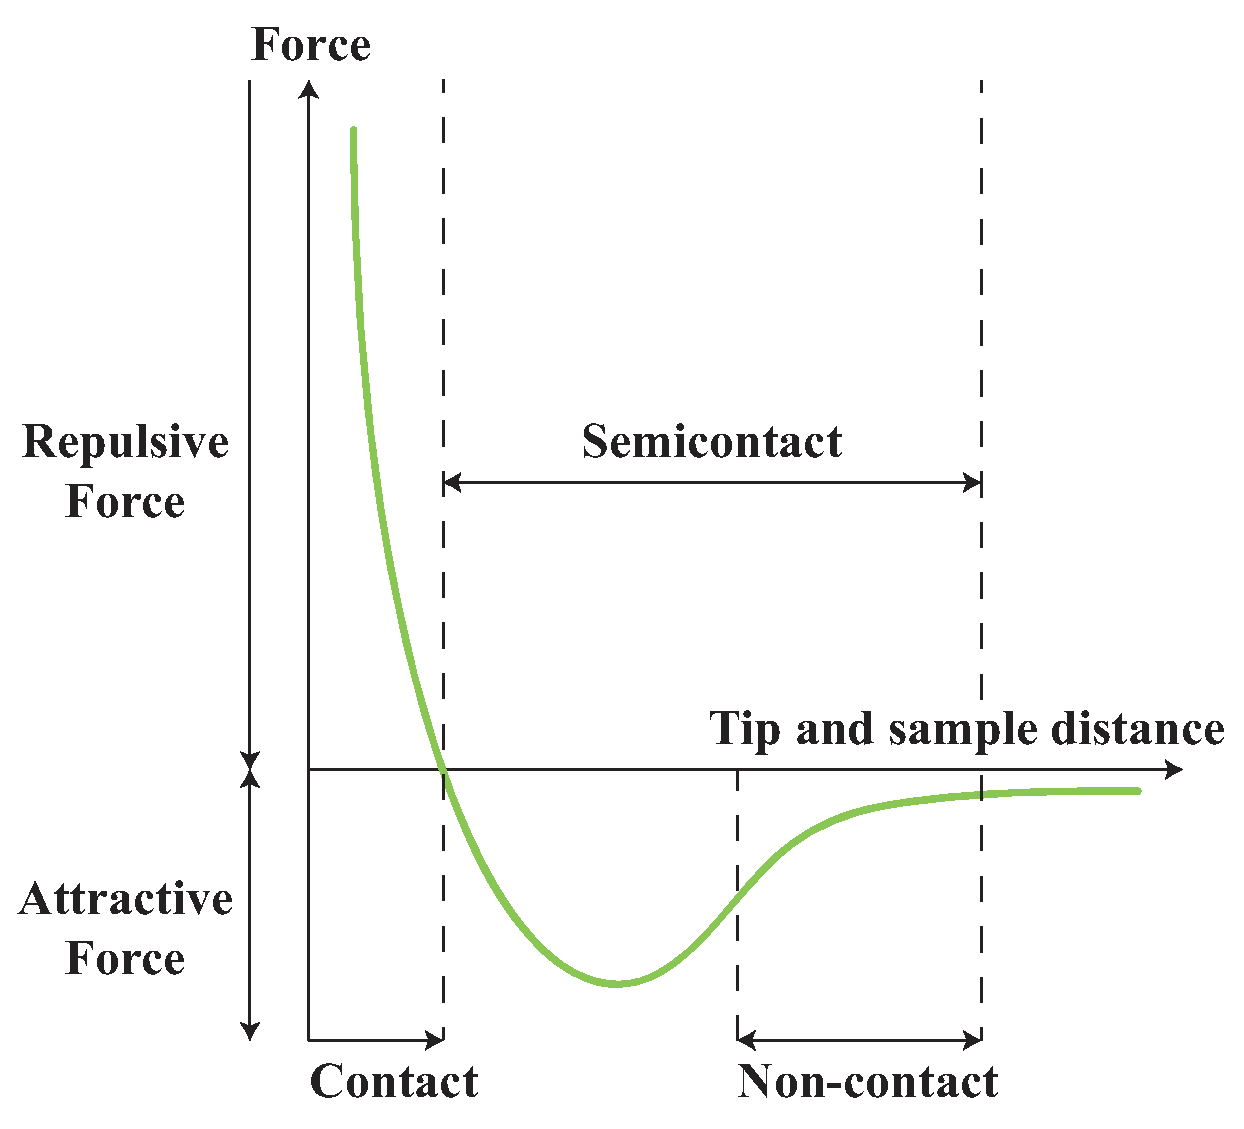
\includegraphics[scale=0.6]{EXP/afm3.eps}
\caption{\label{fig:afm3}Sketch of tip-sample forces.}
\end{figure}

\paragraph{Contact mode}

In contact mode of operation the cantilever deflection under scanning reflects repulsive force acting upon the tip. Repulsion force $\mathbf{F}$ acting upon the tip is related to the cantilever deflection value $\mathbf{x}$ under Hooke's law: $\mathbf{F}=-K \cdot  \mathbf{x}$, where $K$ is cantilever spring constant. The spring constant values for different cantilevers usually vary from 0.01 to several $\mathbf{N/m}$.

In our units the vertical cantilever deflection value is measured by means of the optical registration system and converted into electrical signal DFL (difference signal between the upper and lower halves of the PSPD) . In contact mode the DFL signal is used as a parameter characterizing the interaction force between the tip and the surface. There is a linear relationship between the DFL value and the force. In constant force mode of operation the deflection of the cantilever is maintained by the feedback circuitry on the preset value. So vertical displacement of the scanner under scanning reflects topography of sample under investigation.

Contact force microscopy is surface topography measurement in the contact mode.The microscope operation in the mode of maintaining constant interaction force between the tip and the surface sample, and is the base for measuring surface topography as well as for measuring local rigidity, local viscosity and local friction force. Constant force mode has some advantages and disadvantages. Main advantage of constant force mode is possible to measure with high resolution simultaneously with topography and some other characteristics, such as friction forces, spreading resistance etc. Constant force mode has also some disadvantages. Speed of scanning is restricted by the response time of feedback system. When exploring soft samples they can be destroyed by the scratching because the probe scanning tip is in direct contact with the surface. Therefore, under scanning soft unhomogeneous samples the local flexure of sample surface varies. As a result acquired topography of the sample can be proved distorted. Possible existence of substantial capillary forces imposed by a liquid adsorption layer can decrease the resolution.

\paragraph{Semi-contact mode}

The semi-contac mode can be characterized by some advantages in comparison with contact mode. First of all, in this mode the force of pressure of the cantilever onto the surface is less, that allows to work with softer materials such as polymers and bio-organics. The semi contact mode is also more sensitive to the interaction with the surface that gives a possibility to investigate some characteristics of the surface distribution of magnetic and electric domains, elasticity and viscosity of the surface. 

Widely used semi-contact mode has some disadvantage concerned with the usage of the feedback circuit. The scanning speed in semi-contact mode is restricted by the feedback circuit reaction time. This disadvantage can be overcome by the fact that under scanning new value of cantilever oscillation amplitude (and error signal) usually is achieved faster than preset value of the cantilever oscillation amplitude can be reached by the feedback system. Time of the reaching new value of the oscillation amplitude is determined by the oscillation period and Q-quality of the cantilever.
The feedback error signal, emerging when scanning in the semi-contact mode, contains some additional information about the topography. It can be utilized for achieving a more precise recovery of the relief. 

Additionally, similarly to the contact error mode, which can be considered as intermediate between the constant force mode and constant height mode, the feedback gain factor (i.e. the feedback processing speed) can be adjusted for the system to be able to trace subtle changes of the relief and to be too slow to trace the steep changes. Then, when the probe travels over minor irregularities, scanning will be carried out with an almost constant piezo scanner length. As a result, the slow changes of the relief will hardly show up on the images, and the steep changes will appear in high contrast. This may be helpful in finding minor irregularities on large areas against major sloping relief features. It must be noted that height of the minor irregularities must be less than amplitude of cantilever oscillation.

\section{Scanning electron microscopy}

The scanning electron microscope (SEM) is used for the observation of specimen surfaces~\cite{von1938elektronen}. When the specimen is irradiated with a fine electron beam, secondary electrons are emitted from the specimen surface. Topography of the surface can be observed by two-dimensional scanning of the electron probe over the surface and acquisition of an image from the detected secondary electrons. The concept schematic of commercial SEM (JEOL, JSM-6500F) is shown in Figure~\ref{fig:sem1}. The basic unit is composed of an electron optical system, a specimen stage, a secondary-electron detector, an image display unit, and an operation system. The electron optical system consists of an electron gun, a condenser lens and an objective lens to produce an electron probe, a scanning coil to scan the electron probe, and other components. The system inside of the microscope column are kept at vacuum.
\begin{figure}[htb]
\centering
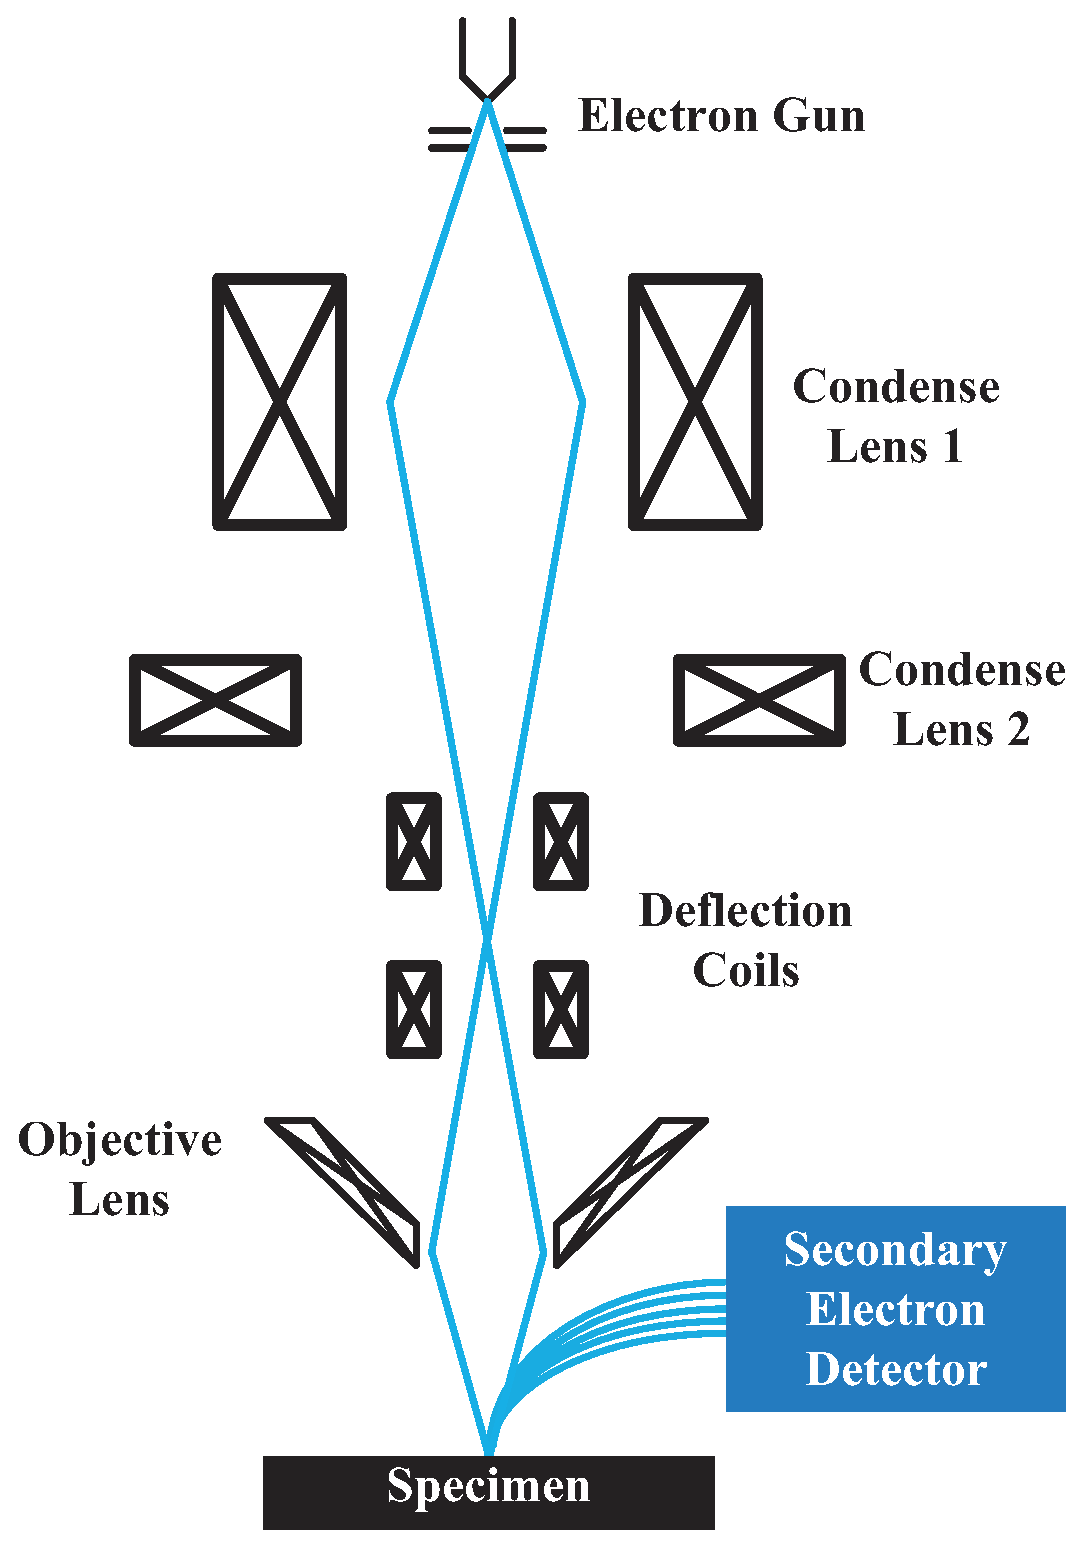
\includegraphics[scale=0.5]{EXP/SEM.eps}
\caption{\label{fig:sem1}Basic construction of a scanning electron microscopy.}
\end{figure}


The JSM-6500F utilizes a Schottky type field-emission (T-FE) gun for the electron source. The T-FE gun can constantly supply the surface of the cathode with zirconium oxide by heating the surface of cathode to 1800 K. For this reason, it can easily obtain stable and high probe current (range from several pA to 100 nA) compared with the traditional thermal emission electron gun and cold field-emission gun.

The magnetic condenser and objective lens system act to control the diameter of the beam as well as to focus the beam on the specimen due to a rotationally-symmetric magnetic field is formed when we pass a direct electric current through a coilwound electric wire in the magnetic lens. A pair of deflector coils, which between the condenser and objective lens, controlled by the scan generator, which are responsible for rastering that focused beam across the specimen surface. The size of the rastering pattern is under magnification control. The beam is rastered from left to right and top to bottom. There is a one-to-one correspondence between the rastering pattern on the specimen and the rastering pattern used to produce the image on the monitor. The resolution we choose to image at will obviously affect the number of pixels per row as well as the number of rows that constitute the scanned area.

The signal is generated from the specimen, and collected by the detector and subsequently processed to generate the image. That processing takes the intensity of the signal coming from a pixel on the specimen and converts it to a grayscale value of the corresponding monitor pixel. The monitor image is a two dimensional rastered pattern of grayscale values.

With the beam focused on the specimen surface, all we need to do to change magnification is to change the size of the rastered area on the specimen. The size of the monitor raster pattern is constant. Magnification will increase if we reduce the size of the area scanned on the specimen.

%\bibliographystyle{unsrt}
%\bibliography{thesisbib}           =>  \chapter{Experiment}
\label{c:exp}

\section{Atomic force microscopy}

\begin{figure}[htb]
\centering
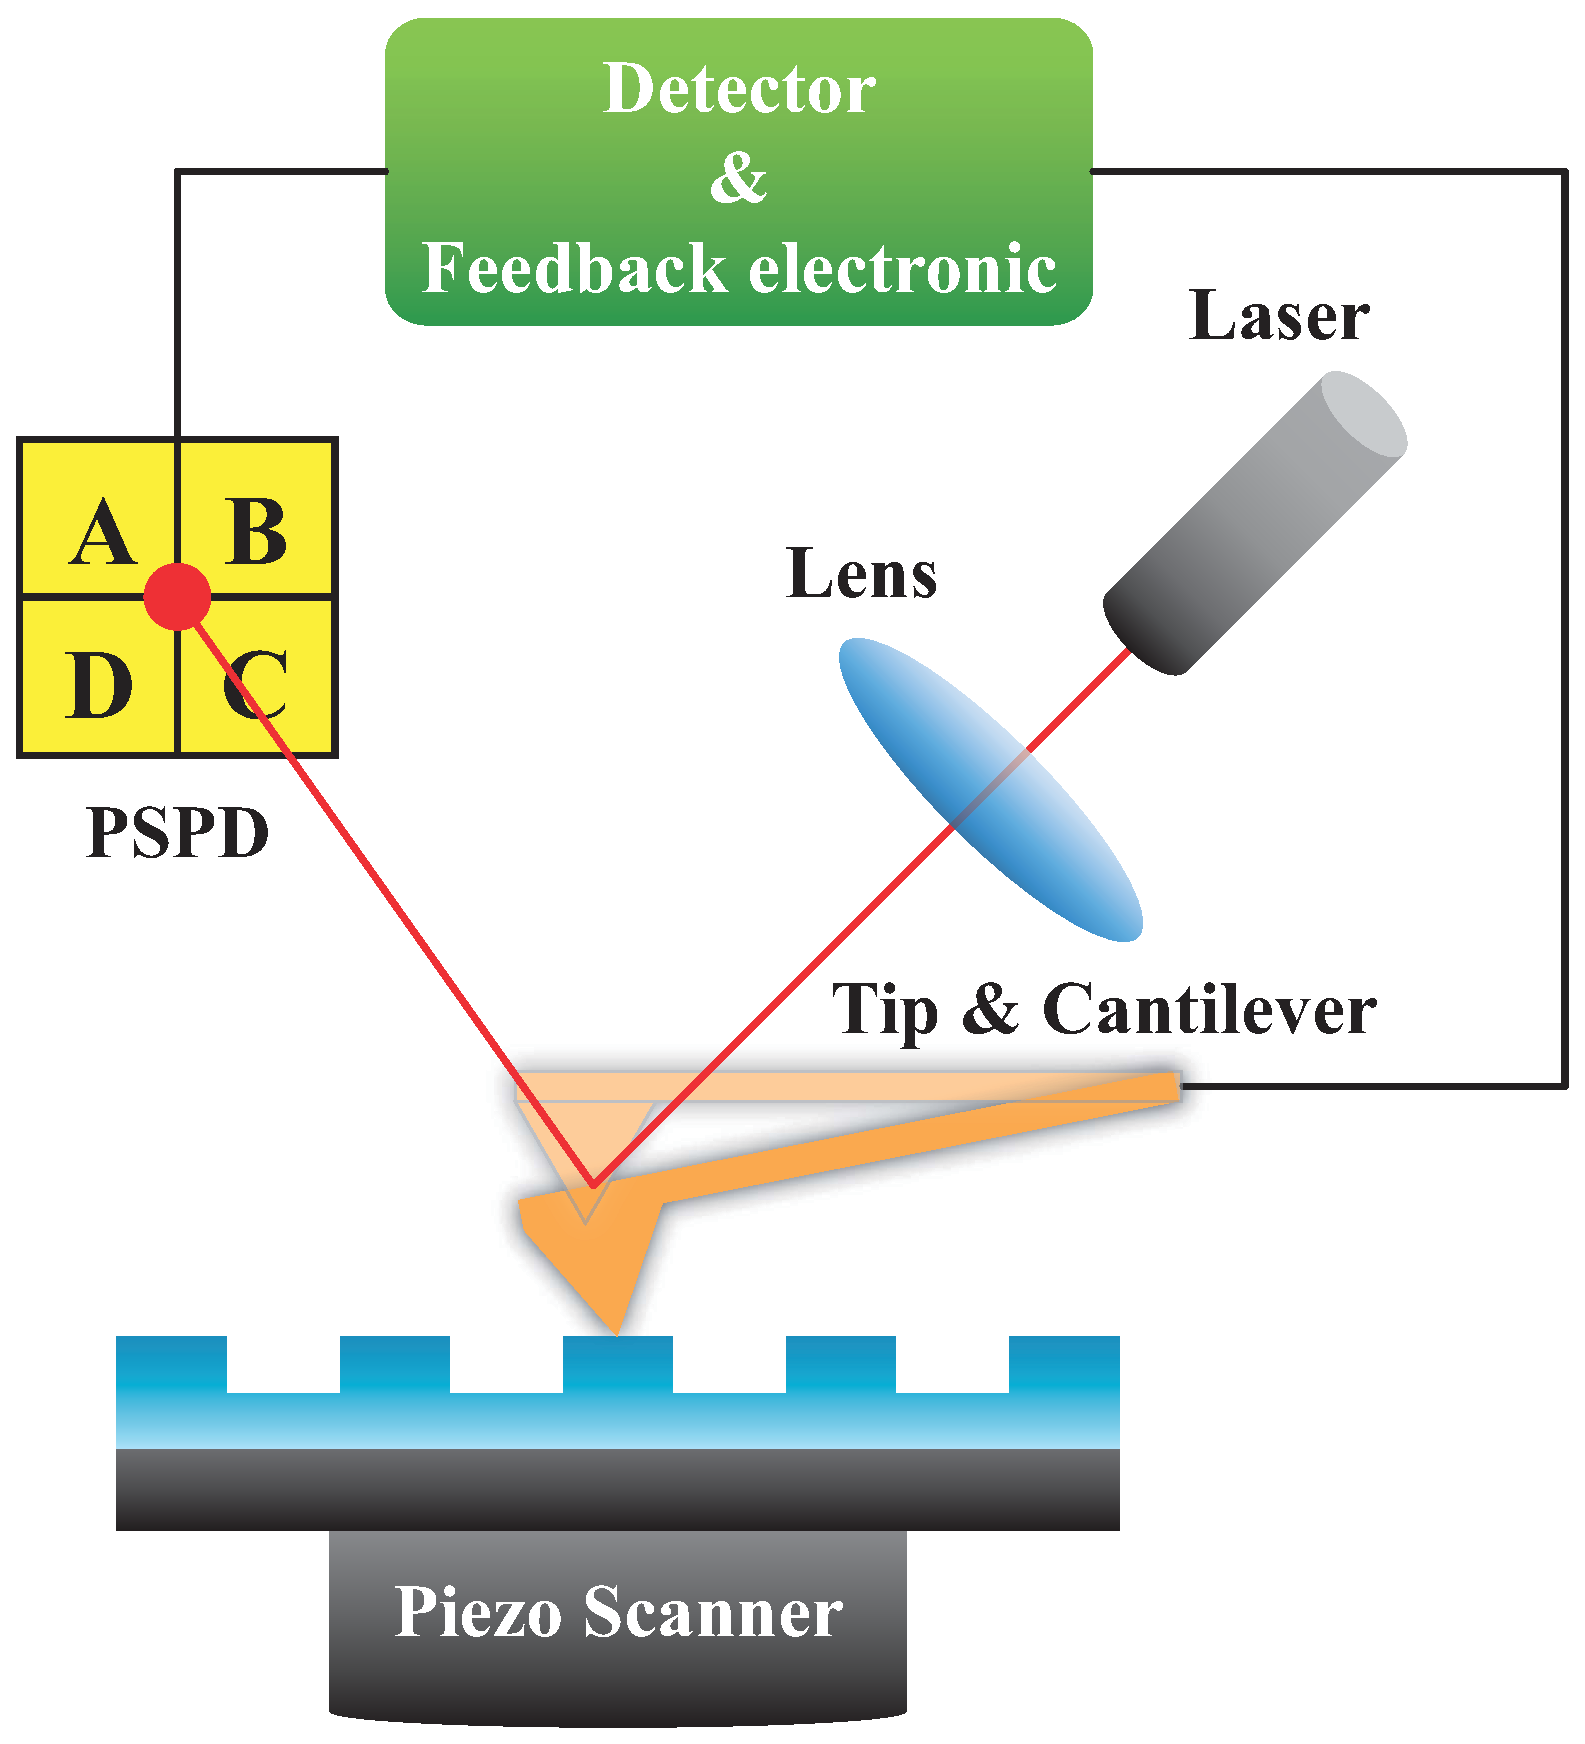
\includegraphics[scale=0.35]{EXP/afm1.eps}
\caption{\label{fig:afm1}Schematic of atomic force microscopy.}
\end{figure}
Atomic force microscope (AFM) is a type of scanning probe microscopes (SPM)~\cite{bennig1988atomic}.  The schematic of AFM is shown in Figure~\ref{fig:afm1}. AFM operates by measuring force between a probe and the specimen surfaces. In general,  the probe is a sharp tip at a cantilever's end. The cantilever can be deflected by atomic forces to sufficiently large amount, then AFM can measure the vertical and lateral deflections of the cantilever by using the optical system. A laser beam is transmitted to cantilever, and the reflected laser beam is detected with a position-sensitive photo detector (PSPD). PSPD is four-sectional that allows measuring not only vertical but lateral bending too(Figure~\ref{fig:afm2}). The output of the PSPD is provided to a computer for processing of the data for providing a topographical image of the surface with atomic resolution, and controlling the height between probe and specimen surfaces by applying voltage on piezoelectric scanner.
\begin{figure}[htb]
\centering
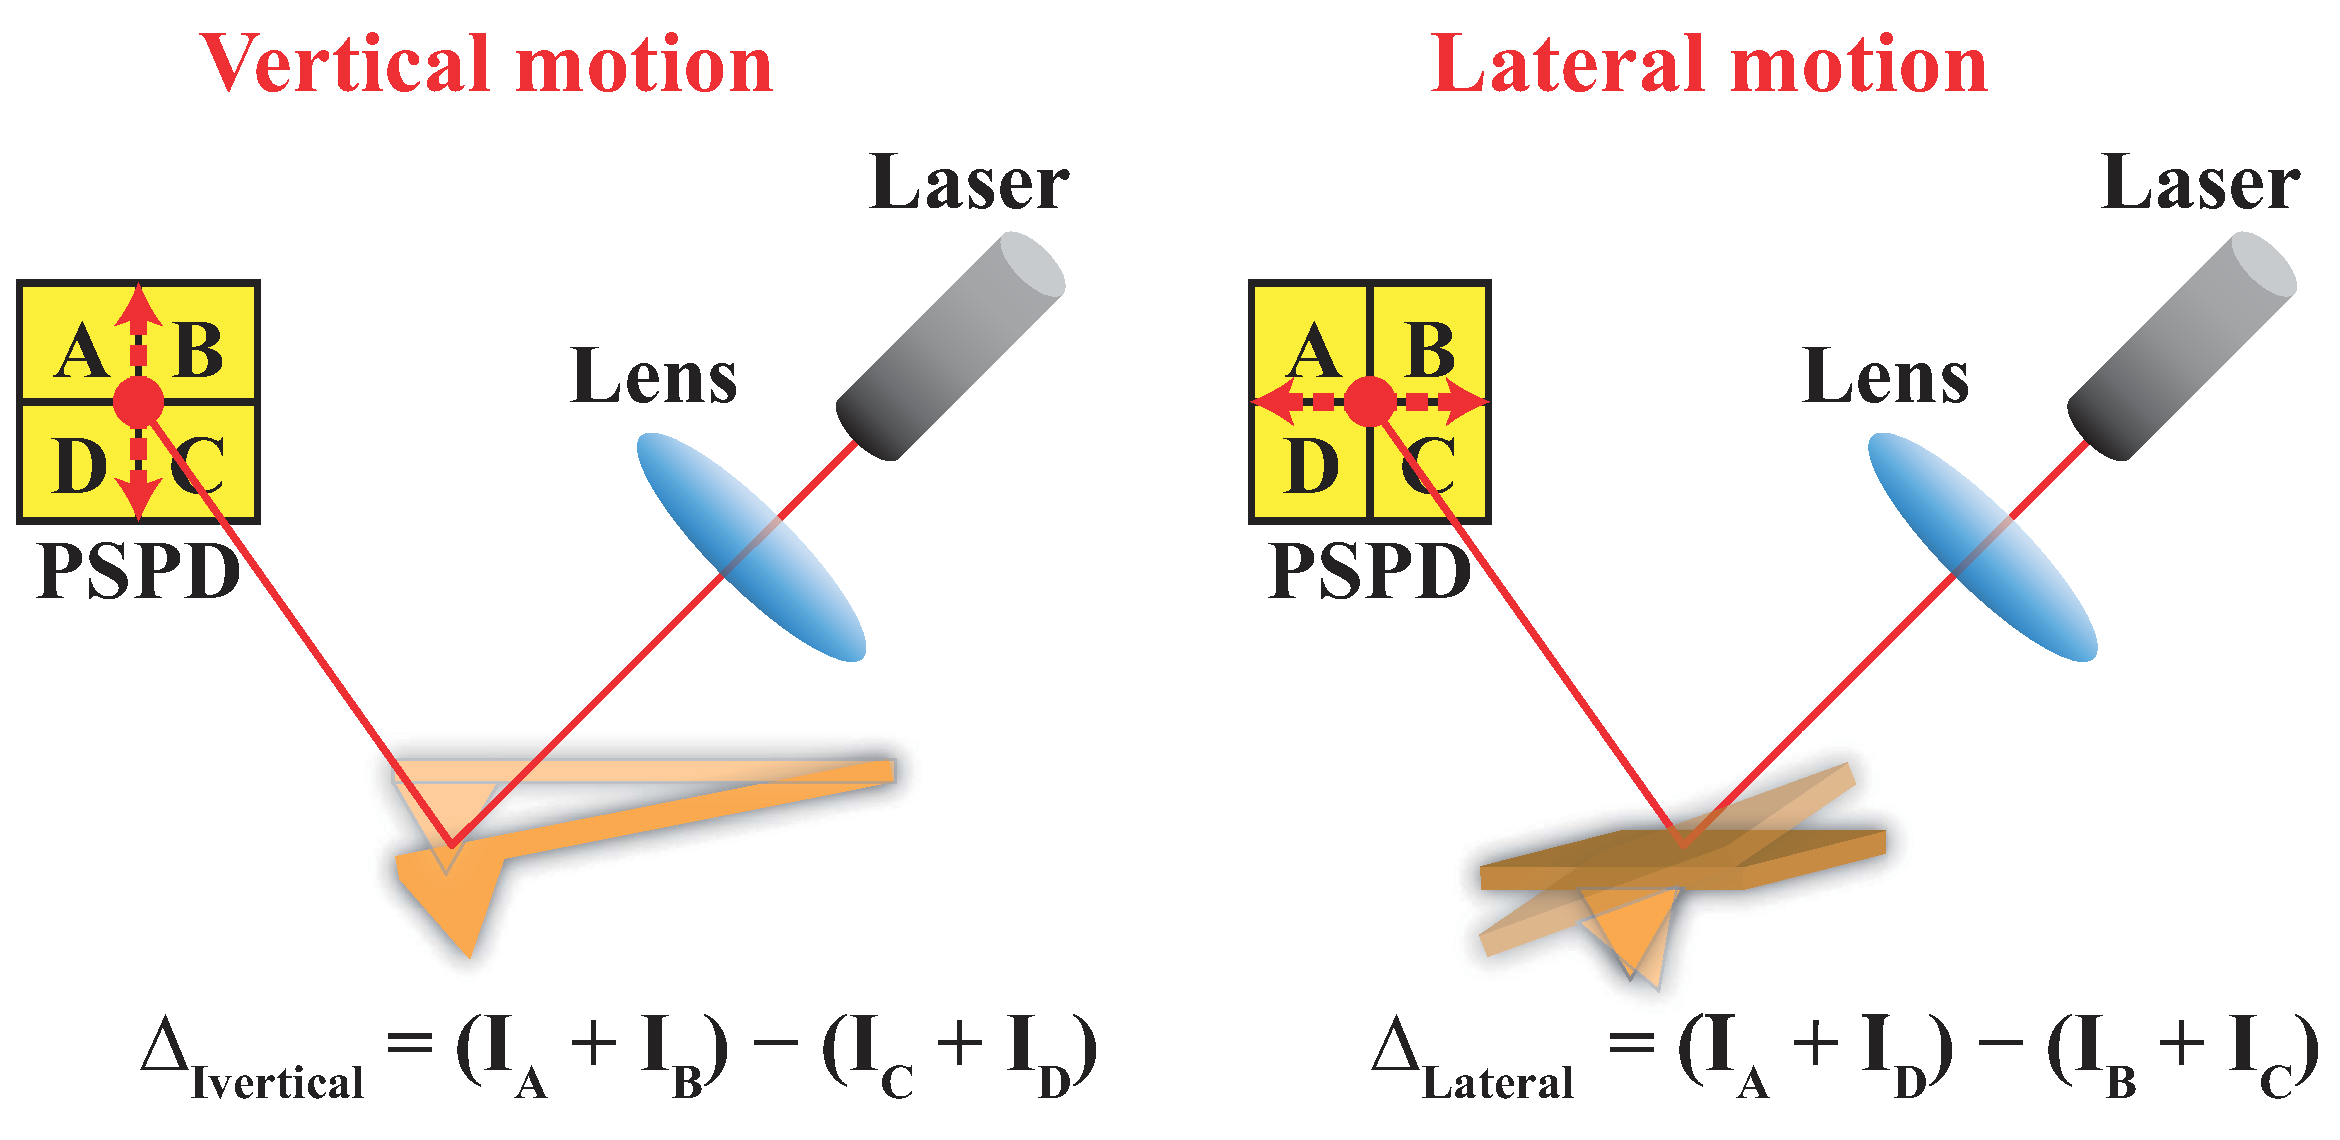
\includegraphics[scale=0.4]{EXP/afm2.eps}
\caption{\label{fig:afm2}Schematic of optical system for cantilever deflections detection.}
\end{figure}

The physical principle of the AFM operation is based on interaction between the probe tip and the specimen surface(Figure~\ref{fig:afm3}). When the cantilever approaches the specimen surface, Van der Waals forces start acting upon it . They are sufficiently far-ranging and are felt at the distance of a few tens of angstroms. Then at the distance of several angstroms repulsive force starts acting. In humid air a water layer is present on the specimen surface. The capillary force arises that holds the tip in contact with the surface and increases the minimum achievable interaction force. Electrostatic interaction between the probe and the sample may appear rather often. This can be both attraction and repulsion. Van der Waals attraction forces, capillary, electrostatic and repulsion forces at the point where the tip touches the sample and forces acting upon the tip from the deformed cantilever compensate each other in equilibrium. Based on the type and degree of this interaction the AFM modes can be broken down into contact and semi-contact(Figure~\ref{fig:afm3} ), which is a transition mode between the contact and non-contact modes.
\begin{figure}[htb]
\centering
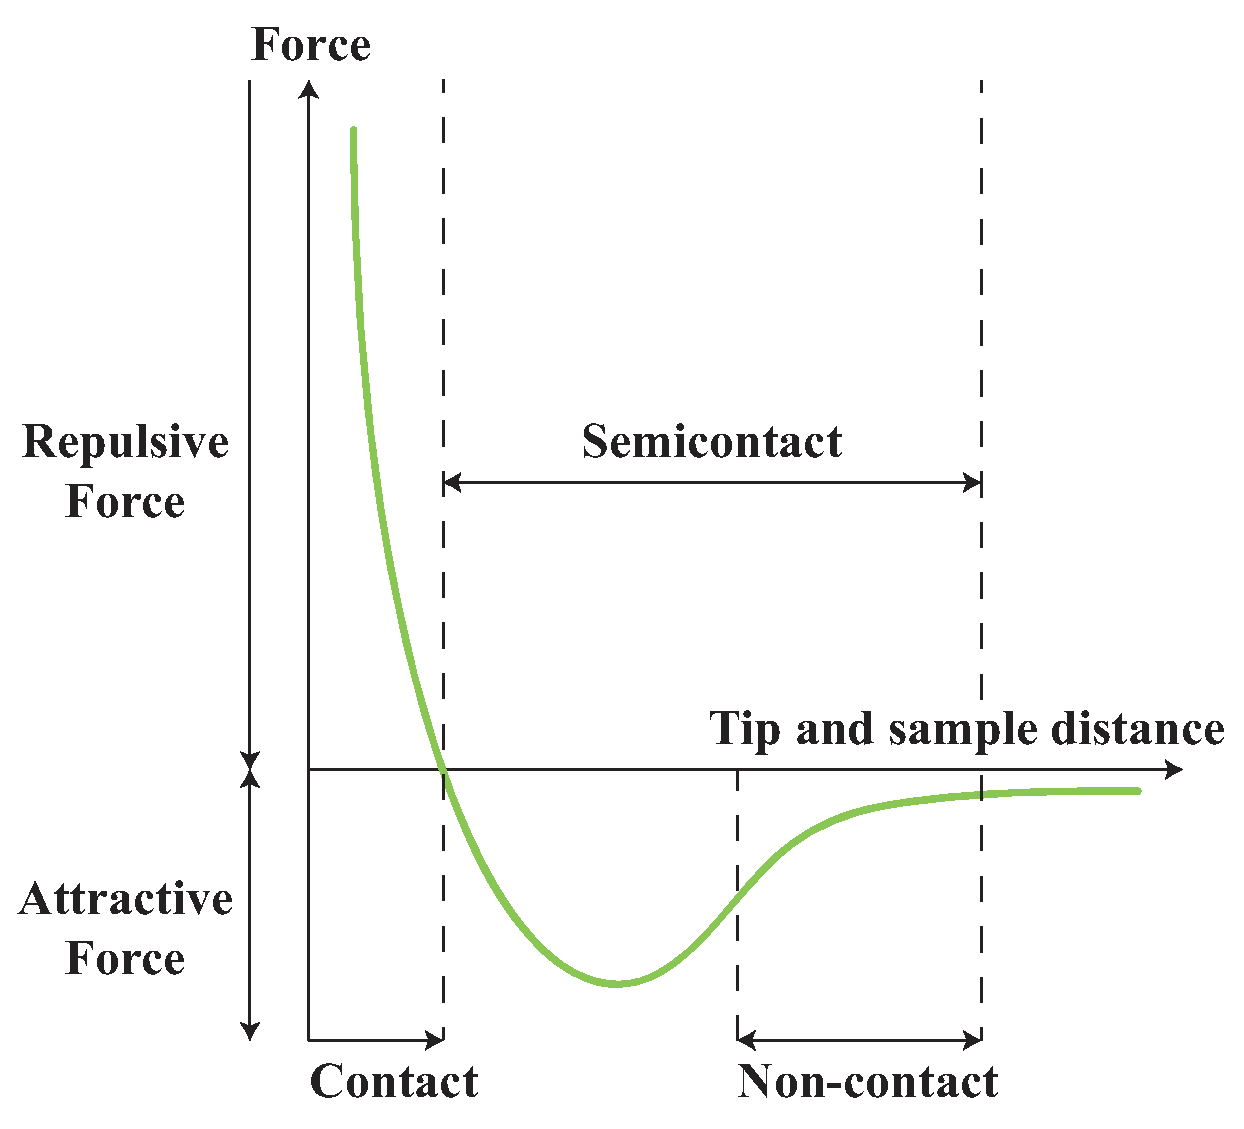
\includegraphics[scale=0.6]{EXP/afm3.eps}
\caption{\label{fig:afm3}Sketch of tip-sample forces.}
\end{figure}

\paragraph{Contact mode}

In contact mode of operation the cantilever deflection under scanning reflects repulsive force acting upon the tip. Repulsion force $\mathbf{F}$ acting upon the tip is related to the cantilever deflection value $\mathbf{x}$ under Hooke's law: $\mathbf{F}=-K \cdot  \mathbf{x}$, where $K$ is cantilever spring constant. The spring constant values for different cantilevers usually vary from 0.01 to several $\mathbf{N/m}$.

In our units the vertical cantilever deflection value is measured by means of the optical registration system and converted into electrical signal DFL (difference signal between the upper and lower halves of the PSPD) . In contact mode the DFL signal is used as a parameter characterizing the interaction force between the tip and the surface. There is a linear relationship between the DFL value and the force. In constant force mode of operation the deflection of the cantilever is maintained by the feedback circuitry on the preset value. So vertical displacement of the scanner under scanning reflects topography of sample under investigation.

Contact force microscopy is surface topography measurement in the contact mode.The microscope operation in the mode of maintaining constant interaction force between the tip and the surface sample, and is the base for measuring surface topography as well as for measuring local rigidity, local viscosity and local friction force. Constant force mode has some advantages and disadvantages. Main advantage of constant force mode is possible to measure with high resolution simultaneously with topography and some other characteristics, such as friction forces, spreading resistance etc. Constant force mode has also some disadvantages. Speed of scanning is restricted by the response time of feedback system. When exploring soft samples they can be destroyed by the scratching because the probe scanning tip is in direct contact with the surface. Therefore, under scanning soft unhomogeneous samples the local flexure of sample surface varies. As a result acquired topography of the sample can be proved distorted. Possible existence of substantial capillary forces imposed by a liquid adsorption layer can decrease the resolution.

\paragraph{Semi-contact mode}

The semi-contac mode can be characterized by some advantages in comparison with contact mode. First of all, in this mode the force of pressure of the cantilever onto the surface is less, that allows to work with softer materials such as polymers and bio-organics. The semi contact mode is also more sensitive to the interaction with the surface that gives a possibility to investigate some characteristics of the surface distribution of magnetic and electric domains, elasticity and viscosity of the surface. 

Widely used semi-contact mode has some disadvantage concerned with the usage of the feedback circuit. The scanning speed in semi-contact mode is restricted by the feedback circuit reaction time. This disadvantage can be overcome by the fact that under scanning new value of cantilever oscillation amplitude (and error signal) usually is achieved faster than preset value of the cantilever oscillation amplitude can be reached by the feedback system. Time of the reaching new value of the oscillation amplitude is determined by the oscillation period and Q-quality of the cantilever.
The feedback error signal, emerging when scanning in the semi-contact mode, contains some additional information about the topography. It can be utilized for achieving a more precise recovery of the relief. 

Additionally, similarly to the contact error mode, which can be considered as intermediate between the constant force mode and constant height mode, the feedback gain factor (i.e. the feedback processing speed) can be adjusted for the system to be able to trace subtle changes of the relief and to be too slow to trace the steep changes. Then, when the probe travels over minor irregularities, scanning will be carried out with an almost constant piezo scanner length. As a result, the slow changes of the relief will hardly show up on the images, and the steep changes will appear in high contrast. This may be helpful in finding minor irregularities on large areas against major sloping relief features. It must be noted that height of the minor irregularities must be less than amplitude of cantilever oscillation.

\section{Scanning electron microscopy}

The scanning electron microscope (SEM) is used for the observation of specimen surfaces~\cite{von1938elektronen}. When the specimen is irradiated with a fine electron beam, secondary electrons are emitted from the specimen surface. Topography of the surface can be observed by two-dimensional scanning of the electron probe over the surface and acquisition of an image from the detected secondary electrons. The concept schematic of commercial SEM (JEOL, JSM-6500F) is shown in Figure~\ref{fig:sem1}. The basic unit is composed of an electron optical system, a specimen stage, a secondary-electron detector, an image display unit, and an operation system. The electron optical system consists of an electron gun, a condenser lens and an objective lens to produce an electron probe, a scanning coil to scan the electron probe, and other components. The system inside of the microscope column are kept at vacuum.
\begin{figure}[htb]
\centering
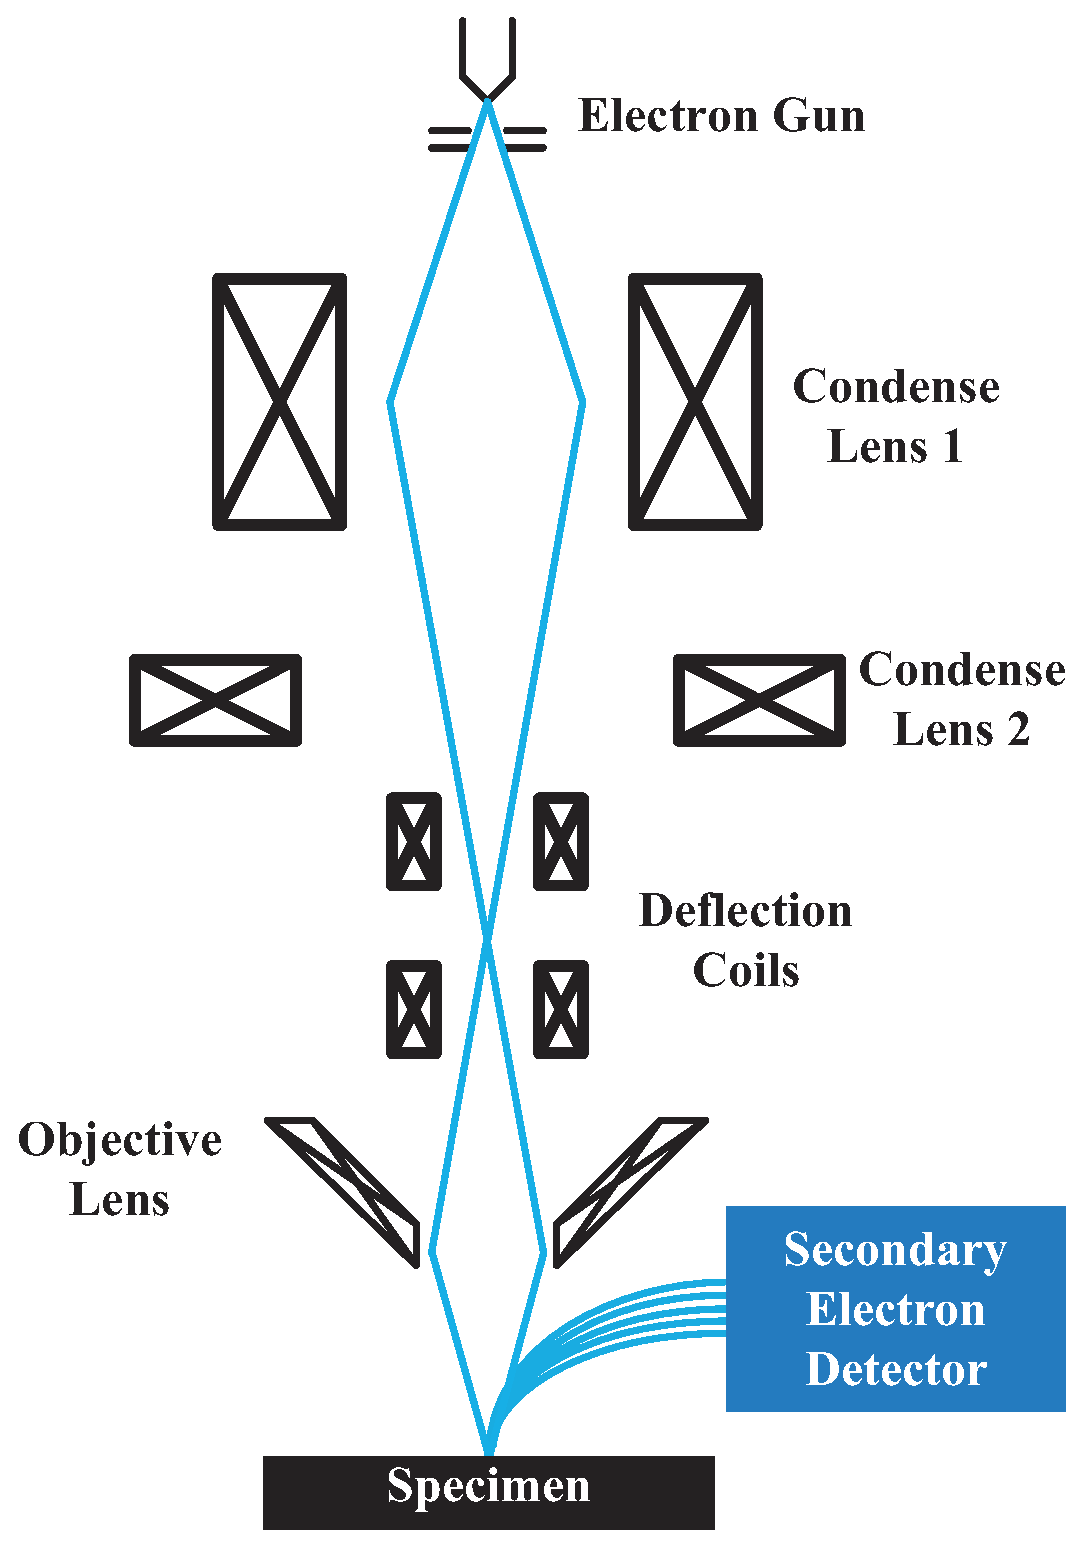
\includegraphics[scale=0.5]{EXP/SEM.eps}
\caption{\label{fig:sem1}Basic construction of a scanning electron microscopy.}
\end{figure}


The JSM-6500F utilizes a Schottky type field-emission (T-FE) gun for the electron source. The T-FE gun can constantly supply the surface of the cathode with zirconium oxide by heating the surface of cathode to 1800 K. For this reason, it can easily obtain stable and high probe current (range from several pA to 100 nA) compared with the traditional thermal emission electron gun and cold field-emission gun.

The magnetic condenser and objective lens system act to control the diameter of the beam as well as to focus the beam on the specimen due to a rotationally-symmetric magnetic field is formed when we pass a direct electric current through a coilwound electric wire in the magnetic lens. A pair of deflector coils, which between the condenser and objective lens, controlled by the scan generator, which are responsible for rastering that focused beam across the specimen surface. The size of the rastering pattern is under magnification control. The beam is rastered from left to right and top to bottom. There is a one-to-one correspondence between the rastering pattern on the specimen and the rastering pattern used to produce the image on the monitor. The resolution we choose to image at will obviously affect the number of pixels per row as well as the number of rows that constitute the scanned area.

The signal is generated from the specimen, and collected by the detector and subsequently processed to generate the image. That processing takes the intensity of the signal coming from a pixel on the specimen and converts it to a grayscale value of the corresponding monitor pixel. The monitor image is a two dimensional rastered pattern of grayscale values.

With the beam focused on the specimen surface, all we need to do to change magnification is to change the size of the rastered area on the specimen. The size of the monitor raster pattern is constant. Magnification will increase if we reduce the size of the area scanned on the specimen.

%\bibliographystyle{unsrt}
%\bibliography{thesisbib}
     \end{verbatim}
    最後記得在每個有附參考文獻的章節加上產生參考文獻的指令,即在\href{run:./introduction.tex}{introduction.tex}、\href{run:./THM.tex}{THM.tex}和\href{run:./EXP.tex}{EXP.tex}三個檔案裡最後啟動下面兩行指令
     \begin{verbatim}
%\bibliographystyle{unsrt} => \bibliographystyle{unsrt}
%\bibliography{thesisbib}  =>  \bibliography{thesisbib}
     \end{verbatim}
    而編譯時則需要對有附參考文獻的\href{run:./introduction.tex}{introduction.tex}、\href{run:./THM.tex}{THM.tex}和\href{run:./EXP.tex}{EXP.tex}各做一次BibTeX 編譯,編譯流程如下
    \begin{enumerate}[topsep=0pt, itemsep=0pt, label=\arabic{*}.]
    \item \texttt{xelatex thesis}\\ 對thesis.tex進行第一次XeLaTeX編譯,產生thesis.pdf及其他檔案
    \item \texttt{bibtex introduction}\\ 對introduction.tex進行BibTeX編譯,產生bbl檔以及blg檔
    \item \texttt{bibtex THM}\\ 對THM.tex進行BibTeX編譯,產生bbl檔以及blg檔
    \item \texttt{bibtex EXP}\\ 對EXP.tex進行BibTeX編譯,產生bbl檔以及blg檔
    \item \texttt{xelatex thesis}\\ 對thesis.tex進行第二次XeLaTeX編譯,產生目錄、圖表連結及參考文獻
    \item \texttt{xelatex thesis}\\ 對thesis.tex進行第三次XeLaTeX編譯,產生參考文獻連結,完成編譯\\
\end{enumerate} 
\item 補充說明與注意事項:
\begin{enumerate}[topsep=0pt, itemsep=0pt, label=$\bullet$]
    \item 口試委員會審定書:\\
    請到台大圖書館網頁的\href{http://etds.lib.ntu.edu.tw/etdsystem/submit/submitLogin}{電子論文服務}下載\href{http://gra103.aca.ntu.edu.tw/gra2007/gra/tienn/\%E5\%AD\%B8\%E4\%BD\%8D\%E8\%80\%83\%E8\%A9\%A6\%E8\%A1\%A8\%E5\%86\%8A/THESISSAMPLE.DOC}{論文格式範本},並修改成正確的格式,也可到此範本所在資料夾的\href{run:./cert.doc}{cert.doc}修改。當然你也可以利用LaTeX來編輯,你只要填好\href{run:./ntuvars.tex}{ntuvars.tex}檔的資料,並去除在thesis.tex裡下面這行的註解符號\texttt{\%} 
    \begin{verbatim}
%\makecertification
    \end{verbatim}
    編譯完後就可以產生審定書格式。口試通過後,請把已經簽名的審定書掃描成pdf檔,再取代原本的\href{run:./cert.pdf}{cert.pdf},即可放上已簽名的審定書。處理審定書出現的指令在thesis.tex裡 
    \begin{verbatim}
%----------- generate the certification ...
%\makecertification
%----------- includepdf by using package ...
\addcontentsline{toc}{chapter}{口試委員會審定書}
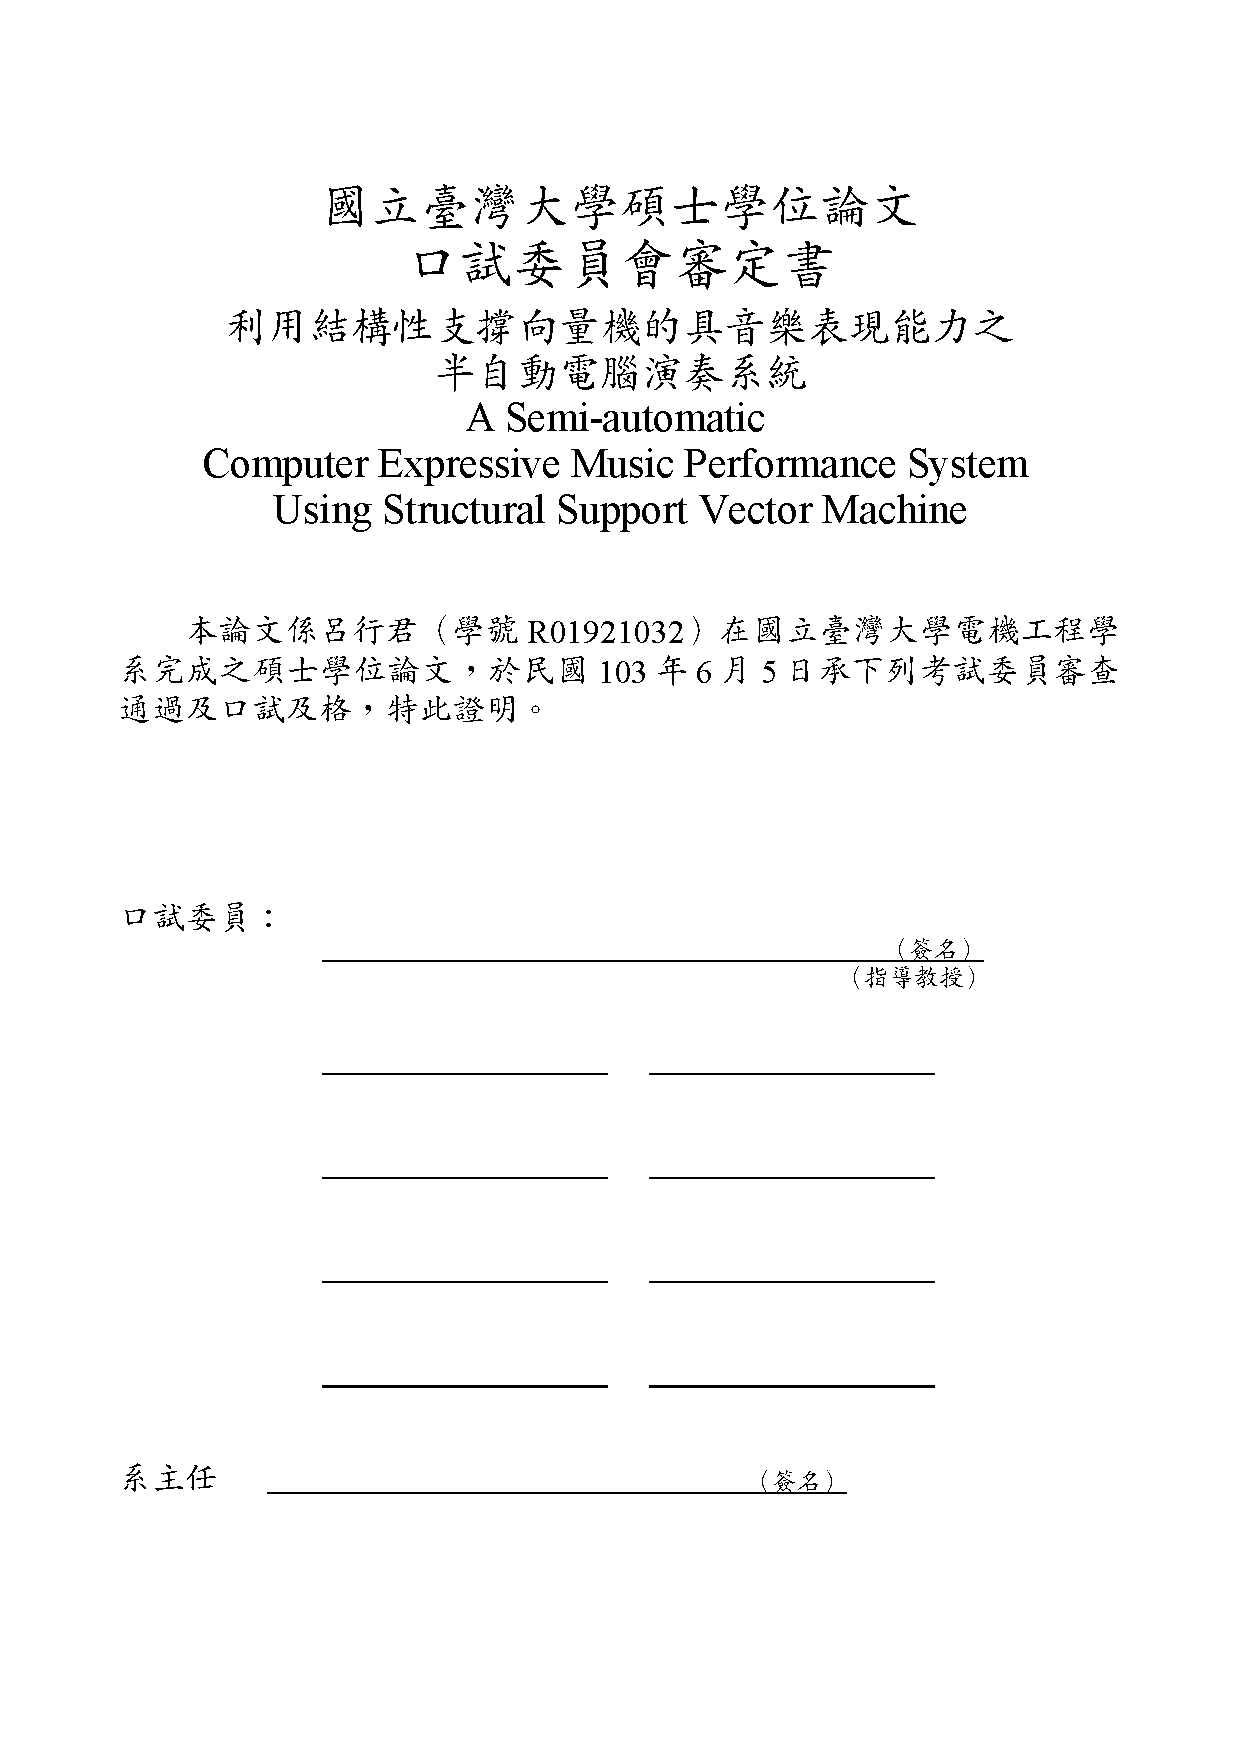
\includepdf[pages={1}]{cert.pdf}
    \end{verbatim}
    \item 浮水印:\\
    資料夾已經附上浮水印檔案了,若學校有更改,到請到台大圖書館網頁的\href{http://etds.lib.ntu.edu.tw/etdsystem/submit/submitLogin}{電子論文服務}下載\href{http://etds.lib.ntu.edu.tw/files/watermark.pdf}{pdf格式的浮水印}到此範本所在資料夾。若要開啟關閉浮水印功能,即自行刪去或加上下面位於\href{run:./thesis.tex}{thesis.tex}指令的註解符號\texttt{\%}
    \begin{verbatim}
%\CenterWallPaper{0.174}{watermark.pdf}
%\setlength{\wpXoffset}{6.1725cm}
%\setlength{\wpYoffset}{10.5225cm}
    \end{verbatim}
    \item 單面印刷與雙面印刷:\\
    此範本為單面印刷,若論文頁數超過80頁,依規定需要用雙面印刷,此時只需把thesis.tex裡的
    \begin{verbatim}
\documentclass[a4paper, 12pt, oneside]{book}
改成
\documentclass[a4paper, 12pt, twoside]{book}
    \end{verbatim}
        \item 如何加入附錄?\\
    在\href{run:./thesis.tex}{thesis.tex}裡,依需求選擇input或include,刪去\texttt{\%}符號來輸入附錄章節
    \begin{verbatim}
%----------- Input your appendix here  -----------
%\chapter{First appendix title}

Open and edit \href{run:./AppendixA.tex}{AppendixA.tex}
%or %chapter cite  == \include
%\chapter{First appendix title}

Open and edit \href{run:./AppendixA.tex}{AppendixA.tex}
    \end{verbatim}
    在章節檔\texttt{AppendixA.tex}裡,開頭打
    \begin{verbatim}
\chapter{First appendix title}
    \end{verbatim}
    即可,以此類推。    
        \item 系上規定論文圖表須全部放到最後獨立出來的章節,且章節不出現在目錄中:\\
    在\href{run:./thesis.tex}{thesis.tex}裡,依需求選擇input或include,刪去\texttt{\%}符號來輸入圖表章節
    \begin{verbatim}    
%----------- Input your Figure chapter here  -----------
%\chapter*{}  %加星號隱藏標題

%----------- 重新設定counter格式,章節圖檔和表格的計數器格式皆為1…9 -----------
\renewcommand{\thefigure}{\arabic{chapter}.\arabic{figure}} 
\renewcommand{\thetable}{\arabic{chapter}.\arabic{table}} 
%--------- Input your main figures and tables here  ---------
\setcounter{chapter}{3}%使章節couter切回3,第三章圖放在此行之後
\setcounter{figure}{1}  %使圖檔couter切回1
\setcounter{table}{1}  %使表格couter切回1

\begin{figure}[!]
\centering
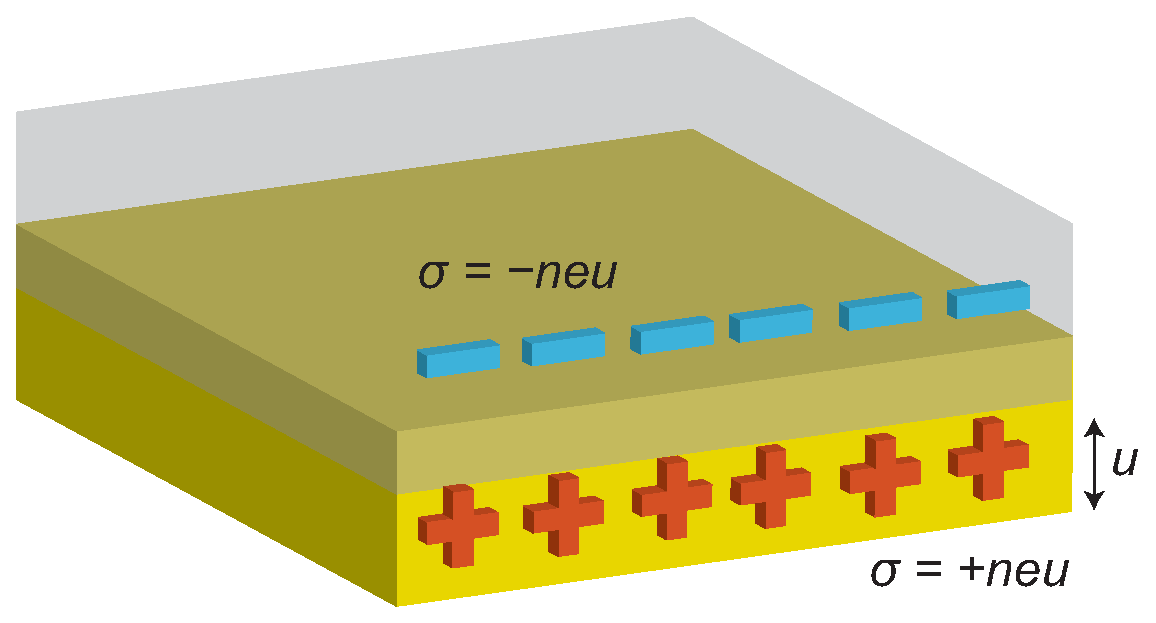
\includegraphics[scale=0.5]{THM/bulk.eps}
\caption{\label{fig:bulk}Longitudinal collective oscillations of the conduction electrons of a metal (Volume plasmons)}
\end{figure}

\begin{table}[!]\begin{center}
\caption{Table Example 1}
\begin{tabularx}{8cm}{llX}
\hline
Start & End  & Character Block Name \\
\hline
3400  & 4DB5 & CJK Unified Ideographs Extension A \\
4E00  & 9FFF & CJK Unified Ideographs \\
\hline
\end{tabularx}
 \end{center}\end{table}
 
\begin{figure}[!]
\centering
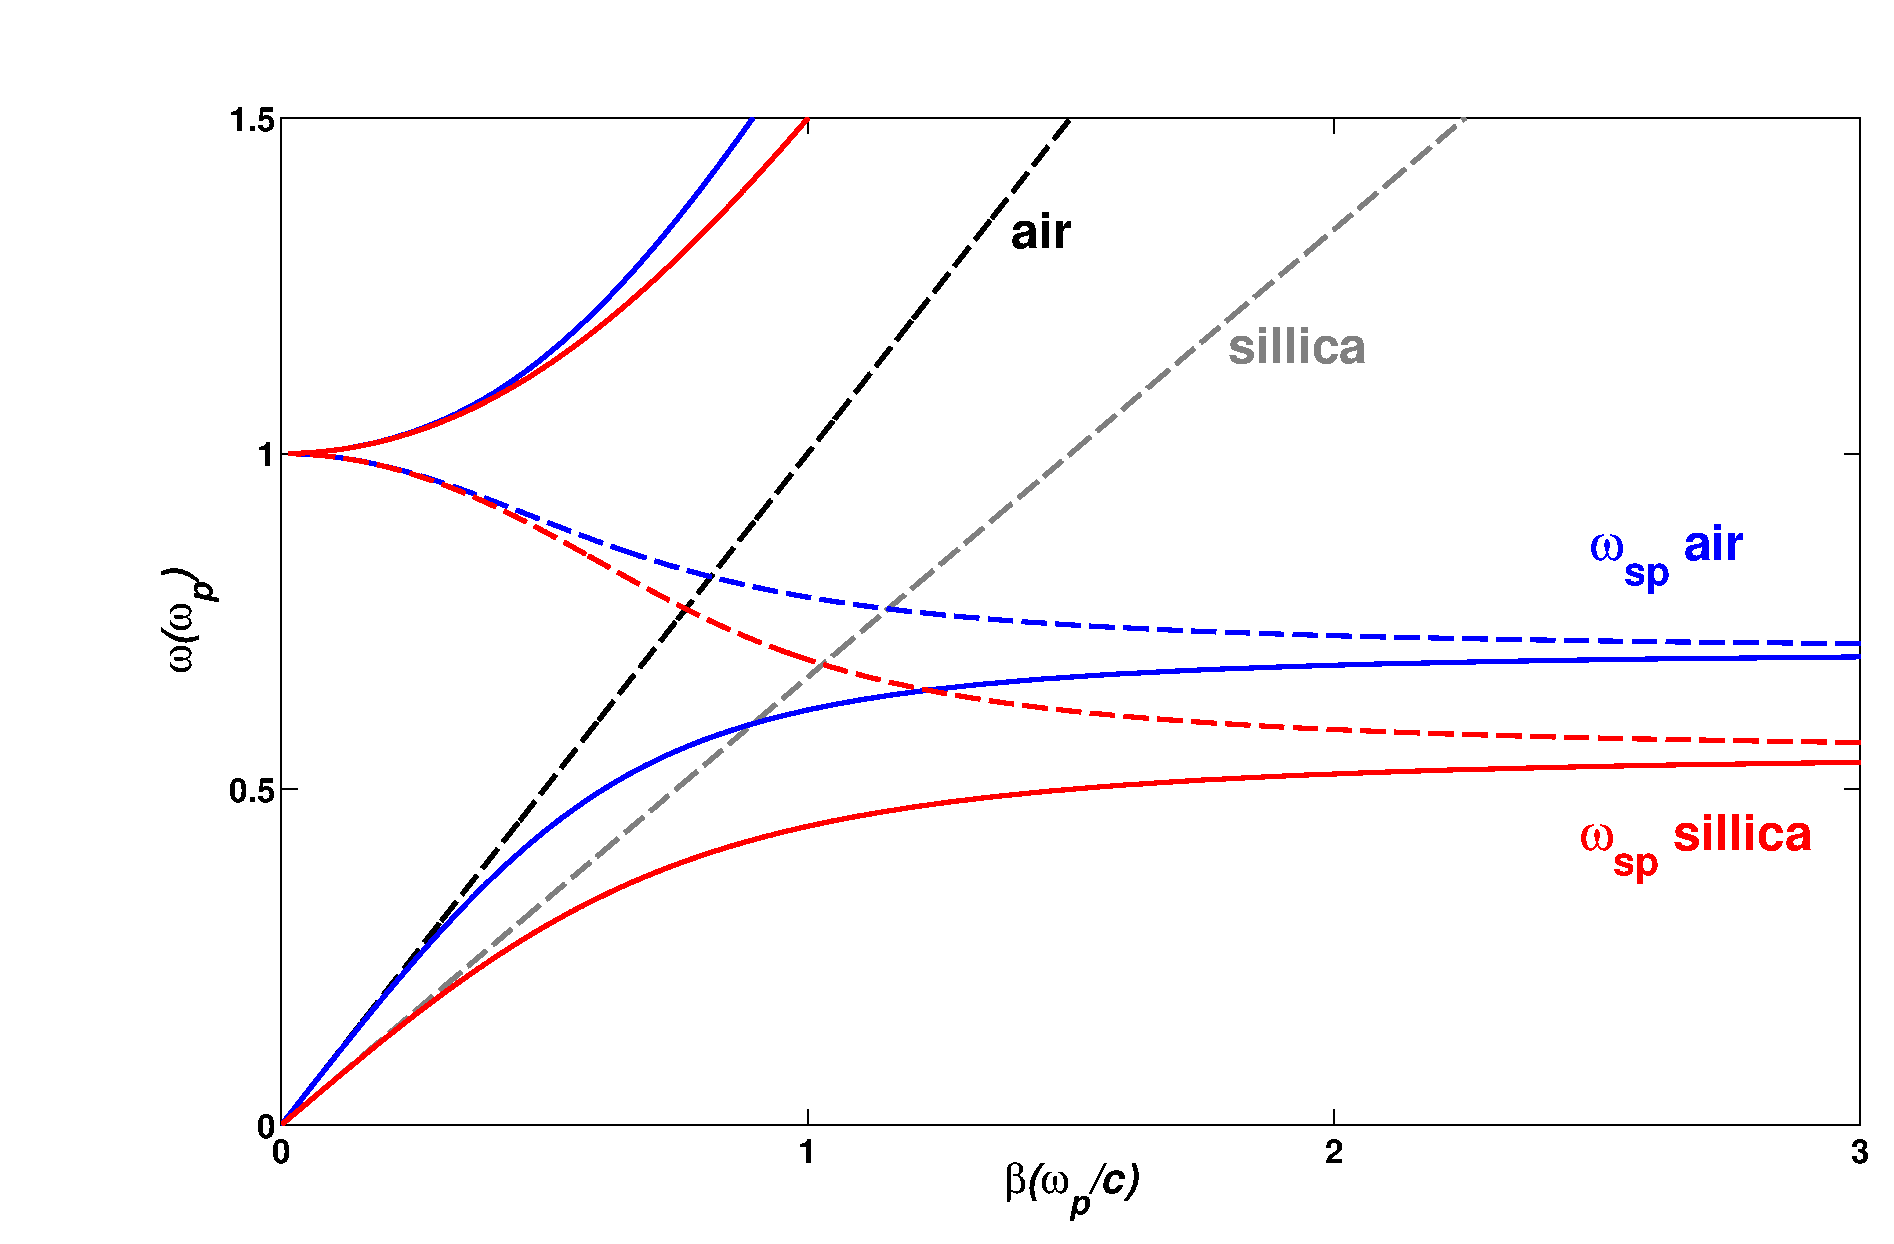
\includegraphics[scale=0.4]{THM/SPPdisp.eps}
\caption{\label{fig:SPPdisp}Dispersion relation of SPPs at the interface between a Drude metal with negligible collision frequency and air (blue curves) and silica (red curves).}
\end{figure}

\setcounter{chapter}{4}  %使章節couter切回4,第4章圖放在此行之後
\setcounter{figure}{1}  %使圖檔couter切回1

\begin{figure}[!]
\centering
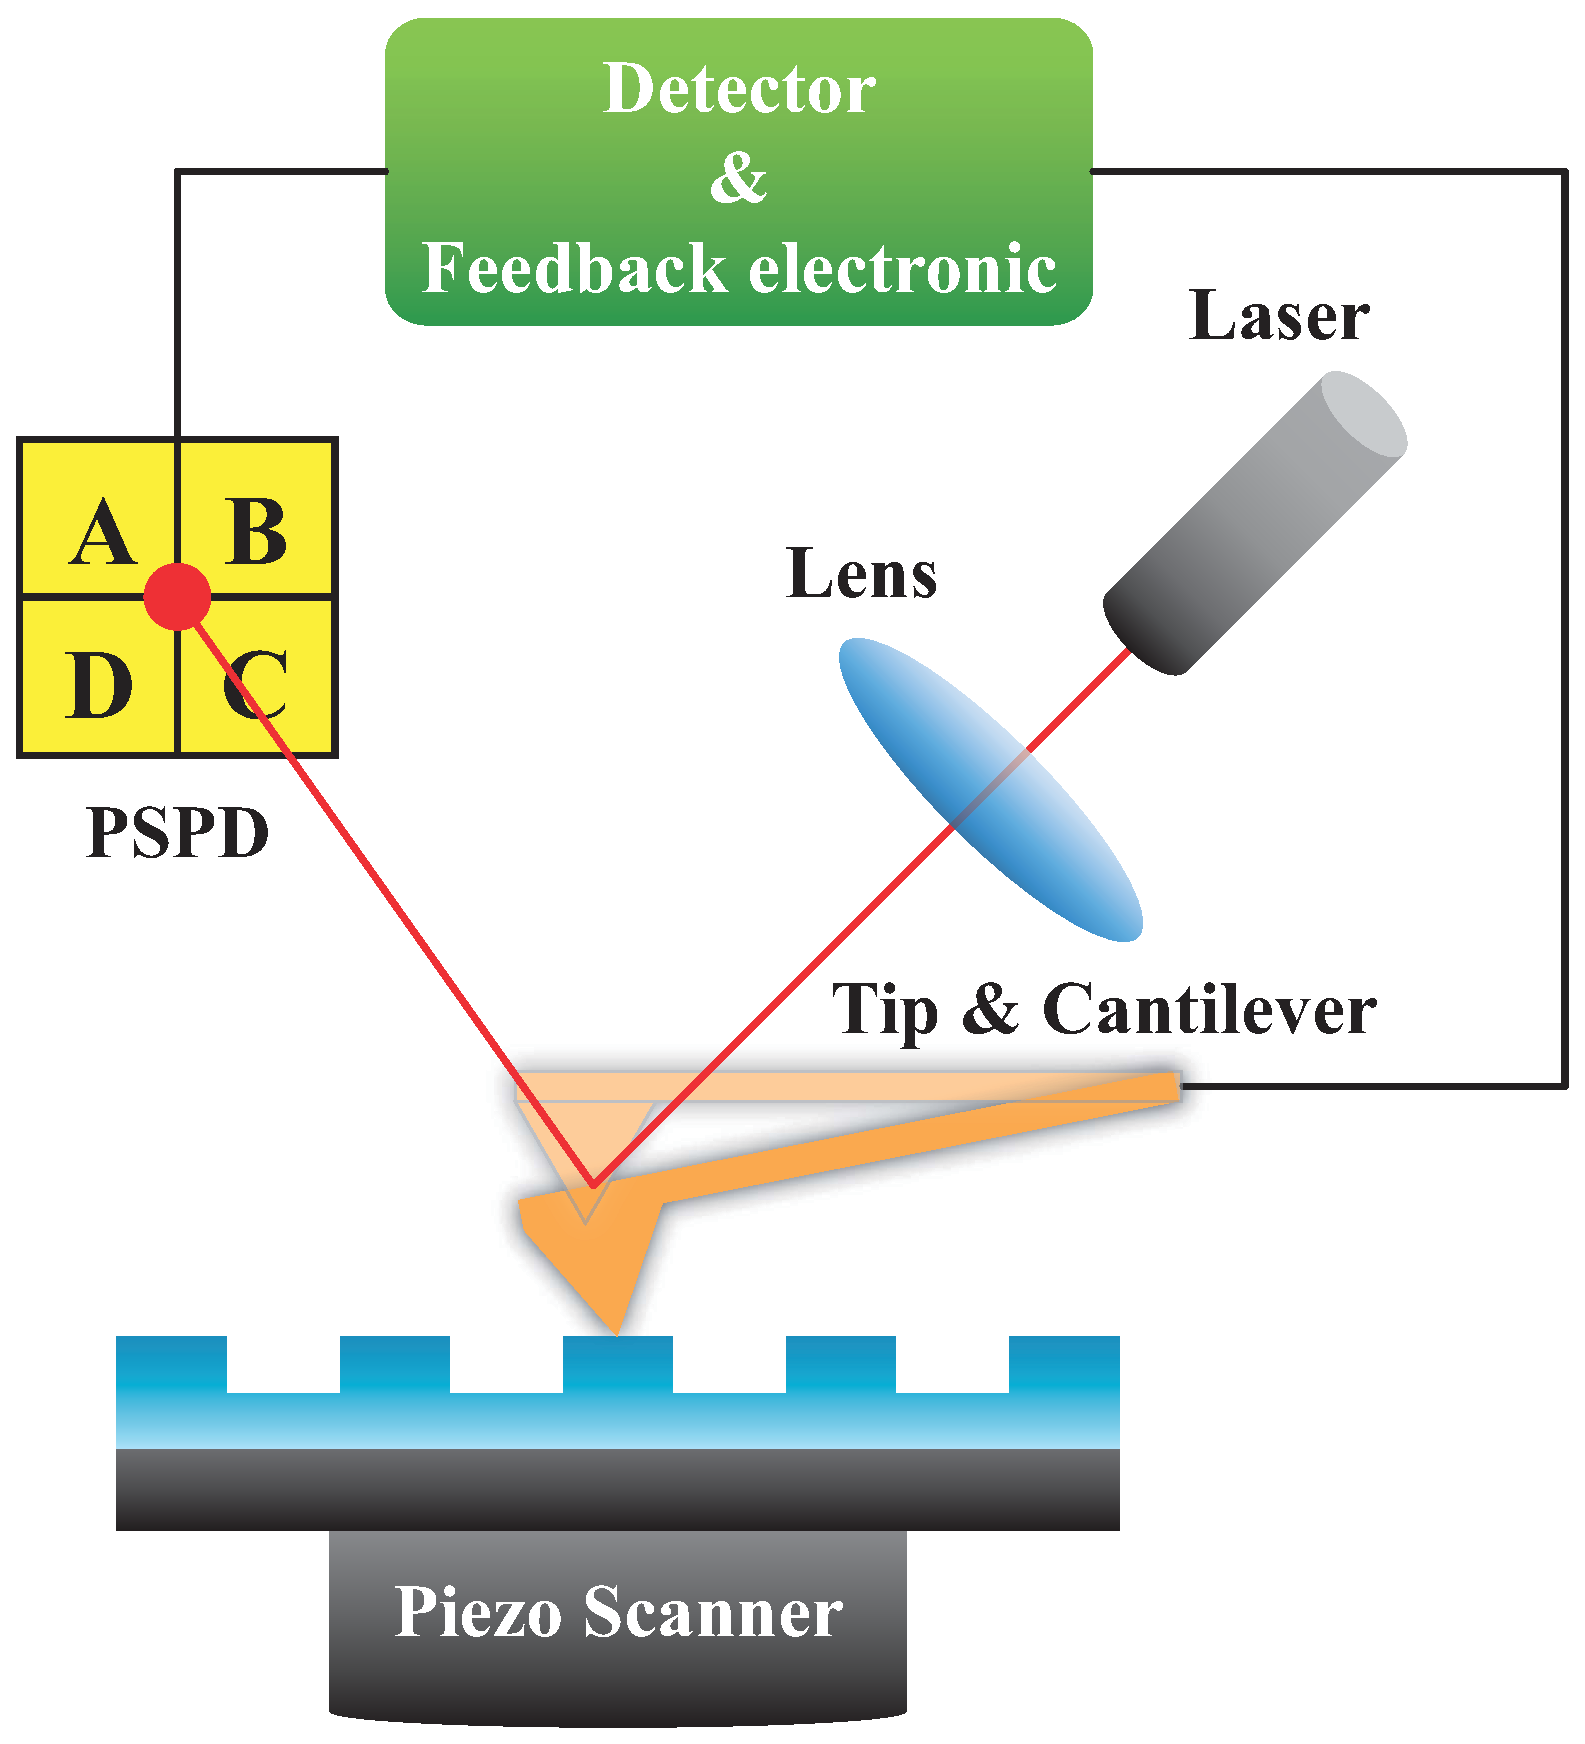
\includegraphics[scale=0.35]{EXP/afm1.eps}
\caption{\label{fig:afm1}Schematic of atomic force microscopy.}
\end{figure}

\begin{figure}[!]
\centering
\includegraphics[scale=0.6]{EXP/afm3.eps}
\caption{\label{fig:afm3}Sketch of tip-sample forces.}
\end{figure}

%----------- 重新設定counter格式,章節的計數器格式為A…Z,圖檔和表格的格式皆為1…9 -----------
\renewcommand{\thefigure}{\Alph{chapter}.\arabic{figure}} 
\renewcommand{\thetable}{\Alph{chapter}.\arabic{table}}
%--------- Input your appendix figures and tables here  ---------
\setcounter{chapter}{3}%使章節couter切回3,附錄3圖放在此行之後
\setcounter{figure}{1}  %使圖檔couter切回1
\setcounter{table}{1}  %使表格couter切回1

\begin{figure}[!]
\centering
\includegraphics[scale=0.5]{THM/bulk.eps}
\caption{\label{fig:bulk}Longitudinal collective oscillations of the conduction electrons of a metal (Volume plasmons)}
\end{figure}

\begin{table}[!]\begin{center}
\caption{Table Example 1}
\begin{tabularx}{8cm}{llX}
\hline
Start & End  & Character Block Name \\
\hline
3400  & 4DB5 & CJK Unified Ideographs Extension A \\
4E00  & 9FFF & CJK Unified Ideographs \\
\hline
\end{tabularx}
\end{center}\end{table}

\begin{figure}[!]
\centering
\includegraphics[scale=0.4]{THM/SPPdisp.eps}
\caption{\label{fig:SPPdisp}Dispersion relation of SPPs at the interface between a Drude metal with negligible collision frequency and air (blue curves) and silica (red curves).}
\end{figure}

\setcounter{chapter}{4}  %使章節couter切回4,附錄4章圖放在此行之後
\setcounter{figure}{1}  %使圖檔couter切回1

\begin{figure}[!]
\centering
\includegraphics[scale=0.35]{EXP/afm1.eps}
\caption{\label{fig:afm1}Schematic of atomic force microscopy.}
\end{figure}

\begin{figure}[!]
\centering
\includegraphics[scale=0.6]{EXP/afm3.eps}
\caption{\label{fig:afm3}Sketch of tip-sample forces.}
\end{figure} 
%chapter cite  == \include
%\chapter*{}  %加星號隱藏標題

%----------- 重新設定counter格式,章節圖檔和表格的計數器格式皆為1…9 -----------
\renewcommand{\thefigure}{\arabic{chapter}.\arabic{figure}} 
\renewcommand{\thetable}{\arabic{chapter}.\arabic{table}} 
%--------- Input your main figures and tables here  ---------
\setcounter{chapter}{3}%使章節couter切回3,第三章圖放在此行之後
\setcounter{figure}{1}  %使圖檔couter切回1
\setcounter{table}{1}  %使表格couter切回1

\begin{figure}[!]
\centering
\includegraphics[scale=0.5]{THM/bulk.eps}
\caption{\label{fig:bulk}Longitudinal collective oscillations of the conduction electrons of a metal (Volume plasmons)}
\end{figure}

\begin{table}[!]\begin{center}
\caption{Table Example 1}
\begin{tabularx}{8cm}{llX}
\hline
Start & End  & Character Block Name \\
\hline
3400  & 4DB5 & CJK Unified Ideographs Extension A \\
4E00  & 9FFF & CJK Unified Ideographs \\
\hline
\end{tabularx}
 \end{center}\end{table}
 
\begin{figure}[!]
\centering
\includegraphics[scale=0.4]{THM/SPPdisp.eps}
\caption{\label{fig:SPPdisp}Dispersion relation of SPPs at the interface between a Drude metal with negligible collision frequency and air (blue curves) and silica (red curves).}
\end{figure}

\setcounter{chapter}{4}  %使章節couter切回4,第4章圖放在此行之後
\setcounter{figure}{1}  %使圖檔couter切回1

\begin{figure}[!]
\centering
\includegraphics[scale=0.35]{EXP/afm1.eps}
\caption{\label{fig:afm1}Schematic of atomic force microscopy.}
\end{figure}

\begin{figure}[!]
\centering
\includegraphics[scale=0.6]{EXP/afm3.eps}
\caption{\label{fig:afm3}Sketch of tip-sample forces.}
\end{figure}

%----------- 重新設定counter格式,章節的計數器格式為A…Z,圖檔和表格的格式皆為1…9 -----------
\renewcommand{\thefigure}{\Alph{chapter}.\arabic{figure}} 
\renewcommand{\thetable}{\Alph{chapter}.\arabic{table}}
%--------- Input your appendix figures and tables here  ---------
\setcounter{chapter}{3}%使章節couter切回3,附錄3圖放在此行之後
\setcounter{figure}{1}  %使圖檔couter切回1
\setcounter{table}{1}  %使表格couter切回1

\begin{figure}[!]
\centering
\includegraphics[scale=0.5]{THM/bulk.eps}
\caption{\label{fig:bulk}Longitudinal collective oscillations of the conduction electrons of a metal (Volume plasmons)}
\end{figure}

\begin{table}[!]\begin{center}
\caption{Table Example 1}
\begin{tabularx}{8cm}{llX}
\hline
Start & End  & Character Block Name \\
\hline
3400  & 4DB5 & CJK Unified Ideographs Extension A \\
4E00  & 9FFF & CJK Unified Ideographs \\
\hline
\end{tabularx}
\end{center}\end{table}

\begin{figure}[!]
\centering
\includegraphics[scale=0.4]{THM/SPPdisp.eps}
\caption{\label{fig:SPPdisp}Dispersion relation of SPPs at the interface between a Drude metal with negligible collision frequency and air (blue curves) and silica (red curves).}
\end{figure}

\setcounter{chapter}{4}  %使章節couter切回4,附錄4章圖放在此行之後
\setcounter{figure}{1}  %使圖檔couter切回1

\begin{figure}[!]
\centering
\includegraphics[scale=0.35]{EXP/afm1.eps}
\caption{\label{fig:afm1}Schematic of atomic force microscopy.}
\end{figure}

\begin{figure}[!]
\centering
\includegraphics[scale=0.6]{EXP/afm3.eps}
\caption{\label{fig:afm3}Sketch of tip-sample forces.}
\end{figure}
    \end{verbatim}
    在章節檔\href{run:./EndFigTab.tex}{EndFigTab.tex}裡有範例和說明可供參考,要注意正文的圖表和附錄的圖表要分清楚,即在\href{run:./EndFigTab.tex}{EndFigTab.tex}內
    \begin{verbatim}    
\renewcommand{\thefigure}{\arabic{chapter}.\arabic{figure}} 
\renewcommand{\thetable}{\arabic{chapter}.\arabic{table}} 
%--- Input your main figures and tables here  ---
    \end{verbatim}
    這幾行之後章節計數器格式已切換為1\dots 9,放正文的圖表 ,
     \begin{verbatim}    
\renewcommand{\thefigure}{\Alph{chapter}.\arabic{figure}} 
\renewcommand{\thetable}{\Alph{chapter}.\arabic{table}}
%--- Input your appendix figures and tables here  ---
    \end{verbatim}
    這幾行之後章節計數器格式已切換為A\dots Z,放附錄的圖表。另外要取消圖表的浮動功能,才能讓圖表按照指令出現順序排好,即把平常使用的圖表指令
    \begin{verbatim}    
\begin{figure}[htb]
...
\begin{table}[htb]
    \end{verbatim}
    改成
     \begin{verbatim}    
\begin{figure}[!]
...
\begin{table}[!]
    \end{verbatim}
    剩下的只要注意章節圖表的計數器設定即可。\texttt{\textbackslash ref}和\texttt{\textbackslash label}指令可以在此圖表章節與正文章節使用。
     \item 如果我想要修改margin(文字邊界)的話,可以從哪裡下手呢?\\
     請打開\href{run:./ntu.sty}{ntu.sty}修改下面這行的上下左右參數即可:
    \begin{verbatim}
\RequirePackage[top=3cm,left=3cm,bottom=2cm,right=3cm]{geometry}
    \end{verbatim}
    \item 我想引用Twomey (1974): Pollution and planetary albedo這篇論文,如何用\texttt{\textbackslash cite}引用它的時候在內文顯示Twomey (1974) [編號] ?\\
    建議使用natbib套件,參考資料如下:\\
    \href{http://en.wikibooks.org/wiki/LaTeX/Bibliography_Management}{LaTeX/Bibliography Management}\\
    \href{http://nodonn.tipido.net/bibstyle.php}{Overview of Bibtex-Styles}\\
    \href{http://merkel.zoneo.net/Latex/natbib.php}{Reference sheet for natbib usage }\\
 \item \XeTeX\ :\\
    此範本中文字體使用\XeTeX\ 轉換,細節請參考\href{http://www.hitripod.com/blog/}{Hitripod}寫的\href{http://www.hitripod.com/blog/2011/04/xetex-chinese-font-cjk-latex/}{ 
XeTeX:解決 LaTeX 惱人的中文字型問題}。
    \end{enumerate} 
    \end{enumerate} 

%----------- Have a fractal fern? -----------
%\begin{pspicture}
%\psFern[scale=30,maxIter=100000,linecolor=Green]
%\end{pspicture}


\end{appendices}

\backmatter



%----------- Input your Fig. chapter here  -----------
%\chapter*{}  %加星號隱藏標題

%----------- 重新設定counter格式,章節圖檔和表格的計數器格式皆為1…9 -----------
\renewcommand{\thefigure}{\arabic{chapter}.\arabic{figure}} 
\renewcommand{\thetable}{\arabic{chapter}.\arabic{table}} 
%--------- Input your main figures and tables here  ---------
\setcounter{chapter}{3}%使章節couter切回3,第三章圖放在此行之後
\setcounter{figure}{1}  %使圖檔couter切回1
\setcounter{table}{1}  %使表格couter切回1

\begin{figure}[!]
\centering
\includegraphics[scale=0.5]{THM/bulk.eps}
\caption{\label{fig:bulk}Longitudinal collective oscillations of the conduction electrons of a metal (Volume plasmons)}
\end{figure}

\begin{table}[!]\begin{center}
\caption{Table Example 1}
\begin{tabularx}{8cm}{llX}
\hline
Start & End  & Character Block Name \\
\hline
3400  & 4DB5 & CJK Unified Ideographs Extension A \\
4E00  & 9FFF & CJK Unified Ideographs \\
\hline
\end{tabularx}
 \end{center}\end{table}
 
\begin{figure}[!]
\centering
\includegraphics[scale=0.4]{THM/SPPdisp.eps}
\caption{\label{fig:SPPdisp}Dispersion relation of SPPs at the interface between a Drude metal with negligible collision frequency and air (blue curves) and silica (red curves).}
\end{figure}

\setcounter{chapter}{4}  %使章節couter切回4,第4章圖放在此行之後
\setcounter{figure}{1}  %使圖檔couter切回1

\begin{figure}[!]
\centering
\includegraphics[scale=0.35]{EXP/afm1.eps}
\caption{\label{fig:afm1}Schematic of atomic force microscopy.}
\end{figure}

\begin{figure}[!]
\centering
\includegraphics[scale=0.6]{EXP/afm3.eps}
\caption{\label{fig:afm3}Sketch of tip-sample forces.}
\end{figure}

%----------- 重新設定counter格式,章節的計數器格式為A…Z,圖檔和表格的格式皆為1…9 -----------
\renewcommand{\thefigure}{\Alph{chapter}.\arabic{figure}} 
\renewcommand{\thetable}{\Alph{chapter}.\arabic{table}}
%--------- Input your appendix figures and tables here  ---------
\setcounter{chapter}{3}%使章節couter切回3,附錄3圖放在此行之後
\setcounter{figure}{1}  %使圖檔couter切回1
\setcounter{table}{1}  %使表格couter切回1

\begin{figure}[!]
\centering
\includegraphics[scale=0.5]{THM/bulk.eps}
\caption{\label{fig:bulk}Longitudinal collective oscillations of the conduction electrons of a metal (Volume plasmons)}
\end{figure}

\begin{table}[!]\begin{center}
\caption{Table Example 1}
\begin{tabularx}{8cm}{llX}
\hline
Start & End  & Character Block Name \\
\hline
3400  & 4DB5 & CJK Unified Ideographs Extension A \\
4E00  & 9FFF & CJK Unified Ideographs \\
\hline
\end{tabularx}
\end{center}\end{table}

\begin{figure}[!]
\centering
\includegraphics[scale=0.4]{THM/SPPdisp.eps}
\caption{\label{fig:SPPdisp}Dispersion relation of SPPs at the interface between a Drude metal with negligible collision frequency and air (blue curves) and silica (red curves).}
\end{figure}

\setcounter{chapter}{4}  %使章節couter切回4,附錄4章圖放在此行之後
\setcounter{figure}{1}  %使圖檔couter切回1

\begin{figure}[!]
\centering
\includegraphics[scale=0.35]{EXP/afm1.eps}
\caption{\label{fig:afm1}Schematic of atomic force microscopy.}
\end{figure}

\begin{figure}[!]
\centering
\includegraphics[scale=0.6]{EXP/afm3.eps}
\caption{\label{fig:afm3}Sketch of tip-sample forces.}
\end{figure} 
%chapter cite  == \include
%\chapter*{}  %加星號隱藏標題

%----------- 重新設定counter格式,章節圖檔和表格的計數器格式皆為1…9 -----------
\renewcommand{\thefigure}{\arabic{chapter}.\arabic{figure}} 
\renewcommand{\thetable}{\arabic{chapter}.\arabic{table}} 
%--------- Input your main figures and tables here  ---------
\setcounter{chapter}{3}%使章節couter切回3,第三章圖放在此行之後
\setcounter{figure}{1}  %使圖檔couter切回1
\setcounter{table}{1}  %使表格couter切回1

\begin{figure}[!]
\centering
\includegraphics[scale=0.5]{THM/bulk.eps}
\caption{\label{fig:bulk}Longitudinal collective oscillations of the conduction electrons of a metal (Volume plasmons)}
\end{figure}

\begin{table}[!]\begin{center}
\caption{Table Example 1}
\begin{tabularx}{8cm}{llX}
\hline
Start & End  & Character Block Name \\
\hline
3400  & 4DB5 & CJK Unified Ideographs Extension A \\
4E00  & 9FFF & CJK Unified Ideographs \\
\hline
\end{tabularx}
 \end{center}\end{table}
 
\begin{figure}[!]
\centering
\includegraphics[scale=0.4]{THM/SPPdisp.eps}
\caption{\label{fig:SPPdisp}Dispersion relation of SPPs at the interface between a Drude metal with negligible collision frequency and air (blue curves) and silica (red curves).}
\end{figure}

\setcounter{chapter}{4}  %使章節couter切回4,第4章圖放在此行之後
\setcounter{figure}{1}  %使圖檔couter切回1

\begin{figure}[!]
\centering
\includegraphics[scale=0.35]{EXP/afm1.eps}
\caption{\label{fig:afm1}Schematic of atomic force microscopy.}
\end{figure}

\begin{figure}[!]
\centering
\includegraphics[scale=0.6]{EXP/afm3.eps}
\caption{\label{fig:afm3}Sketch of tip-sample forces.}
\end{figure}

%----------- 重新設定counter格式,章節的計數器格式為A…Z,圖檔和表格的格式皆為1…9 -----------
\renewcommand{\thefigure}{\Alph{chapter}.\arabic{figure}} 
\renewcommand{\thetable}{\Alph{chapter}.\arabic{table}}
%--------- Input your appendix figures and tables here  ---------
\setcounter{chapter}{3}%使章節couter切回3,附錄3圖放在此行之後
\setcounter{figure}{1}  %使圖檔couter切回1
\setcounter{table}{1}  %使表格couter切回1

\begin{figure}[!]
\centering
\includegraphics[scale=0.5]{THM/bulk.eps}
\caption{\label{fig:bulk}Longitudinal collective oscillations of the conduction electrons of a metal (Volume plasmons)}
\end{figure}

\begin{table}[!]\begin{center}
\caption{Table Example 1}
\begin{tabularx}{8cm}{llX}
\hline
Start & End  & Character Block Name \\
\hline
3400  & 4DB5 & CJK Unified Ideographs Extension A \\
4E00  & 9FFF & CJK Unified Ideographs \\
\hline
\end{tabularx}
\end{center}\end{table}

\begin{figure}[!]
\centering
\includegraphics[scale=0.4]{THM/SPPdisp.eps}
\caption{\label{fig:SPPdisp}Dispersion relation of SPPs at the interface between a Drude metal with negligible collision frequency and air (blue curves) and silica (red curves).}
\end{figure}

\setcounter{chapter}{4}  %使章節couter切回4,附錄4章圖放在此行之後
\setcounter{figure}{1}  %使圖檔couter切回1

\begin{figure}[!]
\centering
\includegraphics[scale=0.35]{EXP/afm1.eps}
\caption{\label{fig:afm1}Schematic of atomic force microscopy.}
\end{figure}

\begin{figure}[!]
\centering
\includegraphics[scale=0.6]{EXP/afm3.eps}
\caption{\label{fig:afm3}Sketch of tip-sample forces.}
\end{figure}

\end{document}
